\documentclass[a4paper]{book}
\usepackage{a4wide}
\usepackage{makeidx}
\usepackage{graphicx}
\usepackage{multicol}
\usepackage{float}
\usepackage{listings}
\usepackage{color}
\usepackage{textcomp}
\usepackage{alltt}
\usepackage{times}
\usepackage{ifpdf}
\ifpdf
\usepackage[pdftex,
            pagebackref=true,
            colorlinks=true,
            linkcolor=blue,
            unicode
           ]{hyperref}
\else
\usepackage[ps2pdf,
            pagebackref=true,
            colorlinks=true,
            linkcolor=blue,
            unicode
           ]{hyperref}
\usepackage{pspicture}
\fi
\usepackage[utf8]{inputenc}
\usepackage{doxygen}
\lstset{language=C++,inputencoding=utf8,basicstyle=\footnotesize,breaklines=true,breakatwhitespace=true,tabsize=8,numbers=left }
\makeindex
\setcounter{tocdepth}{3}
\renewcommand{\footrulewidth}{0.4pt}
\begin{document}
\hypersetup{pageanchor=false}
\begin{titlepage}
\vspace*{7cm}
\begin{center}
{\Large wGui }\\
\vspace*{1cm}
{\large Generated by Doxygen 1.7.1}\\
\vspace*{0.5cm}
{\small Thu Feb 17 2011 09:18:18}\\
\end{center}
\end{titlepage}
\clearemptydoublepage
\pagenumbering{roman}
\tableofcontents
\clearemptydoublepage
\pagenumbering{arabic}
\hypersetup{pageanchor=true}
\chapter{Class Index}
\section{Class Hierarchy}
This inheritance list is sorted roughly, but not completely, alphabetically:\begin{DoxyCompactList}
\item \contentsline{section}{clsContext}{\pageref{classclsContext}}{}
\item \contentsline{section}{clsEventHandlers}{\pageref{classclsEventHandlers}}{}
\item \contentsline{section}{clsFunctions}{\pageref{classclsFunctions}}{}
\item \contentsline{section}{clsPage}{\pageref{classclsPage}}{}
\item \contentsline{section}{clsRequests}{\pageref{classclsRequests}}{}
\item \contentsline{section}{clsValidator}{\pageref{classclsValidator}}{}
\item \contentsline{section}{myExternalClass}{\pageref{classmyExternalClass}}{}
\item \contentsline{section}{myObjectTest}{\pageref{classmyObjectTest}}{}
\item \contentsline{section}{myPreObject}{\pageref{classmyPreObject}}{}
\item \contentsline{section}{objectMethodsTest}{\pageref{classobjectMethodsTest}}{}
\begin{DoxyCompactList}
\item \contentsline{section}{objectMethodsTest2}{\pageref{classobjectMethodsTest2}}{}
\end{DoxyCompactList}
\item \contentsline{section}{xajax}{\pageref{classxajax}}{}
\begin{DoxyCompactList}
\item \contentsline{section}{legacyXajax}{\pageref{classlegacyXajax}}{}
\end{DoxyCompactList}
\item \contentsline{section}{xajaxArgumentManager}{\pageref{classxajaxArgumentManager}}{}
\item \contentsline{section}{xajaxCall}{\pageref{classxajaxCall}}{}
\item \contentsline{section}{xajaxCallableObject}{\pageref{classxajaxCallableObject}}{}
\item \contentsline{section}{xajaxControl}{\pageref{classxajaxControl}}{}
\begin{DoxyCompactList}
\item \contentsline{section}{clsArea}{\pageref{classclsArea}}{}
\item \contentsline{section}{clsBase}{\pageref{classclsBase}}{}
\item \contentsline{section}{clsBr}{\pageref{classclsBr}}{}
\item \contentsline{section}{clsCol}{\pageref{classclsCol}}{}
\item \contentsline{section}{clsFrame}{\pageref{classclsFrame}}{}
\item \contentsline{section}{clsHr}{\pageref{classclsHr}}{}
\item \contentsline{section}{clsImg}{\pageref{classclsImg}}{}
\item \contentsline{section}{clsInput}{\pageref{classclsInput}}{}
\begin{DoxyCompactList}
\item \contentsline{section}{clsInputWithLabel}{\pageref{classclsInputWithLabel}}{}
\end{DoxyCompactList}
\item \contentsline{section}{clsLink}{\pageref{classclsLink}}{}
\item \contentsline{section}{clsLiteral}{\pageref{classclsLiteral}}{}
\item \contentsline{section}{clsMeta}{\pageref{classclsMeta}}{}
\item \contentsline{section}{clsMutuallyExclusiveButton}{\pageref{classclsMutuallyExclusiveButton}}{}
\item \contentsline{section}{clsParam}{\pageref{classclsParam}}{}
\item \contentsline{section}{xajaxControlContainer}{\pageref{classxajaxControlContainer}}{}
\begin{DoxyCompactList}
\item \contentsline{section}{clsAnchor}{\pageref{classclsAnchor}}{}
\item \contentsline{section}{clsBody}{\pageref{classclsBody}}{}
\item \contentsline{section}{clsButton}{\pageref{classclsButton}}{}
\item \contentsline{section}{clsCaption}{\pageref{classclsCaption}}{}
\item \contentsline{section}{clsColgroup}{\pageref{classclsColgroup}}{}
\item \contentsline{section}{clsDd}{\pageref{classclsDd}}{}
\item \contentsline{section}{clsDiv}{\pageref{classclsDiv}}{}
\item \contentsline{section}{clsDl}{\pageref{classclsDl}}{}
\item \contentsline{section}{clsDoctype}{\pageref{classclsDoctype}}{}
\item \contentsline{section}{clsDocument}{\pageref{classclsDocument}}{}
\item \contentsline{section}{clsDt}{\pageref{classclsDt}}{}
\item \contentsline{section}{clsFieldset}{\pageref{classclsFieldset}}{}
\item \contentsline{section}{clsForm}{\pageref{classclsForm}}{}
\item \contentsline{section}{clsFrameset}{\pageref{classclsFrameset}}{}
\item \contentsline{section}{clsHead}{\pageref{classclsHead}}{}
\item \contentsline{section}{clsHeadline}{\pageref{classclsHeadline}}{}
\item \contentsline{section}{clsHtml}{\pageref{classclsHtml}}{}
\item \contentsline{section}{clsIframe}{\pageref{classclsIframe}}{}
\item \contentsline{section}{clsInlineContainer}{\pageref{classclsInlineContainer}}{}
\begin{DoxyCompactList}
\item \contentsline{section}{clsAbbr}{\pageref{classclsAbbr}}{}
\item \contentsline{section}{clsAcronym}{\pageref{classclsAcronym}}{}
\item \contentsline{section}{clsAddress}{\pageref{classclsAddress}}{}
\item \contentsline{section}{clsBig}{\pageref{classclsBig}}{}
\item \contentsline{section}{clsBlockquote}{\pageref{classclsBlockquote}}{}
\item \contentsline{section}{clsBold}{\pageref{classclsBold}}{}
\item \contentsline{section}{clsCite}{\pageref{classclsCite}}{}
\item \contentsline{section}{clsCode}{\pageref{classclsCode}}{}
\item \contentsline{section}{clsDel}{\pageref{classclsDel}}{}
\item \contentsline{section}{clsDfn}{\pageref{classclsDfn}}{}
\item \contentsline{section}{clsEm}{\pageref{classclsEm}}{}
\item \contentsline{section}{clsIns}{\pageref{classclsIns}}{}
\item \contentsline{section}{clsItalic}{\pageref{classclsItalic}}{}
\item \contentsline{section}{clsKbd}{\pageref{classclsKbd}}{}
\item \contentsline{section}{clsParagraph}{\pageref{classclsParagraph}}{}
\item \contentsline{section}{clsPre}{\pageref{classclsPre}}{}
\item \contentsline{section}{clsSamp}{\pageref{classclsSamp}}{}
\item \contentsline{section}{clsSmall}{\pageref{classclsSmall}}{}
\item \contentsline{section}{clsStrong}{\pageref{classclsStrong}}{}
\item \contentsline{section}{clsSub}{\pageref{classclsSub}}{}
\item \contentsline{section}{clsTt}{\pageref{classclsTt}}{}
\item \contentsline{section}{clsVar}{\pageref{classclsVar}}{}
\end{DoxyCompactList}
\item \contentsline{section}{clsLabel}{\pageref{classclsLabel}}{}
\item \contentsline{section}{clsLegend}{\pageref{classclsLegend}}{}
\item \contentsline{section}{clsLI}{\pageref{classclsLI}}{}
\item \contentsline{section}{clsList}{\pageref{classclsList}}{}
\begin{DoxyCompactList}
\item \contentsline{section}{clsOL}{\pageref{classclsOL}}{}
\item \contentsline{section}{clsUL}{\pageref{classclsUL}}{}
\end{DoxyCompactList}
\item \contentsline{section}{clsMap}{\pageref{classclsMap}}{}
\item \contentsline{section}{clsNoframes}{\pageref{classclsNoframes}}{}
\item \contentsline{section}{clsNoscript}{\pageref{classclsNoscript}}{}
\item \contentsline{section}{clsObject}{\pageref{classclsObject}}{}
\item \contentsline{section}{clsOption}{\pageref{classclsOption}}{}
\item \contentsline{section}{clsOptionGroup}{\pageref{classclsOptionGroup}}{}
\item \contentsline{section}{clsScript}{\pageref{classclsScript}}{}
\item \contentsline{section}{clsSelect}{\pageref{classclsSelect}}{}
\item \contentsline{section}{clsSpan}{\pageref{classclsSpan}}{}
\item \contentsline{section}{clsStyle}{\pageref{classclsStyle}}{}
\item \contentsline{section}{clsSup}{\pageref{classclsSup}}{}
\item \contentsline{section}{clsTable}{\pageref{classclsTable}}{}
\item \contentsline{section}{clsTableRowContainer}{\pageref{classclsTableRowContainer}}{}
\begin{DoxyCompactList}
\item \contentsline{section}{clsTbody}{\pageref{classclsTbody}}{}
\item \contentsline{section}{clsTfoot}{\pageref{classclsTfoot}}{}
\item \contentsline{section}{clsThead}{\pageref{classclsThead}}{}
\end{DoxyCompactList}
\item \contentsline{section}{clsTd}{\pageref{classclsTd}}{}
\item \contentsline{section}{clsTextArea}{\pageref{classclsTextArea}}{}
\item \contentsline{section}{clsTh}{\pageref{classclsTh}}{}
\item \contentsline{section}{clsTitle}{\pageref{classclsTitle}}{}
\item \contentsline{section}{clsTr}{\pageref{classclsTr}}{}
\end{DoxyCompactList}
\end{DoxyCompactList}
\item \contentsline{section}{xajaxCustomResponse}{\pageref{classxajaxCustomResponse}}{}
\item \contentsline{section}{xajaxEvent}{\pageref{classxajaxEvent}}{}
\item \contentsline{section}{xajaxLanguageManager}{\pageref{classxajaxLanguageManager}}{}
\item \contentsline{section}{xajaxPlugin}{\pageref{classxajaxPlugin}}{}
\begin{DoxyCompactList}
\item \contentsline{section}{xajaxRequestPlugin}{\pageref{classxajaxRequestPlugin}}{}
\begin{DoxyCompactList}
\item \contentsline{section}{xajaxCallableObjectPlugin}{\pageref{classxajaxCallableObjectPlugin}}{}
\item \contentsline{section}{xajaxEventPlugin}{\pageref{classxajaxEventPlugin}}{}
\item \contentsline{section}{xajaxFunctionPlugin}{\pageref{classxajaxFunctionPlugin}}{}
\item \contentsline{section}{xajaxIncludeClientScriptPlugin}{\pageref{classxajaxIncludeClientScriptPlugin}}{}
\item \contentsline{section}{xajaxScriptPlugin}{\pageref{classxajaxScriptPlugin}}{}
\end{DoxyCompactList}
\item \contentsline{section}{xajaxResponsePlugin}{\pageref{classxajaxResponsePlugin}}{}
\begin{DoxyCompactList}
\item \contentsline{section}{clsGoogleMap}{\pageref{classclsGoogleMap}}{}
\item \contentsline{section}{clsTableUpdater}{\pageref{classclsTableUpdater}}{}
\item \contentsline{section}{testPlugin}{\pageref{classtestPlugin}}{}
\item \contentsline{section}{testPlugin}{\pageref{classtestPlugin}}{}
\item \contentsline{section}{testScriptPlugin}{\pageref{classtestScriptPlugin}}{}
\end{DoxyCompactList}
\end{DoxyCompactList}
\item \contentsline{section}{xajaxPluginManager}{\pageref{classxajaxPluginManager}}{}
\item \contentsline{section}{xajaxRequest}{\pageref{classxajaxRequest}}{}
\begin{DoxyCompactList}
\item \contentsline{section}{xajaxCustomRequest}{\pageref{classxajaxCustomRequest}}{}
\end{DoxyCompactList}
\item \contentsline{section}{xajaxResponse}{\pageref{classxajaxResponse}}{}
\begin{DoxyCompactList}
\item \contentsline{section}{customXajaxResponse}{\pageref{classcustomXajaxResponse}}{}
\item \contentsline{section}{legacyXajaxResponse}{\pageref{classlegacyXajaxResponse}}{}
\end{DoxyCompactList}
\item \contentsline{section}{xajaxResponseManager}{\pageref{classxajaxResponseManager}}{}
\item \contentsline{section}{xajaxUserFunction}{\pageref{classxajaxUserFunction}}{}
\end{DoxyCompactList}

\chapter{Class Index}
\section{Class List}
Here are the classes, structs, unions and interfaces with brief descriptions:\begin{DoxyCompactList}
\item\contentsline{section}{\hyperlink{classclsAbbr}{clsAbbr} }{\pageref{classclsAbbr}}{}
\item\contentsline{section}{\hyperlink{classclsAcronym}{clsAcronym} }{\pageref{classclsAcronym}}{}
\item\contentsline{section}{\hyperlink{classclsAddress}{clsAddress} }{\pageref{classclsAddress}}{}
\item\contentsline{section}{\hyperlink{classclsAnchor}{clsAnchor} }{\pageref{classclsAnchor}}{}
\item\contentsline{section}{\hyperlink{classclsArea}{clsArea} }{\pageref{classclsArea}}{}
\item\contentsline{section}{\hyperlink{classclsBase}{clsBase} }{\pageref{classclsBase}}{}
\item\contentsline{section}{\hyperlink{classclsBig}{clsBig} }{\pageref{classclsBig}}{}
\item\contentsline{section}{\hyperlink{classclsBlockquote}{clsBlockquote} }{\pageref{classclsBlockquote}}{}
\item\contentsline{section}{\hyperlink{classclsBody}{clsBody} }{\pageref{classclsBody}}{}
\item\contentsline{section}{\hyperlink{classclsBold}{clsBold} }{\pageref{classclsBold}}{}
\item\contentsline{section}{\hyperlink{classclsBr}{clsBr} }{\pageref{classclsBr}}{}
\item\contentsline{section}{\hyperlink{classclsButton}{clsButton} }{\pageref{classclsButton}}{}
\item\contentsline{section}{\hyperlink{classclsCaption}{clsCaption} }{\pageref{classclsCaption}}{}
\item\contentsline{section}{\hyperlink{classclsCite}{clsCite} }{\pageref{classclsCite}}{}
\item\contentsline{section}{\hyperlink{classclsCode}{clsCode} }{\pageref{classclsCode}}{}
\item\contentsline{section}{\hyperlink{classclsCol}{clsCol} }{\pageref{classclsCol}}{}
\item\contentsline{section}{\hyperlink{classclsColgroup}{clsColgroup} }{\pageref{classclsColgroup}}{}
\item\contentsline{section}{\hyperlink{classclsContext}{clsContext} }{\pageref{classclsContext}}{}
\item\contentsline{section}{\hyperlink{classclsDd}{clsDd} }{\pageref{classclsDd}}{}
\item\contentsline{section}{\hyperlink{classclsDel}{clsDel} }{\pageref{classclsDel}}{}
\item\contentsline{section}{\hyperlink{classclsDfn}{clsDfn} }{\pageref{classclsDfn}}{}
\item\contentsline{section}{\hyperlink{classclsDiv}{clsDiv} }{\pageref{classclsDiv}}{}
\item\contentsline{section}{\hyperlink{classclsDl}{clsDl} }{\pageref{classclsDl}}{}
\item\contentsline{section}{\hyperlink{classclsDoctype}{clsDoctype} }{\pageref{classclsDoctype}}{}
\item\contentsline{section}{\hyperlink{classclsDocument}{clsDocument} }{\pageref{classclsDocument}}{}
\item\contentsline{section}{\hyperlink{classclsDt}{clsDt} }{\pageref{classclsDt}}{}
\item\contentsline{section}{\hyperlink{classclsEm}{clsEm} }{\pageref{classclsEm}}{}
\item\contentsline{section}{\hyperlink{classclsEventHandlers}{clsEventHandlers} }{\pageref{classclsEventHandlers}}{}
\item\contentsline{section}{\hyperlink{classclsFieldset}{clsFieldset} }{\pageref{classclsFieldset}}{}
\item\contentsline{section}{\hyperlink{classclsForm}{clsForm} }{\pageref{classclsForm}}{}
\item\contentsline{section}{\hyperlink{classclsFrame}{clsFrame} }{\pageref{classclsFrame}}{}
\item\contentsline{section}{\hyperlink{classclsFrameset}{clsFrameset} }{\pageref{classclsFrameset}}{}
\item\contentsline{section}{\hyperlink{classclsFunctions}{clsFunctions} }{\pageref{classclsFunctions}}{}
\item\contentsline{section}{\hyperlink{classclsGoogleMap}{clsGoogleMap} }{\pageref{classclsGoogleMap}}{}
\item\contentsline{section}{\hyperlink{classclsHead}{clsHead} }{\pageref{classclsHead}}{}
\item\contentsline{section}{\hyperlink{classclsHeadline}{clsHeadline} }{\pageref{classclsHeadline}}{}
\item\contentsline{section}{\hyperlink{classclsHr}{clsHr} }{\pageref{classclsHr}}{}
\item\contentsline{section}{\hyperlink{classclsHtml}{clsHtml} }{\pageref{classclsHtml}}{}
\item\contentsline{section}{\hyperlink{classclsIframe}{clsIframe} }{\pageref{classclsIframe}}{}
\item\contentsline{section}{\hyperlink{classclsImg}{clsImg} }{\pageref{classclsImg}}{}
\item\contentsline{section}{\hyperlink{classclsInlineContainer}{clsInlineContainer} }{\pageref{classclsInlineContainer}}{}
\item\contentsline{section}{\hyperlink{classclsInput}{clsInput} }{\pageref{classclsInput}}{}
\item\contentsline{section}{\hyperlink{classclsInputWithLabel}{clsInputWithLabel} }{\pageref{classclsInputWithLabel}}{}
\item\contentsline{section}{\hyperlink{classclsIns}{clsIns} }{\pageref{classclsIns}}{}
\item\contentsline{section}{\hyperlink{classclsItalic}{clsItalic} }{\pageref{classclsItalic}}{}
\item\contentsline{section}{\hyperlink{classclsKbd}{clsKbd} }{\pageref{classclsKbd}}{}
\item\contentsline{section}{\hyperlink{classclsLabel}{clsLabel} }{\pageref{classclsLabel}}{}
\item\contentsline{section}{\hyperlink{classclsLegend}{clsLegend} }{\pageref{classclsLegend}}{}
\item\contentsline{section}{\hyperlink{classclsLI}{clsLI} }{\pageref{classclsLI}}{}
\item\contentsline{section}{\hyperlink{classclsLink}{clsLink} }{\pageref{classclsLink}}{}
\item\contentsline{section}{\hyperlink{classclsList}{clsList} }{\pageref{classclsList}}{}
\item\contentsline{section}{\hyperlink{classclsLiteral}{clsLiteral} }{\pageref{classclsLiteral}}{}
\item\contentsline{section}{\hyperlink{classclsMap}{clsMap} }{\pageref{classclsMap}}{}
\item\contentsline{section}{\hyperlink{classclsMeta}{clsMeta} }{\pageref{classclsMeta}}{}
\item\contentsline{section}{\hyperlink{classclsMutuallyExclusiveButton}{clsMutuallyExclusiveButton} }{\pageref{classclsMutuallyExclusiveButton}}{}
\item\contentsline{section}{\hyperlink{classclsNoframes}{clsNoframes} }{\pageref{classclsNoframes}}{}
\item\contentsline{section}{\hyperlink{classclsNoscript}{clsNoscript} }{\pageref{classclsNoscript}}{}
\item\contentsline{section}{\hyperlink{classclsObject}{clsObject} }{\pageref{classclsObject}}{}
\item\contentsline{section}{\hyperlink{classclsOL}{clsOL} }{\pageref{classclsOL}}{}
\item\contentsline{section}{\hyperlink{classclsOption}{clsOption} }{\pageref{classclsOption}}{}
\item\contentsline{section}{\hyperlink{classclsOptionGroup}{clsOptionGroup} }{\pageref{classclsOptionGroup}}{}
\item\contentsline{section}{\hyperlink{classclsPage}{clsPage} }{\pageref{classclsPage}}{}
\item\contentsline{section}{\hyperlink{classclsParagraph}{clsParagraph} }{\pageref{classclsParagraph}}{}
\item\contentsline{section}{\hyperlink{classclsParam}{clsParam} }{\pageref{classclsParam}}{}
\item\contentsline{section}{\hyperlink{classclsPre}{clsPre} }{\pageref{classclsPre}}{}
\item\contentsline{section}{\hyperlink{classclsRequests}{clsRequests} }{\pageref{classclsRequests}}{}
\item\contentsline{section}{\hyperlink{classclsSamp}{clsSamp} }{\pageref{classclsSamp}}{}
\item\contentsline{section}{\hyperlink{classclsScript}{clsScript} }{\pageref{classclsScript}}{}
\item\contentsline{section}{\hyperlink{classclsSelect}{clsSelect} }{\pageref{classclsSelect}}{}
\item\contentsline{section}{\hyperlink{classclsSmall}{clsSmall} }{\pageref{classclsSmall}}{}
\item\contentsline{section}{\hyperlink{classclsSpan}{clsSpan} }{\pageref{classclsSpan}}{}
\item\contentsline{section}{\hyperlink{classclsStrong}{clsStrong} }{\pageref{classclsStrong}}{}
\item\contentsline{section}{\hyperlink{classclsStyle}{clsStyle} }{\pageref{classclsStyle}}{}
\item\contentsline{section}{\hyperlink{classclsSub}{clsSub} }{\pageref{classclsSub}}{}
\item\contentsline{section}{\hyperlink{classclsSup}{clsSup} }{\pageref{classclsSup}}{}
\item\contentsline{section}{\hyperlink{classclsTable}{clsTable} }{\pageref{classclsTable}}{}
\item\contentsline{section}{\hyperlink{classclsTableRowContainer}{clsTableRowContainer} }{\pageref{classclsTableRowContainer}}{}
\item\contentsline{section}{\hyperlink{classclsTableUpdater}{clsTableUpdater} }{\pageref{classclsTableUpdater}}{}
\item\contentsline{section}{\hyperlink{classclsTbody}{clsTbody} }{\pageref{classclsTbody}}{}
\item\contentsline{section}{\hyperlink{classclsTd}{clsTd} }{\pageref{classclsTd}}{}
\item\contentsline{section}{\hyperlink{classclsTextArea}{clsTextArea} }{\pageref{classclsTextArea}}{}
\item\contentsline{section}{\hyperlink{classclsTfoot}{clsTfoot} }{\pageref{classclsTfoot}}{}
\item\contentsline{section}{\hyperlink{classclsTh}{clsTh} }{\pageref{classclsTh}}{}
\item\contentsline{section}{\hyperlink{classclsThead}{clsThead} }{\pageref{classclsThead}}{}
\item\contentsline{section}{\hyperlink{classclsTitle}{clsTitle} }{\pageref{classclsTitle}}{}
\item\contentsline{section}{\hyperlink{classclsTr}{clsTr} }{\pageref{classclsTr}}{}
\item\contentsline{section}{\hyperlink{classclsTt}{clsTt} }{\pageref{classclsTt}}{}
\item\contentsline{section}{\hyperlink{classclsUL}{clsUL} }{\pageref{classclsUL}}{}
\item\contentsline{section}{\hyperlink{classclsValidator}{clsValidator} }{\pageref{classclsValidator}}{}
\item\contentsline{section}{\hyperlink{classclsVar}{clsVar} }{\pageref{classclsVar}}{}
\item\contentsline{section}{\hyperlink{classcustomXajaxResponse}{customXajaxResponse} }{\pageref{classcustomXajaxResponse}}{}
\item\contentsline{section}{\hyperlink{classlegacyXajax}{legacyXajax} }{\pageref{classlegacyXajax}}{}
\item\contentsline{section}{\hyperlink{classlegacyXajaxResponse}{legacyXajaxResponse} }{\pageref{classlegacyXajaxResponse}}{}
\item\contentsline{section}{\hyperlink{classmyExternalClass}{myExternalClass} }{\pageref{classmyExternalClass}}{}
\item\contentsline{section}{\hyperlink{classmyObjectTest}{myObjectTest} }{\pageref{classmyObjectTest}}{}
\item\contentsline{section}{\hyperlink{classmyPreObject}{myPreObject} }{\pageref{classmyPreObject}}{}
\item\contentsline{section}{\hyperlink{classobjectMethodsTest}{objectMethodsTest} }{\pageref{classobjectMethodsTest}}{}
\item\contentsline{section}{\hyperlink{classobjectMethodsTest2}{objectMethodsTest2} }{\pageref{classobjectMethodsTest2}}{}
\item\contentsline{section}{\hyperlink{classtestPlugin}{testPlugin} }{\pageref{classtestPlugin}}{}
\item\contentsline{section}{\hyperlink{classtestScriptPlugin}{testScriptPlugin} }{\pageref{classtestScriptPlugin}}{}
\item\contentsline{section}{\hyperlink{classxajax}{xajax} }{\pageref{classxajax}}{}
\item\contentsline{section}{\hyperlink{classxajaxArgumentManager}{xajaxArgumentManager} }{\pageref{classxajaxArgumentManager}}{}
\item\contentsline{section}{\hyperlink{classxajaxCall}{xajaxCall} }{\pageref{classxajaxCall}}{}
\item\contentsline{section}{\hyperlink{classxajaxCallableObject}{xajaxCallableObject} }{\pageref{classxajaxCallableObject}}{}
\item\contentsline{section}{\hyperlink{classxajaxCallableObjectPlugin}{xajaxCallableObjectPlugin} }{\pageref{classxajaxCallableObjectPlugin}}{}
\item\contentsline{section}{\hyperlink{classxajaxControl}{xajaxControl} }{\pageref{classxajaxControl}}{}
\item\contentsline{section}{\hyperlink{classxajaxControlContainer}{xajaxControlContainer} }{\pageref{classxajaxControlContainer}}{}
\item\contentsline{section}{\hyperlink{classxajaxCustomRequest}{xajaxCustomRequest} }{\pageref{classxajaxCustomRequest}}{}
\item\contentsline{section}{\hyperlink{classxajaxCustomResponse}{xajaxCustomResponse} }{\pageref{classxajaxCustomResponse}}{}
\item\contentsline{section}{\hyperlink{classxajaxEvent}{xajaxEvent} }{\pageref{classxajaxEvent}}{}
\item\contentsline{section}{\hyperlink{classxajaxEventPlugin}{xajaxEventPlugin} }{\pageref{classxajaxEventPlugin}}{}
\item\contentsline{section}{\hyperlink{classxajaxFunctionPlugin}{xajaxFunctionPlugin} }{\pageref{classxajaxFunctionPlugin}}{}
\item\contentsline{section}{\hyperlink{classxajaxIncludeClientScriptPlugin}{xajaxIncludeClientScriptPlugin} }{\pageref{classxajaxIncludeClientScriptPlugin}}{}
\item\contentsline{section}{\hyperlink{classxajaxLanguageManager}{xajaxLanguageManager} }{\pageref{classxajaxLanguageManager}}{}
\item\contentsline{section}{\hyperlink{classxajaxPlugin}{xajaxPlugin} }{\pageref{classxajaxPlugin}}{}
\item\contentsline{section}{\hyperlink{classxajaxPluginManager}{xajaxPluginManager} }{\pageref{classxajaxPluginManager}}{}
\item\contentsline{section}{\hyperlink{classxajaxRequest}{xajaxRequest} }{\pageref{classxajaxRequest}}{}
\item\contentsline{section}{\hyperlink{classxajaxRequestPlugin}{xajaxRequestPlugin} }{\pageref{classxajaxRequestPlugin}}{}
\item\contentsline{section}{\hyperlink{classxajaxResponse}{xajaxResponse} }{\pageref{classxajaxResponse}}{}
\item\contentsline{section}{\hyperlink{classxajaxResponseManager}{xajaxResponseManager} }{\pageref{classxajaxResponseManager}}{}
\item\contentsline{section}{\hyperlink{classxajaxResponsePlugin}{xajaxResponsePlugin} }{\pageref{classxajaxResponsePlugin}}{}
\item\contentsline{section}{\hyperlink{classxajaxScriptPlugin}{xajaxScriptPlugin} }{\pageref{classxajaxScriptPlugin}}{}
\item\contentsline{section}{\hyperlink{classxajaxUserFunction}{xajaxUserFunction} }{\pageref{classxajaxUserFunction}}{}
\end{DoxyCompactList}

\chapter{Class Documentation}
\hypertarget{classclsAbbr}{
\section{clsAbbr Class Reference}
\label{classclsAbbr}\index{clsAbbr@{clsAbbr}}
}
Inheritance diagram for clsAbbr:\begin{figure}[H]
\begin{center}
\leavevmode
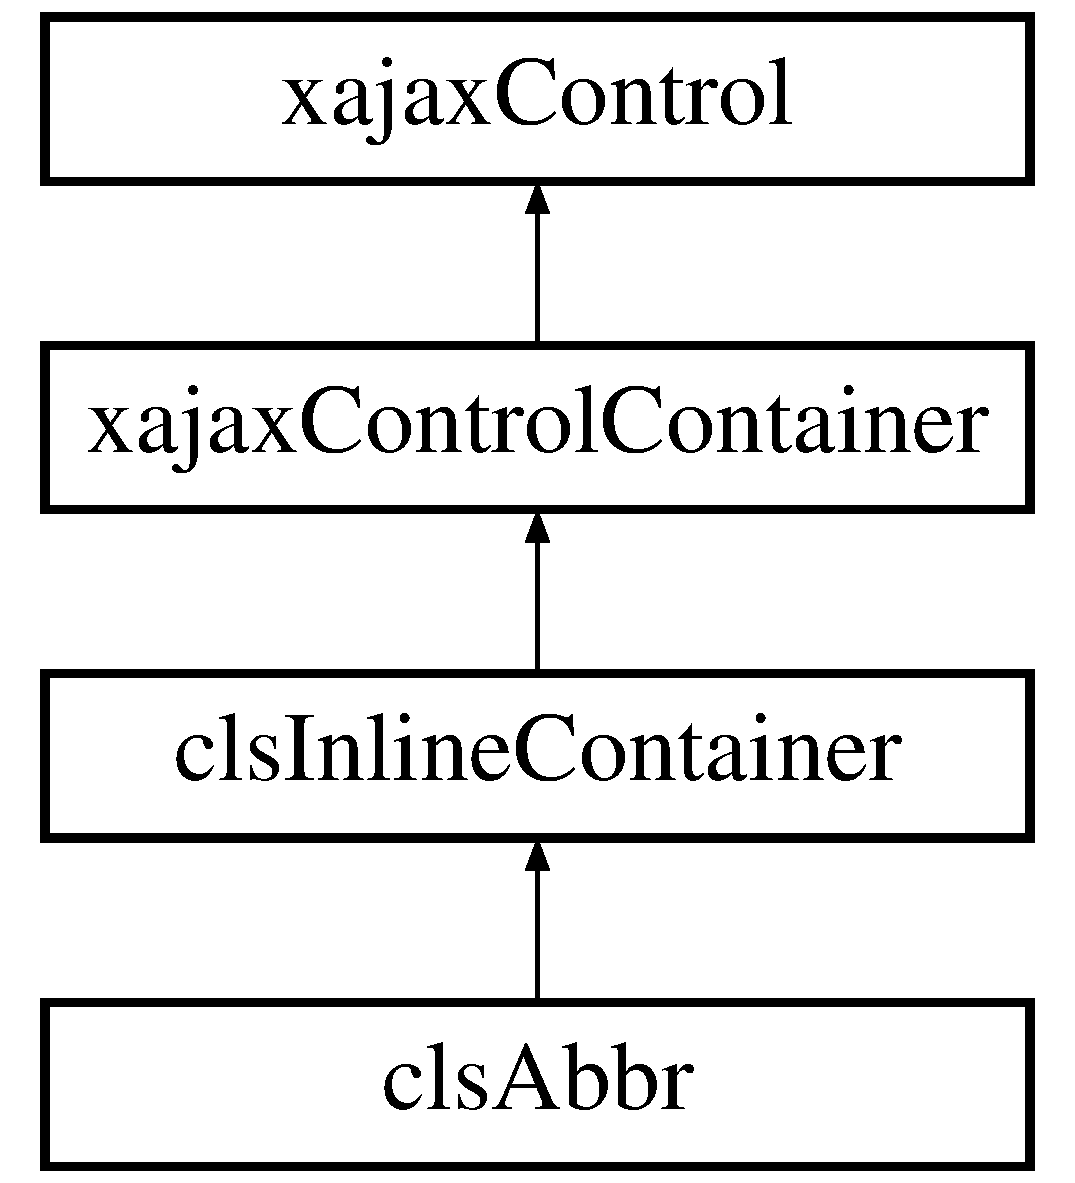
\includegraphics[height=4.000000cm]{classclsAbbr}
\end{center}
\end{figure}
\subsection*{Public Member Functions}
\begin{DoxyCompactItemize}
\item 
\hypertarget{classclsAbbr_a4d4e09b66698056d9cf60923f1f497b1}{
{\bfseries clsAbbr} (\$aConfiguration=array())}
\label{classclsAbbr_a4d4e09b66698056d9cf60923f1f497b1}

\end{DoxyCompactItemize}


\subsection{Detailed Description}


Definition at line 165 of file content.inc.php.



The documentation for this class was generated from the following file:\begin{DoxyCompactItemize}
\item 
xajax\_\-controls/content.inc.php\end{DoxyCompactItemize}

\hypertarget{classclsAcronym}{
\section{clsAcronym Class Reference}
\label{classclsAcronym}\index{clsAcronym@{clsAcronym}}
}
Inheritance diagram for clsAcronym:\begin{figure}[H]
\begin{center}
\leavevmode
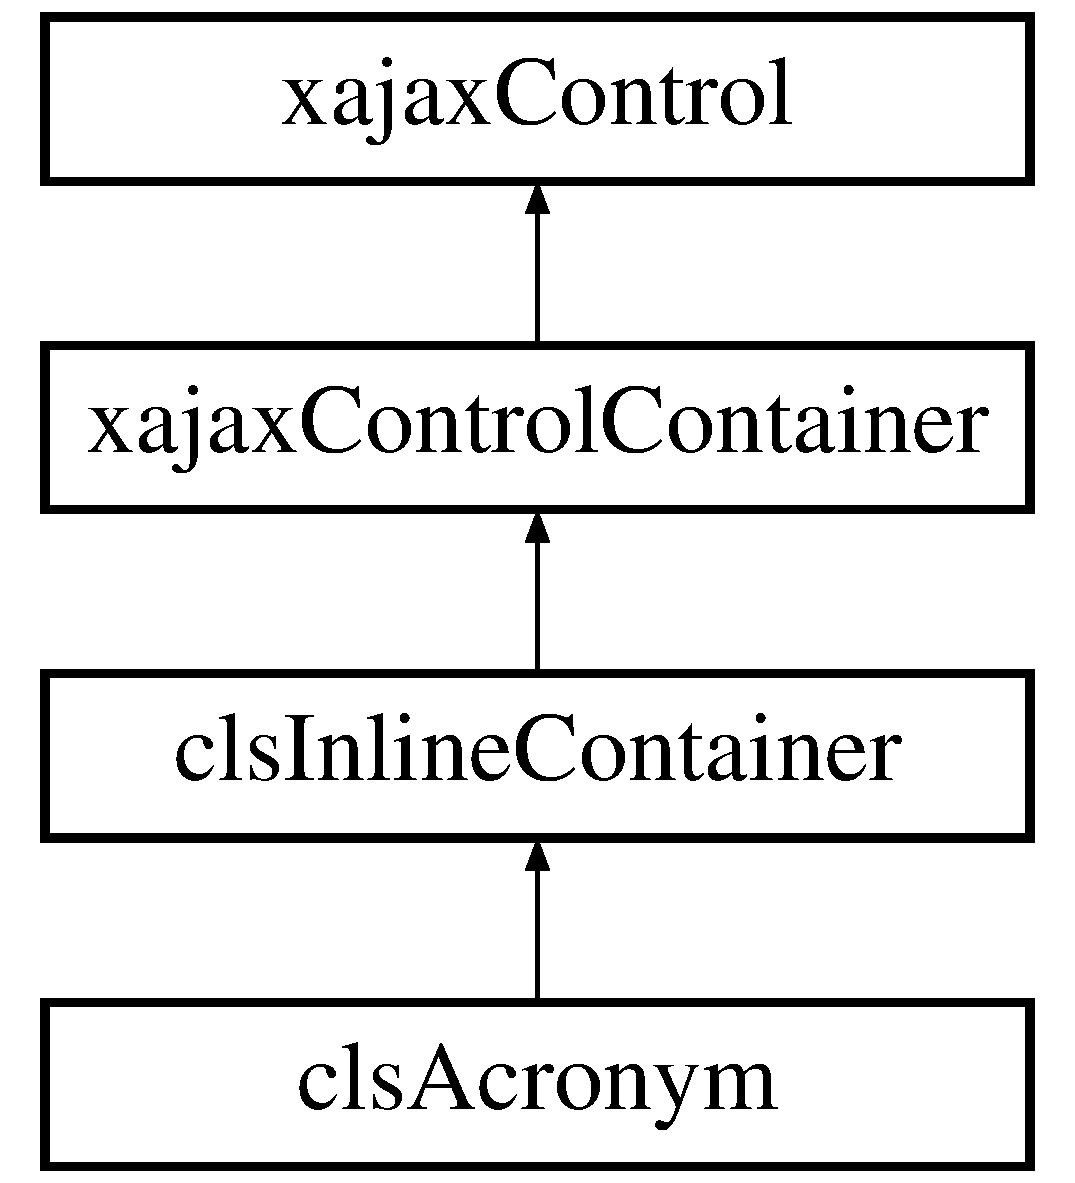
\includegraphics[height=4.000000cm]{classclsAcronym}
\end{center}
\end{figure}
\subsection*{Public Member Functions}
\begin{DoxyCompactItemize}
\item 
\hypertarget{classclsAcronym_ad3dd519cb53654c2105516435bd0eca6}{
{\bfseries clsAcronym} (\$aConfiguration=array())}
\label{classclsAcronym_ad3dd519cb53654c2105516435bd0eca6}

\end{DoxyCompactItemize}


\subsection{Detailed Description}


Definition at line 173 of file content.inc.php.



The documentation for this class was generated from the following file:\begin{DoxyCompactItemize}
\item 
xajax\_\-controls/content.inc.php\end{DoxyCompactItemize}

\hypertarget{classclsAddress}{
\section{clsAddress Class Reference}
\label{classclsAddress}\index{clsAddress@{clsAddress}}
}
Inheritance diagram for clsAddress:\begin{figure}[H]
\begin{center}
\leavevmode
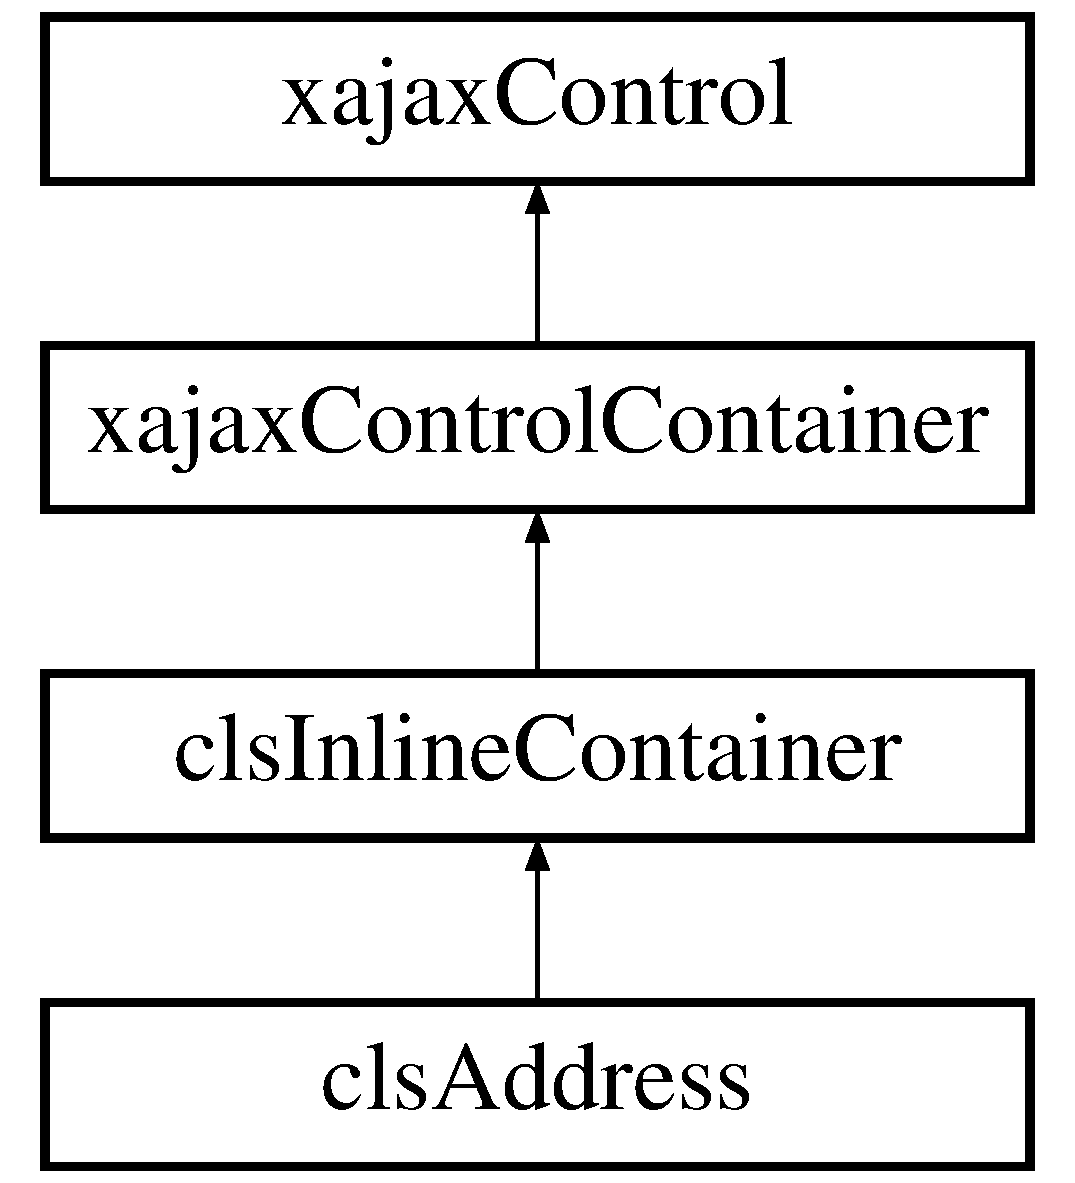
\includegraphics[height=4.000000cm]{classclsAddress}
\end{center}
\end{figure}
\subsection*{Public Member Functions}
\begin{DoxyCompactItemize}
\item 
\hypertarget{classclsAddress_a95d1c6860bfcdcec21ec229a59944c34}{
{\bfseries clsAddress} (\$aConfiguration=array())}
\label{classclsAddress_a95d1c6860bfcdcec21ec229a59944c34}

\end{DoxyCompactItemize}


\subsection{Detailed Description}


Definition at line 254 of file content.inc.php.



The documentation for this class was generated from the following file:\begin{DoxyCompactItemize}
\item 
xajax\_\-controls/content.inc.php\end{DoxyCompactItemize}

\hypertarget{classclsAnchor}{
\section{clsAnchor Class Reference}
\label{classclsAnchor}\index{clsAnchor@{clsAnchor}}
}
Inheritance diagram for clsAnchor:\begin{figure}[H]
\begin{center}
\leavevmode
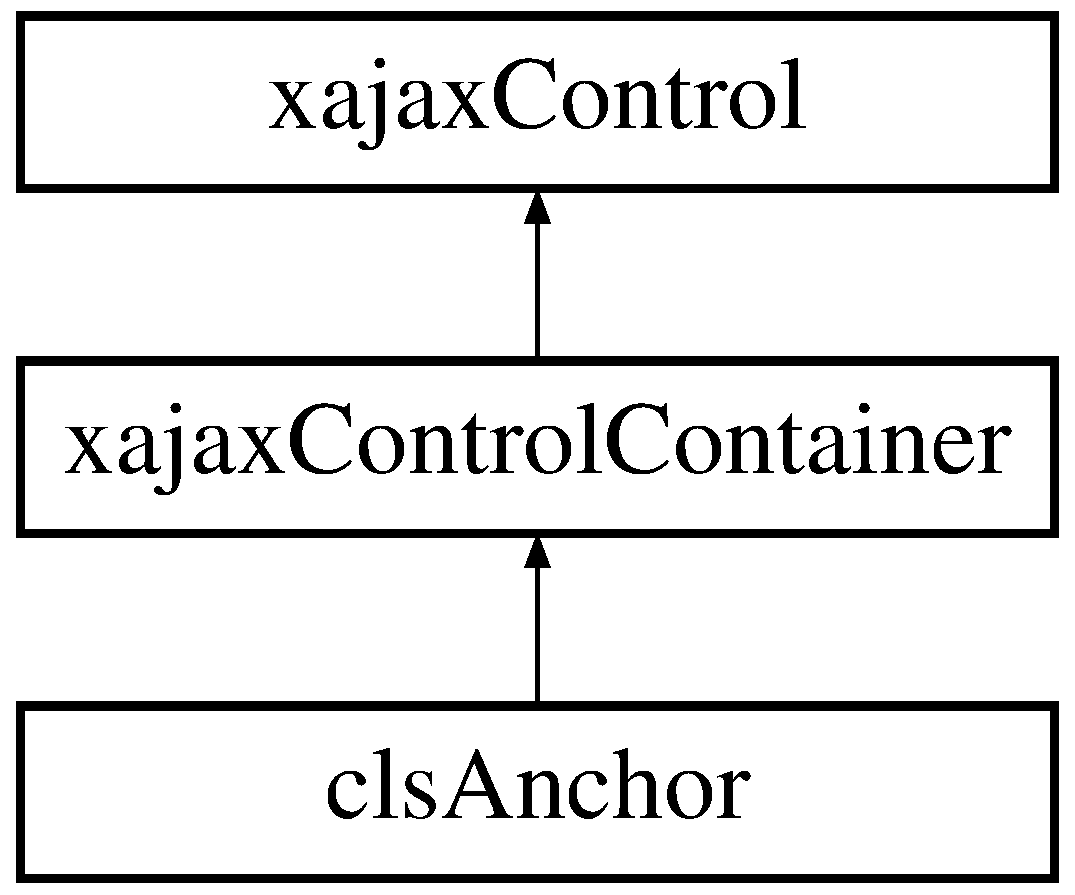
\includegraphics[height=3.000000cm]{classclsAnchor}
\end{center}
\end{figure}
\subsection*{Public Member Functions}
\begin{DoxyCompactItemize}
\item 
\hypertarget{classclsAnchor_afda4ead2464497746bb4b5386be8727e}{
{\bfseries clsAnchor} (\$aConfiguration=array())}
\label{classclsAnchor_afda4ead2464497746bb4b5386be8727e}

\item 
\hypertarget{classclsAnchor_af5fe6e3e462c93bf005aa40b868d48d7}{
{\bfseries setEvent} (\$sEvent, \&\$objRequest, \$aParameters=array(), \$sBeforeRequest='if(false== ', \$sAfterRequest=') return false; ')}
\label{classclsAnchor_af5fe6e3e462c93bf005aa40b868d48d7}

\end{DoxyCompactItemize}


\subsection{Detailed Description}


Definition at line 59 of file misc.inc.php.



The documentation for this class was generated from the following file:\begin{DoxyCompactItemize}
\item 
xajax\_\-controls/misc.inc.php\end{DoxyCompactItemize}

\hypertarget{classclsArea}{
\section{clsArea Class Reference}
\label{classclsArea}\index{clsArea@{clsArea}}
}
Inheritance diagram for clsArea:\begin{figure}[H]
\begin{center}
\leavevmode
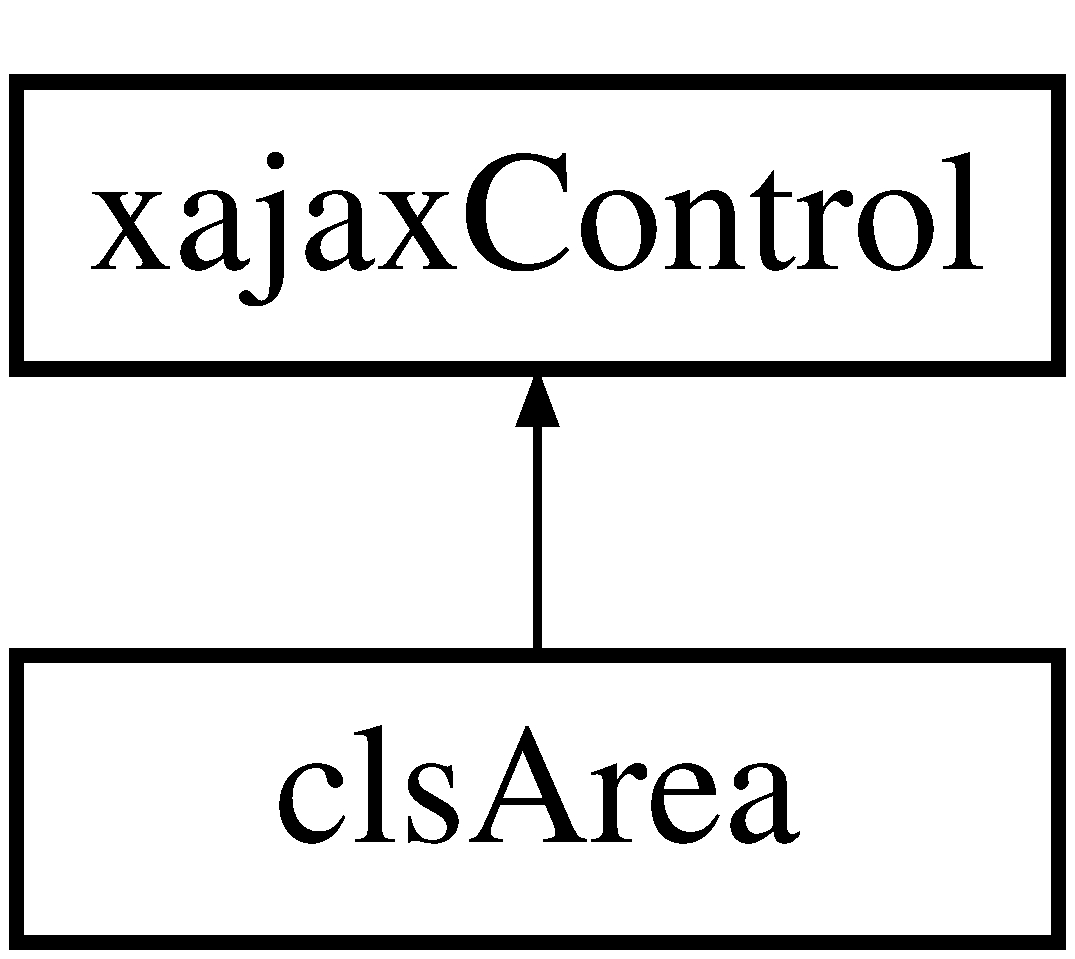
\includegraphics[height=2.000000cm]{classclsArea}
\end{center}
\end{figure}
\subsection*{Public Member Functions}
\begin{DoxyCompactItemize}
\item 
\hypertarget{classclsArea_a87097628cd924f11179a1f6975a9203f}{
{\bfseries clsArea} (\$aConfiguration=array())}
\label{classclsArea_a87097628cd924f11179a1f6975a9203f}

\end{DoxyCompactItemize}


\subsection{Detailed Description}


Definition at line 100 of file misc.inc.php.



The documentation for this class was generated from the following file:\begin{DoxyCompactItemize}
\item 
xajax\_\-controls/misc.inc.php\end{DoxyCompactItemize}

\hypertarget{classclsBase}{
\section{clsBase Class Reference}
\label{classclsBase}\index{clsBase@{clsBase}}
}
Inheritance diagram for clsBase:\begin{figure}[H]
\begin{center}
\leavevmode
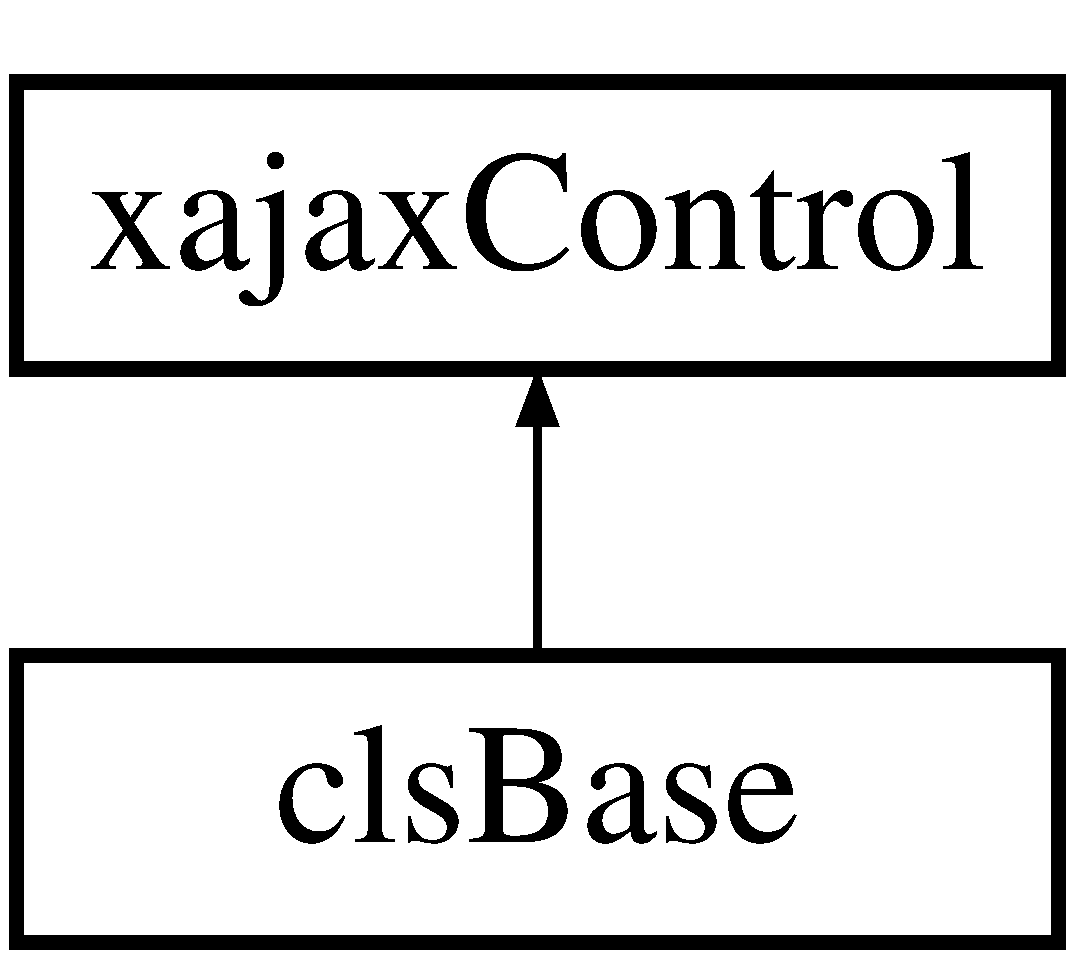
\includegraphics[height=2.000000cm]{classclsBase}
\end{center}
\end{figure}
\subsection*{Public Member Functions}
\begin{DoxyCompactItemize}
\item 
\hypertarget{classclsBase_aff15e1d4374ad0304abb55de881d7e66}{
{\bfseries clsBase} (\$aConfiguration=array())}
\label{classclsBase_aff15e1d4374ad0304abb55de881d7e66}

\end{DoxyCompactItemize}


\subsection{Detailed Description}


Definition at line 266 of file document.inc.php.



The documentation for this class was generated from the following file:\begin{DoxyCompactItemize}
\item 
xajax\_\-controls/document.inc.php\end{DoxyCompactItemize}

\hypertarget{classclsBig}{
\section{clsBig Class Reference}
\label{classclsBig}\index{clsBig@{clsBig}}
}
Inheritance diagram for clsBig:\begin{figure}[H]
\begin{center}
\leavevmode
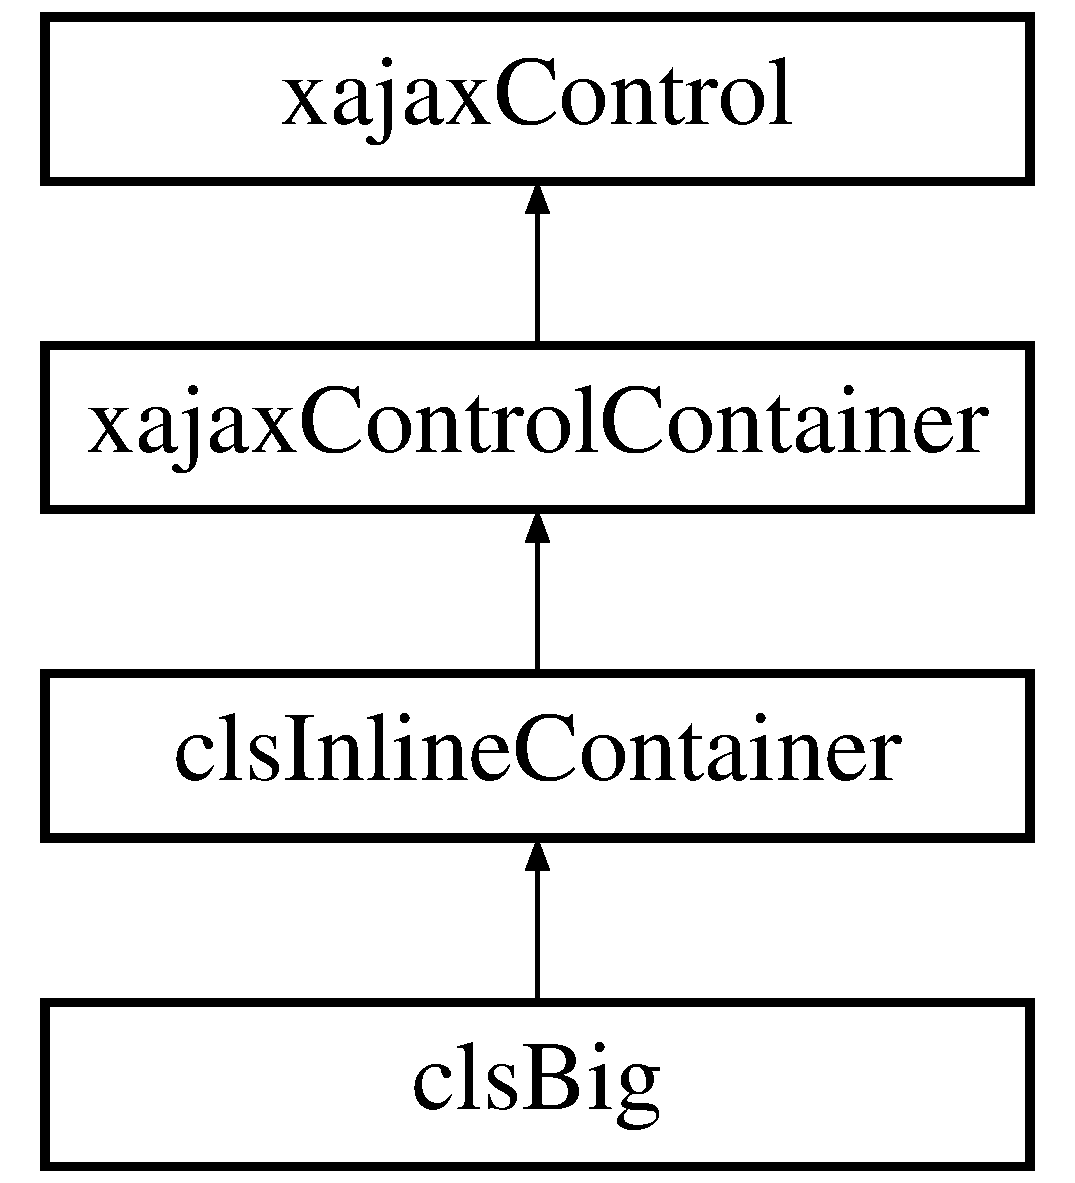
\includegraphics[height=4.000000cm]{classclsBig}
\end{center}
\end{figure}
\subsection*{Public Member Functions}
\begin{DoxyCompactItemize}
\item 
\hypertarget{classclsBig_a7aa347317bf2c17f6374541f75b1dab9}{
{\bfseries clsBig} (\$aConfiguration=array())}
\label{classclsBig_a7aa347317bf2c17f6374541f75b1dab9}

\end{DoxyCompactItemize}


\subsection{Detailed Description}


Definition at line 205 of file content.inc.php.



The documentation for this class was generated from the following file:\begin{DoxyCompactItemize}
\item 
xajax\_\-controls/content.inc.php\end{DoxyCompactItemize}

\hypertarget{classclsBlockquote}{
\section{clsBlockquote Class Reference}
\label{classclsBlockquote}\index{clsBlockquote@{clsBlockquote}}
}
Inheritance diagram for clsBlockquote:\begin{figure}[H]
\begin{center}
\leavevmode
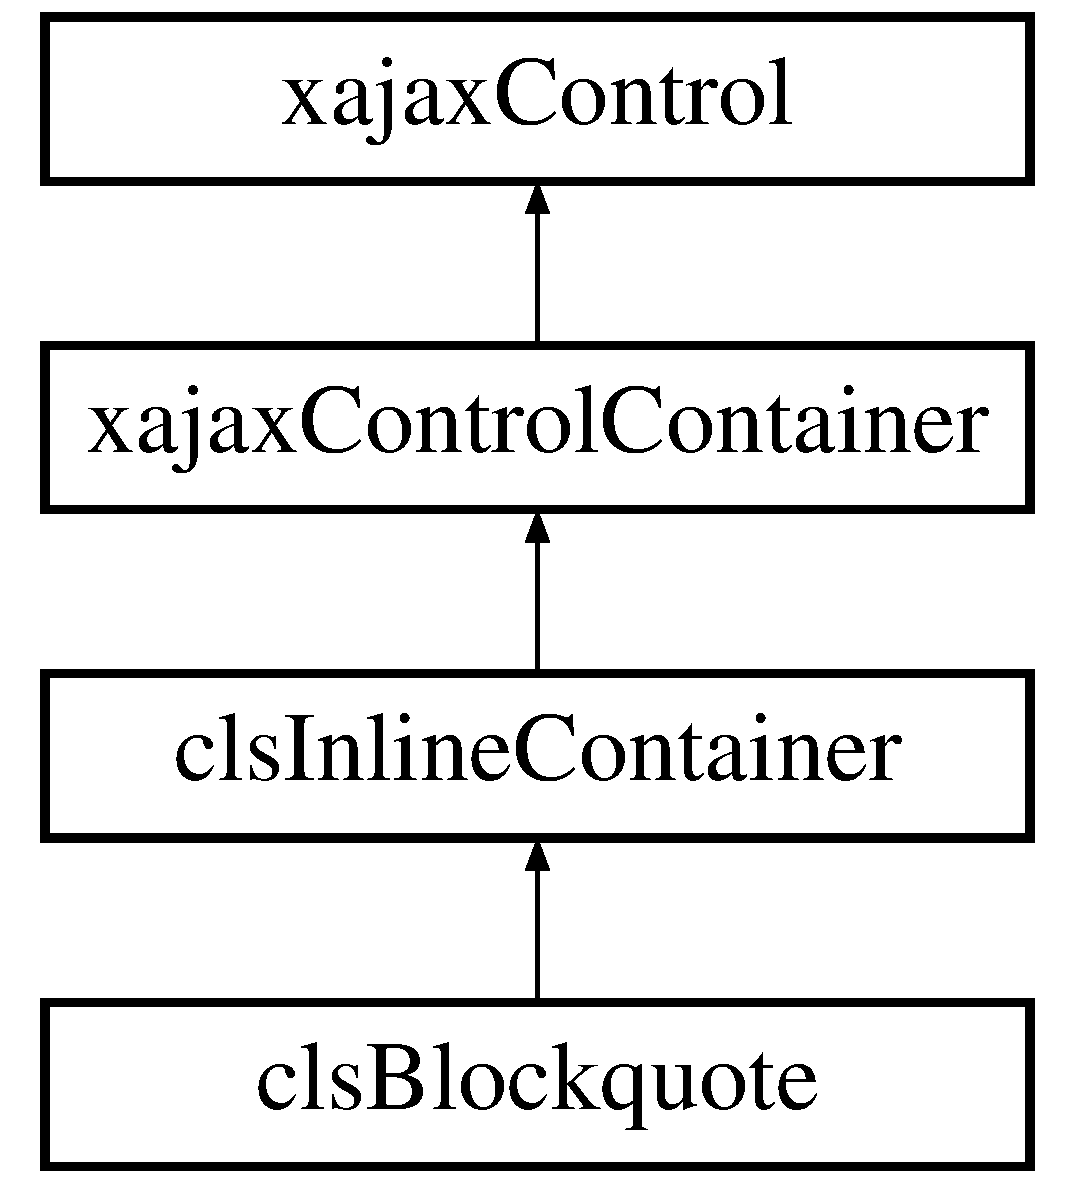
\includegraphics[height=4.000000cm]{classclsBlockquote}
\end{center}
\end{figure}
\subsection*{Public Member Functions}
\begin{DoxyCompactItemize}
\item 
\hypertarget{classclsBlockquote_abe0a6bbdad25454ca974ef9665a3d4be}{
{\bfseries clsBlockquote} (\$aConfiguration=array())}
\label{classclsBlockquote_abe0a6bbdad25454ca974ef9665a3d4be}

\end{DoxyCompactItemize}


\subsection{Detailed Description}


Definition at line 270 of file content.inc.php.



The documentation for this class was generated from the following file:\begin{DoxyCompactItemize}
\item 
xajax\_\-controls/content.inc.php\end{DoxyCompactItemize}

\hypertarget{classclsBody}{
\section{clsBody Class Reference}
\label{classclsBody}\index{clsBody@{clsBody}}
}
Inheritance diagram for clsBody:\begin{figure}[H]
\begin{center}
\leavevmode
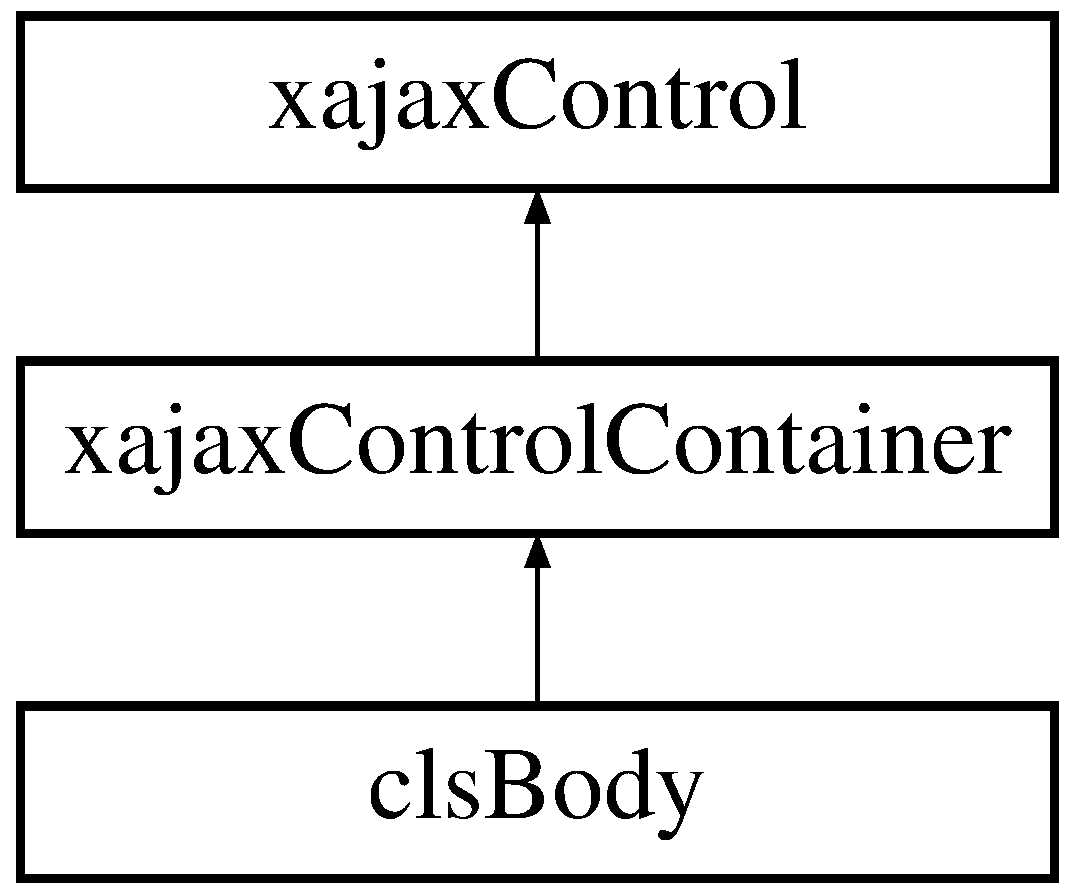
\includegraphics[height=3.000000cm]{classclsBody}
\end{center}
\end{figure}
\subsection*{Public Member Functions}
\begin{DoxyCompactItemize}
\item 
\hypertarget{classclsBody_a01d1107b3bc0c5fa9431b9359e432d35}{
{\bfseries clsBody} (\$aConfiguration=array())}
\label{classclsBody_a01d1107b3bc0c5fa9431b9359e432d35}

\end{DoxyCompactItemize}


\subsection{Detailed Description}


Definition at line 197 of file document.inc.php.



The documentation for this class was generated from the following file:\begin{DoxyCompactItemize}
\item 
xajax\_\-controls/document.inc.php\end{DoxyCompactItemize}

\hypertarget{classclsBold}{
\section{clsBold Class Reference}
\label{classclsBold}\index{clsBold@{clsBold}}
}
Inheritance diagram for clsBold:\begin{figure}[H]
\begin{center}
\leavevmode
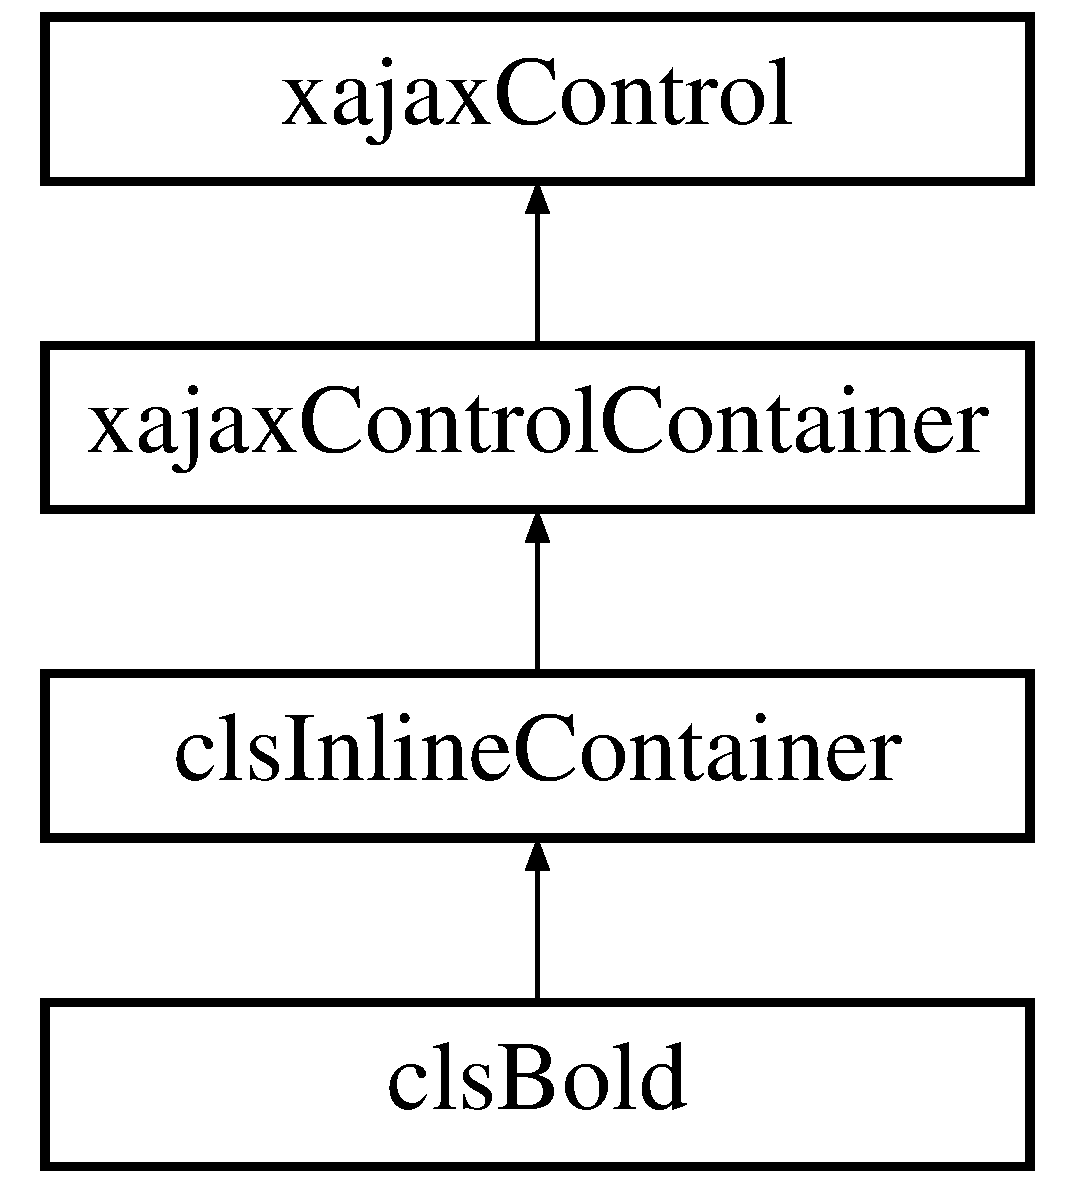
\includegraphics[height=4.000000cm]{classclsBold}
\end{center}
\end{figure}
\subsection*{Public Member Functions}
\begin{DoxyCompactItemize}
\item 
\hypertarget{classclsBold_a2358aad878e20edd0db792ae8d1bfb99}{
{\bfseries clsBold} (\$aConfiguration=array())}
\label{classclsBold_a2358aad878e20edd0db792ae8d1bfb99}

\end{DoxyCompactItemize}


\subsection{Detailed Description}


Definition at line 197 of file content.inc.php.



The documentation for this class was generated from the following file:\begin{DoxyCompactItemize}
\item 
xajax\_\-controls/content.inc.php\end{DoxyCompactItemize}

\hypertarget{classclsBr}{
\section{clsBr Class Reference}
\label{classclsBr}\index{clsBr@{clsBr}}
}
Inheritance diagram for clsBr:\begin{figure}[H]
\begin{center}
\leavevmode
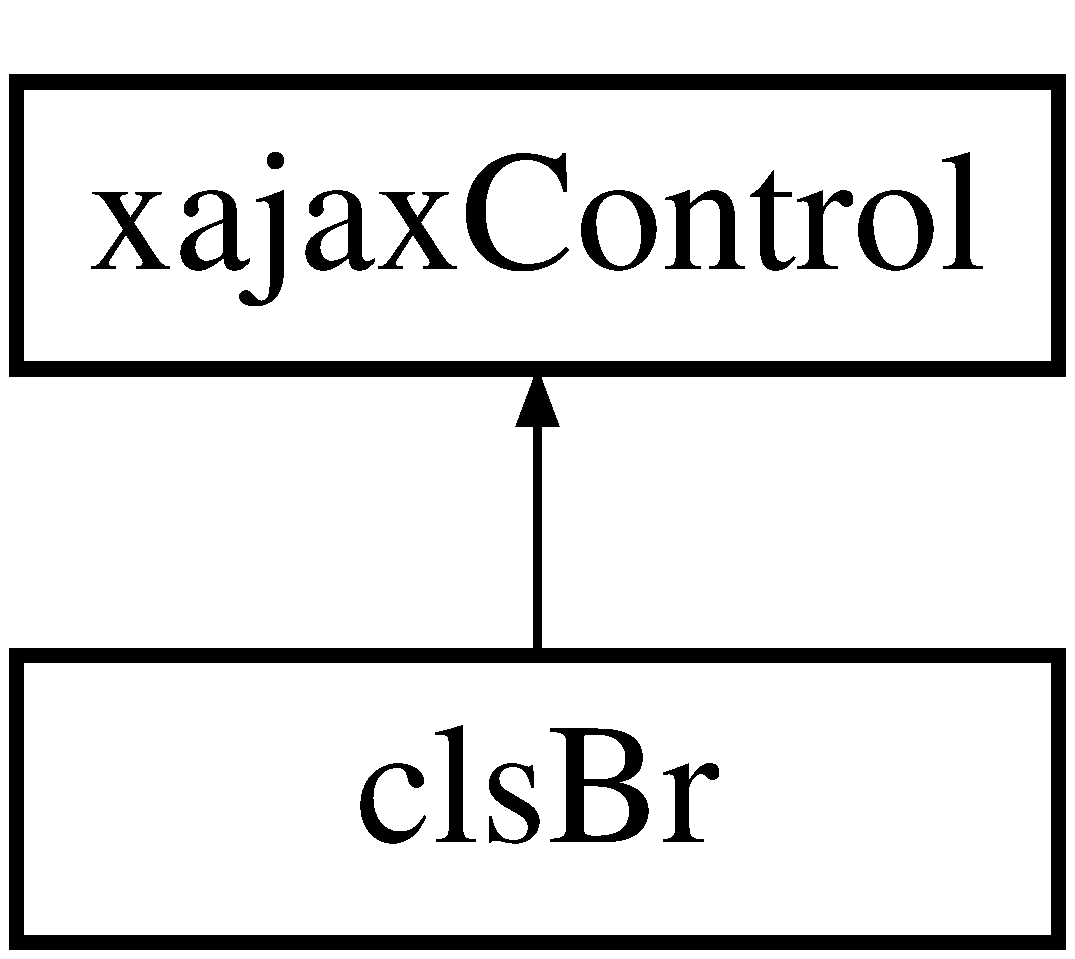
\includegraphics[height=2.000000cm]{classclsBr}
\end{center}
\end{figure}
\subsection*{Public Member Functions}
\begin{DoxyCompactItemize}
\item 
\hypertarget{classclsBr_ac6802a9e1bd34d7e9aa6d31e7e716f37}{
{\bfseries clsBr} (\$aConfiguration=array())}
\label{classclsBr_ac6802a9e1bd34d7e9aa6d31e7e716f37}

\end{DoxyCompactItemize}


\subsection{Detailed Description}


Definition at line 52 of file content.inc.php.



The documentation for this class was generated from the following file:\begin{DoxyCompactItemize}
\item 
xajax\_\-controls/content.inc.php\end{DoxyCompactItemize}

\hypertarget{classclsButton}{
\section{clsButton Class Reference}
\label{classclsButton}\index{clsButton@{clsButton}}
}
Inheritance diagram for clsButton:\begin{figure}[H]
\begin{center}
\leavevmode
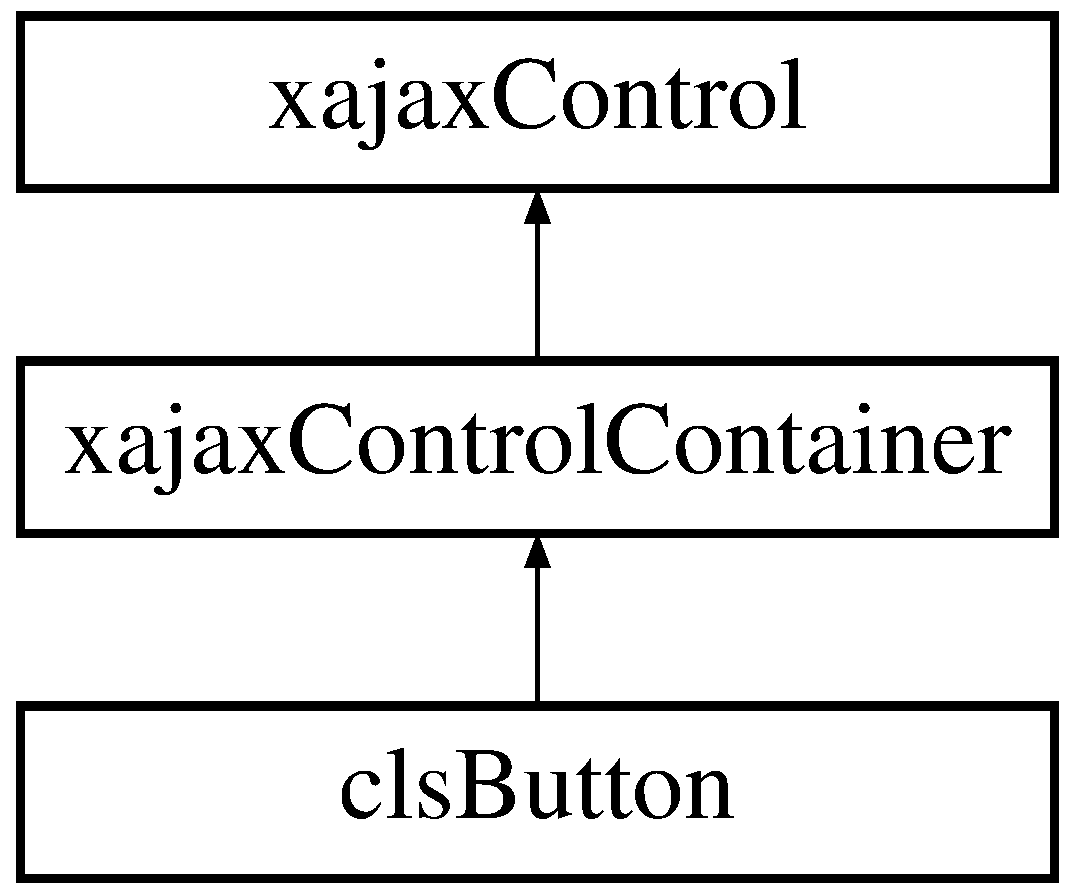
\includegraphics[height=3.000000cm]{classclsButton}
\end{center}
\end{figure}
\subsection*{Public Member Functions}
\begin{DoxyCompactItemize}
\item 
\hypertarget{classclsButton_af1ece6d106354759d47923e99f22aa8f}{
{\bfseries clsButton} (\$aConfiguration=array())}
\label{classclsButton_af1ece6d106354759d47923e99f22aa8f}

\end{DoxyCompactItemize}


\subsection{Detailed Description}


Definition at line 90 of file misc.inc.php.



The documentation for this class was generated from the following file:\begin{DoxyCompactItemize}
\item 
xajax\_\-controls/misc.inc.php\end{DoxyCompactItemize}

\hypertarget{classclsCaption}{
\section{clsCaption Class Reference}
\label{classclsCaption}\index{clsCaption@{clsCaption}}
}
Inheritance diagram for clsCaption:\begin{figure}[H]
\begin{center}
\leavevmode
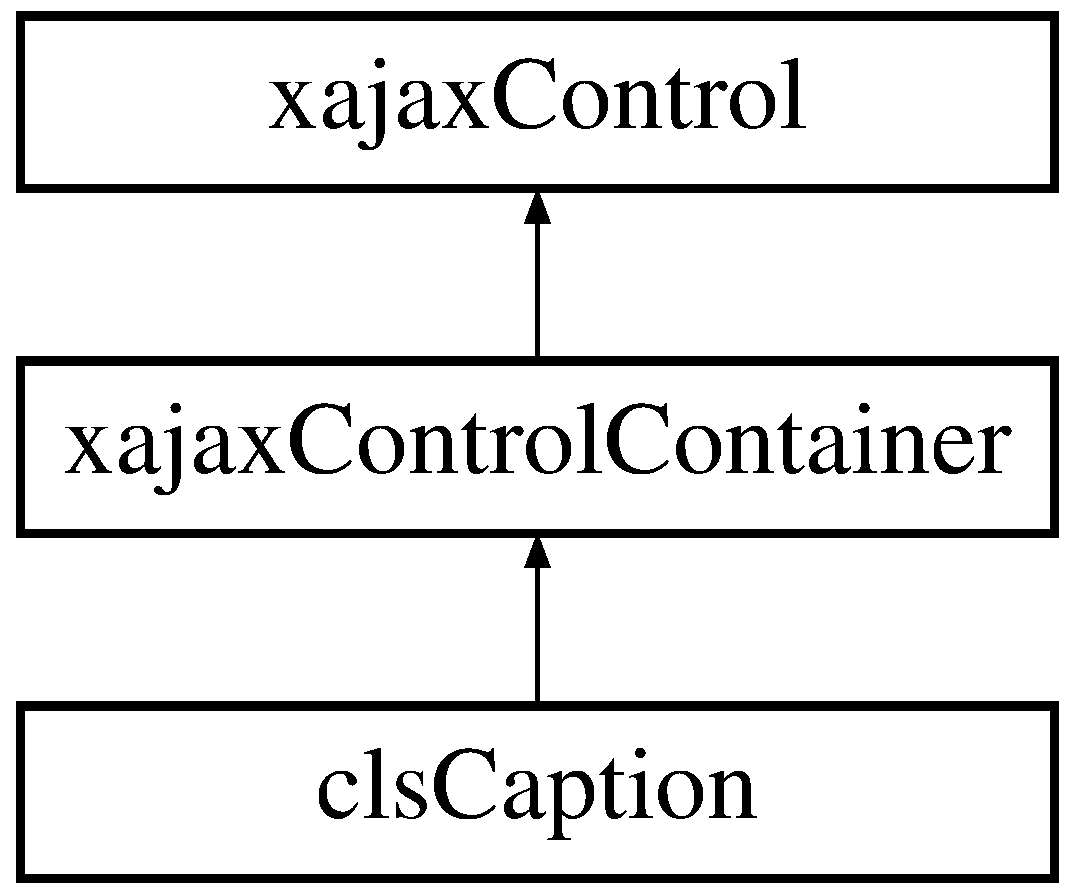
\includegraphics[height=3.000000cm]{classclsCaption}
\end{center}
\end{figure}
\subsection*{Public Member Functions}
\begin{DoxyCompactItemize}
\item 
\hypertarget{classclsCaption_a4742139d35099b8f7f31eacb121615c1}{
{\bfseries clsCaption} (\$aConfiguration=array())}
\label{classclsCaption_a4742139d35099b8f7f31eacb121615c1}

\end{DoxyCompactItemize}


\subsection{Detailed Description}


Definition at line 408 of file group.inc.php.



The documentation for this class was generated from the following file:\begin{DoxyCompactItemize}
\item 
xajax\_\-controls/group.inc.php\end{DoxyCompactItemize}

\hypertarget{classclsCite}{
\section{clsCite Class Reference}
\label{classclsCite}\index{clsCite@{clsCite}}
}
Inheritance diagram for clsCite:\begin{figure}[H]
\begin{center}
\leavevmode
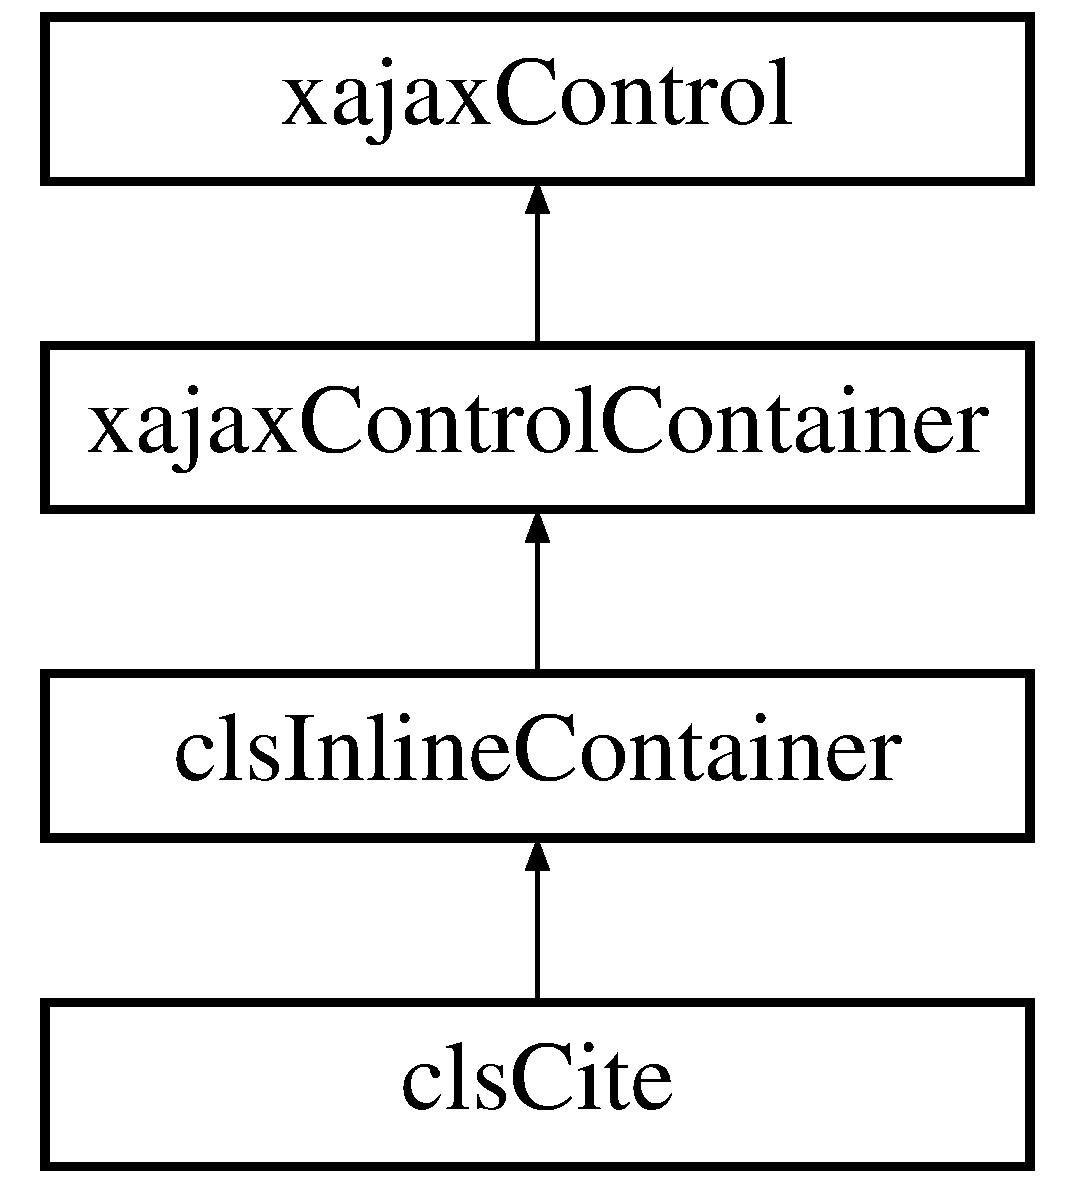
\includegraphics[height=4.000000cm]{classclsCite}
\end{center}
\end{figure}
\subsection*{Public Member Functions}
\begin{DoxyCompactItemize}
\item 
\hypertarget{classclsCite_a14b2e3135e616318937f8d86cddea132}{
{\bfseries clsCite} (\$aConfiguration=array())}
\label{classclsCite_a14b2e3135e616318937f8d86cddea132}

\end{DoxyCompactItemize}


\subsection{Detailed Description}


Definition at line 117 of file content.inc.php.



The documentation for this class was generated from the following file:\begin{DoxyCompactItemize}
\item 
xajax\_\-controls/content.inc.php\end{DoxyCompactItemize}

\hypertarget{classclsCode}{
\section{clsCode Class Reference}
\label{classclsCode}\index{clsCode@{clsCode}}
}
Inheritance diagram for clsCode:\begin{figure}[H]
\begin{center}
\leavevmode
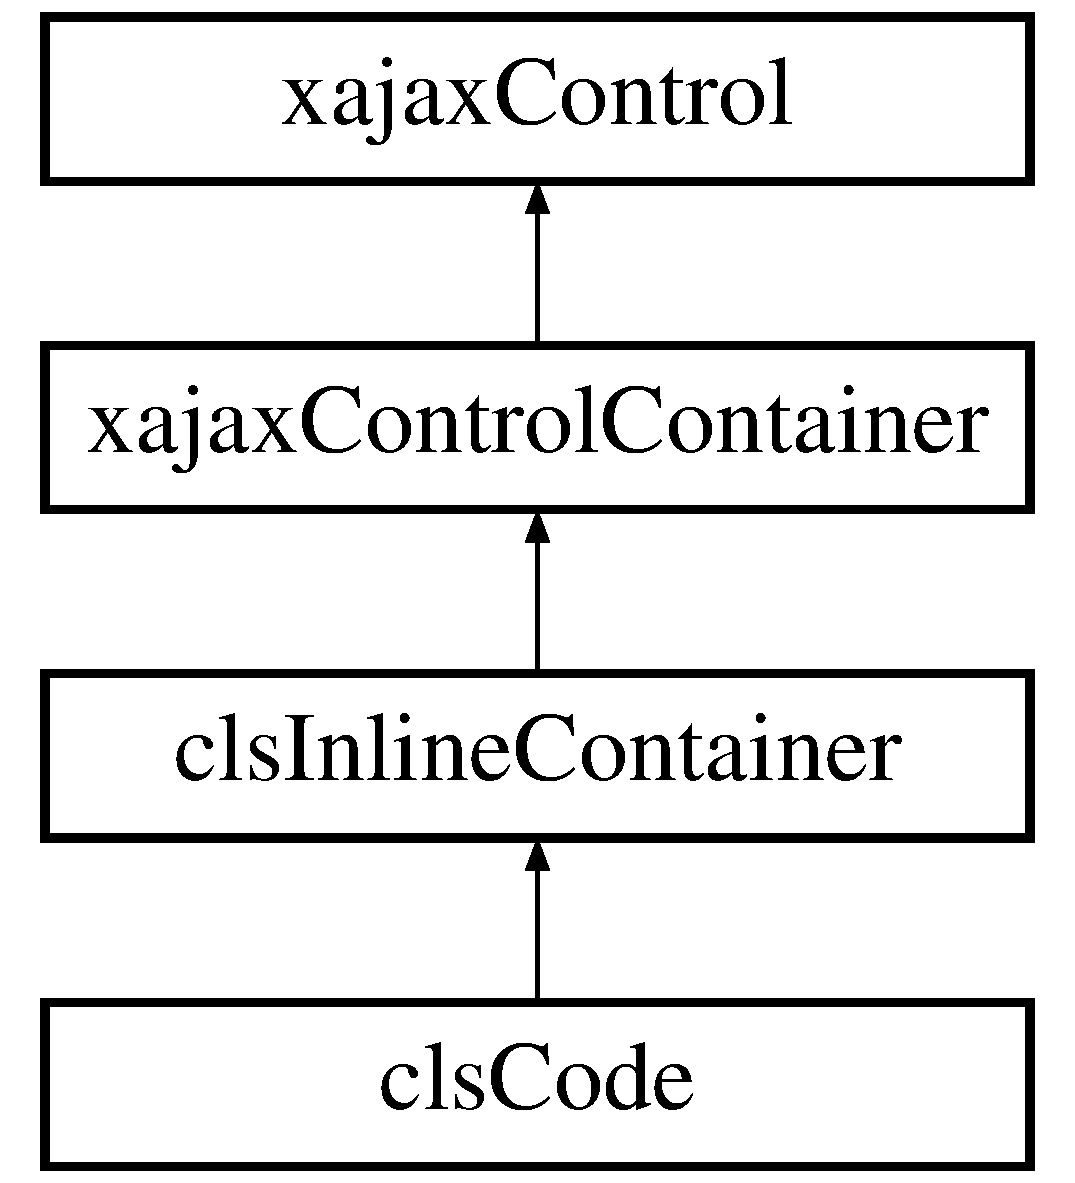
\includegraphics[height=4.000000cm]{classclsCode}
\end{center}
\end{figure}
\subsection*{Public Member Functions}
\begin{DoxyCompactItemize}
\item 
\hypertarget{classclsCode_a27ec002d6027b6fc7f413042ddf63825}{
{\bfseries clsCode} (\$aConfiguration=array())}
\label{classclsCode_a27ec002d6027b6fc7f413042ddf63825}

\end{DoxyCompactItemize}


\subsection{Detailed Description}


Definition at line 133 of file content.inc.php.



The documentation for this class was generated from the following file:\begin{DoxyCompactItemize}
\item 
xajax\_\-controls/content.inc.php\end{DoxyCompactItemize}

\hypertarget{classclsCol}{
\section{clsCol Class Reference}
\label{classclsCol}\index{clsCol@{clsCol}}
}
Inheritance diagram for clsCol:\begin{figure}[H]
\begin{center}
\leavevmode
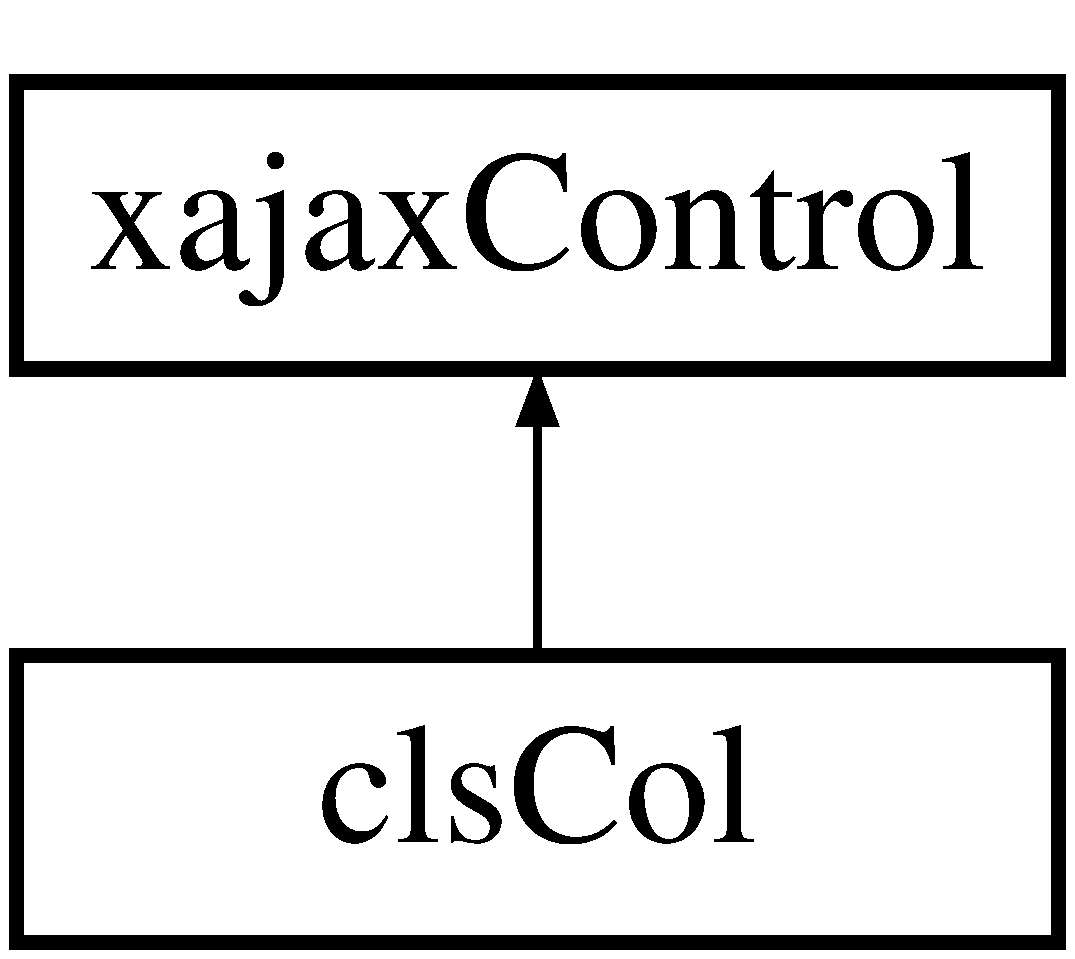
\includegraphics[height=2.000000cm]{classclsCol}
\end{center}
\end{figure}
\subsection*{Public Member Functions}
\begin{DoxyCompactItemize}
\item 
\hypertarget{classclsCol_a98d216704230af20a7282fc28028a8d4}{
{\bfseries clsCol} (\$aConfiguration=array())}
\label{classclsCol_a98d216704230af20a7282fc28028a8d4}

\end{DoxyCompactItemize}


\subsection{Detailed Description}


Definition at line 429 of file group.inc.php.



The documentation for this class was generated from the following file:\begin{DoxyCompactItemize}
\item 
xajax\_\-controls/group.inc.php\end{DoxyCompactItemize}

\hypertarget{classclsColgroup}{
\section{clsColgroup Class Reference}
\label{classclsColgroup}\index{clsColgroup@{clsColgroup}}
}
Inheritance diagram for clsColgroup:\begin{figure}[H]
\begin{center}
\leavevmode
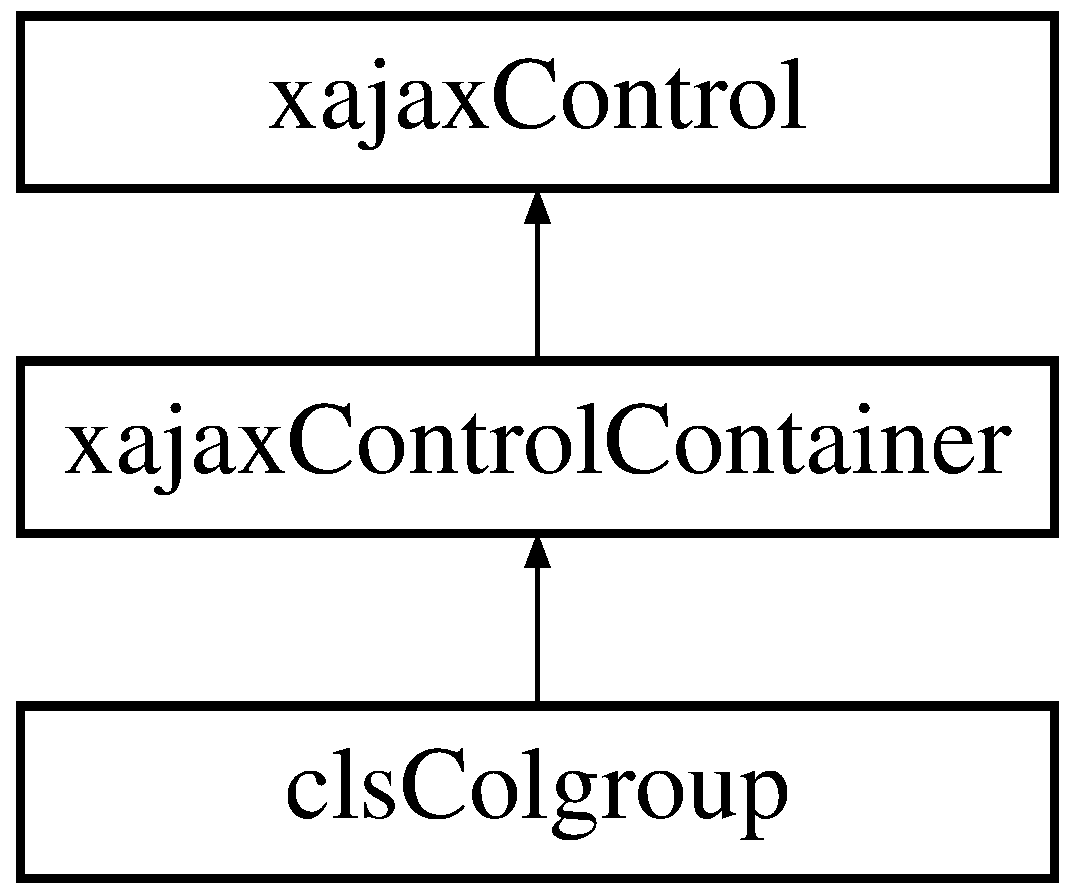
\includegraphics[height=3.000000cm]{classclsColgroup}
\end{center}
\end{figure}
\subsection*{Public Member Functions}
\begin{DoxyCompactItemize}
\item 
\hypertarget{classclsColgroup_afbf4f9602160ea4cae4d0d941bee06c9}{
{\bfseries clsColgroup} (\$aConfiguration=array())}
\label{classclsColgroup_afbf4f9602160ea4cae4d0d941bee06c9}

\end{DoxyCompactItemize}


\subsection{Detailed Description}


Definition at line 418 of file group.inc.php.



The documentation for this class was generated from the following file:\begin{DoxyCompactItemize}
\item 
xajax\_\-controls/group.inc.php\end{DoxyCompactItemize}

\hypertarget{classclsContext}{
\section{clsContext Class Reference}
\label{classclsContext}\index{clsContext@{clsContext}}
}
\subsection*{Public Member Functions}
\begin{DoxyCompactItemize}
\item 
\hypertarget{classclsContext_a0b388254bf1481854c7d463c3f3cafcc}{
{\bfseries begin} (\$iframe)}
\label{classclsContext_a0b388254bf1481854c7d463c3f3cafcc}

\item 
\hypertarget{classclsContext_a43bab5d06b8186e66c843069d3810738}{
{\bfseries end} ()}
\label{classclsContext_a43bab5d06b8186e66c843069d3810738}

\end{DoxyCompactItemize}


\subsection{Detailed Description}


Definition at line 21 of file iframe.php.



The documentation for this class was generated from the following file:\begin{DoxyCompactItemize}
\item 
tests/suite/iframe.php\end{DoxyCompactItemize}

\hypertarget{classclsDd}{
\section{clsDd Class Reference}
\label{classclsDd}\index{clsDd@{clsDd}}
}
Inheritance diagram for clsDd:\begin{figure}[H]
\begin{center}
\leavevmode
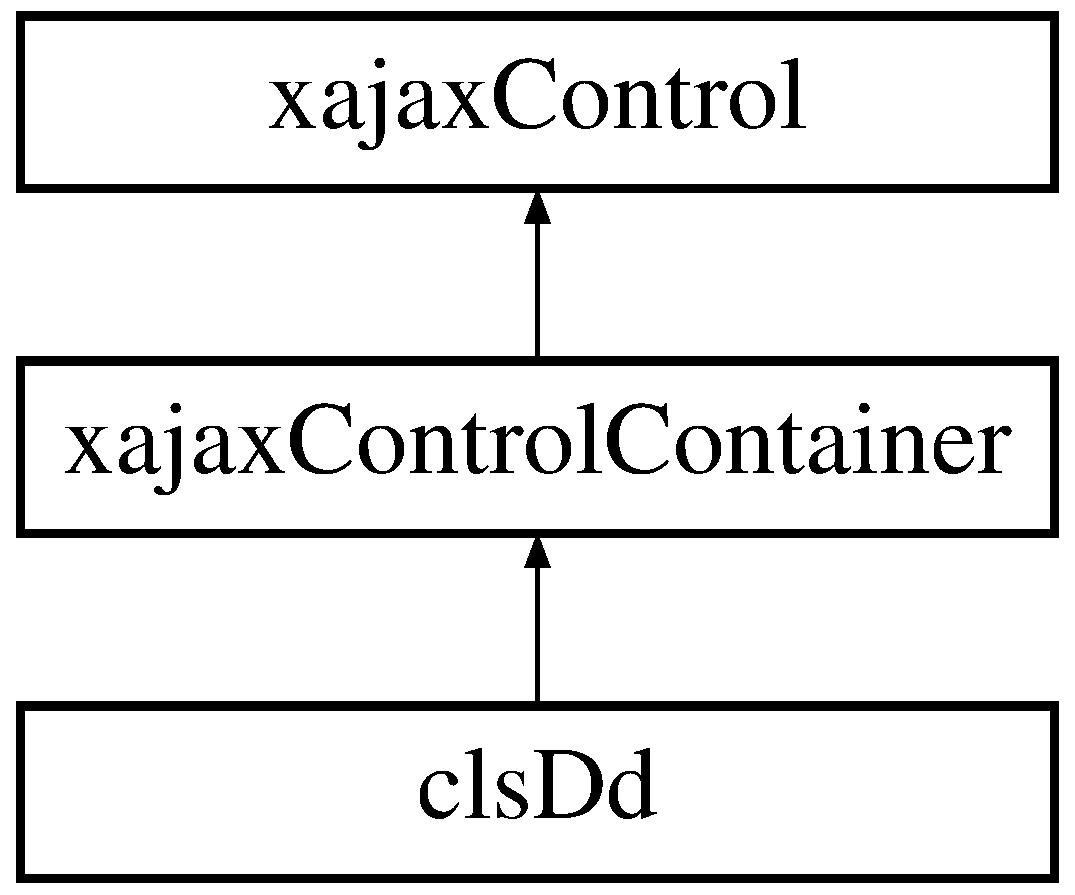
\includegraphics[height=3.000000cm]{classclsDd}
\end{center}
\end{figure}
\subsection*{Public Member Functions}
\begin{DoxyCompactItemize}
\item 
\hypertarget{classclsDd_a6bcc55f409decbcfbf29c28af982a9e9}{
{\bfseries clsDd} (\$aConfiguration=array())}
\label{classclsDd_a6bcc55f409decbcfbf29c28af982a9e9}

\end{DoxyCompactItemize}


\subsection{Detailed Description}


Definition at line 131 of file group.inc.php.



The documentation for this class was generated from the following file:\begin{DoxyCompactItemize}
\item 
xajax\_\-controls/group.inc.php\end{DoxyCompactItemize}

\hypertarget{classclsDel}{
\section{clsDel Class Reference}
\label{classclsDel}\index{clsDel@{clsDel}}
}
Inheritance diagram for clsDel:\begin{figure}[H]
\begin{center}
\leavevmode
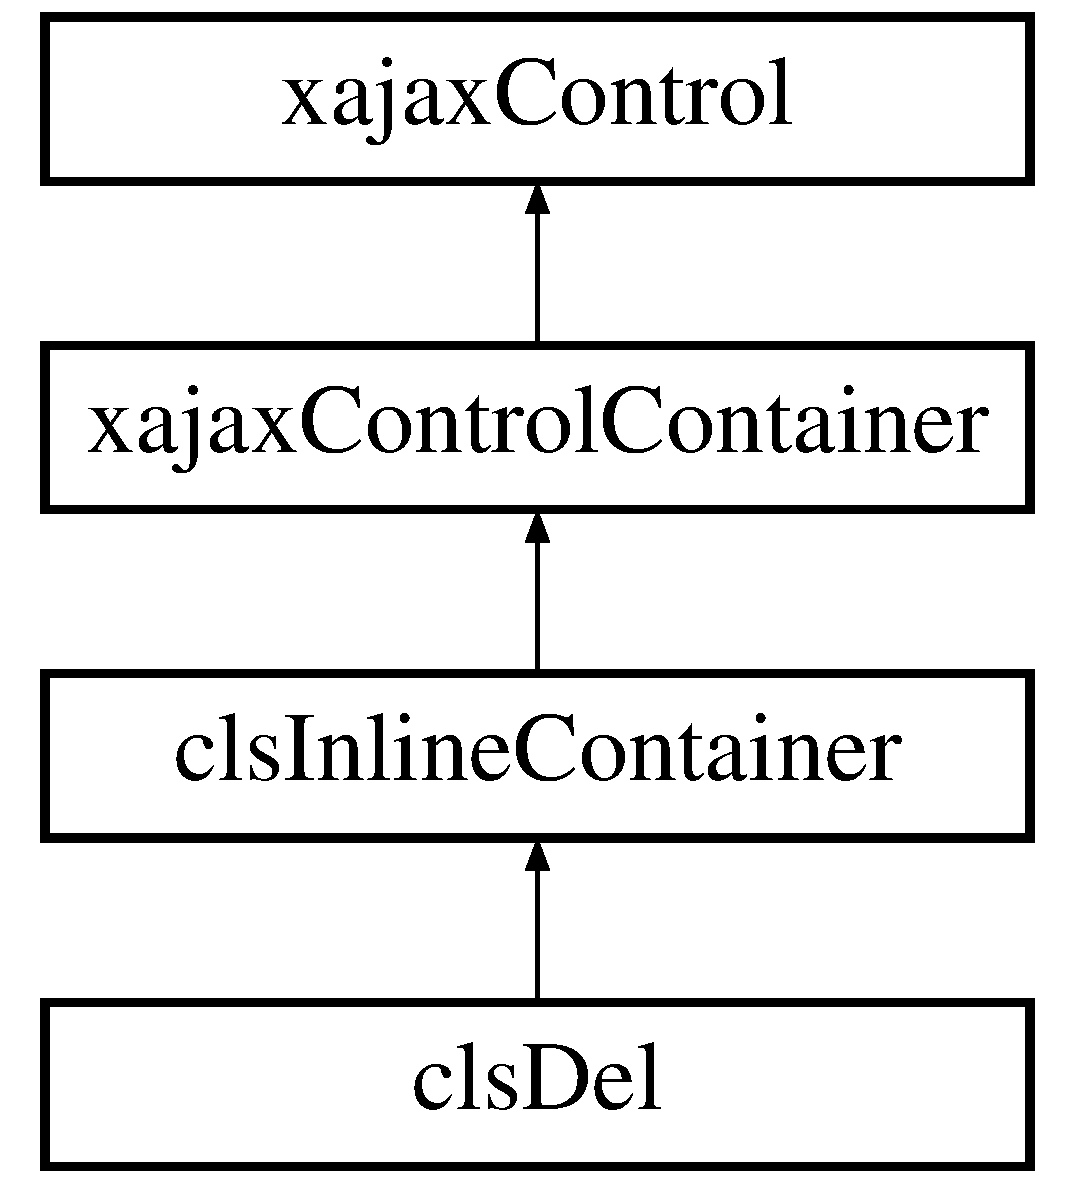
\includegraphics[height=4.000000cm]{classclsDel}
\end{center}
\end{figure}
\subsection*{Public Member Functions}
\begin{DoxyCompactItemize}
\item 
\hypertarget{classclsDel_ab198d7892032e0d1ff7fa97d97fc8ef8}{
{\bfseries clsDel} (\$aConfiguration=array())}
\label{classclsDel_ab198d7892032e0d1ff7fa97d97fc8ef8}

\end{DoxyCompactItemize}


\subsection{Detailed Description}


Definition at line 230 of file content.inc.php.



The documentation for this class was generated from the following file:\begin{DoxyCompactItemize}
\item 
xajax\_\-controls/content.inc.php\end{DoxyCompactItemize}

\hypertarget{classclsDfn}{
\section{clsDfn Class Reference}
\label{classclsDfn}\index{clsDfn@{clsDfn}}
}
Inheritance diagram for clsDfn:\begin{figure}[H]
\begin{center}
\leavevmode
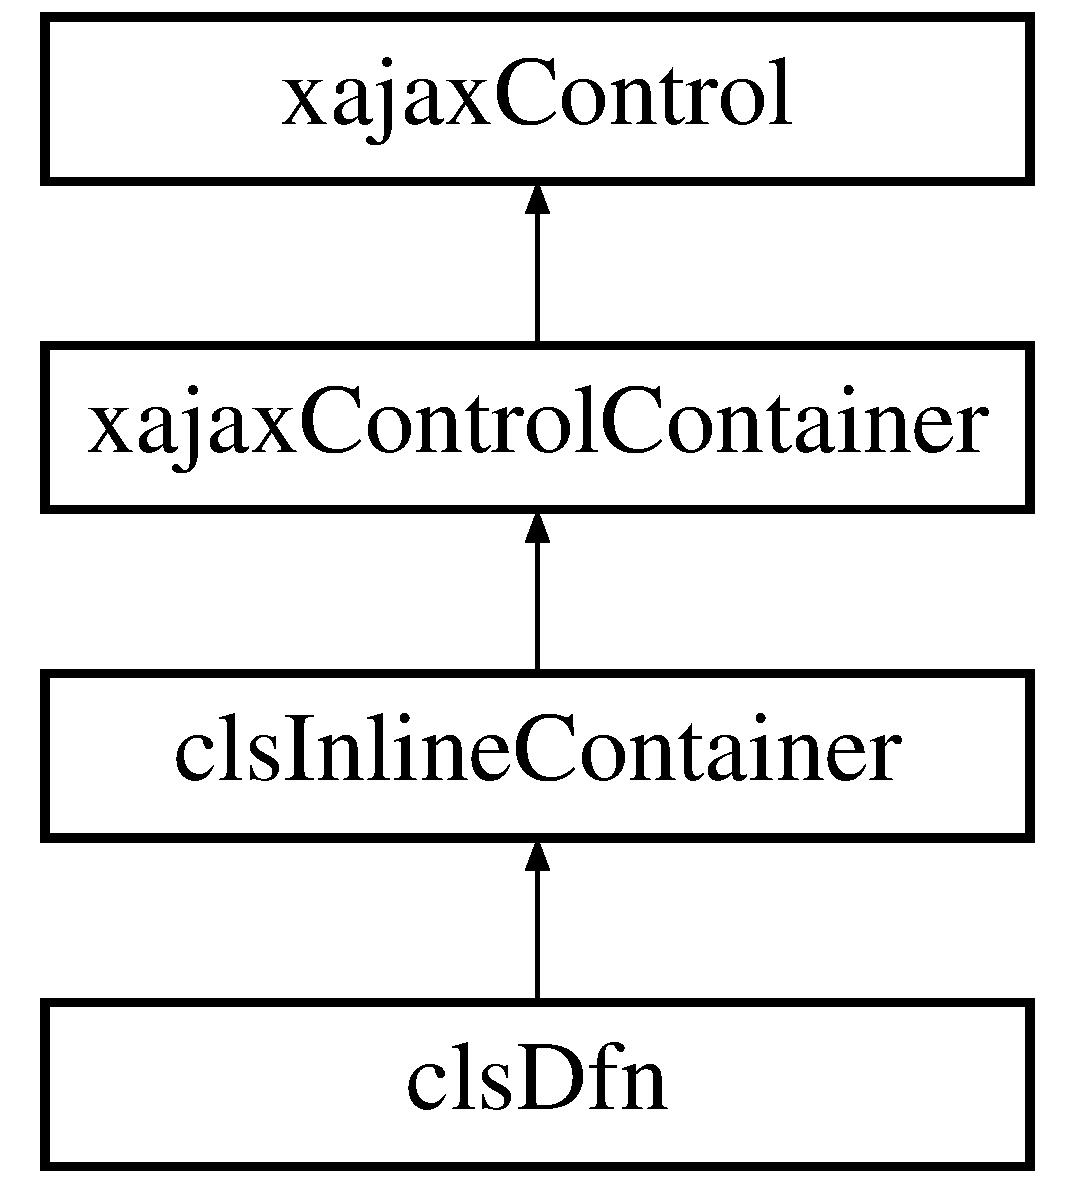
\includegraphics[height=4.000000cm]{classclsDfn}
\end{center}
\end{figure}
\subsection*{Public Member Functions}
\begin{DoxyCompactItemize}
\item 
\hypertarget{classclsDfn_af845eb0a3ed2bc0da59cdc1b02692001}{
{\bfseries clsDfn} (\$aConfiguration=array())}
\label{classclsDfn_af845eb0a3ed2bc0da59cdc1b02692001}

\end{DoxyCompactItemize}


\subsection{Detailed Description}


Definition at line 125 of file content.inc.php.



The documentation for this class was generated from the following file:\begin{DoxyCompactItemize}
\item 
xajax\_\-controls/content.inc.php\end{DoxyCompactItemize}

\hypertarget{classclsDiv}{
\section{clsDiv Class Reference}
\label{classclsDiv}\index{clsDiv@{clsDiv}}
}
Inheritance diagram for clsDiv:\begin{figure}[H]
\begin{center}
\leavevmode
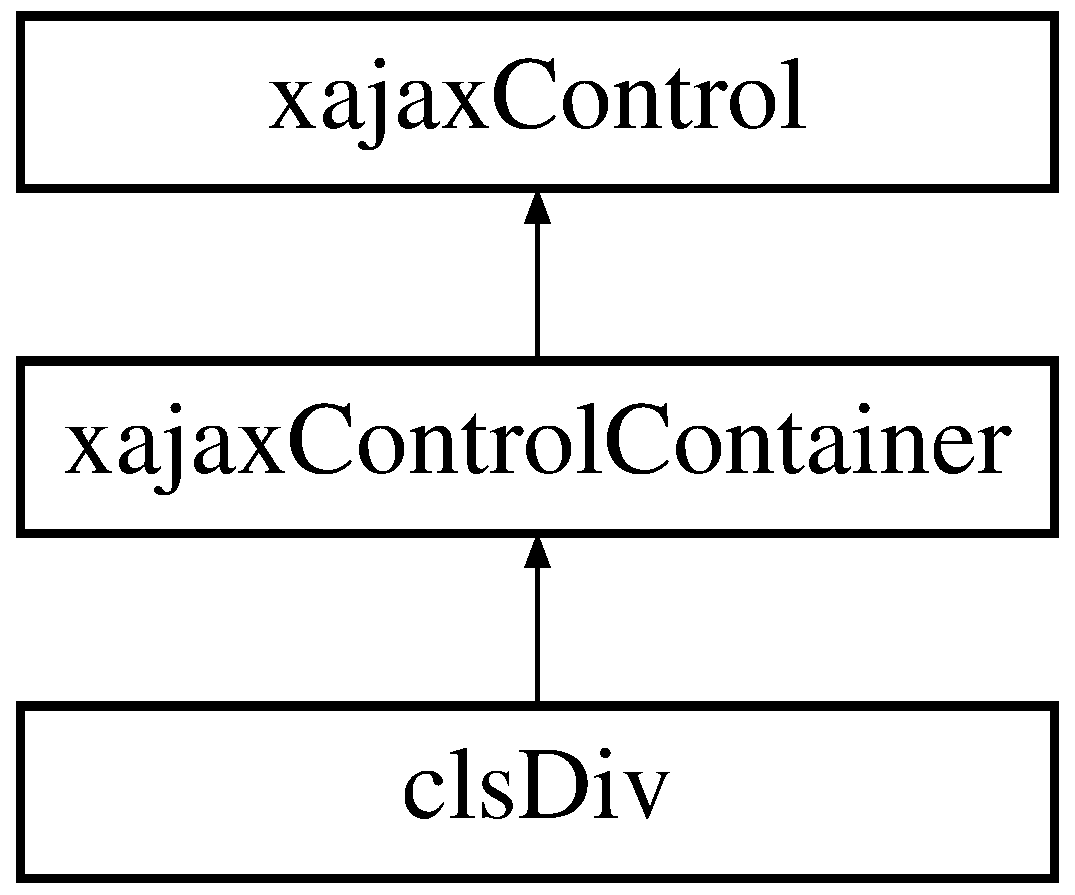
\includegraphics[height=3.000000cm]{classclsDiv}
\end{center}
\end{figure}
\subsection*{Public Member Functions}
\begin{DoxyCompactItemize}
\item 
\hypertarget{classclsDiv_a58289f447cff1fe2a92e6fc22fde5690}{
{\bfseries clsDiv} (\$aConfiguration=array())}
\label{classclsDiv_a58289f447cff1fe2a92e6fc22fde5690}

\end{DoxyCompactItemize}


\subsection{Detailed Description}


Definition at line 29 of file structure.inc.php.



The documentation for this class was generated from the following file:\begin{DoxyCompactItemize}
\item 
xajax\_\-controls/structure.inc.php\end{DoxyCompactItemize}

\hypertarget{classclsDl}{
\section{clsDl Class Reference}
\label{classclsDl}\index{clsDl@{clsDl}}
}
Inheritance diagram for clsDl:\begin{figure}[H]
\begin{center}
\leavevmode
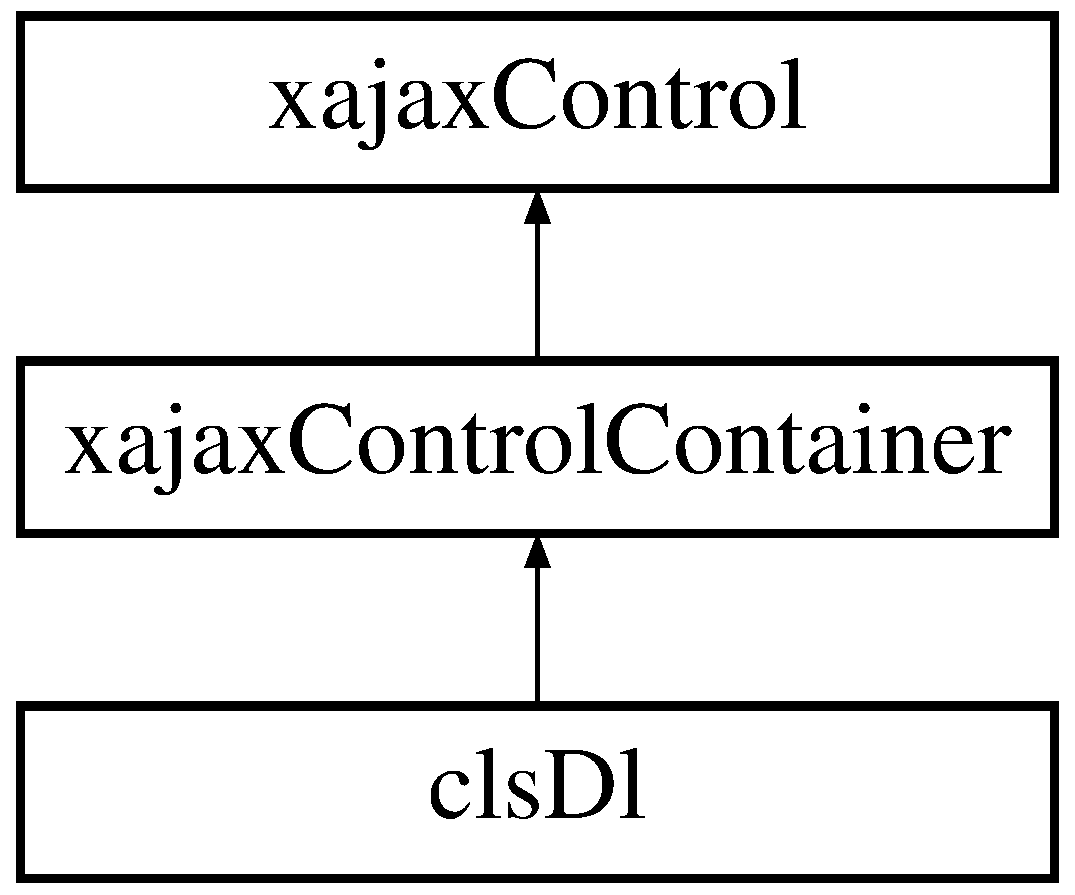
\includegraphics[height=3.000000cm]{classclsDl}
\end{center}
\end{figure}
\subsection*{Public Member Functions}
\begin{DoxyCompactItemize}
\item 
\hypertarget{classclsDl_a81e6adce5c22659e12c1ad7c8659b841}{
{\bfseries clsDl} (\$aConfiguration=array())}
\label{classclsDl_a81e6adce5c22659e12c1ad7c8659b841}

\end{DoxyCompactItemize}


\subsection{Detailed Description}


Definition at line 110 of file group.inc.php.



The documentation for this class was generated from the following file:\begin{DoxyCompactItemize}
\item 
xajax\_\-controls/group.inc.php\end{DoxyCompactItemize}

\hypertarget{classclsDoctype}{
\section{clsDoctype Class Reference}
\label{classclsDoctype}\index{clsDoctype@{clsDoctype}}
}
Inheritance diagram for clsDoctype:\begin{figure}[H]
\begin{center}
\leavevmode
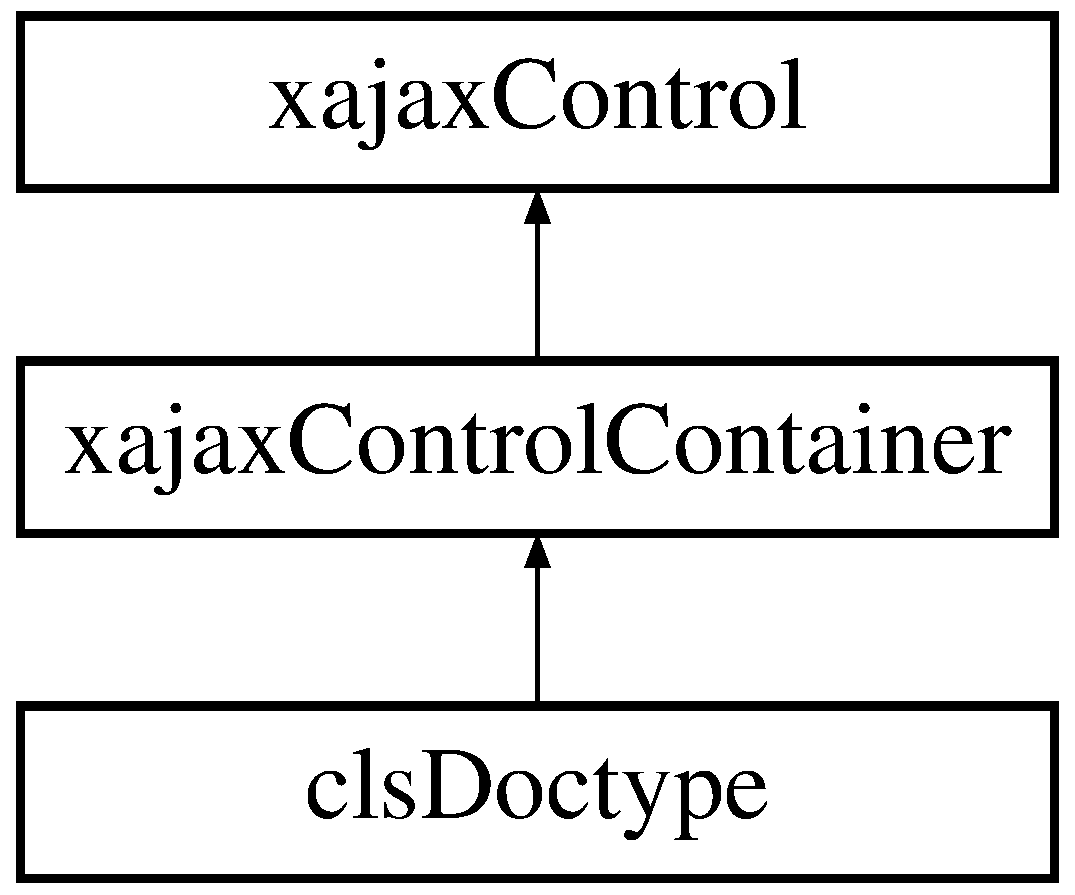
\includegraphics[height=3.000000cm]{classclsDoctype}
\end{center}
\end{figure}
\subsection*{Public Member Functions}
\begin{DoxyCompactItemize}
\item 
\hypertarget{classclsDoctype_a27e599976c2dda621846304a40b09f7f}{
{\bfseries clsDocType} (\$sFormat=null, \$sVersion=null, \$sValidation=null, \$sEncoding='UTF-\/8')}
\label{classclsDoctype_a27e599976c2dda621846304a40b09f7f}

\item 
\hypertarget{classclsDoctype_a0fcca7ea088614edd05d33c005ab3e89}{
{\bfseries printHTML} (\$sIndent='')}
\label{classclsDoctype_a0fcca7ea088614edd05d33c005ab3e89}

\end{DoxyCompactItemize}
\subsection*{Public Attributes}
\begin{DoxyCompactItemize}
\item 
\hypertarget{classclsDoctype_a47d587cd2523b4e4360f922be0f74a0d}{
{\bfseries \$sText}}
\label{classclsDoctype_a47d587cd2523b4e4360f922be0f74a0d}

\item 
\hypertarget{classclsDoctype_a80d1dff016b2d7ebd24fcc5803ab8090}{
{\bfseries \$sFormat}}
\label{classclsDoctype_a80d1dff016b2d7ebd24fcc5803ab8090}

\item 
\hypertarget{classclsDoctype_a6759e4615d4062ecbdeac76d0ff7032f}{
{\bfseries \$sVersion}}
\label{classclsDoctype_a6759e4615d4062ecbdeac76d0ff7032f}

\item 
\hypertarget{classclsDoctype_accc48bd77429ca2008389b3f12dec199}{
{\bfseries \$sValidation}}
\label{classclsDoctype_accc48bd77429ca2008389b3f12dec199}

\item 
\hypertarget{classclsDoctype_aaa9ecedebec197f86356f954e4331437}{
{\bfseries \$sEncoding}}
\label{classclsDoctype_aaa9ecedebec197f86356f954e4331437}

\end{DoxyCompactItemize}


\subsection{Detailed Description}


Definition at line 67 of file document.inc.php.



The documentation for this class was generated from the following file:\begin{DoxyCompactItemize}
\item 
xajax\_\-controls/document.inc.php\end{DoxyCompactItemize}

\hypertarget{classclsDocument}{
\section{clsDocument Class Reference}
\label{classclsDocument}\index{clsDocument@{clsDocument}}
}
Inheritance diagram for clsDocument:\begin{figure}[H]
\begin{center}
\leavevmode
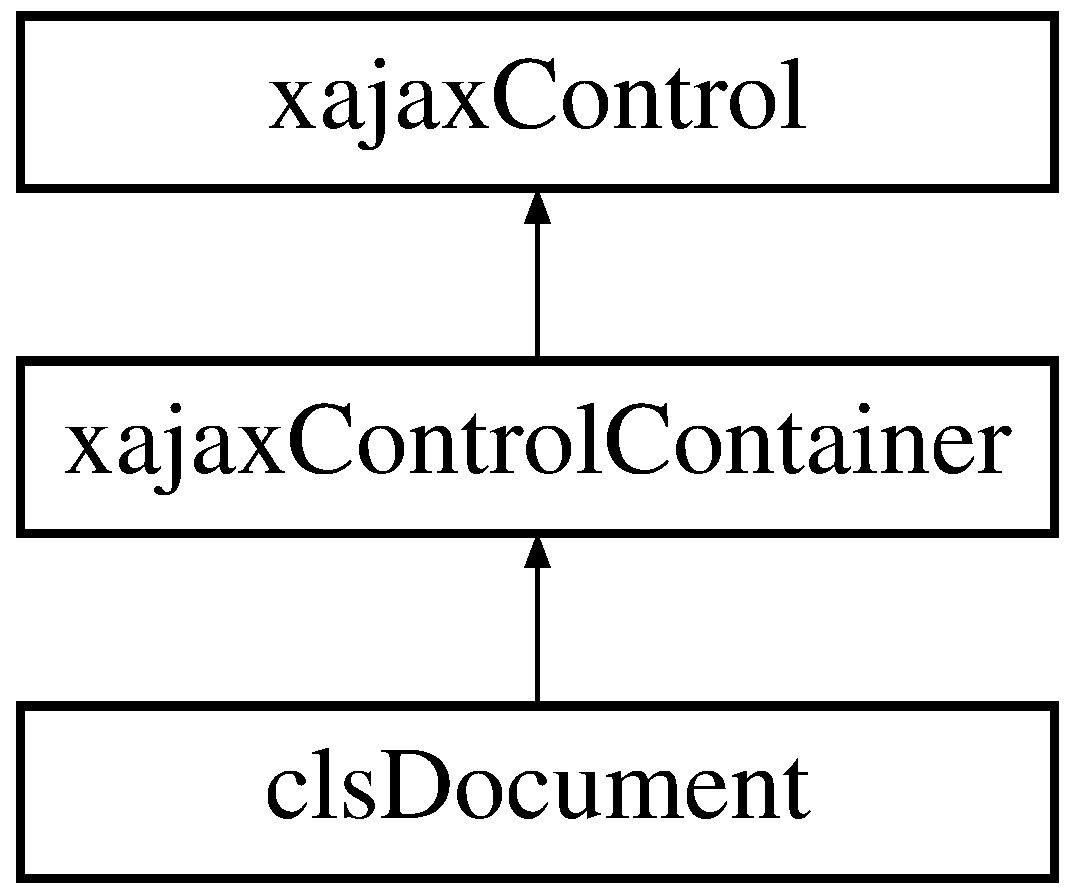
\includegraphics[height=3.000000cm]{classclsDocument}
\end{center}
\end{figure}
\subsection*{Public Member Functions}
\begin{DoxyCompactItemize}
\item 
\hypertarget{classclsDocument_a22b4994dc5739e02333c4974994b20a7}{
{\bfseries clsDocument} (\$aConfiguration=array())}
\label{classclsDocument_a22b4994dc5739e02333c4974994b20a7}

\item 
\hypertarget{classclsDocument_ad20d8a7c5539a351469ee98f98a88978}{
{\bfseries printHTML} ()}
\label{classclsDocument_ad20d8a7c5539a351469ee98f98a88978}

\end{DoxyCompactItemize}


\subsection{Detailed Description}


Definition at line 37 of file document.inc.php.



The documentation for this class was generated from the following file:\begin{DoxyCompactItemize}
\item 
xajax\_\-controls/document.inc.php\end{DoxyCompactItemize}

\hypertarget{classclsDt}{
\section{clsDt Class Reference}
\label{classclsDt}\index{clsDt@{clsDt}}
}
Inheritance diagram for clsDt:\begin{figure}[H]
\begin{center}
\leavevmode
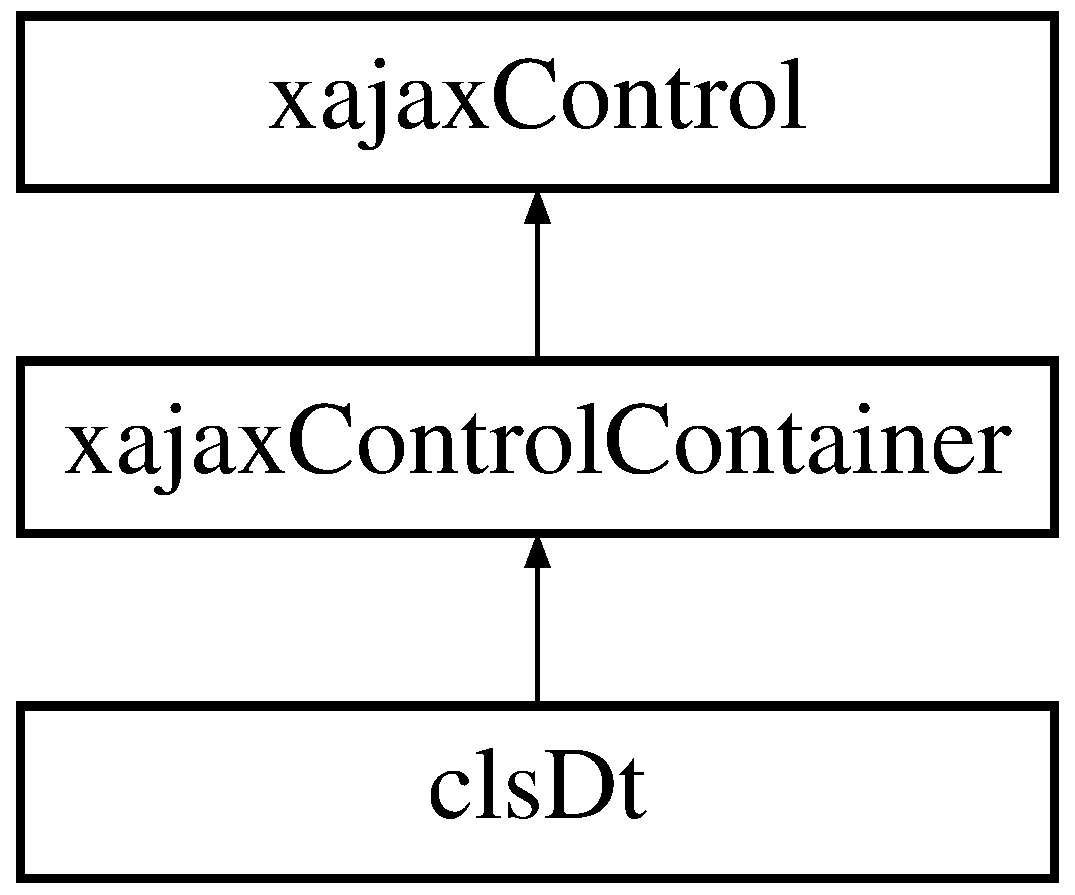
\includegraphics[height=3.000000cm]{classclsDt}
\end{center}
\end{figure}
\subsection*{Public Member Functions}
\begin{DoxyCompactItemize}
\item 
\hypertarget{classclsDt_a06eb7b38fa80f82fb8b7f4ea688edf05}{
{\bfseries clsDt} (\$aConfiguration=array())}
\label{classclsDt_a06eb7b38fa80f82fb8b7f4ea688edf05}

\end{DoxyCompactItemize}


\subsection{Detailed Description}


Definition at line 120 of file group.inc.php.



The documentation for this class was generated from the following file:\begin{DoxyCompactItemize}
\item 
xajax\_\-controls/group.inc.php\end{DoxyCompactItemize}

\hypertarget{classclsEm}{
\section{clsEm Class Reference}
\label{classclsEm}\index{clsEm@{clsEm}}
}
Inheritance diagram for clsEm:\begin{figure}[H]
\begin{center}
\leavevmode
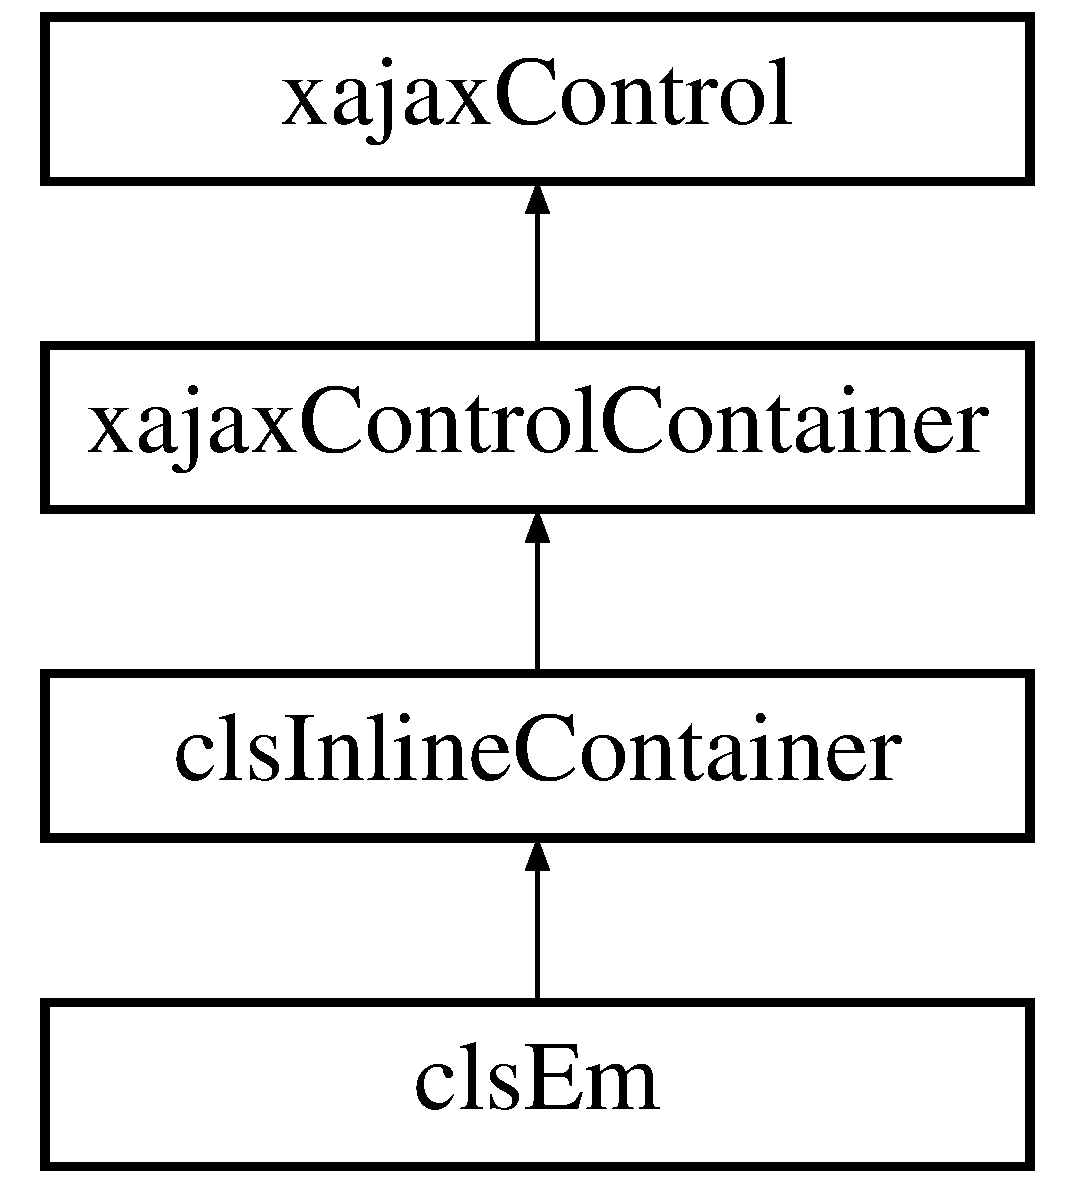
\includegraphics[height=4.000000cm]{classclsEm}
\end{center}
\end{figure}
\subsection*{Public Member Functions}
\begin{DoxyCompactItemize}
\item 
\hypertarget{classclsEm_abf003a775bb7cf01a6b2fbb480e5291f}{
{\bfseries clsEm} (\$aConfiguration=array())}
\label{classclsEm_abf003a775bb7cf01a6b2fbb480e5291f}

\end{DoxyCompactItemize}


\subsection{Detailed Description}


Definition at line 101 of file content.inc.php.



The documentation for this class was generated from the following file:\begin{DoxyCompactItemize}
\item 
xajax\_\-controls/content.inc.php\end{DoxyCompactItemize}

\hypertarget{classclsEventHandlers}{
\section{clsEventHandlers Class Reference}
\label{classclsEventHandlers}\index{clsEventHandlers@{clsEventHandlers}}
}
\subsection*{Public Member Functions}
\begin{DoxyCompactItemize}
\item 
\hypertarget{classclsEventHandlers_ad7c1bfbc772d852356aa0ec244a88254}{
{\bfseries eventHandlerThree} ()}
\label{classclsEventHandlers_ad7c1bfbc772d852356aa0ec244a88254}

\end{DoxyCompactItemize}


\subsection{Detailed Description}


Definition at line 26 of file server\_\-events.php.



The documentation for this class was generated from the following file:\begin{DoxyCompactItemize}
\item 
tests/suite/server\_\-events.php\end{DoxyCompactItemize}

\hypertarget{classclsFieldset}{
\section{clsFieldset Class Reference}
\label{classclsFieldset}\index{clsFieldset@{clsFieldset}}
}
Inheritance diagram for clsFieldset:\begin{figure}[H]
\begin{center}
\leavevmode
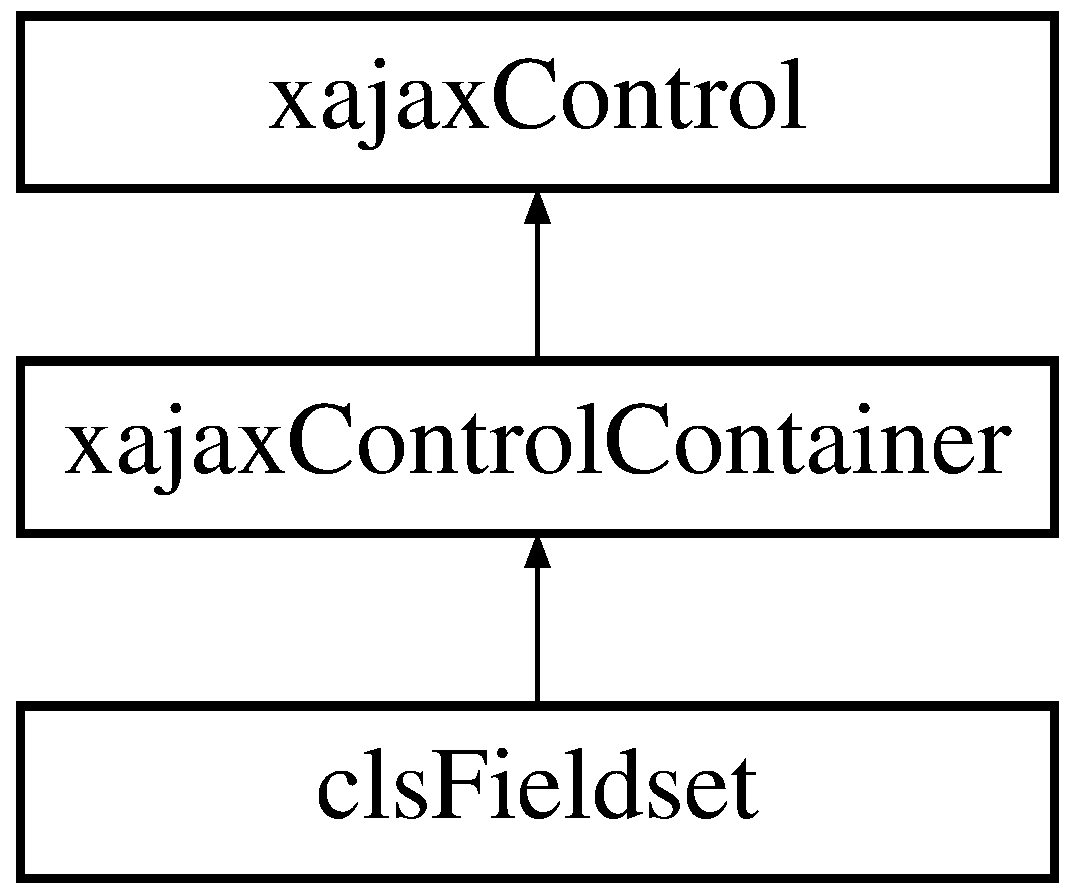
\includegraphics[height=3.000000cm]{classclsFieldset}
\end{center}
\end{figure}
\subsection*{Public Member Functions}
\begin{DoxyCompactItemize}
\item 
\hypertarget{classclsFieldset_a0ac441594dd63874416d1fc87fd37f8d}{
{\bfseries clsFieldset} (\$aConfiguration=array())}
\label{classclsFieldset_a0ac441594dd63874416d1fc87fd37f8d}

\end{DoxyCompactItemize}


\subsection{Detailed Description}


Definition at line 297 of file form.inc.php.



The documentation for this class was generated from the following file:\begin{DoxyCompactItemize}
\item 
xajax\_\-controls/form.inc.php\end{DoxyCompactItemize}

\hypertarget{classclsForm}{
\section{clsForm Class Reference}
\label{classclsForm}\index{clsForm@{clsForm}}
}
Inheritance diagram for clsForm:\begin{figure}[H]
\begin{center}
\leavevmode
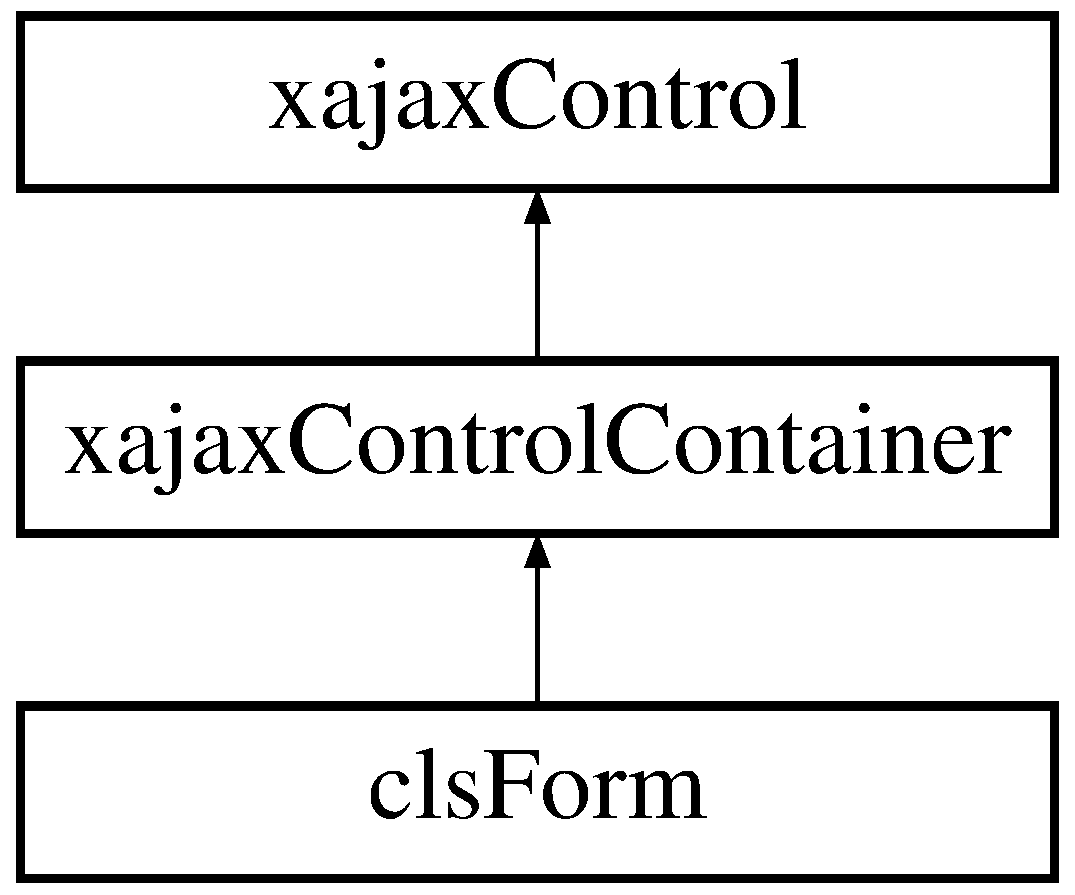
\includegraphics[height=3.000000cm]{classclsForm}
\end{center}
\end{figure}
\subsection*{Public Member Functions}
\begin{DoxyCompactItemize}
\item 
\hypertarget{classclsForm_a6f0fdbc3f48b17243405de32671da96d}{
{\bfseries clsForm} (\$aConfiguration=array())}
\label{classclsForm_a6f0fdbc3f48b17243405de32671da96d}

\end{DoxyCompactItemize}


\subsection{Detailed Description}


Definition at line 37 of file form.inc.php.



The documentation for this class was generated from the following file:\begin{DoxyCompactItemize}
\item 
xajax\_\-controls/form.inc.php\end{DoxyCompactItemize}

\hypertarget{classclsFrame}{
\section{clsFrame Class Reference}
\label{classclsFrame}\index{clsFrame@{clsFrame}}
}
Inheritance diagram for clsFrame:\begin{figure}[H]
\begin{center}
\leavevmode
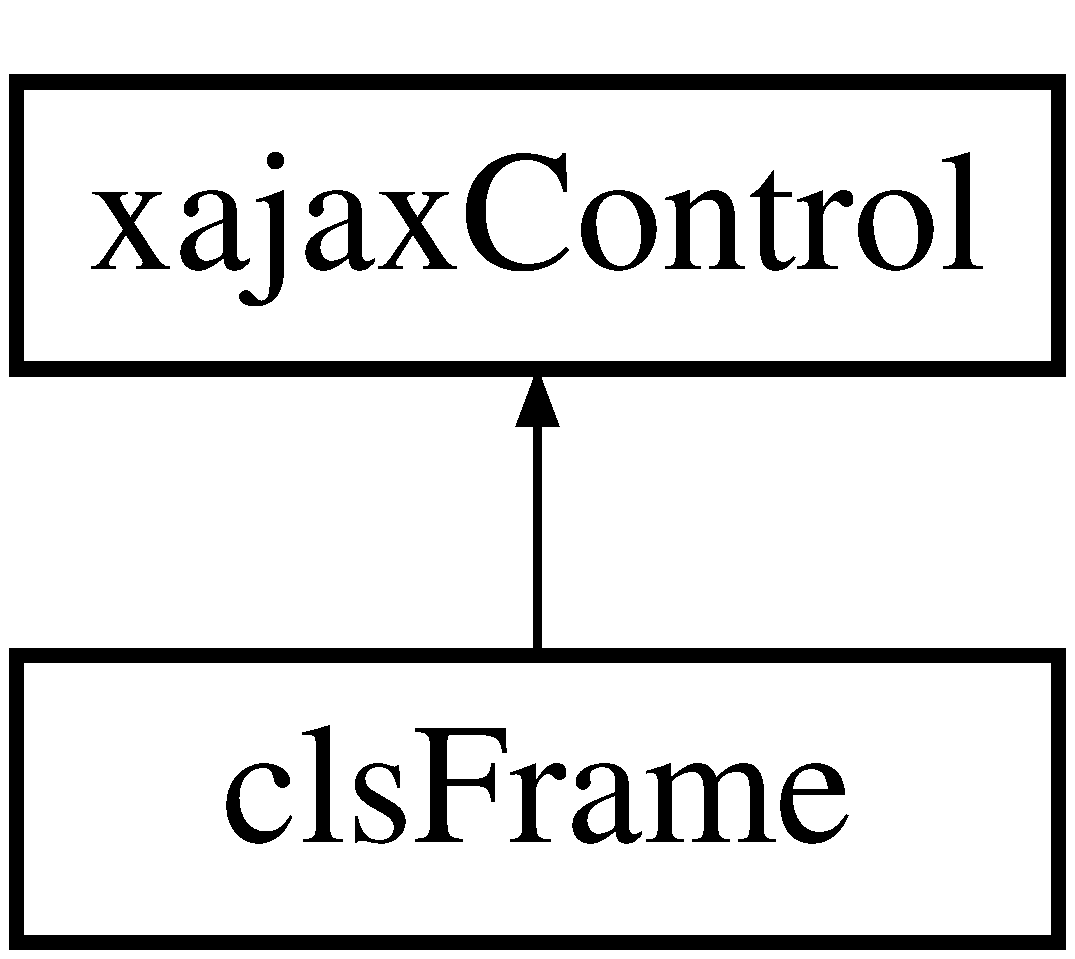
\includegraphics[height=2.000000cm]{classclsFrame}
\end{center}
\end{figure}
\subsection*{Public Member Functions}
\begin{DoxyCompactItemize}
\item 
\hypertarget{classclsFrame_aa63d9453d7cd8a8fd4bf9d5da33affe9}{
{\bfseries clsFrame} (\$aConfiguration=array())}
\label{classclsFrame_aa63d9453d7cd8a8fd4bf9d5da33affe9}

\end{DoxyCompactItemize}


\subsection{Detailed Description}


Definition at line 306 of file document.inc.php.



The documentation for this class was generated from the following file:\begin{DoxyCompactItemize}
\item 
xajax\_\-controls/document.inc.php\end{DoxyCompactItemize}

\hypertarget{classclsFrameset}{
\section{clsFrameset Class Reference}
\label{classclsFrameset}\index{clsFrameset@{clsFrameset}}
}
Inheritance diagram for clsFrameset:\begin{figure}[H]
\begin{center}
\leavevmode
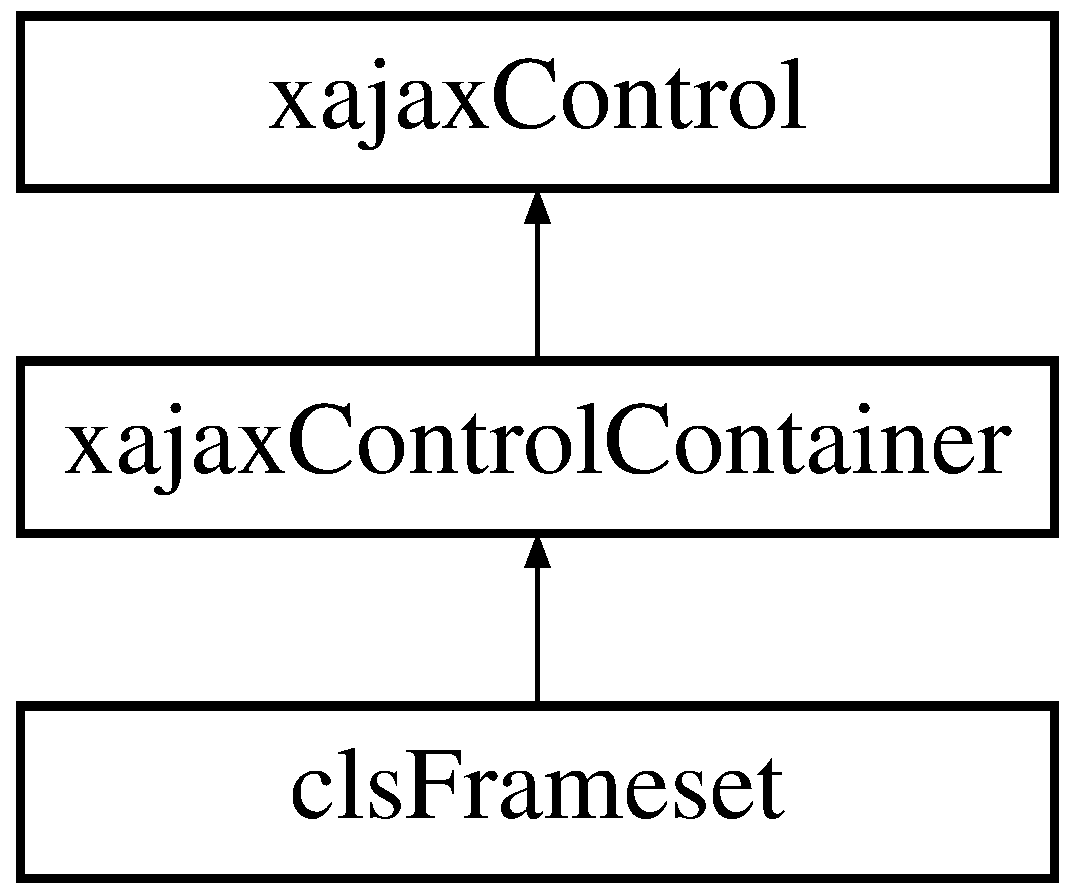
\includegraphics[height=3.000000cm]{classclsFrameset}
\end{center}
\end{figure}
\subsection*{Public Member Functions}
\begin{DoxyCompactItemize}
\item 
\hypertarget{classclsFrameset_adaa8009a91ac52797f4b9d7e697e3d0e}{
{\bfseries clsFrameset} (\$aConfiguration=array())}
\label{classclsFrameset_adaa8009a91ac52797f4b9d7e697e3d0e}

\end{DoxyCompactItemize}


\subsection{Detailed Description}


Definition at line 296 of file document.inc.php.



The documentation for this class was generated from the following file:\begin{DoxyCompactItemize}
\item 
xajax\_\-controls/document.inc.php\end{DoxyCompactItemize}

\hypertarget{classclsFunctions}{
\section{clsFunctions Class Reference}
\label{classclsFunctions}\index{clsFunctions@{clsFunctions}}
}
\subsection*{Public Member Functions}
\begin{DoxyCompactItemize}
\item 
\hypertarget{classclsFunctions_ae44809d49334b5c385b7fd4b1e0d195c}{
{\bfseries clsFunctions} ()}
\label{classclsFunctions_ae44809d49334b5c385b7fd4b1e0d195c}

\item 
\hypertarget{classclsFunctions_a6af9864b8cf3b37222c35fc0ab096169}{
{\bfseries loadCSS1} ()}
\label{classclsFunctions_a6af9864b8cf3b37222c35fc0ab096169}

\item 
\hypertarget{classclsFunctions_a67814b64ee7a66cc8271a0edf91c5579}{
{\bfseries unloadCSS1} ()}
\label{classclsFunctions_a67814b64ee7a66cc8271a0edf91c5579}

\item 
\hypertarget{classclsFunctions_a074a5bb992e077d623e2a096b593f873}{
{\bfseries loadCSS2} ()}
\label{classclsFunctions_a074a5bb992e077d623e2a096b593f873}

\item 
\hypertarget{classclsFunctions_a9f05c710fa25a33d7fd91757262c1d1e}{
{\bfseries unloadCSS2} ()}
\label{classclsFunctions_a9f05c710fa25a33d7fd91757262c1d1e}

\item 
\hypertarget{classclsFunctions_ad8f9ff0cfbb23c99c2925c9a7a1e2b25}{
{\bfseries loadCSS1\_\-Print} ()}
\label{classclsFunctions_ad8f9ff0cfbb23c99c2925c9a7a1e2b25}

\item 
\hypertarget{classclsFunctions_ae01c2807f5c7a0548f111ca2c15919c7}{
{\bfseries unloadCSS1\_\-Print} ()}
\label{classclsFunctions_ae01c2807f5c7a0548f111ca2c15919c7}

\item 
\hypertarget{classclsFunctions_affd6ae2d0332ea9332c397657ec32d8f}{
{\bfseries loadCSS2\_\-Print} ()}
\label{classclsFunctions_affd6ae2d0332ea9332c397657ec32d8f}

\item 
\hypertarget{classclsFunctions_a5d66e381f933e6c882fe7b23e2f71654}{
{\bfseries unloadCSS2\_\-Print} ()}
\label{classclsFunctions_a5d66e381f933e6c882fe7b23e2f71654}

\item 
\hypertarget{classclsFunctions_ae44809d49334b5c385b7fd4b1e0d195c}{
{\bfseries clsFunctions} ()}
\label{classclsFunctions_ae44809d49334b5c385b7fd4b1e0d195c}

\item 
\hypertarget{classclsFunctions_a0bd6dd64bf2bcdf6cba5d3de8edd5f02}{
{\bfseries showIsLoaded} ()}
\label{classclsFunctions_a0bd6dd64bf2bcdf6cba5d3de8edd5f02}

\item 
\hypertarget{classclsFunctions_a6be142ebcc35e929ecac5dbf84db4863}{
{\bfseries showFormValues} (\$aFormValues)}
\label{classclsFunctions_a6be142ebcc35e929ecac5dbf84db4863}

\item 
\hypertarget{classclsFunctions_af56ddbe38a38dc9dcf88bdd3b0a89887}{
{\bfseries clear} ()}
\label{classclsFunctions_af56ddbe38a38dc9dcf88bdd3b0a89887}

\item 
\hypertarget{classclsFunctions_ae44809d49334b5c385b7fd4b1e0d195c}{
{\bfseries clsFunctions} ()}
\label{classclsFunctions_ae44809d49334b5c385b7fd4b1e0d195c}

\item 
\hypertarget{classclsFunctions_a225ea1cc121fb89698bc2839ae8decc6}{
{\bfseries confirm} (\$seconds)}
\label{classclsFunctions_a225ea1cc121fb89698bc2839ae8decc6}

\end{DoxyCompactItemize}


\subsection{Detailed Description}


Definition at line 17 of file css.php.



The documentation for this class was generated from the following files:\begin{DoxyCompactItemize}
\item 
tests/suite/css.php\item 
tests/suite/iframe.php\item 
tests/suite/theFrame.php\end{DoxyCompactItemize}

\hypertarget{classclsGoogleMap}{
\section{clsGoogleMap Class Reference}
\label{classclsGoogleMap}\index{clsGoogleMap@{clsGoogleMap}}
}
Inheritance diagram for clsGoogleMap:\begin{figure}[H]
\begin{center}
\leavevmode
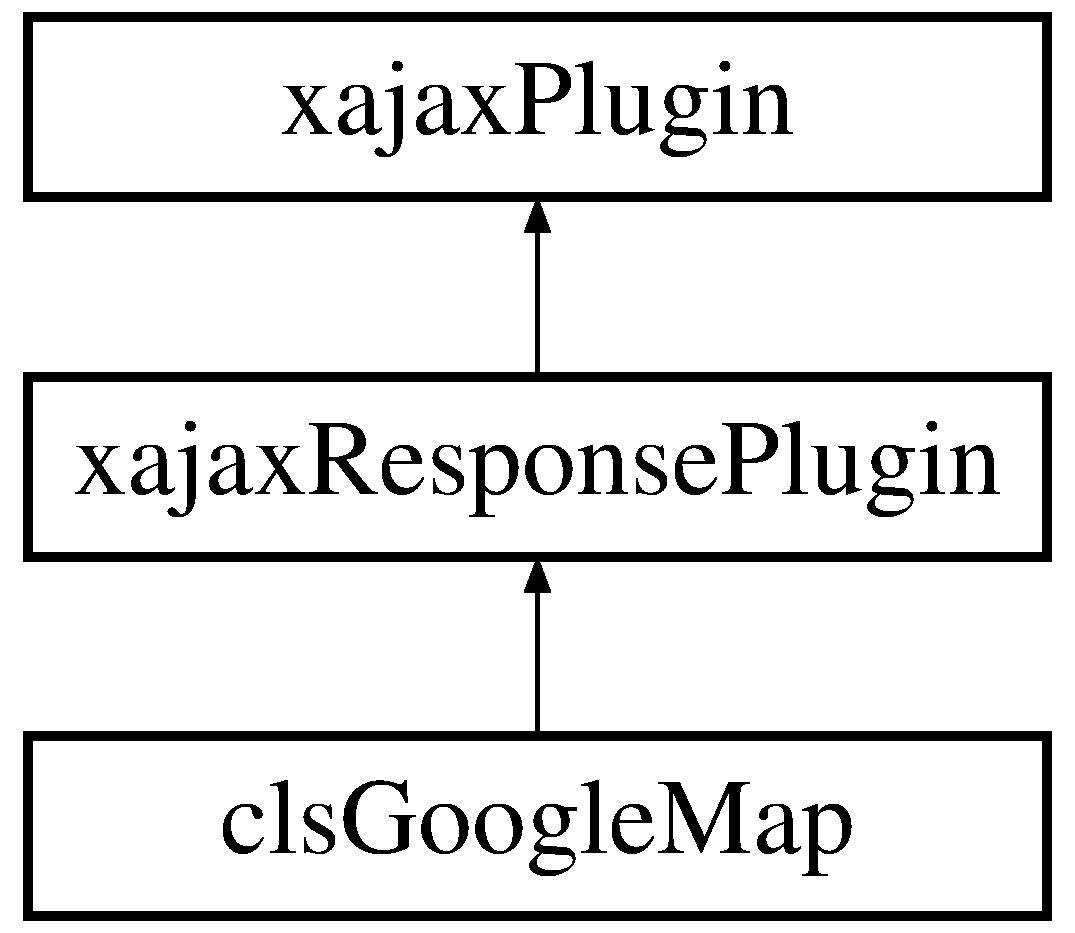
\includegraphics[height=3.000000cm]{classclsGoogleMap}
\end{center}
\end{figure}
\subsection*{Public Member Functions}
\begin{DoxyCompactItemize}
\item 
\hypertarget{classclsGoogleMap_a03f1e7a6a2916de95bda07dab3bc4f23}{
{\bfseries clsGoogleMap} ()}
\label{classclsGoogleMap_a03f1e7a6a2916de95bda07dab3bc4f23}

\item 
\hypertarget{classclsGoogleMap_a3eb5df55b60014f3596ff2257a4e113a}{
{\bfseries configure} (\$sName, \$mValue)}
\label{classclsGoogleMap_a3eb5df55b60014f3596ff2257a4e113a}

\item 
\hypertarget{classclsGoogleMap_a56701d2d8c9222b23e10265ef591cb2f}{
{\bfseries generateClientScript} ()}
\label{classclsGoogleMap_a56701d2d8c9222b23e10265ef591cb2f}

\item 
\hypertarget{classclsGoogleMap_ac0fa04ea8344038f8bfa9c2248533989}{
{\bfseries getName} ()}
\label{classclsGoogleMap_ac0fa04ea8344038f8bfa9c2248533989}

\item 
\hypertarget{classclsGoogleMap_ad474087da1030f8b51567de73affe482}{
{\bfseries setGoogleSiteKey} (\$sKey)}
\label{classclsGoogleMap_ad474087da1030f8b51567de73affe482}

\item 
\hypertarget{classclsGoogleMap_a08b6376d826504bd1f390ffb725dfabb}{
{\bfseries create} (\$sMap, \$sParentId)}
\label{classclsGoogleMap_a08b6376d826504bd1f390ffb725dfabb}

\item 
\hypertarget{classclsGoogleMap_adf07b37e7e297651b206461039c180ae}{
{\bfseries zoom} (\$sMap, \$nZoom)}
\label{classclsGoogleMap_adf07b37e7e297651b206461039c180ae}

\item 
\hypertarget{classclsGoogleMap_a097b0acbe6487b9fc6631146b859061c}{
{\bfseries setMarker} (\$sMap, \$nLat, \$nLon, \$sText)}
\label{classclsGoogleMap_a097b0acbe6487b9fc6631146b859061c}

\item 
\hypertarget{classclsGoogleMap_a5477c2c0f0ca6a6df19ee35449d76230}{
{\bfseries moveTo} (\$sMap, \$nLat, \$nLon)}
\label{classclsGoogleMap_a5477c2c0f0ca6a6df19ee35449d76230}

\end{DoxyCompactItemize}
\subsection*{Public Attributes}
\begin{DoxyCompactItemize}
\item 
\hypertarget{classclsGoogleMap_a6dfcdb1b7ab776d43d048633107fe7a1}{
{\bfseries \$sJavascriptURI}}
\label{classclsGoogleMap_a6dfcdb1b7ab776d43d048633107fe7a1}

\item 
\hypertarget{classclsGoogleMap_a80916c730906f660153bdb3d0aed8fc3}{
{\bfseries \$bInlineScript}}
\label{classclsGoogleMap_a80916c730906f660153bdb3d0aed8fc3}

\end{DoxyCompactItemize}


\subsection{Detailed Description}


Definition at line 23 of file googleMap.inc.php.



The documentation for this class was generated from the following file:\begin{DoxyCompactItemize}
\item 
xajax\_\-plugins/response/googleMap.inc.php\end{DoxyCompactItemize}

\hypertarget{classclsHead}{
\section{clsHead Class Reference}
\label{classclsHead}\index{clsHead@{clsHead}}
}
Inheritance diagram for clsHead:\begin{figure}[H]
\begin{center}
\leavevmode
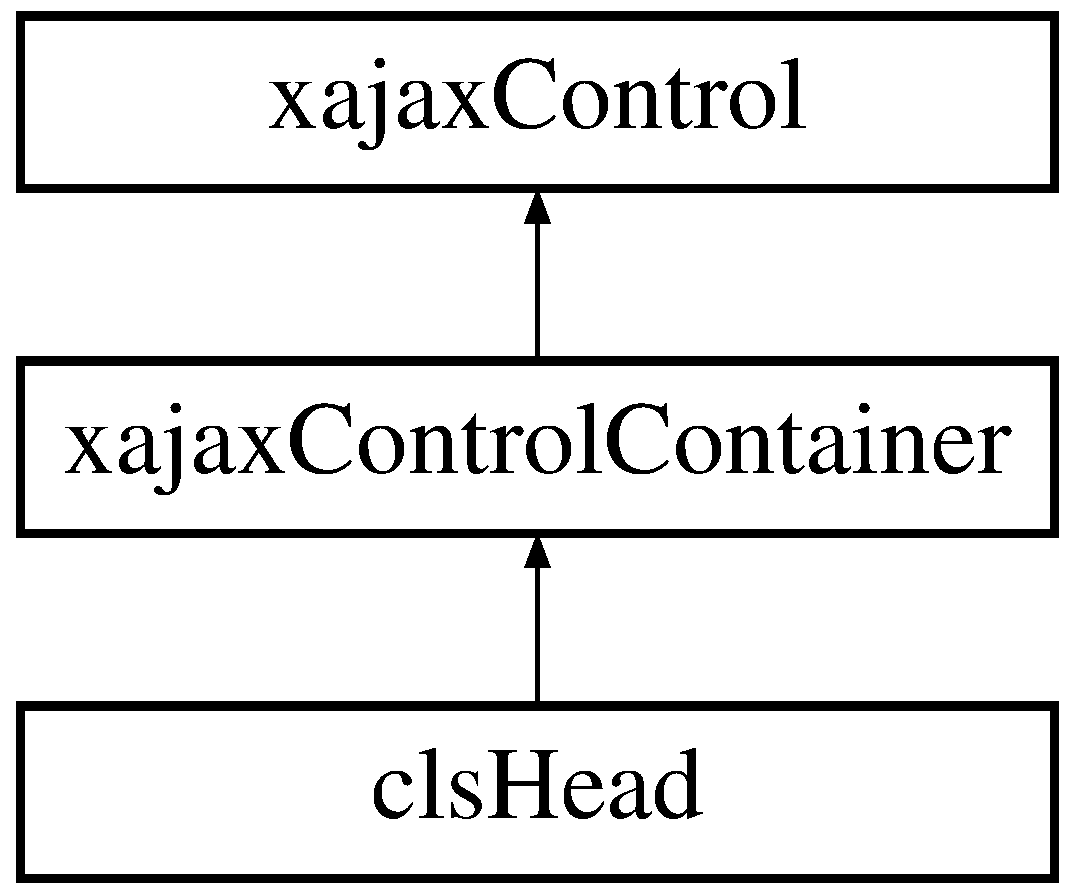
\includegraphics[height=3.000000cm]{classclsHead}
\end{center}
\end{figure}
\subsection*{Public Member Functions}
\begin{DoxyCompactItemize}
\item 
\hypertarget{classclsHead_a3b45efa7b4d4dd5f23b3ecaf8374e1f7}{
{\bfseries clsHead} (\$aConfiguration=array())}
\label{classclsHead_a3b45efa7b4d4dd5f23b3ecaf8374e1f7}

\item 
\hypertarget{classclsHead_ab5b43e8666645ab386e2f968c6f4cc74}{
{\bfseries setXajax} (\&\$objXajax)}
\label{classclsHead_ab5b43e8666645ab386e2f968c6f4cc74}

\item 
\hypertarget{classclsHead_a902dddda68fd8274f4a0b0c5980c6e55}{
{\bfseries \_\-printChildren} (\$sIndent='')}
\label{classclsHead_a902dddda68fd8274f4a0b0c5980c6e55}

\end{DoxyCompactItemize}
\subsection*{Public Attributes}
\begin{DoxyCompactItemize}
\item 
\hypertarget{classclsHead_a6c24c6adc16c9daf5148b7691b817b4b}{
{\bfseries \$objXajax}}
\label{classclsHead_a6c24c6adc16c9daf5148b7691b817b4b}

\end{DoxyCompactItemize}


\subsection{Detailed Description}


Definition at line 167 of file document.inc.php.



The documentation for this class was generated from the following file:\begin{DoxyCompactItemize}
\item 
xajax\_\-controls/document.inc.php\end{DoxyCompactItemize}

\hypertarget{classclsHeadline}{
\section{clsHeadline Class Reference}
\label{classclsHeadline}\index{clsHeadline@{clsHeadline}}
}
Inheritance diagram for clsHeadline:\begin{figure}[H]
\begin{center}
\leavevmode
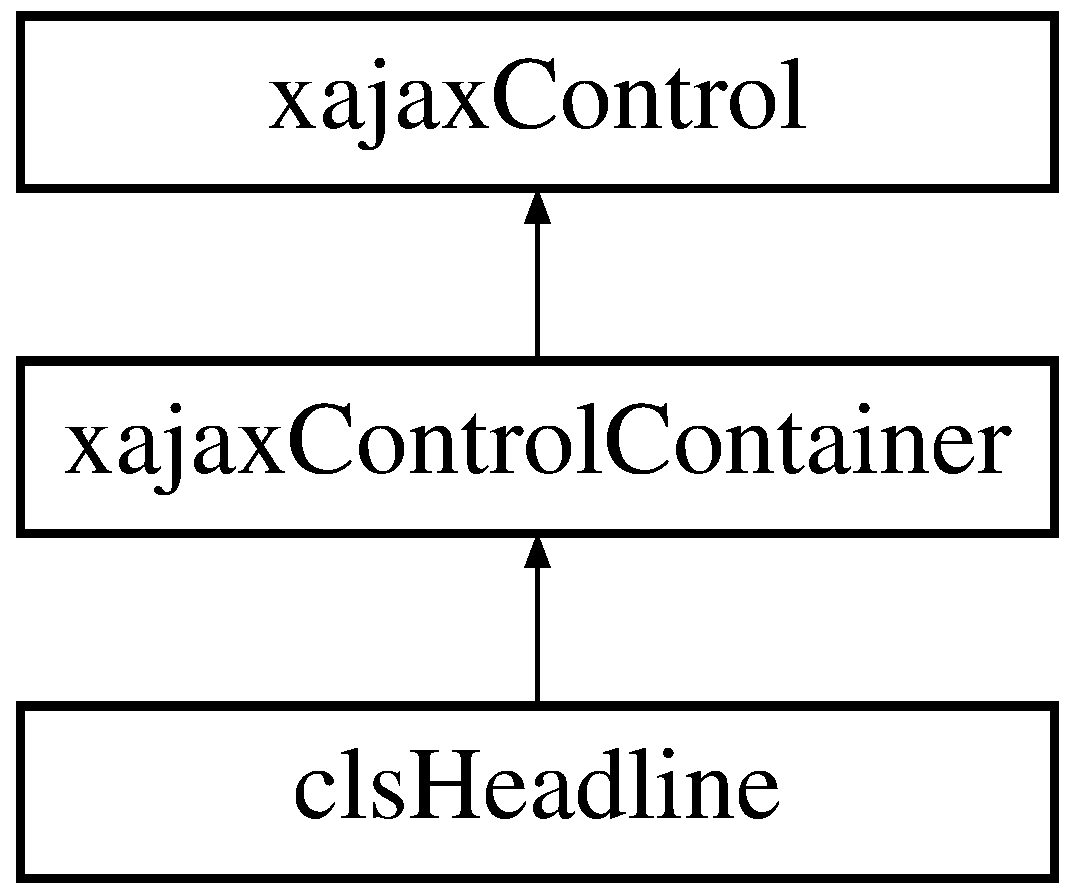
\includegraphics[height=3.000000cm]{classclsHeadline}
\end{center}
\end{figure}
\subsection*{Public Member Functions}
\begin{DoxyCompactItemize}
\item 
\hypertarget{classclsHeadline_af429d959224b68536104797350496c84}{
{\bfseries clsHeadline} (\$sType, \$aConfiguration=array())}
\label{classclsHeadline_af429d959224b68536104797350496c84}

\end{DoxyCompactItemize}


\subsection{Detailed Description}


Definition at line 238 of file content.inc.php.



The documentation for this class was generated from the following file:\begin{DoxyCompactItemize}
\item 
xajax\_\-controls/content.inc.php\end{DoxyCompactItemize}

\hypertarget{classclsHr}{
\section{clsHr Class Reference}
\label{classclsHr}\index{clsHr@{clsHr}}
}
Inheritance diagram for clsHr:\begin{figure}[H]
\begin{center}
\leavevmode
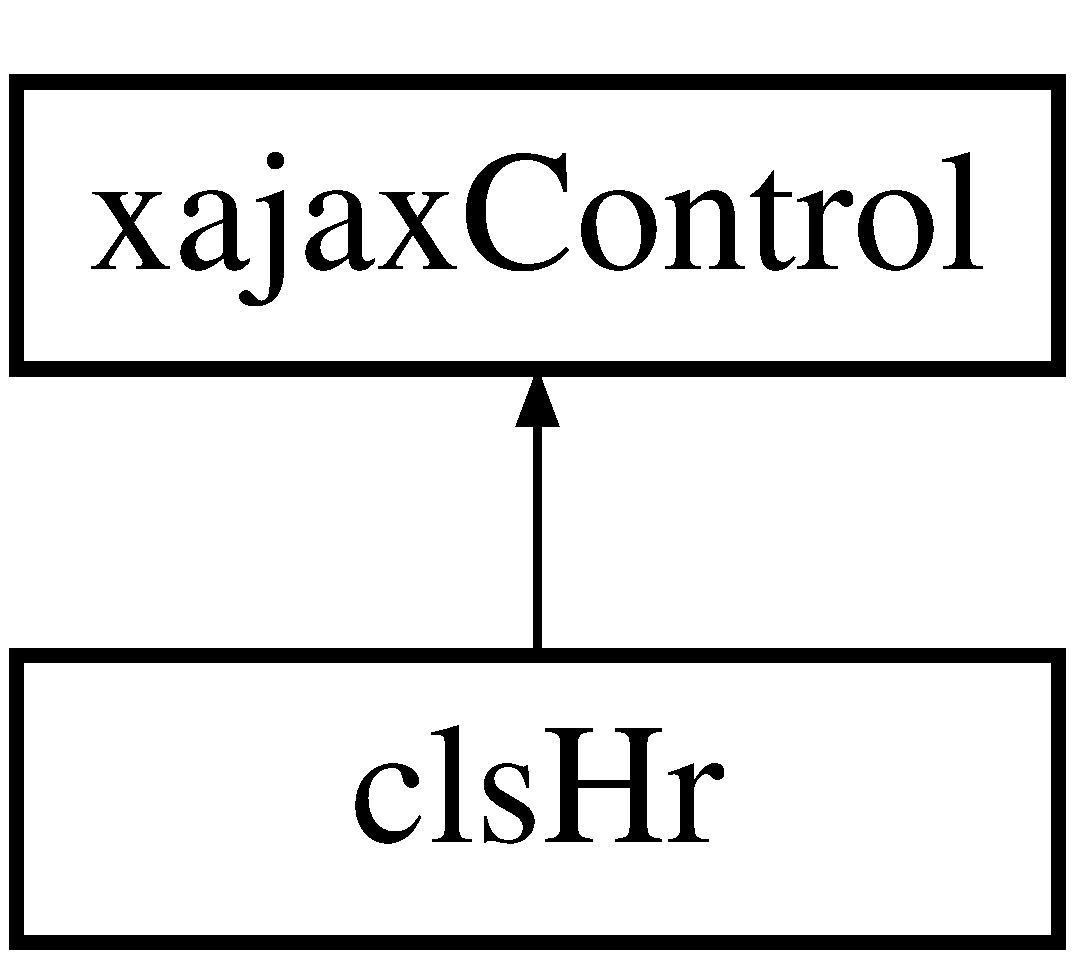
\includegraphics[height=2.000000cm]{classclsHr}
\end{center}
\end{figure}
\subsection*{Public Member Functions}
\begin{DoxyCompactItemize}
\item 
\hypertarget{classclsHr_a5e93df21b5a4663017a8d4bb4c9d3972}{
{\bfseries clsHr} (\$aConfiguration=array())}
\label{classclsHr_a5e93df21b5a4663017a8d4bb4c9d3972}

\end{DoxyCompactItemize}


\subsection{Detailed Description}


Definition at line 63 of file content.inc.php.



The documentation for this class was generated from the following file:\begin{DoxyCompactItemize}
\item 
xajax\_\-controls/content.inc.php\end{DoxyCompactItemize}

\hypertarget{classclsHtml}{
\section{clsHtml Class Reference}
\label{classclsHtml}\index{clsHtml@{clsHtml}}
}
Inheritance diagram for clsHtml:\begin{figure}[H]
\begin{center}
\leavevmode
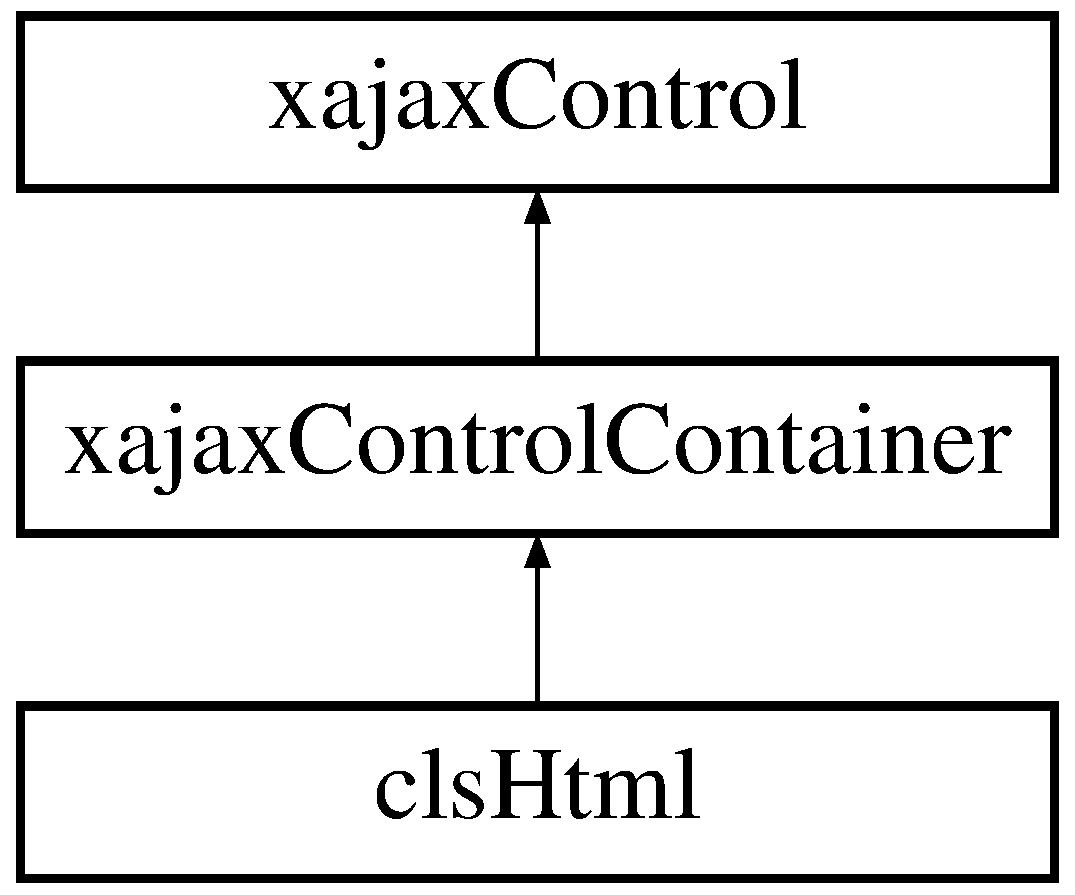
\includegraphics[height=3.000000cm]{classclsHtml}
\end{center}
\end{figure}
\subsection*{Public Member Functions}
\begin{DoxyCompactItemize}
\item 
\hypertarget{classclsHtml_a6bc277465cfaa9bc8086101bcd41780d}{
{\bfseries clsHtml} (\$aConfiguration=array())}
\label{classclsHtml_a6bc277465cfaa9bc8086101bcd41780d}

\end{DoxyCompactItemize}


\subsection{Detailed Description}


Definition at line 156 of file document.inc.php.



The documentation for this class was generated from the following file:\begin{DoxyCompactItemize}
\item 
xajax\_\-controls/document.inc.php\end{DoxyCompactItemize}

\hypertarget{classclsIframe}{
\section{clsIframe Class Reference}
\label{classclsIframe}\index{clsIframe@{clsIframe}}
}
Inheritance diagram for clsIframe:\begin{figure}[H]
\begin{center}
\leavevmode
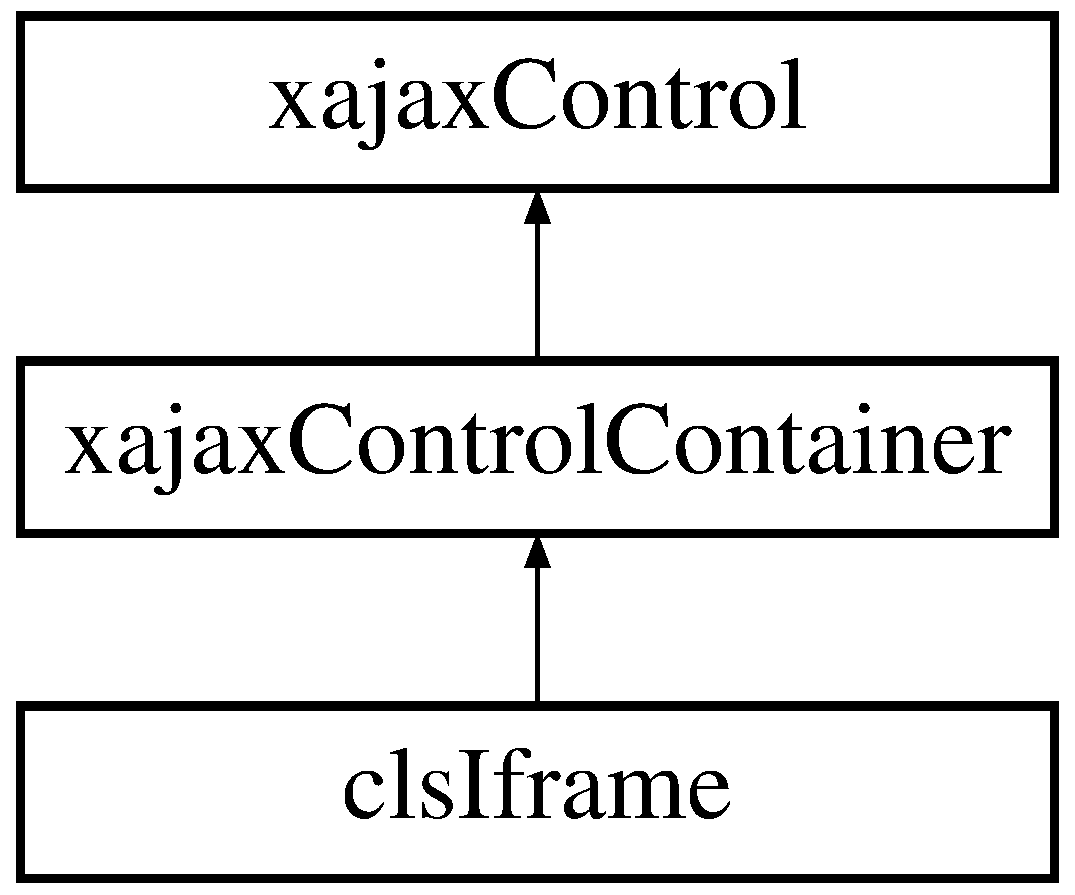
\includegraphics[height=3.000000cm]{classclsIframe}
\end{center}
\end{figure}
\subsection*{Public Member Functions}
\begin{DoxyCompactItemize}
\item 
\hypertarget{classclsIframe_a69c18cef43ce251dd8f96f80d44a96b5}{
{\bfseries clsIframe} (\$aConfiguration=array())}
\label{classclsIframe_a69c18cef43ce251dd8f96f80d44a96b5}

\end{DoxyCompactItemize}


\subsection{Detailed Description}


Definition at line 286 of file document.inc.php.



The documentation for this class was generated from the following file:\begin{DoxyCompactItemize}
\item 
xajax\_\-controls/document.inc.php\end{DoxyCompactItemize}

\hypertarget{classclsImg}{
\section{clsImg Class Reference}
\label{classclsImg}\index{clsImg@{clsImg}}
}
Inheritance diagram for clsImg:\begin{figure}[H]
\begin{center}
\leavevmode
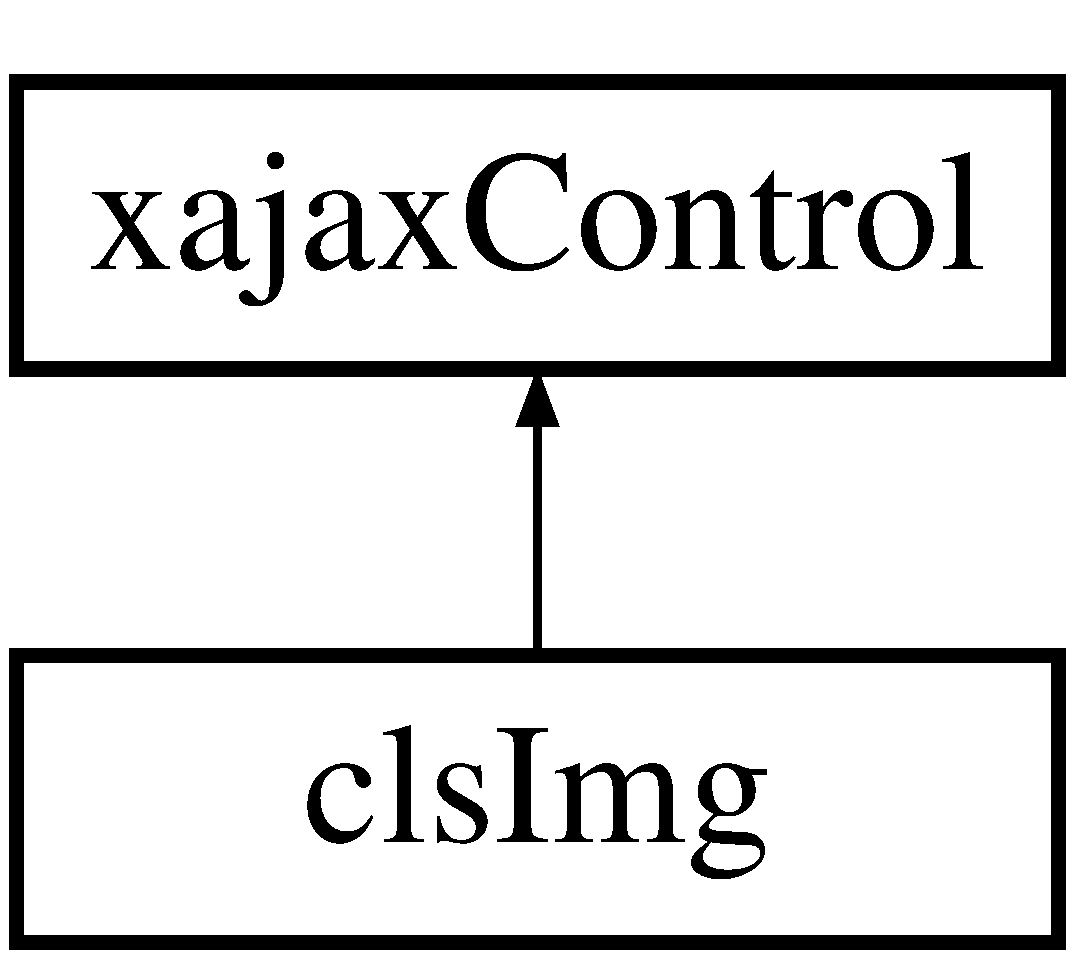
\includegraphics[height=2.000000cm]{classclsImg}
\end{center}
\end{figure}
\subsection*{Public Member Functions}
\begin{DoxyCompactItemize}
\item 
\hypertarget{classclsImg_aa6f61765d5effce995b6310fe226b037}{
{\bfseries clsImg} (\$aConfiguration=array())}
\label{classclsImg_aa6f61765d5effce995b6310fe226b037}

\end{DoxyCompactItemize}


\subsection{Detailed Description}


Definition at line 80 of file misc.inc.php.



The documentation for this class was generated from the following file:\begin{DoxyCompactItemize}
\item 
xajax\_\-controls/misc.inc.php\end{DoxyCompactItemize}

\hypertarget{classclsInlineContainer}{
\section{clsInlineContainer Class Reference}
\label{classclsInlineContainer}\index{clsInlineContainer@{clsInlineContainer}}
}
Inheritance diagram for clsInlineContainer:\begin{figure}[H]
\begin{center}
\leavevmode
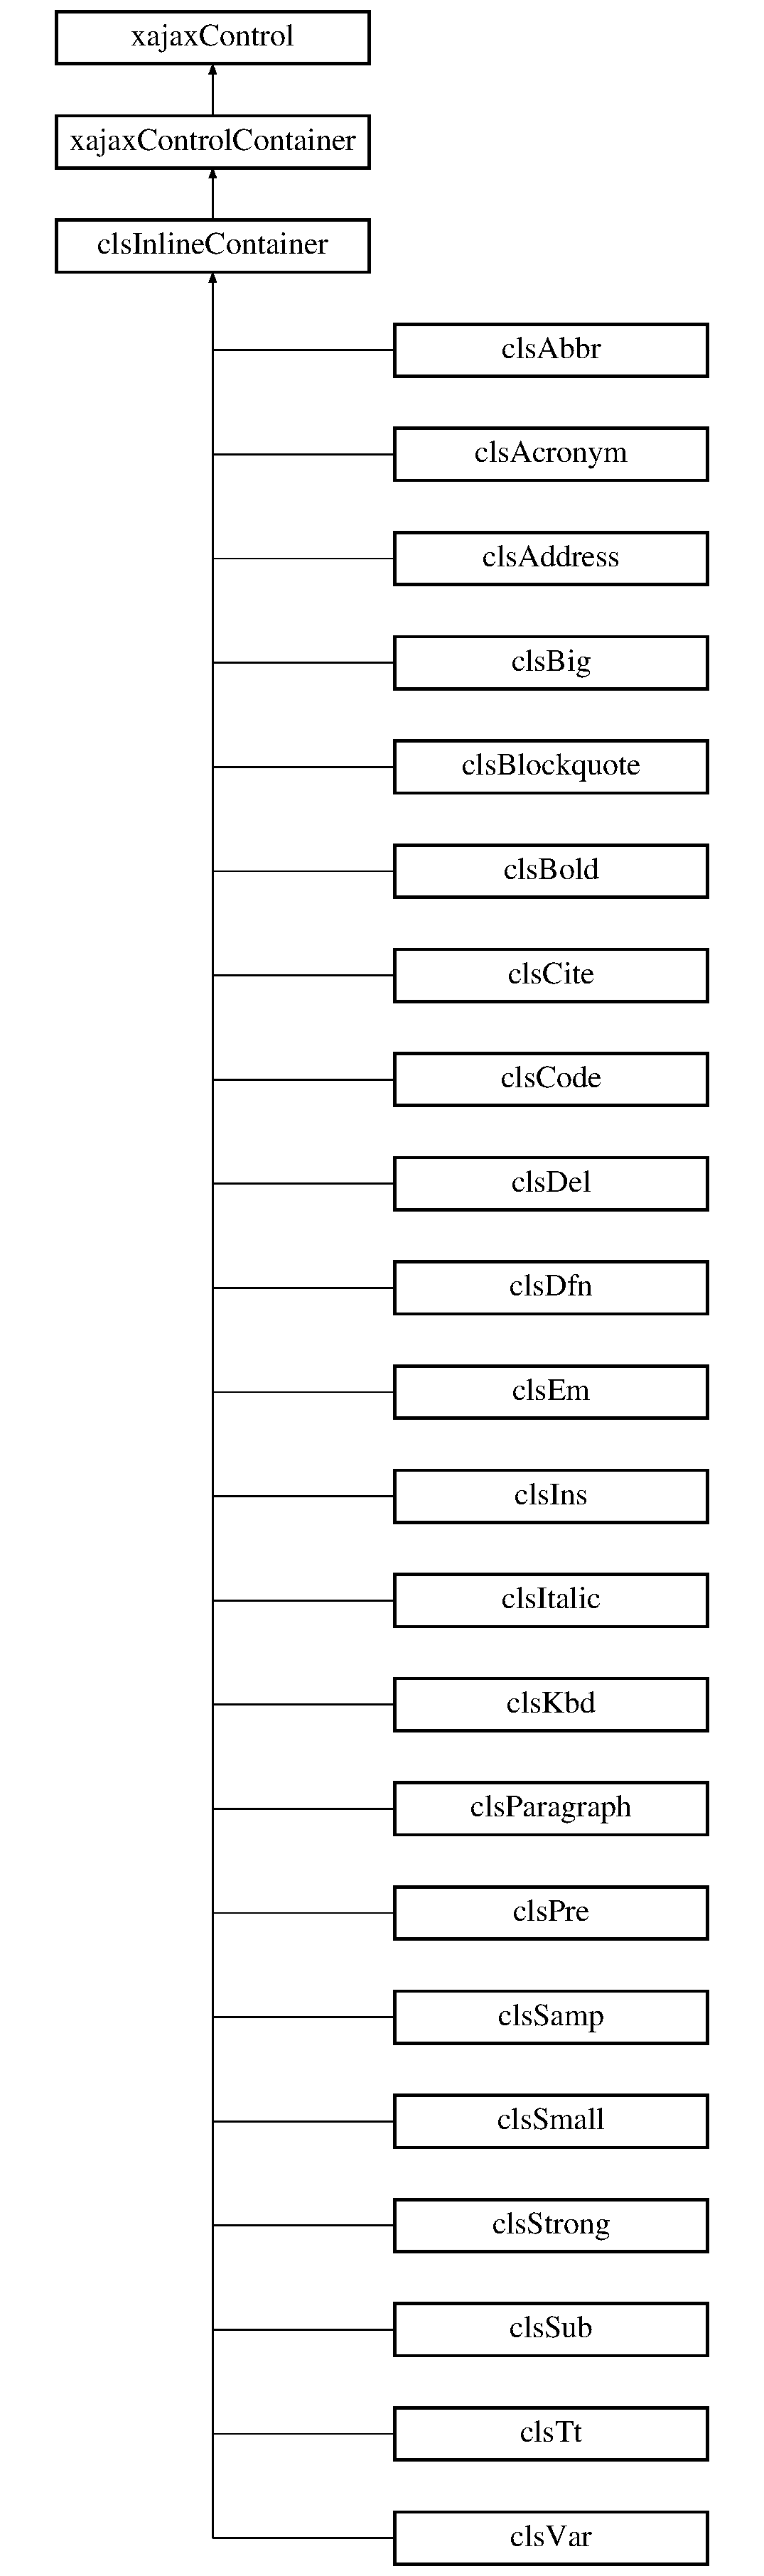
\includegraphics[height=12.000000cm]{classclsInlineContainer}
\end{center}
\end{figure}
\subsection*{Public Member Functions}
\begin{DoxyCompactItemize}
\item 
\hypertarget{classclsInlineContainer_ad0188701a5749da3222e0e52e6649487}{
{\bfseries clsInlineContainer} (\$sTag, \$aConfiguration)}
\label{classclsInlineContainer_ad0188701a5749da3222e0e52e6649487}

\end{DoxyCompactItemize}


\subsection{Detailed Description}


Definition at line 74 of file content.inc.php.



The documentation for this class was generated from the following file:\begin{DoxyCompactItemize}
\item 
xajax\_\-controls/content.inc.php\end{DoxyCompactItemize}

\hypertarget{classclsInput}{
\section{clsInput Class Reference}
\label{classclsInput}\index{clsInput@{clsInput}}
}
Inheritance diagram for clsInput:\begin{figure}[H]
\begin{center}
\leavevmode
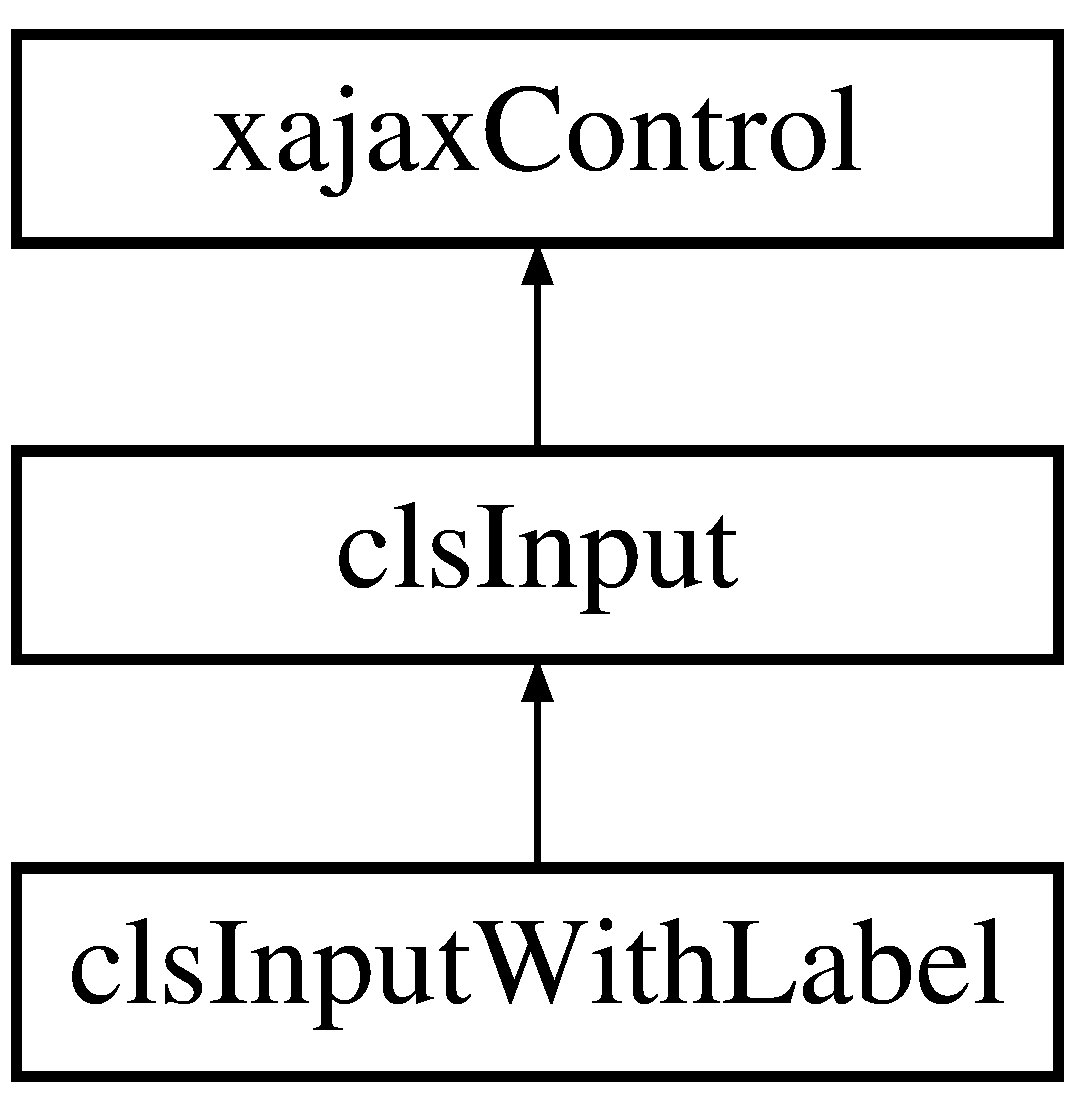
\includegraphics[height=3.000000cm]{classclsInput}
\end{center}
\end{figure}
\subsection*{Public Member Functions}
\begin{DoxyCompactItemize}
\item 
\hypertarget{classclsInput_a04fe27d3a5ba574d93c57779eea8bc78}{
{\bfseries clsInput} (\$aConfiguration=array())}
\label{classclsInput_a04fe27d3a5ba574d93c57779eea8bc78}

\end{DoxyCompactItemize}


\subsection{Detailed Description}


Definition at line 52 of file form.inc.php.



The documentation for this class was generated from the following file:\begin{DoxyCompactItemize}
\item 
xajax\_\-controls/form.inc.php\end{DoxyCompactItemize}

\hypertarget{classclsInputWithLabel}{
\section{clsInputWithLabel Class Reference}
\label{classclsInputWithLabel}\index{clsInputWithLabel@{clsInputWithLabel}}
}
Inheritance diagram for clsInputWithLabel:\begin{figure}[H]
\begin{center}
\leavevmode
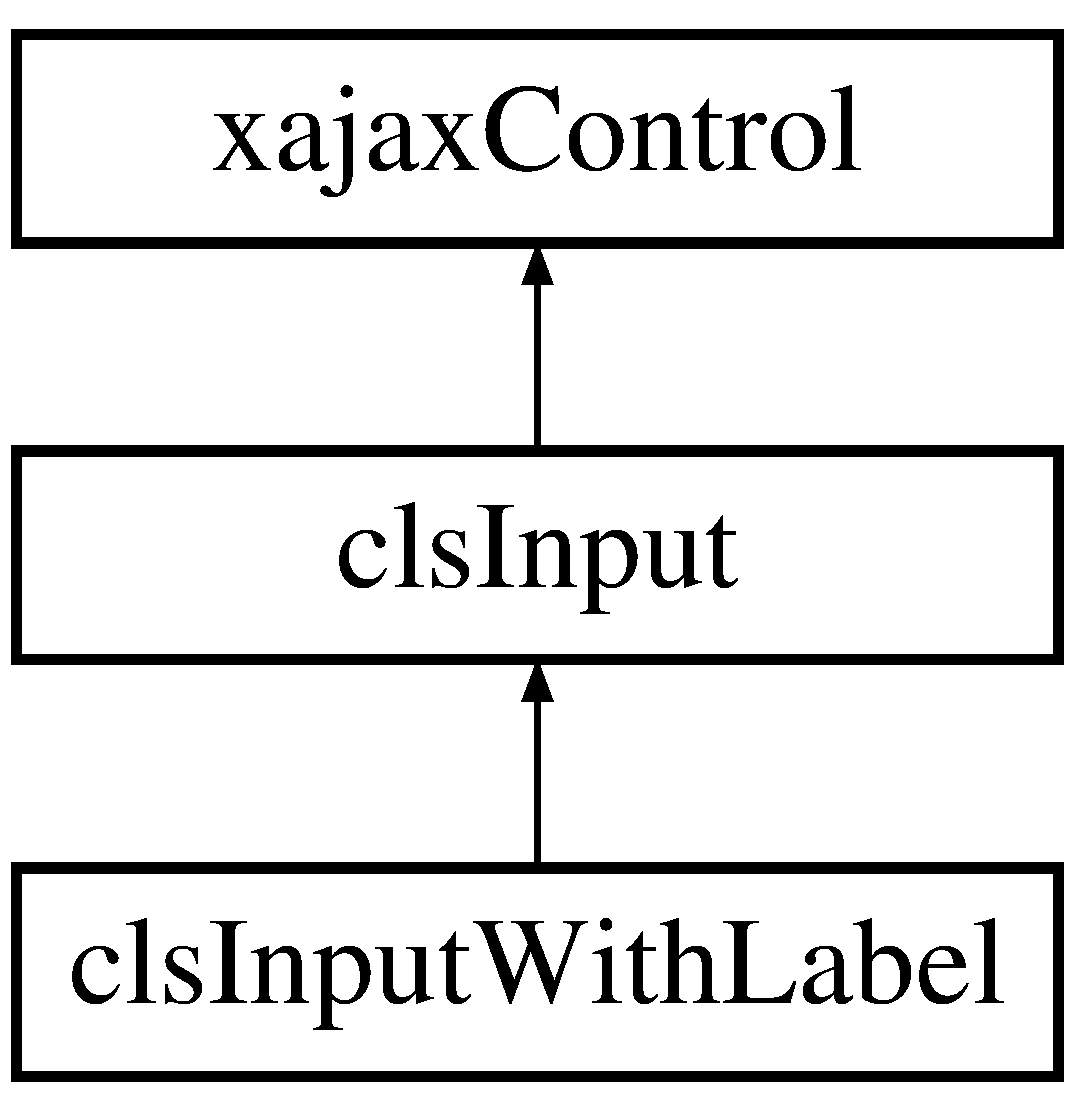
\includegraphics[height=3.000000cm]{classclsInputWithLabel}
\end{center}
\end{figure}
\subsection*{Public Member Functions}
\begin{DoxyCompactItemize}
\item 
\hypertarget{classclsInputWithLabel_abfd09670363cbcb8fee625edde801392}{
{\bfseries clsInputWithLabel} (\$sLabel, \$sWhere, \$aConfiguration=array())}
\label{classclsInputWithLabel_abfd09670363cbcb8fee625edde801392}

\item 
\hypertarget{classclsInputWithLabel_a0023f982fc0cb8cb8317812c17c5f9cf}{
{\bfseries printHTML} (\$sIndent='')}
\label{classclsInputWithLabel_a0023f982fc0cb8cb8317812c17c5f9cf}

\end{DoxyCompactItemize}
\subsection*{Public Attributes}
\begin{DoxyCompactItemize}
\item 
\hypertarget{classclsInputWithLabel_ae7301f1c2980344b70925cba5b5c7061}{
{\bfseries \$objLabel}}
\label{classclsInputWithLabel_ae7301f1c2980344b70925cba5b5c7061}

\item 
\hypertarget{classclsInputWithLabel_a661624736de18b2702074f99c0fd01d9}{
{\bfseries \$sWhere}}
\label{classclsInputWithLabel_a661624736de18b2702074f99c0fd01d9}

\item 
\hypertarget{classclsInputWithLabel_a6c5425456baad279bdc5362f7146bcff}{
{\bfseries \$objBreak}}
\label{classclsInputWithLabel_a6c5425456baad279bdc5362f7146bcff}

\end{DoxyCompactItemize}


\subsection{Detailed Description}


Definition at line 60 of file form.inc.php.



The documentation for this class was generated from the following file:\begin{DoxyCompactItemize}
\item 
xajax\_\-controls/form.inc.php\end{DoxyCompactItemize}

\hypertarget{classclsIns}{
\section{clsIns Class Reference}
\label{classclsIns}\index{clsIns@{clsIns}}
}
Inheritance diagram for clsIns:\begin{figure}[H]
\begin{center}
\leavevmode
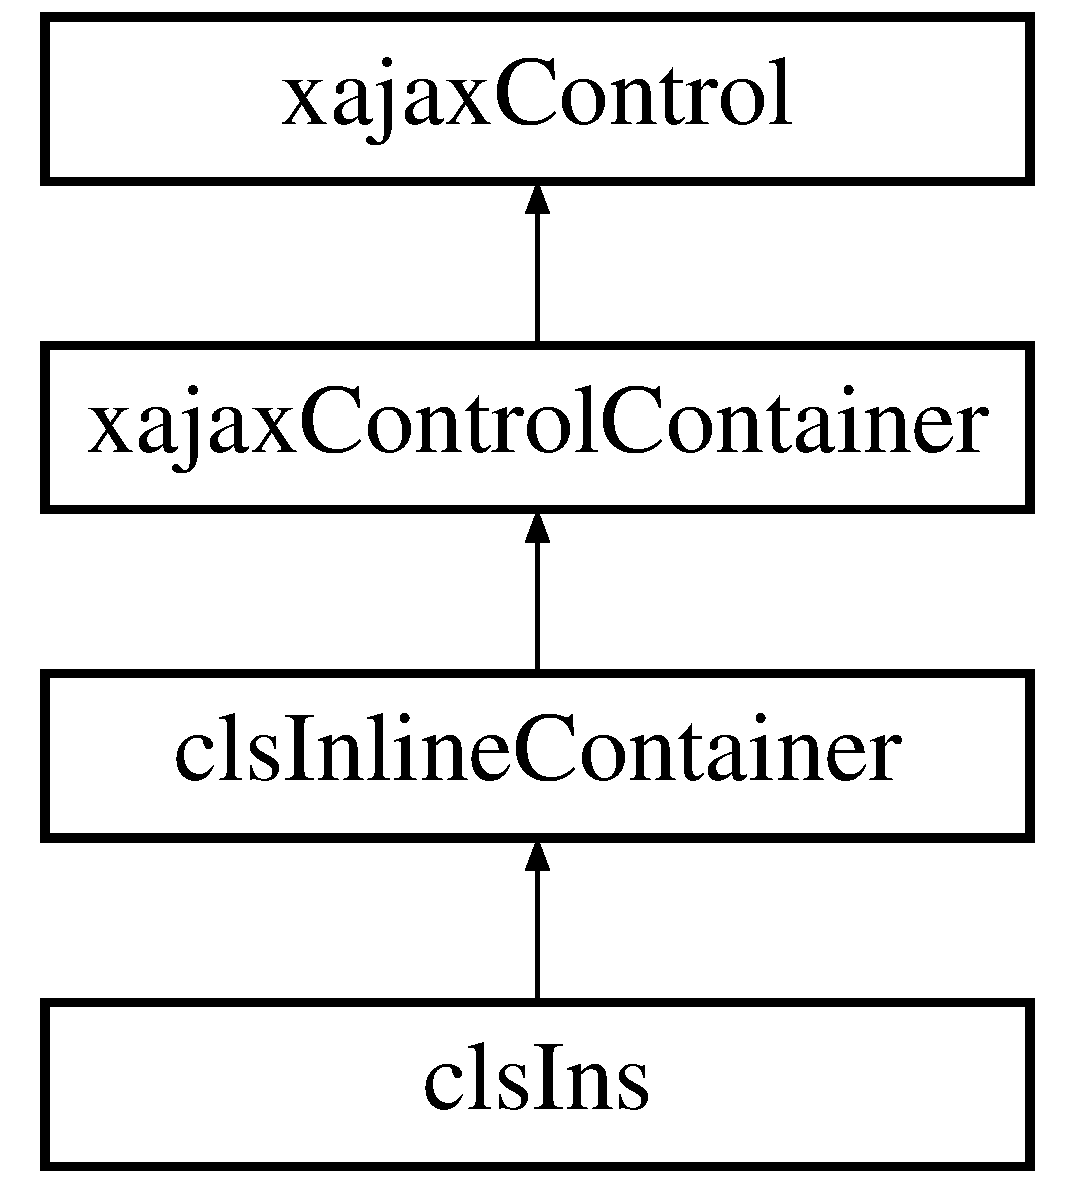
\includegraphics[height=4.000000cm]{classclsIns}
\end{center}
\end{figure}
\subsection*{Public Member Functions}
\begin{DoxyCompactItemize}
\item 
\hypertarget{classclsIns_a9af5593fa7172032d0da030f80b4f563}{
{\bfseries clsIns} (\$aConfiguration=array())}
\label{classclsIns_a9af5593fa7172032d0da030f80b4f563}

\end{DoxyCompactItemize}


\subsection{Detailed Description}


Definition at line 222 of file content.inc.php.



The documentation for this class was generated from the following file:\begin{DoxyCompactItemize}
\item 
xajax\_\-controls/content.inc.php\end{DoxyCompactItemize}

\hypertarget{classclsItalic}{
\section{clsItalic Class Reference}
\label{classclsItalic}\index{clsItalic@{clsItalic}}
}
Inheritance diagram for clsItalic:\begin{figure}[H]
\begin{center}
\leavevmode
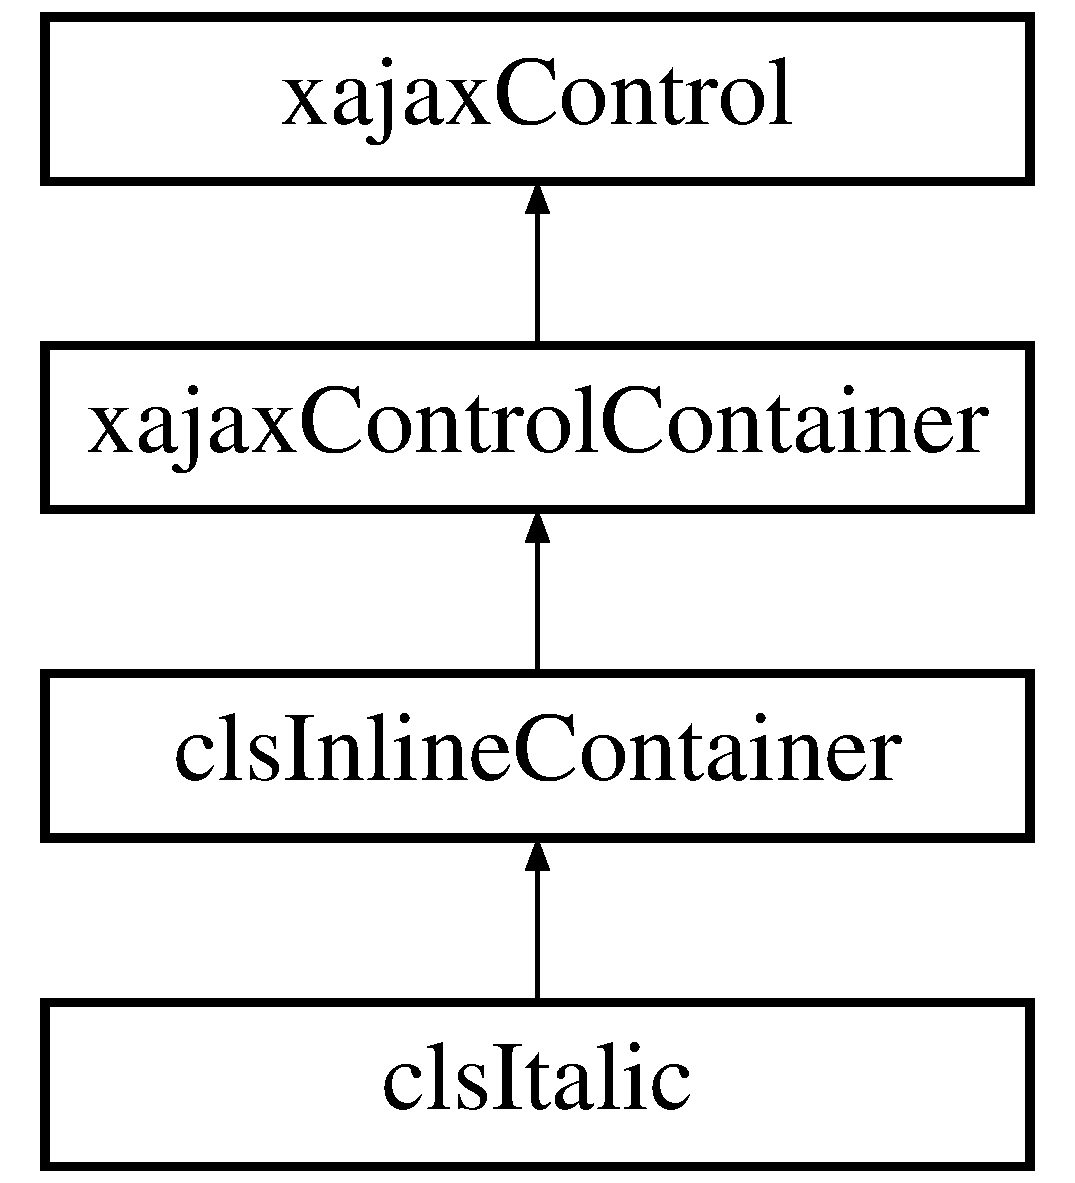
\includegraphics[height=4.000000cm]{classclsItalic}
\end{center}
\end{figure}
\subsection*{Public Member Functions}
\begin{DoxyCompactItemize}
\item 
\hypertarget{classclsItalic_a215a2a4beb43d0b65361bdad656acad5}{
{\bfseries clsItalic} (\$aConfiguration=array())}
\label{classclsItalic_a215a2a4beb43d0b65361bdad656acad5}

\end{DoxyCompactItemize}


\subsection{Detailed Description}


Definition at line 189 of file content.inc.php.



The documentation for this class was generated from the following file:\begin{DoxyCompactItemize}
\item 
xajax\_\-controls/content.inc.php\end{DoxyCompactItemize}

\hypertarget{classclsKbd}{
\section{clsKbd Class Reference}
\label{classclsKbd}\index{clsKbd@{clsKbd}}
}
Inheritance diagram for clsKbd:\begin{figure}[H]
\begin{center}
\leavevmode
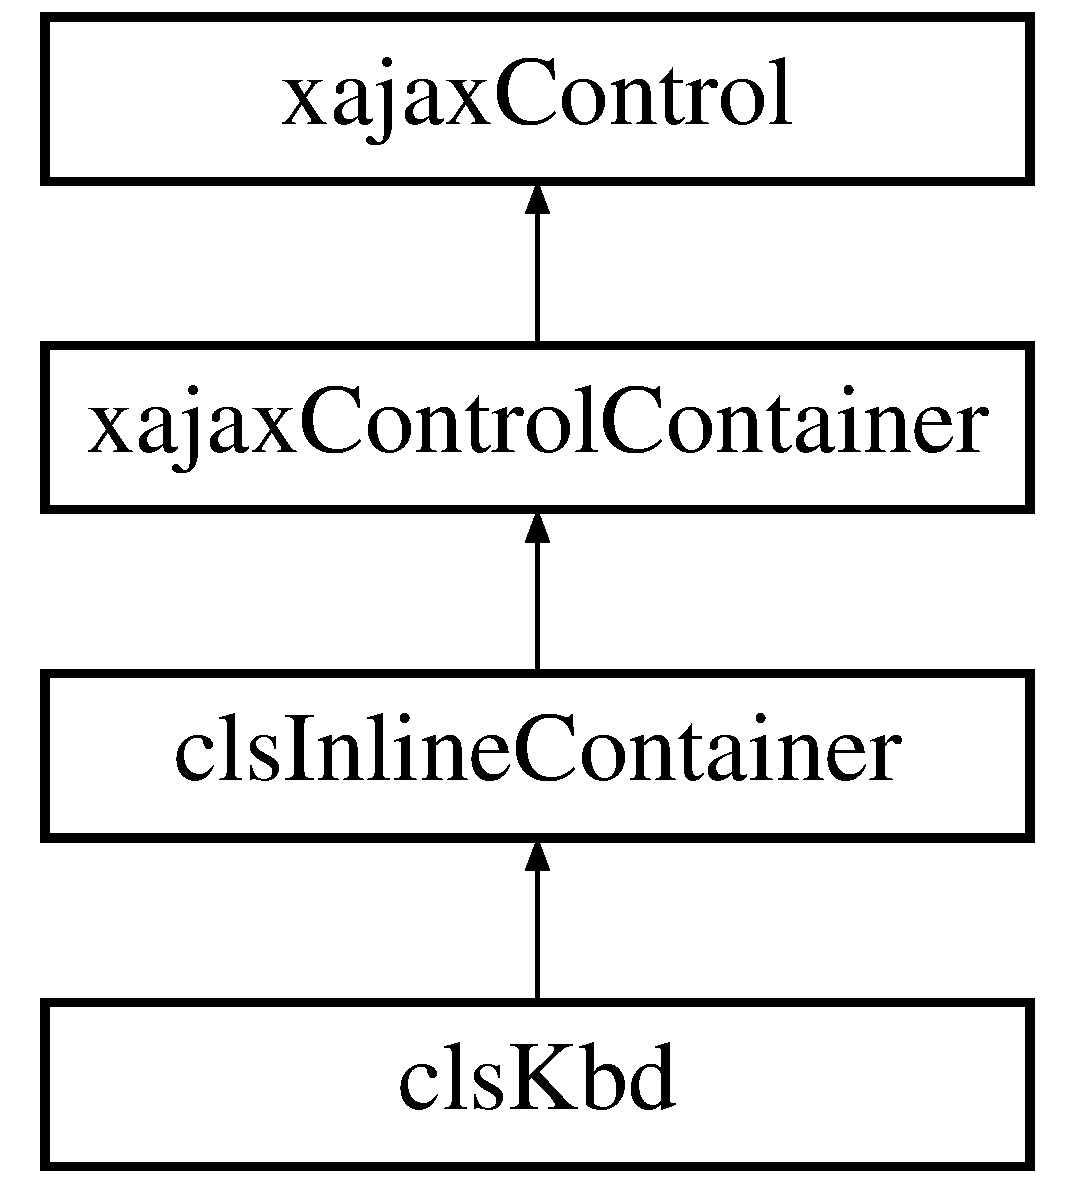
\includegraphics[height=4.000000cm]{classclsKbd}
\end{center}
\end{figure}
\subsection*{Public Member Functions}
\begin{DoxyCompactItemize}
\item 
\hypertarget{classclsKbd_a47731a6c5672f0fdfc0703fb737351c4}{
{\bfseries clsKbd} (\$aConfiguration=array())}
\label{classclsKbd_a47731a6c5672f0fdfc0703fb737351c4}

\end{DoxyCompactItemize}


\subsection{Detailed Description}


Definition at line 149 of file content.inc.php.



The documentation for this class was generated from the following file:\begin{DoxyCompactItemize}
\item 
xajax\_\-controls/content.inc.php\end{DoxyCompactItemize}

\hypertarget{classclsLabel}{
\section{clsLabel Class Reference}
\label{classclsLabel}\index{clsLabel@{clsLabel}}
}
Inheritance diagram for clsLabel:\begin{figure}[H]
\begin{center}
\leavevmode
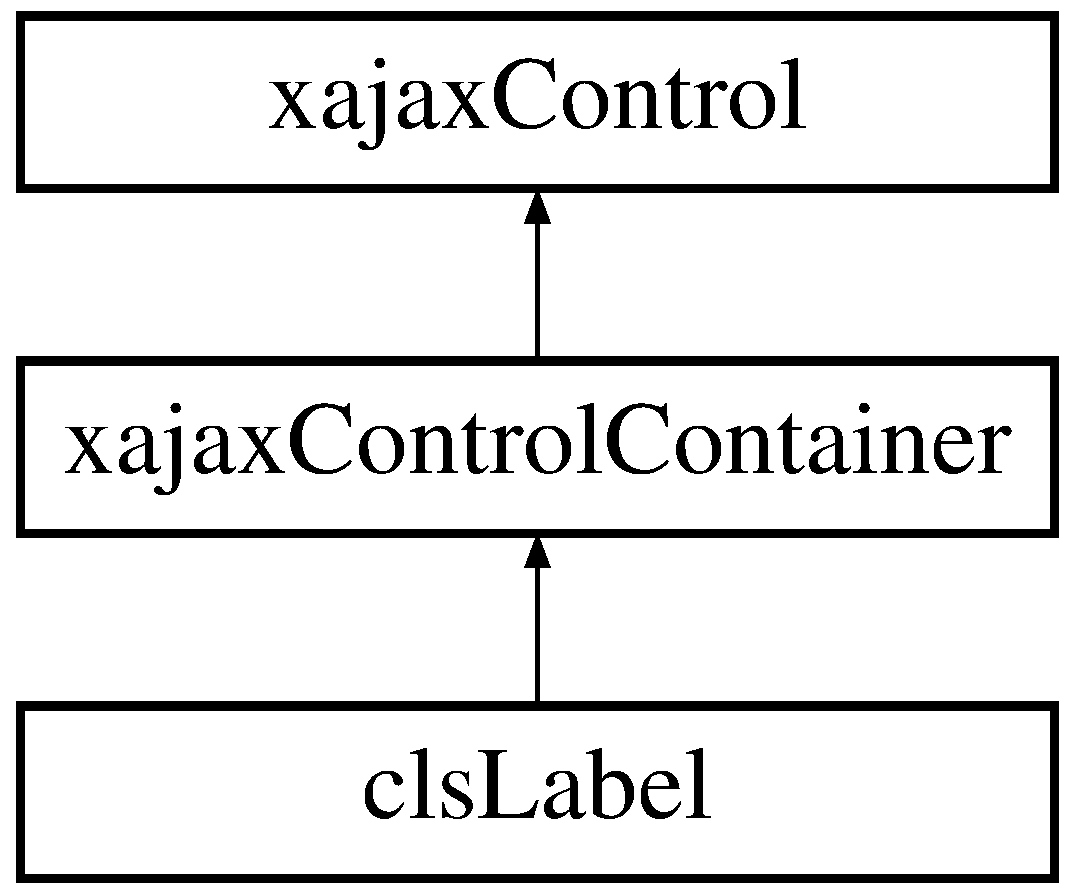
\includegraphics[height=3.000000cm]{classclsLabel}
\end{center}
\end{figure}
\subsection*{Public Member Functions}
\begin{DoxyCompactItemize}
\item 
\hypertarget{classclsLabel_a46d2704562c83935d036fd8e06f6f1d1}{
{\bfseries clsLabel} (\$aConfiguration=array())}
\label{classclsLabel_a46d2704562c83935d036fd8e06f6f1d1}

\item 
\hypertarget{classclsLabel_a00d6c5ad38575b8550e5d402e06b8e5f}{
{\bfseries setControl} (\&\$objControl)}
\label{classclsLabel_a00d6c5ad38575b8550e5d402e06b8e5f}

\item 
\hypertarget{classclsLabel_ab1bbc597d72c94b5e651950b6542b38c}{
{\bfseries printHTML} (\$sIndent='')}
\label{classclsLabel_ab1bbc597d72c94b5e651950b6542b38c}

\end{DoxyCompactItemize}
\subsection*{Public Attributes}
\begin{DoxyCompactItemize}
\item 
\hypertarget{classclsLabel_af97462aa53e20e675812d2d1e6fb9f43}{
{\bfseries \$objFor}}
\label{classclsLabel_af97462aa53e20e675812d2d1e6fb9f43}

\end{DoxyCompactItemize}


\subsection{Detailed Description}


Definition at line 269 of file form.inc.php.



The documentation for this class was generated from the following file:\begin{DoxyCompactItemize}
\item 
xajax\_\-controls/form.inc.php\end{DoxyCompactItemize}

\hypertarget{classclsLegend}{
\section{clsLegend Class Reference}
\label{classclsLegend}\index{clsLegend@{clsLegend}}
}
Inheritance diagram for clsLegend:\begin{figure}[H]
\begin{center}
\leavevmode
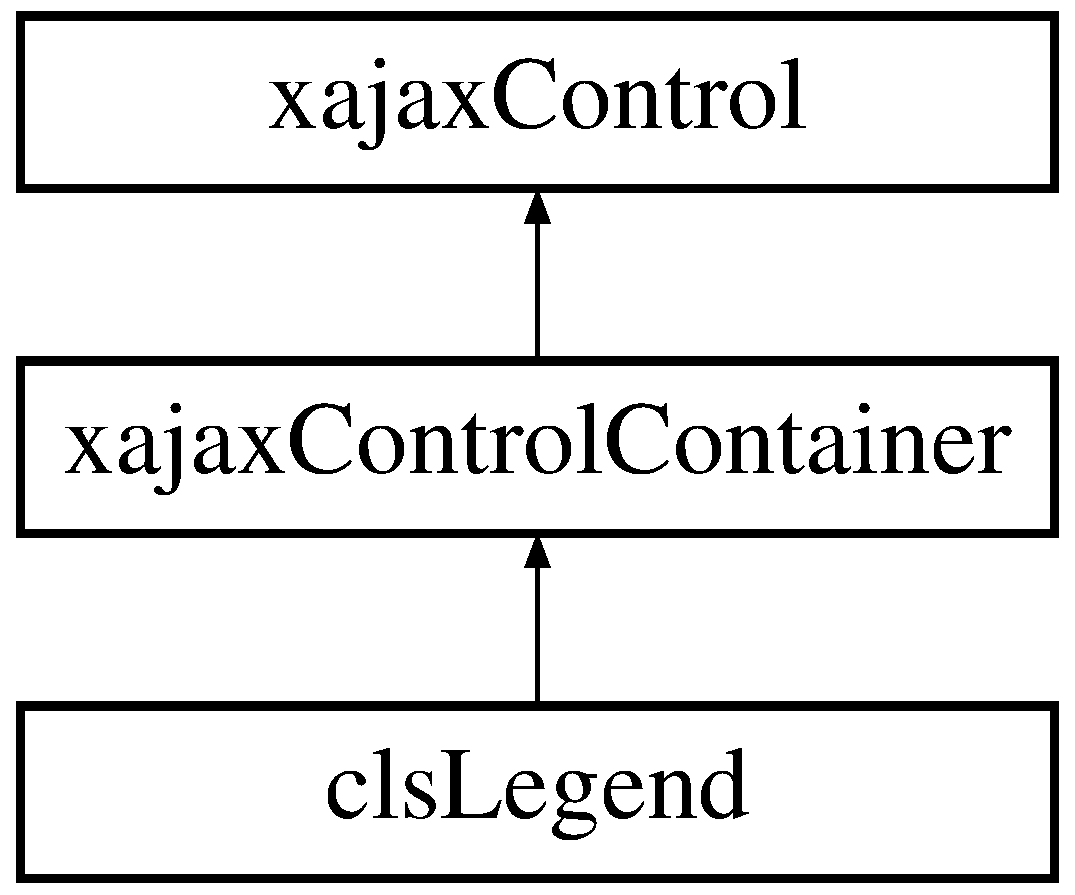
\includegraphics[height=3.000000cm]{classclsLegend}
\end{center}
\end{figure}
\subsection*{Public Member Functions}
\begin{DoxyCompactItemize}
\item 
\hypertarget{classclsLegend_a0de459add858edee6422bd3f0fa9a833}{
{\bfseries clsLegend} (\$aConfiguration=array())}
\label{classclsLegend_a0de459add858edee6422bd3f0fa9a833}

\end{DoxyCompactItemize}


\subsection{Detailed Description}


Definition at line 307 of file form.inc.php.



The documentation for this class was generated from the following file:\begin{DoxyCompactItemize}
\item 
xajax\_\-controls/form.inc.php\end{DoxyCompactItemize}

\hypertarget{classclsLI}{
\section{clsLI Class Reference}
\label{classclsLI}\index{clsLI@{clsLI}}
}
Inheritance diagram for clsLI:\begin{figure}[H]
\begin{center}
\leavevmode
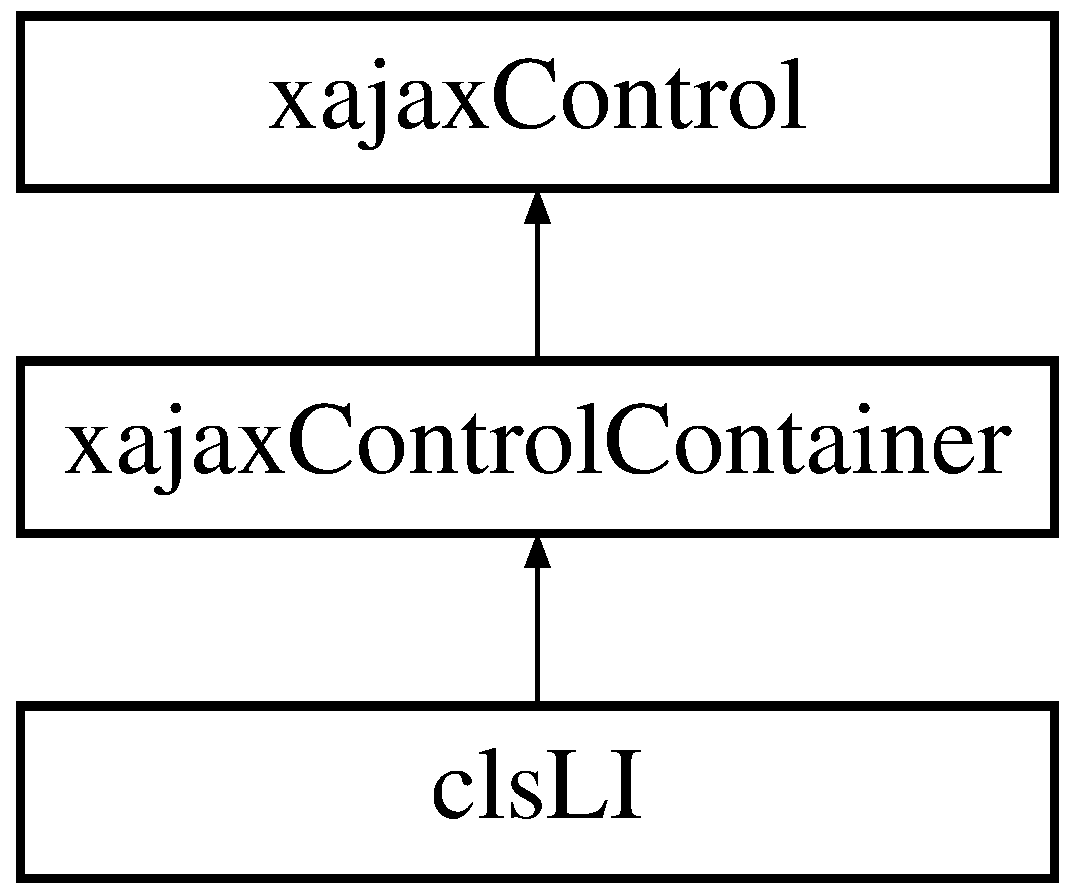
\includegraphics[height=3.000000cm]{classclsLI}
\end{center}
\end{figure}
\subsection*{Public Member Functions}
\begin{DoxyCompactItemize}
\item 
\hypertarget{classclsLI_a2f1557cc54a751f6874a81d18828b911}{
{\bfseries clsLI} (\$aConfiguration=array())}
\label{classclsLI_a2f1557cc54a751f6874a81d18828b911}

\end{DoxyCompactItemize}


\subsection{Detailed Description}


Definition at line 99 of file group.inc.php.



The documentation for this class was generated from the following file:\begin{DoxyCompactItemize}
\item 
xajax\_\-controls/group.inc.php\end{DoxyCompactItemize}

\hypertarget{classclsLink}{
\section{clsLink Class Reference}
\label{classclsLink}\index{clsLink@{clsLink}}
}
Inheritance diagram for clsLink:\begin{figure}[H]
\begin{center}
\leavevmode
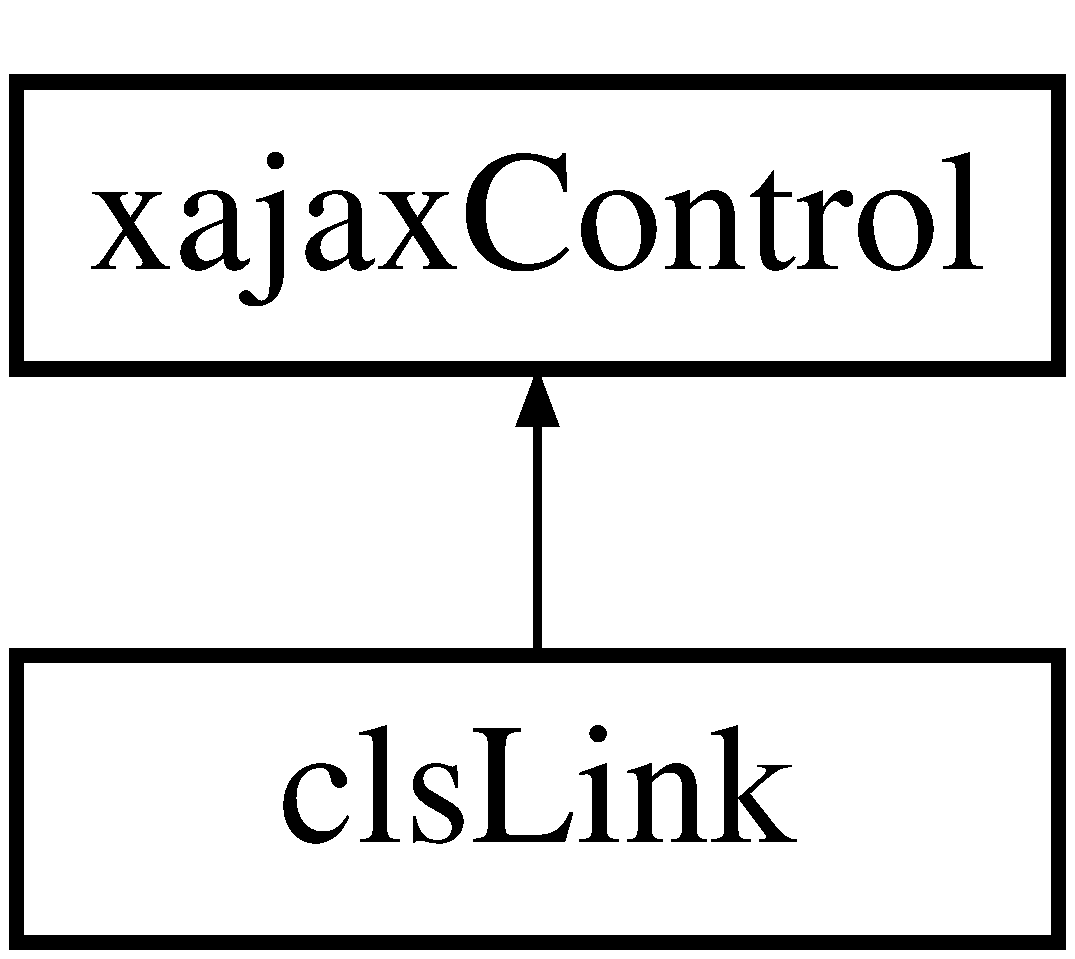
\includegraphics[height=2.000000cm]{classclsLink}
\end{center}
\end{figure}
\subsection*{Public Member Functions}
\begin{DoxyCompactItemize}
\item 
\hypertarget{classclsLink_a120fd3d895c7687e92a4f30d46cc1a23}{
{\bfseries clsLink} (\$aConfiguration=array())}
\label{classclsLink_a120fd3d895c7687e92a4f30d46cc1a23}

\end{DoxyCompactItemize}


\subsection{Detailed Description}


Definition at line 228 of file document.inc.php.



The documentation for this class was generated from the following file:\begin{DoxyCompactItemize}
\item 
xajax\_\-controls/document.inc.php\end{DoxyCompactItemize}

\hypertarget{classclsList}{
\section{clsList Class Reference}
\label{classclsList}\index{clsList@{clsList}}
}
Inheritance diagram for clsList:\begin{figure}[H]
\begin{center}
\leavevmode
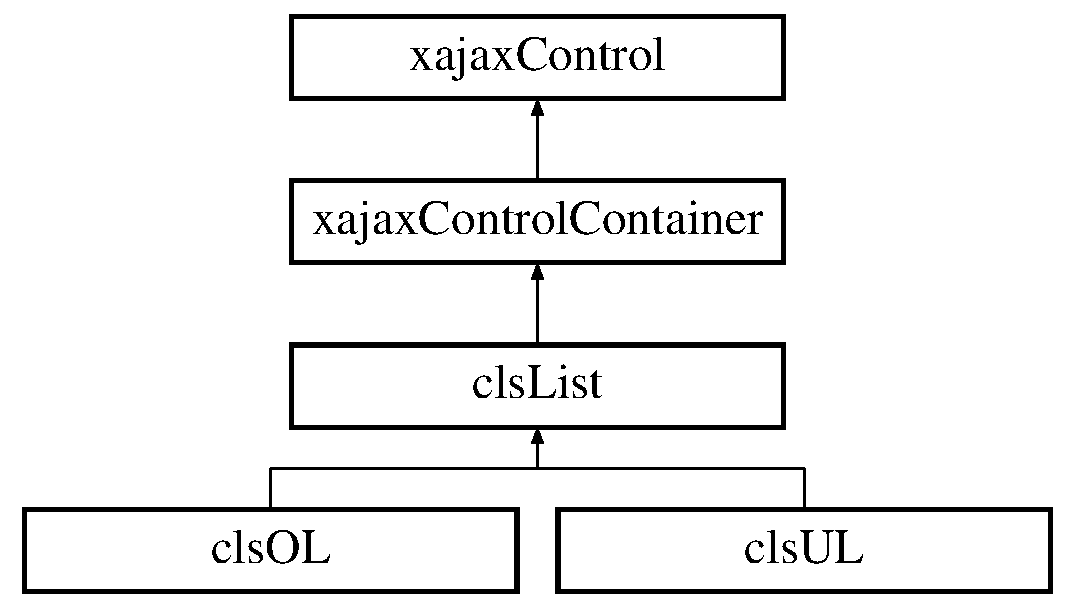
\includegraphics[height=4.000000cm]{classclsList}
\end{center}
\end{figure}
\subsection*{Public Member Functions}
\begin{DoxyCompactItemize}
\item 
\hypertarget{classclsList_a061cc0e9d713f527d76908f747474a51}{
{\bfseries clsList} (\$sTag, \$aConfiguration=array())}
\label{classclsList_a061cc0e9d713f527d76908f747474a51}

\item 
\hypertarget{classclsList_a7a2952c6565257e7830e919ff606475e}{
{\bfseries addItem} (\$mItem, \$mConfiguration=null)}
\label{classclsList_a7a2952c6565257e7830e919ff606475e}

\item 
\hypertarget{classclsList_a57250c3fe8febafbcf0c6b18e24047b5}{
{\bfseries addItems} (\$aItems, \$mConfiguration=null)}
\label{classclsList_a57250c3fe8febafbcf0c6b18e24047b5}

\item 
\hypertarget{classclsList_a0a22072328b60be67e223bbd6c76f942}{
{\bfseries clearEvent\_\-AddItem} ()}
\label{classclsList_a0a22072328b60be67e223bbd6c76f942}

\item 
\hypertarget{classclsList_abaf1f0c19c2ed96fb94189e2f1417738}{
{\bfseries setEvent\_\-AddItem} (\$mFunction)}
\label{classclsList_abaf1f0c19c2ed96fb94189e2f1417738}

\item 
\hypertarget{classclsList_a5500888d0364980cba3384a9cfc73524}{
\& {\bfseries \_\-onAddItem} (\$mItem, \$mConfiguration)}
\label{classclsList_a5500888d0364980cba3384a9cfc73524}

\end{DoxyCompactItemize}


\subsection{Detailed Description}


Definition at line 36 of file group.inc.php.



The documentation for this class was generated from the following file:\begin{DoxyCompactItemize}
\item 
xajax\_\-controls/group.inc.php\end{DoxyCompactItemize}

\hypertarget{classclsLiteral}{
\section{clsLiteral Class Reference}
\label{classclsLiteral}\index{clsLiteral@{clsLiteral}}
}
Inheritance diagram for clsLiteral:\begin{figure}[H]
\begin{center}
\leavevmode
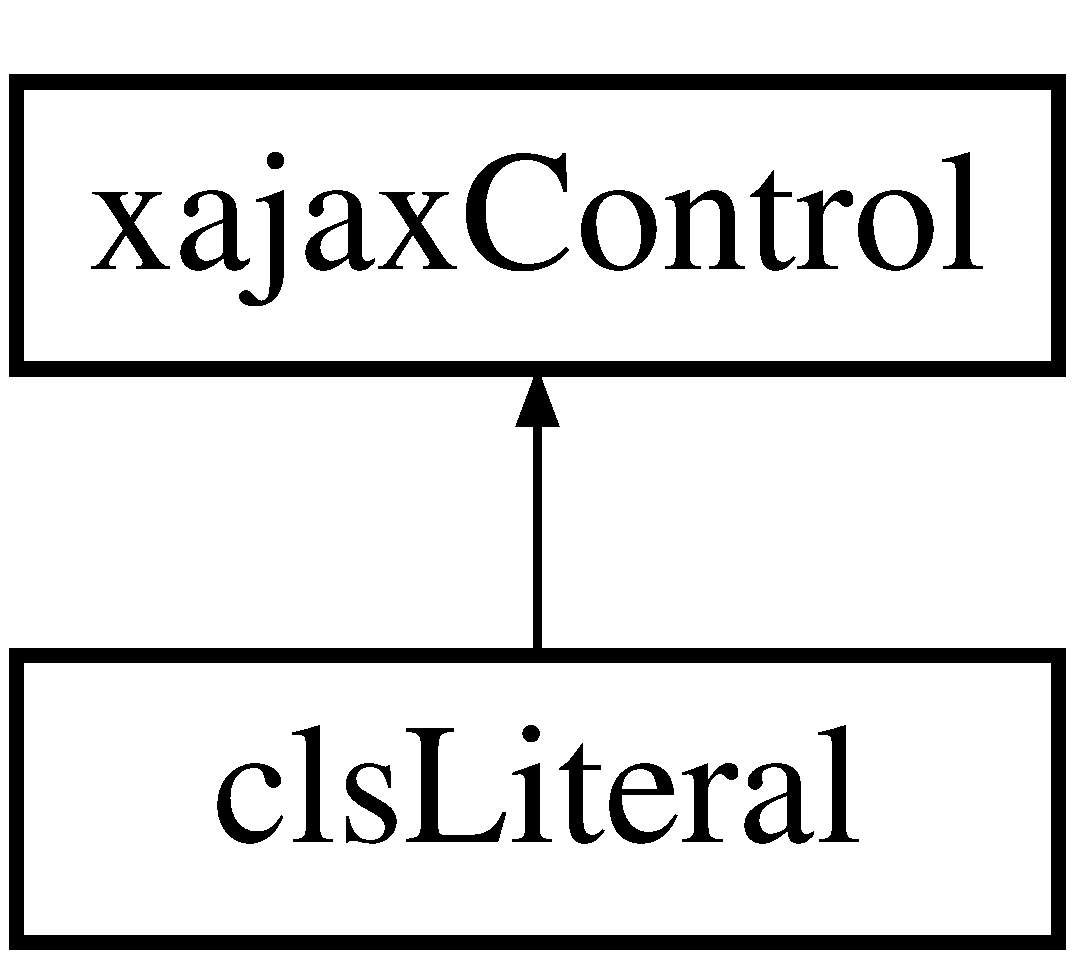
\includegraphics[height=2.000000cm]{classclsLiteral}
\end{center}
\end{figure}
\subsection*{Public Member Functions}
\begin{DoxyCompactItemize}
\item 
\hypertarget{classclsLiteral_ac1725d0d31c4df644b8fa4cca85b1021}{
{\bfseries clsLiteral} (\$sText)}
\label{classclsLiteral_ac1725d0d31c4df644b8fa4cca85b1021}

\item 
\hypertarget{classclsLiteral_adc4db95171e62fdd7b34d5b613e728ca}{
{\bfseries printHTML} (\$sIndent='')}
\label{classclsLiteral_adc4db95171e62fdd7b34d5b613e728ca}

\end{DoxyCompactItemize}


\subsection{Detailed Description}


Definition at line 36 of file content.inc.php.



The documentation for this class was generated from the following file:\begin{DoxyCompactItemize}
\item 
xajax\_\-controls/content.inc.php\end{DoxyCompactItemize}

\hypertarget{classclsMap}{
\section{clsMap Class Reference}
\label{classclsMap}\index{clsMap@{clsMap}}
}
Inheritance diagram for clsMap:\begin{figure}[H]
\begin{center}
\leavevmode
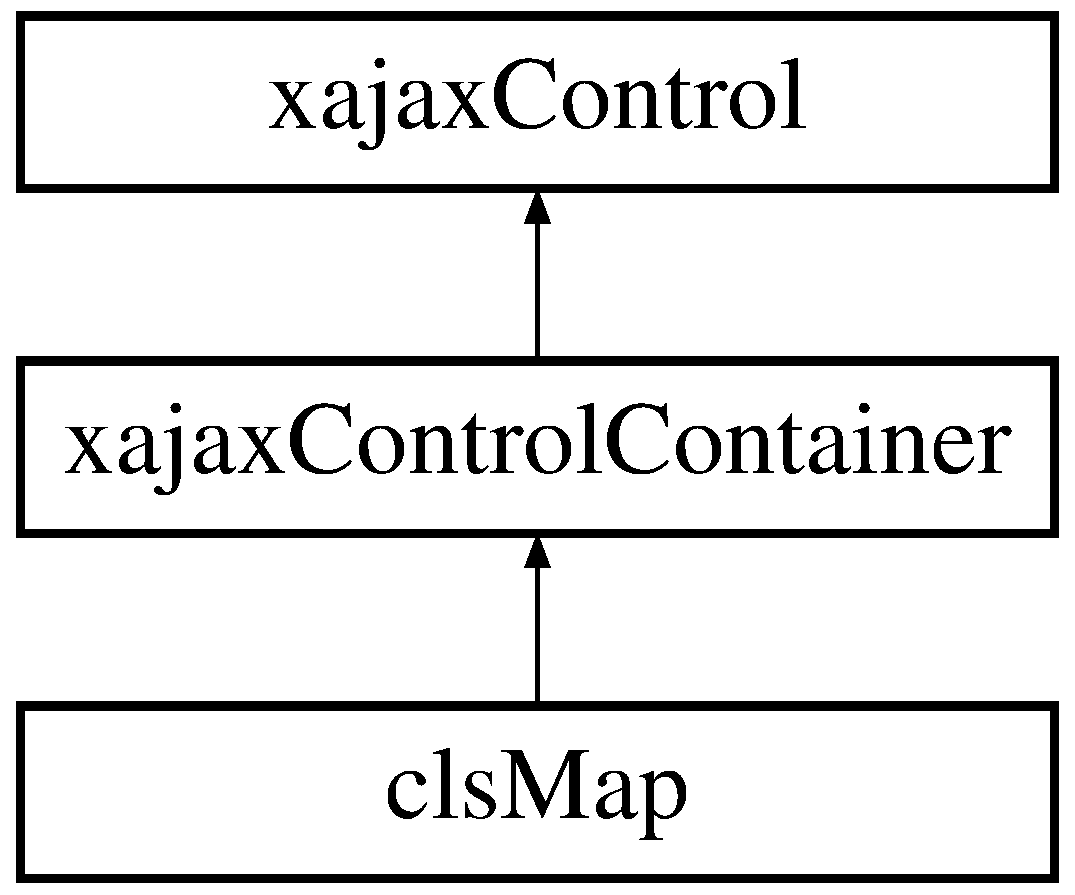
\includegraphics[height=3.000000cm]{classclsMap}
\end{center}
\end{figure}
\subsection*{Public Member Functions}
\begin{DoxyCompactItemize}
\item 
\hypertarget{classclsMap_ab8c244900e01a852ff254b9c4e9d0a10}{
{\bfseries clsMap} (\$aConfiguration=array())}
\label{classclsMap_ab8c244900e01a852ff254b9c4e9d0a10}

\end{DoxyCompactItemize}


\subsection{Detailed Description}


Definition at line 110 of file misc.inc.php.



The documentation for this class was generated from the following file:\begin{DoxyCompactItemize}
\item 
xajax\_\-controls/misc.inc.php\end{DoxyCompactItemize}

\hypertarget{classclsMeta}{
\section{clsMeta Class Reference}
\label{classclsMeta}\index{clsMeta@{clsMeta}}
}
Inheritance diagram for clsMeta:\begin{figure}[H]
\begin{center}
\leavevmode
\includegraphics[height=2.000000cm]{classclsMeta}
\end{center}
\end{figure}
\subsection*{Public Member Functions}
\begin{DoxyCompactItemize}
\item 
\hypertarget{classclsMeta_a1a28d98b3fa7a66aaa792ab884a4deea}{
{\bfseries clsMeta} (\$aConfiguration=array())}
\label{classclsMeta_a1a28d98b3fa7a66aaa792ab884a4deea}

\end{DoxyCompactItemize}


\subsection{Detailed Description}


Definition at line 238 of file document.inc.php.



The documentation for this class was generated from the following file:\begin{DoxyCompactItemize}
\item 
xajax\_\-controls/document.inc.php\end{DoxyCompactItemize}

\hypertarget{classclsMutuallyExclusiveButton}{
\section{clsMutuallyExclusiveButton Class Reference}
\label{classclsMutuallyExclusiveButton}\index{clsMutuallyExclusiveButton@{clsMutuallyExclusiveButton}}
}
Inheritance diagram for clsMutuallyExclusiveButton:\begin{figure}[H]
\begin{center}
\leavevmode
\includegraphics[height=2.000000cm]{classclsMutuallyExclusiveButton}
\end{center}
\end{figure}
\subsection*{Public Member Functions}
\begin{DoxyCompactItemize}
\item 
\hypertarget{classclsMutuallyExclusiveButton_a32679ecd8e5c7facae19c15f439ddf26}{
{\bfseries clsMutuallyExclusiveButton} (\$sId, \$sName, \$sValue)}
\label{classclsMutuallyExclusiveButton_a32679ecd8e5c7facae19c15f439ddf26}

\item 
\hypertarget{classclsMutuallyExclusiveButton_a0422dd0659b5bbb8cd4fc33c552a61e0}{
{\bfseries getId} ()}
\label{classclsMutuallyExclusiveButton_a0422dd0659b5bbb8cd4fc33c552a61e0}

\item 
\hypertarget{classclsMutuallyExclusiveButton_ad2ef33f1f1950052dcdacc776f0bb1d1}{
{\bfseries addPartner} (\&\$objPartnerNew)}
\label{classclsMutuallyExclusiveButton_ad2ef33f1f1950052dcdacc776f0bb1d1}

\item 
\hypertarget{classclsMutuallyExclusiveButton_a556e48f4b35ffa7f37158119f140e7ca}{
{\bfseries privateAddPartner} (\&\$objPartner)}
\label{classclsMutuallyExclusiveButton_a556e48f4b35ffa7f37158119f140e7ca}

\item 
\hypertarget{classclsMutuallyExclusiveButton_a28bfc24c148dd03f5be2a518830b277a}{
{\bfseries setAttribute} (\$sName, \$sValue)}
\label{classclsMutuallyExclusiveButton_a28bfc24c148dd03f5be2a518830b277a}

\item 
\hypertarget{classclsMutuallyExclusiveButton_ad5e4618a8df73baef6574de1d3bd0d75}{
{\bfseries printHtml} (\$sIndent='')}
\label{classclsMutuallyExclusiveButton_ad5e4618a8df73baef6574de1d3bd0d75}

\end{DoxyCompactItemize}
\subsection*{Public Attributes}
\begin{DoxyCompactItemize}
\item 
\hypertarget{classclsMutuallyExclusiveButton_a67a07aba937ad258a3723456e493212f}{
{\bfseries \$aPartners}}
\label{classclsMutuallyExclusiveButton_a67a07aba937ad258a3723456e493212f}

\end{DoxyCompactItemize}


\subsection{Detailed Description}


Definition at line 70 of file events.php.



The documentation for this class was generated from the following file:\begin{DoxyCompactItemize}
\item 
tests/suite/events.php\end{DoxyCompactItemize}

\hypertarget{classclsNoframes}{
\section{clsNoframes Class Reference}
\label{classclsNoframes}\index{clsNoframes@{clsNoframes}}
}
Inheritance diagram for clsNoframes:\begin{figure}[H]
\begin{center}
\leavevmode
\includegraphics[height=3.000000cm]{classclsNoframes}
\end{center}
\end{figure}
\subsection*{Public Member Functions}
\begin{DoxyCompactItemize}
\item 
\hypertarget{classclsNoframes_aeef91d8557446fbd56b0335ef2be15d1}{
{\bfseries clsNoframes} (\$aConfiguration=array())}
\label{classclsNoframes_aeef91d8557446fbd56b0335ef2be15d1}

\end{DoxyCompactItemize}


\subsection{Detailed Description}


Definition at line 316 of file document.inc.php.



The documentation for this class was generated from the following file:\begin{DoxyCompactItemize}
\item 
xajax\_\-controls/document.inc.php\end{DoxyCompactItemize}

\hypertarget{classclsNoscript}{
\section{clsNoscript Class Reference}
\label{classclsNoscript}\index{clsNoscript@{clsNoscript}}
}
Inheritance diagram for clsNoscript:\begin{figure}[H]
\begin{center}
\leavevmode
\includegraphics[height=3.000000cm]{classclsNoscript}
\end{center}
\end{figure}
\subsection*{Public Member Functions}
\begin{DoxyCompactItemize}
\item 
\hypertarget{classclsNoscript_ae56e3aa5701f902ca5b53fe797aeb49a}{
{\bfseries clsNoscript} (\$aConfiguration=array())}
\label{classclsNoscript_ae56e3aa5701f902ca5b53fe797aeb49a}

\end{DoxyCompactItemize}


\subsection{Detailed Description}


Definition at line 276 of file document.inc.php.



The documentation for this class was generated from the following file:\begin{DoxyCompactItemize}
\item 
xajax\_\-controls/document.inc.php\end{DoxyCompactItemize}

\hypertarget{classclsObject}{
\section{clsObject Class Reference}
\label{classclsObject}\index{clsObject@{clsObject}}
}
Inheritance diagram for clsObject:\begin{figure}[H]
\begin{center}
\leavevmode
\includegraphics[height=3.000000cm]{classclsObject}
\end{center}
\end{figure}
\subsection*{Public Member Functions}
\begin{DoxyCompactItemize}
\item 
\hypertarget{classclsObject_a57a9f5e2bd8fb2ea9183b72b5f772b1f}{
{\bfseries clsObject} (\$aConfiguration=array())}
\label{classclsObject_a57a9f5e2bd8fb2ea9183b72b5f772b1f}

\end{DoxyCompactItemize}


\subsection{Detailed Description}


Definition at line 38 of file misc.inc.php.



The documentation for this class was generated from the following file:\begin{DoxyCompactItemize}
\item 
xajax\_\-controls/misc.inc.php\end{DoxyCompactItemize}

\hypertarget{classclsOL}{
\section{clsOL Class Reference}
\label{classclsOL}\index{clsOL@{clsOL}}
}
Inheritance diagram for clsOL:\begin{figure}[H]
\begin{center}
\leavevmode
\includegraphics[height=4.000000cm]{classclsOL}
\end{center}
\end{figure}
\subsection*{Public Member Functions}
\begin{DoxyCompactItemize}
\item 
\hypertarget{classclsOL_ae53873e5db53a8844cf493172f72476c}{
{\bfseries clsOL} (\$aConfiguration=array())}
\label{classclsOL_ae53873e5db53a8844cf493172f72476c}

\end{DoxyCompactItemize}


\subsection{Detailed Description}


Definition at line 91 of file group.inc.php.



The documentation for this class was generated from the following file:\begin{DoxyCompactItemize}
\item 
xajax\_\-controls/group.inc.php\end{DoxyCompactItemize}

\hypertarget{classclsOption}{
\section{clsOption Class Reference}
\label{classclsOption}\index{clsOption@{clsOption}}
}
Inheritance diagram for clsOption:\begin{figure}[H]
\begin{center}
\leavevmode
\includegraphics[height=3.000000cm]{classclsOption}
\end{center}
\end{figure}
\subsection*{Public Member Functions}
\begin{DoxyCompactItemize}
\item 
\hypertarget{classclsOption_a64135332fe9010b582c4006099ee73a0}{
{\bfseries clsOption} (\$aConfiguration=array())}
\label{classclsOption_a64135332fe9010b582c4006099ee73a0}

\item 
\hypertarget{classclsOption_a313a9f6e423c66966f41305238803828}{
{\bfseries setValue} (\$sValue)}
\label{classclsOption_a313a9f6e423c66966f41305238803828}

\item 
\hypertarget{classclsOption_aef5713a971413b9fb362124853bc2b2c}{
{\bfseries setText} (\$sText)}
\label{classclsOption_aef5713a971413b9fb362124853bc2b2c}

\end{DoxyCompactItemize}


\subsection{Detailed Description}


Definition at line 222 of file form.inc.php.



The documentation for this class was generated from the following file:\begin{DoxyCompactItemize}
\item 
xajax\_\-controls/form.inc.php\end{DoxyCompactItemize}

\hypertarget{classclsOptionGroup}{
\section{clsOptionGroup Class Reference}
\label{classclsOptionGroup}\index{clsOptionGroup@{clsOptionGroup}}
}
Inheritance diagram for clsOptionGroup:\begin{figure}[H]
\begin{center}
\leavevmode
\includegraphics[height=3.000000cm]{classclsOptionGroup}
\end{center}
\end{figure}
\subsection*{Public Member Functions}
\begin{DoxyCompactItemize}
\item 
\hypertarget{classclsOptionGroup_a04ee61d6695114bd4aeb5b1e12f5ef8e}{
{\bfseries clsOptionGroup} (\$aConfiguration=array())}
\label{classclsOptionGroup_a04ee61d6695114bd4aeb5b1e12f5ef8e}

\item 
\hypertarget{classclsOptionGroup_a378828b3d483488cbffa062d272db6c7}{
{\bfseries addOption} (\$sValue, \$sText)}
\label{classclsOptionGroup_a378828b3d483488cbffa062d272db6c7}

\item 
\hypertarget{classclsOptionGroup_a17498edd6e697e1359eb0f4a07cc18ca}{
{\bfseries addOptions} (\$aOptions, \$aFields=array())}
\label{classclsOptionGroup_a17498edd6e697e1359eb0f4a07cc18ca}

\end{DoxyCompactItemize}


\subsection{Detailed Description}


Definition at line 165 of file form.inc.php.



The documentation for this class was generated from the following file:\begin{DoxyCompactItemize}
\item 
xajax\_\-controls/form.inc.php\end{DoxyCompactItemize}

\hypertarget{classclsPage}{
\section{clsPage Class Reference}
\label{classclsPage}\index{clsPage@{clsPage}}
}
\subsection*{Public Member Functions}
\begin{DoxyCompactItemize}
\item 
\hypertarget{classclsPage_a7570ae140bcbd468397dce3f68a106dc}{
{\bfseries clsPage} ()}
\label{classclsPage_a7570ae140bcbd468397dce3f68a106dc}

\item 
\hypertarget{classclsPage_aee2d974a8f93f271be051969d695da3a}{
{\bfseries sendAlert} (\$sValue)}
\label{classclsPage_aee2d974a8f93f271be051969d695da3a}

\item 
\hypertarget{classclsPage_a62dc75ca69b796a3432f400ea2c27715}{
{\bfseries sendConfirmCommands} ()}
\label{classclsPage_a62dc75ca69b796a3432f400ea2c27715}

\item 
\hypertarget{classclsPage_af1f2641cf9312df033e289e8718699e9}{
{\bfseries somePrivateFunction} ()}
\label{classclsPage_af1f2641cf9312df033e289e8718699e9}

\item 
\hypertarget{classclsPage_a9b079a6e0b081aaadd0791fac652972b}{
{\bfseries anotherPrivateFunction} ()}
\label{classclsPage_a9b079a6e0b081aaadd0791fac652972b}

\item 
\hypertarget{classclsPage_ae22140ebb3b6d1b3acb67e652a30ec1d}{
{\bfseries xajax\_\-public} ()}
\label{classclsPage_ae22140ebb3b6d1b3acb67e652a30ec1d}

\item 
\hypertarget{classclsPage_a48caf3088da64329eac9c3f96ec692a7}{
{\bfseries xajax\_\-private} ()}
\label{classclsPage_a48caf3088da64329eac9c3f96ec692a7}

\item 
\hypertarget{classclsPage_a7570ae140bcbd468397dce3f68a106dc}{
{\bfseries clsPage} ()}
\label{classclsPage_a7570ae140bcbd468397dce3f68a106dc}

\item 
\hypertarget{classclsPage_aaf09734e5363319e3a7fabda94b32d8b}{
{\bfseries sendAssignInnerHTML} ()}
\label{classclsPage_aaf09734e5363319e3a7fabda94b32d8b}

\item 
\hypertarget{classclsPage_a0315870b55719467ad885007a5693394}{
{\bfseries sendAssignStyleBackground} (\$color)}
\label{classclsPage_a0315870b55719467ad885007a5693394}

\item 
\hypertarget{classclsPage_af2a2482d6a1a3b2f6627ff81d4dc2cd1}{
{\bfseries sendAssignOuterHTML} ()}
\label{classclsPage_af2a2482d6a1a3b2f6627ff81d4dc2cd1}

\item 
\hypertarget{classclsPage_af3d458057796887f6970506d45cd8187}{
{\bfseries sendAppendInnerHTML} ()}
\label{classclsPage_af3d458057796887f6970506d45cd8187}

\item 
\hypertarget{classclsPage_a7570ae140bcbd468397dce3f68a106dc}{
{\bfseries clsPage} ()}
\label{classclsPage_a7570ae140bcbd468397dce3f68a106dc}

\item 
\hypertarget{classclsPage_a54096a4d02a62858f8ce2bfa2a4675ea}{
{\bfseries generateTable} ()}
\label{classclsPage_a54096a4d02a62858f8ce2bfa2a4675ea}

\item 
\hypertarget{classclsPage_af3a720187e19f18cbd207744b8c93aba}{
{\bfseries appendRow} ()}
\label{classclsPage_af3a720187e19f18cbd207744b8c93aba}

\item 
\hypertarget{classclsPage_ab144c6bc84640a0774b23d00a1f52d8d}{
{\bfseries insertRow} (\$old\_\-row)}
\label{classclsPage_ab144c6bc84640a0774b23d00a1f52d8d}

\item 
\hypertarget{classclsPage_a6b19998af7a5d64d8a484887d10f2dfc}{
{\bfseries replaceRow} (\$old\_\-row)}
\label{classclsPage_a6b19998af7a5d64d8a484887d10f2dfc}

\item 
\hypertarget{classclsPage_af9b2bcdd6306aae7d9f1a1a25ca2e11a}{
{\bfseries removeRow} (\$row)}
\label{classclsPage_af9b2bcdd6306aae7d9f1a1a25ca2e11a}

\item 
\hypertarget{classclsPage_af55540504f72e16ad42f35cbefaa23c5}{
{\bfseries setRowNumber} (\$row)}
\label{classclsPage_af55540504f72e16ad42f35cbefaa23c5}

\item 
\hypertarget{classclsPage_a49a7ab88742daab057077648306ccc4f}{
{\bfseries appendColumn} ()}
\label{classclsPage_a49a7ab88742daab057077648306ccc4f}

\item 
\hypertarget{classclsPage_ab4d81c6b088221ac03a2a3c0b19cd96d}{
{\bfseries insertColumn} (\$old\_\-column)}
\label{classclsPage_ab4d81c6b088221ac03a2a3c0b19cd96d}

\item 
\hypertarget{classclsPage_ac1c6b7aac1cf3003c58c5146631b6fea}{
{\bfseries replaceColumn} (\$old\_\-column)}
\label{classclsPage_ac1c6b7aac1cf3003c58c5146631b6fea}

\item 
\hypertarget{classclsPage_ae6f0cd72648a617ea7ea310cc0bac901}{
{\bfseries removeColumn} (\$column)}
\label{classclsPage_ae6f0cd72648a617ea7ea310cc0bac901}

\item 
\hypertarget{classclsPage_a92f0d2ab81862fadf63cd0840070770b}{
{\bfseries setColumnNumber} (\$column)}
\label{classclsPage_a92f0d2ab81862fadf63cd0840070770b}

\item 
\hypertarget{classclsPage_addef5bd69436a52d31a7dfa540539c41}{
{\bfseries setCellValue} (\$row, \$column, \$value)}
\label{classclsPage_addef5bd69436a52d31a7dfa540539c41}

\item 
\hypertarget{classclsPage_a6abbc411a311d9d72de0755c48ec932f}{
{\bfseries setCellProperty} (\$row, \$column, \$property, \$value)}
\label{classclsPage_a6abbc411a311d9d72de0755c48ec932f}

\item 
\hypertarget{classclsPage_a0b77ab4280a0d4efd5be597d490f6c66}{
{\bfseries setRowProperty} (\$row, \$property, \$value)}
\label{classclsPage_a0b77ab4280a0d4efd5be597d490f6c66}

\item 
\hypertarget{classclsPage_a4fea6ac11ec887303142f367b8176ea0}{
{\bfseries setColumnProperty} (\$column, \$property, \$value)}
\label{classclsPage_a4fea6ac11ec887303142f367b8176ea0}

\end{DoxyCompactItemize}


\subsection{Detailed Description}


Definition at line 39 of file alert\_\-confirm.php.



The documentation for this class was generated from the following files:\begin{DoxyCompactItemize}
\item 
tests/suite/alert\_\-confirm.php\item 
tests/suite/assign\_\-append.php\item 
tests/suite/tables.php\end{DoxyCompactItemize}

\hypertarget{classclsParagraph}{
\section{clsParagraph Class Reference}
\label{classclsParagraph}\index{clsParagraph@{clsParagraph}}
}
Inheritance diagram for clsParagraph:\begin{figure}[H]
\begin{center}
\leavevmode
\includegraphics[height=4.000000cm]{classclsParagraph}
\end{center}
\end{figure}
\subsection*{Public Member Functions}
\begin{DoxyCompactItemize}
\item 
\hypertarget{classclsParagraph_a2f52d411d6599f5453b7c823d26d36a3}{
{\bfseries clsParagraph} (\$aConfiguration=array())}
\label{classclsParagraph_a2f52d411d6599f5453b7c823d26d36a3}

\end{DoxyCompactItemize}


\subsection{Detailed Description}


Definition at line 262 of file content.inc.php.



The documentation for this class was generated from the following file:\begin{DoxyCompactItemize}
\item 
xajax\_\-controls/content.inc.php\end{DoxyCompactItemize}

\hypertarget{classclsParam}{
\section{clsParam Class Reference}
\label{classclsParam}\index{clsParam@{clsParam}}
}
Inheritance diagram for clsParam:\begin{figure}[H]
\begin{center}
\leavevmode
\includegraphics[height=2.000000cm]{classclsParam}
\end{center}
\end{figure}
\subsection*{Public Member Functions}
\begin{DoxyCompactItemize}
\item 
\hypertarget{classclsParam_a5c7634cb36819d00d3577ac5fda93200}{
{\bfseries clsParam} (\$aConfiguration=array())}
\label{classclsParam_a5c7634cb36819d00d3577ac5fda93200}

\end{DoxyCompactItemize}


\subsection{Detailed Description}


Definition at line 49 of file misc.inc.php.



The documentation for this class was generated from the following file:\begin{DoxyCompactItemize}
\item 
xajax\_\-controls/misc.inc.php\end{DoxyCompactItemize}

\hypertarget{classclsPre}{
\section{clsPre Class Reference}
\label{classclsPre}\index{clsPre@{clsPre}}
}
Inheritance diagram for clsPre:\begin{figure}[H]
\begin{center}
\leavevmode
\includegraphics[height=4.000000cm]{classclsPre}
\end{center}
\end{figure}
\subsection*{Public Member Functions}
\begin{DoxyCompactItemize}
\item 
\hypertarget{classclsPre_a799bdf5023afeb722b83571cf5471a56}{
{\bfseries clsPre} (\$aConfiguration=array())}
\label{classclsPre_a799bdf5023afeb722b83571cf5471a56}

\end{DoxyCompactItemize}


\subsection{Detailed Description}


Definition at line 278 of file content.inc.php.



The documentation for this class was generated from the following file:\begin{DoxyCompactItemize}
\item 
xajax\_\-controls/content.inc.php\end{DoxyCompactItemize}

\hypertarget{classclsRequests}{
\section{clsRequests Class Reference}
\label{classclsRequests}\index{clsRequests@{clsRequests}}
}
\subsection*{Public Member Functions}
\begin{DoxyCompactItemize}
\item 
\hypertarget{classclsRequests_abf00e5456c1624acca683a3f1584bd13}{
{\bfseries clsRequests} ()}
\label{classclsRequests_abf00e5456c1624acca683a3f1584bd13}

\item 
\hypertarget{classclsRequests_a9b517bdeb746d53e9567928b037f5dd0}{
{\bfseries clearLog} ()}
\label{classclsRequests_a9b517bdeb746d53e9567928b037f5dd0}

\item 
\hypertarget{classclsRequests_a6720963b04c8d0e9e00a427a7b3bcf33}{
{\bfseries shortDelay} (\$sleepTimes)}
\label{classclsRequests_a6720963b04c8d0e9e00a427a7b3bcf33}

\item 
\hypertarget{classclsRequests_ae0be0247b54a46bc726e27d59b0e31ad}{
{\bfseries mediumDelay} (\$sleepTimes)}
\label{classclsRequests_ae0be0247b54a46bc726e27d59b0e31ad}

\item 
\hypertarget{classclsRequests_a00e91c2cd430ad3cfbb4c5f7deb129d8}{
{\bfseries longDelay} ()}
\label{classclsRequests_a00e91c2cd430ad3cfbb4c5f7deb129d8}

\item 
\hypertarget{classclsRequests_a9b6374f3890ed20cb6fa703dc880c118}{
{\bfseries shortDelayS} ()}
\label{classclsRequests_a9b6374f3890ed20cb6fa703dc880c118}

\item 
\hypertarget{classclsRequests_ad721ac678548e8183e719d4b2fc8b53a}{
{\bfseries mediumDelayS} ()}
\label{classclsRequests_ad721ac678548e8183e719d4b2fc8b53a}

\item 
\hypertarget{classclsRequests_a119a98f418f09aa2add72503a4a21afe}{
{\bfseries longDelayS} ()}
\label{classclsRequests_a119a98f418f09aa2add72503a4a21afe}

\item 
\hypertarget{classclsRequests_abf00e5456c1624acca683a3f1584bd13}{
{\bfseries clsRequests} ()}
\label{classclsRequests_abf00e5456c1624acca683a3f1584bd13}

\item 
\hypertarget{classclsRequests_aefe0f19e2defb6061e760234f1917ba5}{
{\bfseries insertFunction} ()}
\label{classclsRequests_aefe0f19e2defb6061e760234f1917ba5}

\item 
\hypertarget{classclsRequests_afabd1b7dba58f75895e8fb9b5a83bf74}{
{\bfseries wrapFunction} ()}
\label{classclsRequests_afabd1b7dba58f75895e8fb9b5a83bf74}

\item 
\hypertarget{classclsRequests_ae243937177255fa0de65c9c7eba72335}{
{\bfseries deleteFunction} ()}
\label{classclsRequests_ae243937177255fa0de65c9c7eba72335}

\item 
\hypertarget{classclsRequests_a431c043ef017a22eadfe3abf18c07098}{
{\bfseries callFunction} ()}
\label{classclsRequests_a431c043ef017a22eadfe3abf18c07098}

\item 
\hypertarget{classclsRequests_abf00e5456c1624acca683a3f1584bd13}{
{\bfseries clsRequests} ()}
\label{classclsRequests_abf00e5456c1624acca683a3f1584bd13}

\item 
\hypertarget{classclsRequests_a92f4abbd473ee95778cf87dc901e8b67}{
{\bfseries loadTests} ()}
\label{classclsRequests_a92f4abbd473ee95778cf87dc901e8b67}

\item 
\hypertarget{classclsRequests_a80f55b2c0599bafb3e89c34ae862e1a2}{
{\bfseries nextTest} (\$values)}
\label{classclsRequests_a80f55b2c0599bafb3e89c34ae862e1a2}

\item 
\hypertarget{classclsRequests_acaa084d94af99c1e3bfffaef1d17bf3d}{
{\bfseries recompressJavascript} ()}
\label{classclsRequests_acaa084d94af99c1e3bfffaef1d17bf3d}

\item 
\hypertarget{classclsRequests_ac4fb35429664d8a889b98a2656a13906}{
{\bfseries recompileCore} ()}
\label{classclsRequests_ac4fb35429664d8a889b98a2656a13906}

\item 
\hypertarget{classclsRequests_a653b2eae1dca72895ec909d548f873a1}{
{\bfseries gotoTest} (\$values)}
\label{classclsRequests_a653b2eae1dca72895ec909d548f873a1}

\item 
\hypertarget{classclsRequests_a7e9dbc4e37eb66154c46283bf8448c11}{
{\bfseries toggleControlPanel} (\$bControlPanelVisible)}
\label{classclsRequests_a7e9dbc4e37eb66154c46283bf8448c11}

\end{DoxyCompactItemize}
\subsection*{Public Attributes}
\begin{DoxyCompactItemize}
\item 
\hypertarget{classclsRequests_ae521025ac891c847910ebb47b3fad90f}{
{\bfseries \$tests} = array()}
\label{classclsRequests_ae521025ac891c847910ebb47b3fad90f}

\end{DoxyCompactItemize}


\subsection{Detailed Description}


Definition at line 14 of file delayEvents.php.



The documentation for this class was generated from the following files:\begin{DoxyCompactItemize}
\item 
tests/suite/delayEvents.php\item 
tests/suite/index.php\item 
tests/suite/functions.php\end{DoxyCompactItemize}

\hypertarget{classclsSamp}{
\section{clsSamp Class Reference}
\label{classclsSamp}\index{clsSamp@{clsSamp}}
}
Inheritance diagram for clsSamp:\begin{figure}[H]
\begin{center}
\leavevmode
\includegraphics[height=4.000000cm]{classclsSamp}
\end{center}
\end{figure}
\subsection*{Public Member Functions}
\begin{DoxyCompactItemize}
\item 
\hypertarget{classclsSamp_a9f8216128c7b4ed441a8c8f5fe2c2c12}{
{\bfseries clsSamp} (\$aConfiguration=array())}
\label{classclsSamp_a9f8216128c7b4ed441a8c8f5fe2c2c12}

\end{DoxyCompactItemize}


\subsection{Detailed Description}


Definition at line 141 of file content.inc.php.



The documentation for this class was generated from the following file:\begin{DoxyCompactItemize}
\item 
xajax\_\-controls/content.inc.php\end{DoxyCompactItemize}

\hypertarget{classclsScript}{
\section{clsScript Class Reference}
\label{classclsScript}\index{clsScript@{clsScript}}
}
Inheritance diagram for clsScript:\begin{figure}[H]
\begin{center}
\leavevmode
\includegraphics[height=3.000000cm]{classclsScript}
\end{center}
\end{figure}
\subsection*{Public Member Functions}
\begin{DoxyCompactItemize}
\item 
\hypertarget{classclsScript_aa931c3e2cedc66fab55a9da9290f5f8a}{
{\bfseries clsScript} (\$aConfiguration=array())}
\label{classclsScript_aa931c3e2cedc66fab55a9da9290f5f8a}

\end{DoxyCompactItemize}


\subsection{Detailed Description}


Definition at line 208 of file document.inc.php.



The documentation for this class was generated from the following file:\begin{DoxyCompactItemize}
\item 
xajax\_\-controls/document.inc.php\end{DoxyCompactItemize}

\hypertarget{classclsSelect}{
\section{clsSelect Class Reference}
\label{classclsSelect}\index{clsSelect@{clsSelect}}
}
Inheritance diagram for clsSelect:\begin{figure}[H]
\begin{center}
\leavevmode
\includegraphics[height=3.000000cm]{classclsSelect}
\end{center}
\end{figure}
\subsection*{Public Member Functions}
\begin{DoxyCompactItemize}
\item 
\hypertarget{classclsSelect_a86fa5144ecfa496df6eff99b35fe9daa}{
{\bfseries clsSelect} (\$aConfiguration=array())}
\label{classclsSelect_a86fa5144ecfa496df6eff99b35fe9daa}

\item 
\hypertarget{classclsSelect_ab8c33ff606c98928bbdf014d2ec8fdd8}{
{\bfseries addOption} (\$sValue, \$sText)}
\label{classclsSelect_ab8c33ff606c98928bbdf014d2ec8fdd8}

\item 
\hypertarget{classclsSelect_adc86a9f79d2016f96526c7ede0ac9f1d}{
{\bfseries addOptions} (\$aOptions, \$aFields=array())}
\label{classclsSelect_adc86a9f79d2016f96526c7ede0ac9f1d}

\end{DoxyCompactItemize}


\subsection{Detailed Description}


Definition at line 104 of file form.inc.php.



The documentation for this class was generated from the following file:\begin{DoxyCompactItemize}
\item 
xajax\_\-controls/form.inc.php\end{DoxyCompactItemize}

\hypertarget{classclsSmall}{
\section{clsSmall Class Reference}
\label{classclsSmall}\index{clsSmall@{clsSmall}}
}
Inheritance diagram for clsSmall:\begin{figure}[H]
\begin{center}
\leavevmode
\includegraphics[height=4.000000cm]{classclsSmall}
\end{center}
\end{figure}
\subsection*{Public Member Functions}
\begin{DoxyCompactItemize}
\item 
\hypertarget{classclsSmall_a8996d83d656507fbb6f343b8f0a48bf8}{
{\bfseries clsSmall} (\$aConfiguration=array())}
\label{classclsSmall_a8996d83d656507fbb6f343b8f0a48bf8}

\end{DoxyCompactItemize}


\subsection{Detailed Description}


Definition at line 214 of file content.inc.php.



The documentation for this class was generated from the following file:\begin{DoxyCompactItemize}
\item 
xajax\_\-controls/content.inc.php\end{DoxyCompactItemize}

\hypertarget{classclsSpan}{
\section{clsSpan Class Reference}
\label{classclsSpan}\index{clsSpan@{clsSpan}}
}
Inheritance diagram for clsSpan:\begin{figure}[H]
\begin{center}
\leavevmode
\includegraphics[height=3.000000cm]{classclsSpan}
\end{center}
\end{figure}
\subsection*{Public Member Functions}
\begin{DoxyCompactItemize}
\item 
\hypertarget{classclsSpan_a9ad80f5a546312191830033c04ab67db}{
{\bfseries clsSpan} (\$aConfiguration=array())}
\label{classclsSpan_a9ad80f5a546312191830033c04ab67db}

\end{DoxyCompactItemize}


\subsection{Detailed Description}


Definition at line 39 of file structure.inc.php.



The documentation for this class was generated from the following file:\begin{DoxyCompactItemize}
\item 
xajax\_\-controls/structure.inc.php\end{DoxyCompactItemize}

\hypertarget{classclsStrong}{
\section{clsStrong Class Reference}
\label{classclsStrong}\index{clsStrong@{clsStrong}}
}
Inheritance diagram for clsStrong:\begin{figure}[H]
\begin{center}
\leavevmode
\includegraphics[height=4.000000cm]{classclsStrong}
\end{center}
\end{figure}
\subsection*{Public Member Functions}
\begin{DoxyCompactItemize}
\item 
\hypertarget{classclsStrong_ae5a8bcef2cb05a9f7faa76be1d73a60c}{
{\bfseries clsStrong} (\$aConfiguration=array())}
\label{classclsStrong_ae5a8bcef2cb05a9f7faa76be1d73a60c}

\end{DoxyCompactItemize}


\subsection{Detailed Description}


Definition at line 109 of file content.inc.php.



The documentation for this class was generated from the following file:\begin{DoxyCompactItemize}
\item 
xajax\_\-controls/content.inc.php\end{DoxyCompactItemize}

\hypertarget{classclsStyle}{
\section{clsStyle Class Reference}
\label{classclsStyle}\index{clsStyle@{clsStyle}}
}
Inheritance diagram for clsStyle:\begin{figure}[H]
\begin{center}
\leavevmode
\includegraphics[height=3.000000cm]{classclsStyle}
\end{center}
\end{figure}
\subsection*{Public Member Functions}
\begin{DoxyCompactItemize}
\item 
\hypertarget{classclsStyle_a889518e0aeff2b629b0a74d8e841526a}{
{\bfseries clsStyle} (\$aConfiguration=array())}
\label{classclsStyle_a889518e0aeff2b629b0a74d8e841526a}

\end{DoxyCompactItemize}


\subsection{Detailed Description}


Definition at line 218 of file document.inc.php.



The documentation for this class was generated from the following file:\begin{DoxyCompactItemize}
\item 
xajax\_\-controls/document.inc.php\end{DoxyCompactItemize}

\hypertarget{classclsSub}{
\section{clsSub Class Reference}
\label{classclsSub}\index{clsSub@{clsSub}}
}
Inheritance diagram for clsSub:\begin{figure}[H]
\begin{center}
\leavevmode
\includegraphics[height=4.000000cm]{classclsSub}
\end{center}
\end{figure}
\subsection*{Public Member Functions}
\begin{DoxyCompactItemize}
\item 
\hypertarget{classclsSub_a8e05e64c97a5500769ced62fdea082b3}{
{\bfseries clsSub} (\$aConfiguration=array())}
\label{classclsSub_a8e05e64c97a5500769ced62fdea082b3}

\end{DoxyCompactItemize}


\subsection{Detailed Description}


Definition at line 85 of file content.inc.php.



The documentation for this class was generated from the following file:\begin{DoxyCompactItemize}
\item 
xajax\_\-controls/content.inc.php\end{DoxyCompactItemize}

\hypertarget{classclsSup}{
\section{clsSup Class Reference}
\label{classclsSup}\index{clsSup@{clsSup}}
}
Inheritance diagram for clsSup:\begin{figure}[H]
\begin{center}
\leavevmode
\includegraphics[height=3.000000cm]{classclsSup}
\end{center}
\end{figure}
\subsection*{Public Member Functions}
\begin{DoxyCompactItemize}
\item 
\hypertarget{classclsSup_a18a30f5068987cfb1616c72f6e6abb49}{
{\bfseries clsSup} (\$aConfiguration=array())}
\label{classclsSup_a18a30f5068987cfb1616c72f6e6abb49}

\end{DoxyCompactItemize}


\subsection{Detailed Description}


Definition at line 93 of file content.inc.php.



The documentation for this class was generated from the following file:\begin{DoxyCompactItemize}
\item 
xajax\_\-controls/content.inc.php\end{DoxyCompactItemize}

\hypertarget{classclsTable}{
\section{clsTable Class Reference}
\label{classclsTable}\index{clsTable@{clsTable}}
}
Inheritance diagram for clsTable:\begin{figure}[H]
\begin{center}
\leavevmode
\includegraphics[height=3.000000cm]{classclsTable}
\end{center}
\end{figure}
\subsection*{Public Member Functions}
\begin{DoxyCompactItemize}
\item 
\hypertarget{classclsTable_a18a4df090105f16a244a1bc46f2f1d87}{
{\bfseries clsTable} (\$aConfiguration=array())}
\label{classclsTable_a18a4df090105f16a244a1bc46f2f1d87}

\item 
\hypertarget{classclsTable_a262fb6d049483fe33fb81e44cb994bd7}{
{\bfseries addHeader} (\$aRows, \$mConfiguration=null)}
\label{classclsTable_a262fb6d049483fe33fb81e44cb994bd7}

\item 
\hypertarget{classclsTable_af3c5d36e22e3f891c57390a87935375e}{
{\bfseries addBody} (\$aRows, \$mConfiguration=null)}
\label{classclsTable_af3c5d36e22e3f891c57390a87935375e}

\item 
\hypertarget{classclsTable_aa16f2accd30c5813187a1fd84b64220e}{
{\bfseries addFooter} (\$aRows, \$mConfiguration=null)}
\label{classclsTable_aa16f2accd30c5813187a1fd84b64220e}

\item 
\hypertarget{classclsTable_ad85caaa00223b43dea7d52fad7c0c314}{
{\bfseries addBodies} (\$aBodies, \$mConfiguration=null)}
\label{classclsTable_ad85caaa00223b43dea7d52fad7c0c314}

\item 
\hypertarget{classclsTable_a4d808f2be691e240d6a8daa6ac3460de}{
{\bfseries clearEvent\_\-AddHeader} ()}
\label{classclsTable_a4d808f2be691e240d6a8daa6ac3460de}

\item 
\hypertarget{classclsTable_a9f25be9d6071147b9f8d929e0f032d11}{
{\bfseries clearEvent\_\-AddHeaderRow} ()}
\label{classclsTable_a9f25be9d6071147b9f8d929e0f032d11}

\item 
\hypertarget{classclsTable_aaebd11bc3174fe6a1608807d86856995}{
{\bfseries clearEvent\_\-AddHeaderRowCell} ()}
\label{classclsTable_aaebd11bc3174fe6a1608807d86856995}

\item 
\hypertarget{classclsTable_a9a3bb775c71fd32079a3a7b97b267402}{
{\bfseries clearEvent\_\-AddBody} ()}
\label{classclsTable_a9a3bb775c71fd32079a3a7b97b267402}

\item 
\hypertarget{classclsTable_a4cbed92ce4eaadb2468a2ca91d22fc3c}{
{\bfseries clearEvent\_\-AddBodyRow} ()}
\label{classclsTable_a4cbed92ce4eaadb2468a2ca91d22fc3c}

\item 
\hypertarget{classclsTable_a09b3107b79ac03188fbca4d1adb62eba}{
{\bfseries clearEvent\_\-AddBodyRowCell} ()}
\label{classclsTable_a09b3107b79ac03188fbca4d1adb62eba}

\item 
\hypertarget{classclsTable_a5cc34e79890e0aabcb69e97a979fc85e}{
{\bfseries clearEvent\_\-AddFooter} ()}
\label{classclsTable_a5cc34e79890e0aabcb69e97a979fc85e}

\item 
\hypertarget{classclsTable_a455c3d05f1886513b2f844bd8efb5768}{
{\bfseries clearEvent\_\-AddFooterRow} ()}
\label{classclsTable_a455c3d05f1886513b2f844bd8efb5768}

\item 
\hypertarget{classclsTable_af04eed3773535b71eb5b97eeb6156a56}{
{\bfseries clearEvent\_\-AddFooterRowCell} ()}
\label{classclsTable_af04eed3773535b71eb5b97eeb6156a56}

\item 
\hypertarget{classclsTable_a2811ff584f32c227afa2f2f1a9e52deb}{
{\bfseries setEvent\_\-AddHeader} (\$mFunction)}
\label{classclsTable_a2811ff584f32c227afa2f2f1a9e52deb}

\item 
\hypertarget{classclsTable_ab6357068136baed1a2007c5984076e64}{
{\bfseries setEvent\_\-AddHeaderRow} (\$mFunction)}
\label{classclsTable_ab6357068136baed1a2007c5984076e64}

\item 
\hypertarget{classclsTable_a504b7aa42e7c4aa0dbd9f07f1878740e}{
{\bfseries setEvent\_\-AddHeaderRowCell} (\$mFunction)}
\label{classclsTable_a504b7aa42e7c4aa0dbd9f07f1878740e}

\item 
\hypertarget{classclsTable_a2fd5eb3f15840bf93e5fc30736b5e7d6}{
{\bfseries setEvent\_\-AddBody} (\$mFunction)}
\label{classclsTable_a2fd5eb3f15840bf93e5fc30736b5e7d6}

\item 
\hypertarget{classclsTable_aa9fb7a26c5faf62af4d403b2997044fe}{
{\bfseries setEvent\_\-AddBodyRow} (\$mFunction)}
\label{classclsTable_aa9fb7a26c5faf62af4d403b2997044fe}

\item 
\hypertarget{classclsTable_a205ab5420664083324d139784ef85cfa}{
{\bfseries setEvent\_\-AddBodyRowCell} (\$mFunction)}
\label{classclsTable_a205ab5420664083324d139784ef85cfa}

\item 
\hypertarget{classclsTable_a1392fed0ae5800b3bb72f36ec0f83b8e}{
{\bfseries setEvent\_\-AddFooter} (\$mFunction)}
\label{classclsTable_a1392fed0ae5800b3bb72f36ec0f83b8e}

\item 
\hypertarget{classclsTable_a8bda5d382f90ca3461e4da1256dacccf}{
{\bfseries setEvent\_\-AddFooterRow} (\$mFunction)}
\label{classclsTable_a8bda5d382f90ca3461e4da1256dacccf}

\item 
\hypertarget{classclsTable_ab3d2f76fa2ccc992895a922bc1c31306}{
{\bfseries setEvent\_\-AddFooterRowCell} (\$mFunction)}
\label{classclsTable_ab3d2f76fa2ccc992895a922bc1c31306}

\item 
\hypertarget{classclsTable_a5b0f6c6ccd5632521180d7ecbb16329b}{
\& {\bfseries \_\-onAddHeader} (\$aRows, \$mConfiguration)}
\label{classclsTable_a5b0f6c6ccd5632521180d7ecbb16329b}

\item 
\hypertarget{classclsTable_ac84ed3552723424733900c3dbdcdb4f7}{
\& {\bfseries \_\-onAddBody} (\$aRows, \$mConfiguration)}
\label{classclsTable_ac84ed3552723424733900c3dbdcdb4f7}

\item 
\hypertarget{classclsTable_ae3dd32b1c52faae8d3af636de22c0381}{
\& {\bfseries \_\-onAddFooter} (\$aRows, \$mConfiguration)}
\label{classclsTable_ae3dd32b1c52faae8d3af636de22c0381}

\end{DoxyCompactItemize}
\subsection*{Public Attributes}
\begin{DoxyCompactItemize}
\item 
\hypertarget{classclsTable_afbd5840a2a501760896040be7269f2c3}{
{\bfseries \$eventAddHeader}}
\label{classclsTable_afbd5840a2a501760896040be7269f2c3}

\item 
\hypertarget{classclsTable_a02793ce10e9f2a13adadae093d13d184}{
{\bfseries \$eventAddHeaderRow}}
\label{classclsTable_a02793ce10e9f2a13adadae093d13d184}

\item 
\hypertarget{classclsTable_a8255f4f6501406487e301cb004a534f5}{
{\bfseries \$eventAddHeaderRowCell}}
\label{classclsTable_a8255f4f6501406487e301cb004a534f5}

\item 
\hypertarget{classclsTable_a3d6ba79954be0985a13e85097339851e}{
{\bfseries \$eventAddBody}}
\label{classclsTable_a3d6ba79954be0985a13e85097339851e}

\item 
\hypertarget{classclsTable_a34f86fe81d1a9b1e6d4106bd4a02bc43}{
{\bfseries \$eventAddBodyRow}}
\label{classclsTable_a34f86fe81d1a9b1e6d4106bd4a02bc43}

\item 
\hypertarget{classclsTable_a5420e6ec2a4825a250d9e476ca150f3b}{
{\bfseries \$eventAddBodyRowCell}}
\label{classclsTable_a5420e6ec2a4825a250d9e476ca150f3b}

\item 
\hypertarget{classclsTable_a6a540ea96933eccd4fce135c8bebb63c}{
{\bfseries \$eventAddFooter}}
\label{classclsTable_a6a540ea96933eccd4fce135c8bebb63c}

\item 
\hypertarget{classclsTable_af3957e37638e07d438a29b94774ae3c3}{
{\bfseries \$eventAddFooterRow}}
\label{classclsTable_af3957e37638e07d438a29b94774ae3c3}

\item 
\hypertarget{classclsTable_acd4ca0fd9d65548f554f71a56ca9bd43}{
{\bfseries \$eventAddFooterRowCell}}
\label{classclsTable_acd4ca0fd9d65548f554f71a56ca9bd43}

\end{DoxyCompactItemize}


\subsection{Detailed Description}


Definition at line 213 of file group.inc.php.



The documentation for this class was generated from the following file:\begin{DoxyCompactItemize}
\item 
xajax\_\-controls/group.inc.php\end{DoxyCompactItemize}

\hypertarget{classclsTableRowContainer}{
\section{clsTableRowContainer Class Reference}
\label{classclsTableRowContainer}\index{clsTableRowContainer@{clsTableRowContainer}}
}
Inheritance diagram for clsTableRowContainer:\begin{figure}[H]
\begin{center}
\leavevmode
\includegraphics[height=4.000000cm]{classclsTableRowContainer}
\end{center}
\end{figure}
\subsection*{Public Member Functions}
\begin{DoxyCompactItemize}
\item 
\hypertarget{classclsTableRowContainer_af2402e19e5520ad0857cfab4dea73e20}{
{\bfseries clsTableRowContainer} (\$sTag, \$aConfiguration=array())}
\label{classclsTableRowContainer_af2402e19e5520ad0857cfab4dea73e20}

\item 
\hypertarget{classclsTableRowContainer_aff308e38ea3b57917830d51c5b722e66}{
{\bfseries addRow} (\$aCells, \$mConfiguration=null)}
\label{classclsTableRowContainer_aff308e38ea3b57917830d51c5b722e66}

\item 
\hypertarget{classclsTableRowContainer_abc5fdfcd773bc89a7bc66e348b10eff9}{
{\bfseries addRows} (\$aRows, \$mConfiguration=null)}
\label{classclsTableRowContainer_abc5fdfcd773bc89a7bc66e348b10eff9}

\item 
\hypertarget{classclsTableRowContainer_a290b88fee98ffc27e9bbcf24b7e43261}{
{\bfseries clearEvent\_\-AddRow} ()}
\label{classclsTableRowContainer_a290b88fee98ffc27e9bbcf24b7e43261}

\item 
\hypertarget{classclsTableRowContainer_a83c99da563d69459c40ad4d96ad9ade1}{
{\bfseries clearEvent\_\-AddRowCell} ()}
\label{classclsTableRowContainer_a83c99da563d69459c40ad4d96ad9ade1}

\item 
\hypertarget{classclsTableRowContainer_a6f2db754dd2808b878dfd6f375d39d24}{
{\bfseries setEvent\_\-AddRow} (\$mFunction)}
\label{classclsTableRowContainer_a6f2db754dd2808b878dfd6f375d39d24}

\item 
\hypertarget{classclsTableRowContainer_a9d059cbeb19cb78d118002a2f5a5f9a0}{
{\bfseries setEvent\_\-AddRowCell} (\$mFunction)}
\label{classclsTableRowContainer_a9d059cbeb19cb78d118002a2f5a5f9a0}

\item 
\hypertarget{classclsTableRowContainer_a82a93f90449657f15728df360049203a}{
\& {\bfseries \_\-onAddRow} (\$aCells, \$mConfiguration=null)}
\label{classclsTableRowContainer_a82a93f90449657f15728df360049203a}

\end{DoxyCompactItemize}
\subsection*{Public Attributes}
\begin{DoxyCompactItemize}
\item 
\hypertarget{classclsTableRowContainer_a40496566b86f2b4c0ba8e2858c73143a}{
{\bfseries \$eventAddRow}}
\label{classclsTableRowContainer_a40496566b86f2b4c0ba8e2858c73143a}

\item 
\hypertarget{classclsTableRowContainer_a25b9da541f5706730a07984a09b291ae}{
{\bfseries \$eventAddRowCell}}
\label{classclsTableRowContainer_a25b9da541f5706730a07984a09b291ae}

\end{DoxyCompactItemize}


\subsection{Detailed Description}


Definition at line 142 of file group.inc.php.



The documentation for this class was generated from the following file:\begin{DoxyCompactItemize}
\item 
xajax\_\-controls/group.inc.php\end{DoxyCompactItemize}

\hypertarget{classclsTableUpdater}{
\section{clsTableUpdater Class Reference}
\label{classclsTableUpdater}\index{clsTableUpdater@{clsTableUpdater}}
}
Inheritance diagram for clsTableUpdater:\begin{figure}[H]
\begin{center}
\leavevmode
\includegraphics[height=3.000000cm]{classclsTableUpdater}
\end{center}
\end{figure}
\subsection*{Public Member Functions}
\begin{DoxyCompactItemize}
\item 
\hypertarget{classclsTableUpdater_aec390e3873481b099305737b71bec683}{
{\bfseries clsTableUpdater} ()}
\label{classclsTableUpdater_aec390e3873481b099305737b71bec683}

\item 
\hypertarget{classclsTableUpdater_a5ab10d4d27cba967330f6c7ae9c9c0c2}{
{\bfseries configure} (\$sName, \$mValue)}
\label{classclsTableUpdater_a5ab10d4d27cba967330f6c7ae9c9c0c2}

\item 
\hypertarget{classclsTableUpdater_a7e8dc7cdb74b909b1e97452a8fee3a6f}{
{\bfseries generateClientScript} ()}
\label{classclsTableUpdater_a7e8dc7cdb74b909b1e97452a8fee3a6f}

\item 
\hypertarget{classclsTableUpdater_a39ad86519b7844ed2c732a29cece09bd}{
{\bfseries getName} ()}
\label{classclsTableUpdater_a39ad86519b7844ed2c732a29cece09bd}

\item 
\hypertarget{classclsTableUpdater_a4206d360b242d53087a39616e833df97}{
{\bfseries appendTable} (\$table, \$parent)}
\label{classclsTableUpdater_a4206d360b242d53087a39616e833df97}

\item 
\hypertarget{classclsTableUpdater_ae912f31cb7d9cd845d72200cb8c57583}{
{\bfseries insertTable} (\$table, \$parent, \$position)}
\label{classclsTableUpdater_ae912f31cb7d9cd845d72200cb8c57583}

\item 
\hypertarget{classclsTableUpdater_a6f01d4fe5620285d3e0806b70c73194b}{
{\bfseries deleteTable} (\$table)}
\label{classclsTableUpdater_a6f01d4fe5620285d3e0806b70c73194b}

\item 
\hypertarget{classclsTableUpdater_a4f1484f0eb506d38aa899b9c813c13d3}{
{\bfseries appendRow} (\$row, \$parent, \$position=null)}
\label{classclsTableUpdater_a4f1484f0eb506d38aa899b9c813c13d3}

\item 
\hypertarget{classclsTableUpdater_a6a55143e8df50891549f78b30ee969a7}{
{\bfseries insertRow} (\$row, \$parent, \$position=null, \$before=null)}
\label{classclsTableUpdater_a6a55143e8df50891549f78b30ee969a7}

\item 
\hypertarget{classclsTableUpdater_a561fd6ea2d77608d6afc7440585458e2}{
{\bfseries replaceRow} (\$row, \$parent, \$position=null, \$before=null)}
\label{classclsTableUpdater_a561fd6ea2d77608d6afc7440585458e2}

\item 
\hypertarget{classclsTableUpdater_a29bebaefb629ab2a03f855f06e816c9b}{
{\bfseries deleteRow} (\$parent, \$position=null)}
\label{classclsTableUpdater_a29bebaefb629ab2a03f855f06e816c9b}

\item 
\hypertarget{classclsTableUpdater_acfb6c8ccb236a0b1eda45547a5ddbc73}{
{\bfseries assignRow} (\$values, \$parent, \$position=null, \$start\_\-column=null)}
\label{classclsTableUpdater_acfb6c8ccb236a0b1eda45547a5ddbc73}

\item 
\hypertarget{classclsTableUpdater_a1ca00fab940b0df67c2a77ee882b1772}{
{\bfseries assignRowProperty} (\$property, \$value, \$parent, \$position=null)}
\label{classclsTableUpdater_a1ca00fab940b0df67c2a77ee882b1772}

\item 
\hypertarget{classclsTableUpdater_a5d13777bd06e14260d82be8cce37b18f}{
{\bfseries appendColumn} (\$column, \$parent, \$position=null)}
\label{classclsTableUpdater_a5d13777bd06e14260d82be8cce37b18f}

\item 
\hypertarget{classclsTableUpdater_a8b51b216344d3ce2538da480928081a5}{
{\bfseries insertColumn} (\$column, \$parent, \$position=null)}
\label{classclsTableUpdater_a8b51b216344d3ce2538da480928081a5}

\item 
\hypertarget{classclsTableUpdater_aa1f0d4b818737c96a4287ad4e68ceabb}{
{\bfseries replaceColumn} (\$column, \$parent, \$position=null)}
\label{classclsTableUpdater_aa1f0d4b818737c96a4287ad4e68ceabb}

\item 
\hypertarget{classclsTableUpdater_afb55b241ef83381493e8ae332ef7c10f}{
{\bfseries deleteColumn} (\$parent, \$position=null)}
\label{classclsTableUpdater_afb55b241ef83381493e8ae332ef7c10f}

\item 
\hypertarget{classclsTableUpdater_a0552f8d76a260d260bd6dd5909712be0}{
{\bfseries assignColumn} (\$values, \$parent, \$position=null, \$start\_\-row=null)}
\label{classclsTableUpdater_a0552f8d76a260d260bd6dd5909712be0}

\item 
\hypertarget{classclsTableUpdater_a66881754399c9946c71afcb6d7ee690b}{
{\bfseries assignColumnProperty} (\$property, \$value, \$parent, \$position=null)}
\label{classclsTableUpdater_a66881754399c9946c71afcb6d7ee690b}

\item 
\hypertarget{classclsTableUpdater_a5d02247d9814134ecc438296b394dafc}{
{\bfseries assignCell} (\$row, \$column, \$value)}
\label{classclsTableUpdater_a5d02247d9814134ecc438296b394dafc}

\item 
\hypertarget{classclsTableUpdater_a1afbd4e1b8bbb03cedf2f1fc26070162}{
{\bfseries assignCellProperty} (\$row, \$column, \$property, \$value)}
\label{classclsTableUpdater_a1afbd4e1b8bbb03cedf2f1fc26070162}

\end{DoxyCompactItemize}
\subsection*{Public Attributes}
\begin{DoxyCompactItemize}
\item 
\hypertarget{classclsTableUpdater_abfaa8bf19fbf69237272dc3dab99dfd4}{
{\bfseries \$sDefer}}
\label{classclsTableUpdater_abfaa8bf19fbf69237272dc3dab99dfd4}

\item 
\hypertarget{classclsTableUpdater_a543d12fbeeb5b311daf88e89377bb030}{
{\bfseries \$sJavascriptURI}}
\label{classclsTableUpdater_a543d12fbeeb5b311daf88e89377bb030}

\item 
\hypertarget{classclsTableUpdater_ac8c373f573bd3e5d4ce031682dd7a0b2}{
{\bfseries \$bInlineScript}}
\label{classclsTableUpdater_ac8c373f573bd3e5d4ce031682dd7a0b2}

\end{DoxyCompactItemize}


\subsection{Detailed Description}


Definition at line 28 of file tableUpdater.inc.php.



The documentation for this class was generated from the following file:\begin{DoxyCompactItemize}
\item 
xajax\_\-plugins/response/tableUpdater.inc.php\end{DoxyCompactItemize}

\hypertarget{classclsTbody}{
\section{clsTbody Class Reference}
\label{classclsTbody}\index{clsTbody@{clsTbody}}
}
Inheritance diagram for clsTbody:\begin{figure}[H]
\begin{center}
\leavevmode
\includegraphics[height=4.000000cm]{classclsTbody}
\end{center}
\end{figure}
\subsection*{Public Member Functions}
\begin{DoxyCompactItemize}
\item 
\hypertarget{classclsTbody_a9990ab1046b895b0b8f2f84a0539f62b}{
{\bfseries clsTbody} (\$aConfiguration=array())}
\label{classclsTbody_a9990ab1046b895b0b8f2f84a0539f62b}

\end{DoxyCompactItemize}


\subsection{Detailed Description}


Definition at line 458 of file group.inc.php.



The documentation for this class was generated from the following file:\begin{DoxyCompactItemize}
\item 
xajax\_\-controls/group.inc.php\end{DoxyCompactItemize}

\hypertarget{classclsTd}{
\section{clsTd Class Reference}
\label{classclsTd}\index{clsTd@{clsTd}}
}
Inheritance diagram for clsTd:\begin{figure}[H]
\begin{center}
\leavevmode
\includegraphics[height=3.000000cm]{classclsTd}
\end{center}
\end{figure}
\subsection*{Public Member Functions}
\begin{DoxyCompactItemize}
\item 
\hypertarget{classclsTd_ad120fb631576f54d3029c06e94ec1988}{
{\bfseries clsTd} (\$aConfiguration=array())}
\label{classclsTd_ad120fb631576f54d3029c06e94ec1988}

\end{DoxyCompactItemize}


\subsection{Detailed Description}


Definition at line 548 of file group.inc.php.



The documentation for this class was generated from the following file:\begin{DoxyCompactItemize}
\item 
xajax\_\-controls/group.inc.php\end{DoxyCompactItemize}

\hypertarget{classclsTextArea}{
\section{clsTextArea Class Reference}
\label{classclsTextArea}\index{clsTextArea@{clsTextArea}}
}
Inheritance diagram for clsTextArea:\begin{figure}[H]
\begin{center}
\leavevmode
\includegraphics[height=3.000000cm]{classclsTextArea}
\end{center}
\end{figure}
\subsection*{Public Member Functions}
\begin{DoxyCompactItemize}
\item 
\hypertarget{classclsTextArea_a3a97b164935edf701fea6e01d164ef79}{
{\bfseries clsTextArea} (\$aConfiguration=array())}
\label{classclsTextArea_a3a97b164935edf701fea6e01d164ef79}

\end{DoxyCompactItemize}


\subsection{Detailed Description}


Definition at line 259 of file form.inc.php.



The documentation for this class was generated from the following file:\begin{DoxyCompactItemize}
\item 
xajax\_\-controls/form.inc.php\end{DoxyCompactItemize}

\hypertarget{classclsTfoot}{
\section{clsTfoot Class Reference}
\label{classclsTfoot}\index{clsTfoot@{clsTfoot}}
}
Inheritance diagram for clsTfoot:\begin{figure}[H]
\begin{center}
\leavevmode
\includegraphics[height=4.000000cm]{classclsTfoot}
\end{center}
\end{figure}
\subsection*{Public Member Functions}
\begin{DoxyCompactItemize}
\item 
\hypertarget{classclsTfoot_a7de0d9a4019d3caf31b90ca4669d21b2}{
{\bfseries clsTfoot} (\$aConfiguration=array())}
\label{classclsTfoot_a7de0d9a4019d3caf31b90ca4669d21b2}

\end{DoxyCompactItemize}


\subsection{Detailed Description}


Definition at line 474 of file group.inc.php.



The documentation for this class was generated from the following file:\begin{DoxyCompactItemize}
\item 
xajax\_\-controls/group.inc.php\end{DoxyCompactItemize}

\hypertarget{classclsTh}{
\section{clsTh Class Reference}
\label{classclsTh}\index{clsTh@{clsTh}}
}
Inheritance diagram for clsTh:\begin{figure}[H]
\begin{center}
\leavevmode
\includegraphics[height=3.000000cm]{classclsTh}
\end{center}
\end{figure}
\subsection*{Public Member Functions}
\begin{DoxyCompactItemize}
\item 
\hypertarget{classclsTh_aa9a5e9f35c936537c5460fb1e690a1f4}{
{\bfseries clsTh} (\$aConfiguration=array())}
\label{classclsTh_aa9a5e9f35c936537c5460fb1e690a1f4}

\end{DoxyCompactItemize}


\subsection{Detailed Description}


Definition at line 566 of file group.inc.php.



The documentation for this class was generated from the following file:\begin{DoxyCompactItemize}
\item 
xajax\_\-controls/group.inc.php\end{DoxyCompactItemize}

\hypertarget{classclsThead}{
\section{clsThead Class Reference}
\label{classclsThead}\index{clsThead@{clsThead}}
}
Inheritance diagram for clsThead:\begin{figure}[H]
\begin{center}
\leavevmode
\includegraphics[height=4.000000cm]{classclsThead}
\end{center}
\end{figure}
\subsection*{Public Member Functions}
\begin{DoxyCompactItemize}
\item 
\hypertarget{classclsThead_ad1958ad63883d42d0006bba4035c8700}{
{\bfseries clsThead} (\$aConfiguration=array())}
\label{classclsThead_ad1958ad63883d42d0006bba4035c8700}

\end{DoxyCompactItemize}


\subsection{Detailed Description}


Definition at line 442 of file group.inc.php.



The documentation for this class was generated from the following file:\begin{DoxyCompactItemize}
\item 
xajax\_\-controls/group.inc.php\end{DoxyCompactItemize}

\hypertarget{classclsTitle}{
\section{clsTitle Class Reference}
\label{classclsTitle}\index{clsTitle@{clsTitle}}
}
Inheritance diagram for clsTitle:\begin{figure}[H]
\begin{center}
\leavevmode
\includegraphics[height=3.000000cm]{classclsTitle}
\end{center}
\end{figure}
\subsection*{Public Member Functions}
\begin{DoxyCompactItemize}
\item 
\hypertarget{classclsTitle_ad2a9a5a1c7c0db49bdc2f40da43aaa4e}{
{\bfseries clsTitle} (\$aConfiguration=array())}
\label{classclsTitle_ad2a9a5a1c7c0db49bdc2f40da43aaa4e}

\item 
\hypertarget{classclsTitle_a5fc889e46e41b7d5debd771cda2f9ff4}{
{\bfseries setEvent} (\$sEvent, \&\$objRequest)}
\label{classclsTitle_a5fc889e46e41b7d5debd771cda2f9ff4}

\end{DoxyCompactItemize}


\subsection{Detailed Description}


Definition at line 248 of file document.inc.php.



The documentation for this class was generated from the following file:\begin{DoxyCompactItemize}
\item 
xajax\_\-controls/document.inc.php\end{DoxyCompactItemize}

\hypertarget{classclsTr}{
\section{clsTr Class Reference}
\label{classclsTr}\index{clsTr@{clsTr}}
}
Inheritance diagram for clsTr:\begin{figure}[H]
\begin{center}
\leavevmode
\includegraphics[height=3.000000cm]{classclsTr}
\end{center}
\end{figure}
\subsection*{Public Member Functions}
\begin{DoxyCompactItemize}
\item 
\hypertarget{classclsTr_ac9ed0fdc6bce1f723794cc9cd37b1c75}{
{\bfseries clsTr} (\$aConfiguration=array())}
\label{classclsTr_ac9ed0fdc6bce1f723794cc9cd37b1c75}

\item 
\hypertarget{classclsTr_af6cf865cba2094db04ba375d08cbdb08}{
{\bfseries addCell} (\$mCell, \$mConfiguration=null)}
\label{classclsTr_af6cf865cba2094db04ba375d08cbdb08}

\item 
\hypertarget{classclsTr_aca5a607f498e7b017fc8f38ec915a209}{
{\bfseries addCells} (\$aCells, \$mConfiguration=null)}
\label{classclsTr_aca5a607f498e7b017fc8f38ec915a209}

\item 
\hypertarget{classclsTr_a44272922e250d6999671295001e6c584}{
{\bfseries clearEvent\_\-AddCell} ()}
\label{classclsTr_a44272922e250d6999671295001e6c584}

\item 
\hypertarget{classclsTr_a3d8cd6fc4d5bf45fb44c8e3dd6b860c6}{
{\bfseries setEvent\_\-AddCell} (\$mFunction)}
\label{classclsTr_a3d8cd6fc4d5bf45fb44c8e3dd6b860c6}

\item 
\hypertarget{classclsTr_a72f82e5edc5c241d89bdcbe9fc4e7ead}{
\& {\bfseries \_\-onAddCell} (\$mCell, \$mConfiguration=null)}
\label{classclsTr_a72f82e5edc5c241d89bdcbe9fc4e7ead}

\end{DoxyCompactItemize}
\subsection*{Public Attributes}
\begin{DoxyCompactItemize}
\item 
\hypertarget{classclsTr_a0d8c06f4f91790ceb847ac382394ca29}{
{\bfseries \$eventAddCell}}
\label{classclsTr_a0d8c06f4f91790ceb847ac382394ca29}

\end{DoxyCompactItemize}


\subsection{Detailed Description}


Definition at line 490 of file group.inc.php.



The documentation for this class was generated from the following file:\begin{DoxyCompactItemize}
\item 
xajax\_\-controls/group.inc.php\end{DoxyCompactItemize}

\hypertarget{classclsTt}{
\section{clsTt Class Reference}
\label{classclsTt}\index{clsTt@{clsTt}}
}
Inheritance diagram for clsTt:\begin{figure}[H]
\begin{center}
\leavevmode
\includegraphics[height=4.000000cm]{classclsTt}
\end{center}
\end{figure}
\subsection*{Public Member Functions}
\begin{DoxyCompactItemize}
\item 
\hypertarget{classclsTt_ab02cf244fae0ac4990e7f94dd555cb8e}{
{\bfseries clsTt} (\$aConfiguration=array())}
\label{classclsTt_ab02cf244fae0ac4990e7f94dd555cb8e}

\end{DoxyCompactItemize}


\subsection{Detailed Description}


Definition at line 181 of file content.inc.php.



The documentation for this class was generated from the following file:\begin{DoxyCompactItemize}
\item 
xajax\_\-controls/content.inc.php\end{DoxyCompactItemize}

\hypertarget{classclsUL}{
\section{clsUL Class Reference}
\label{classclsUL}\index{clsUL@{clsUL}}
}
Inheritance diagram for clsUL:\begin{figure}[H]
\begin{center}
\leavevmode
\includegraphics[height=4.000000cm]{classclsUL}
\end{center}
\end{figure}
\subsection*{Public Member Functions}
\begin{DoxyCompactItemize}
\item 
\hypertarget{classclsUL_a0cca2df7be9ab2b692a61839ed330447}{
{\bfseries clsUL} (\$aConfiguration=array())}
\label{classclsUL_a0cca2df7be9ab2b692a61839ed330447}

\end{DoxyCompactItemize}


\subsection{Detailed Description}


Definition at line 83 of file group.inc.php.



The documentation for this class was generated from the following file:\begin{DoxyCompactItemize}
\item 
xajax\_\-controls/group.inc.php\end{DoxyCompactItemize}

\hypertarget{classclsValidator}{
\section{clsValidator Class Reference}
\label{classclsValidator}\index{clsValidator@{clsValidator}}
}
\subsection*{Public Member Functions}
\begin{DoxyCompactItemize}
\item 
\hypertarget{classclsValidator_a7f9848419bb3f0aa7d86dee1188537fa}{
{\bfseries clsValidator} ()}
\label{classclsValidator_a7f9848419bb3f0aa7d86dee1188537fa}

\item 
\hypertarget{classclsValidator_ac5c8131a215a8943005ab282b651790f}{
\& {\bfseries getInstance} ()}
\label{classclsValidator_ac5c8131a215a8943005ab282b651790f}

\item 
\hypertarget{classclsValidator_a136befd3383ecc02e7494e518307a748}{
{\bfseries \_\-expand} (\&\$aDestination, \&\$aSource, \&\$aDictionary)}
\label{classclsValidator_a136befd3383ecc02e7494e518307a748}

\item 
\hypertarget{classclsValidator_a18014d79679b9d761ea61a9a60e6ce50}{
{\bfseries elementValid} (\$sElement)}
\label{classclsValidator_a18014d79679b9d761ea61a9a60e6ce50}

\item 
\hypertarget{classclsValidator_a22d1ffba9e945f368409aafd06e1825a}{
{\bfseries attributeValid} (\$sElement, \$sAttribute)}
\label{classclsValidator_a22d1ffba9e945f368409aafd06e1825a}

\item 
\hypertarget{classclsValidator_ad00141cb6054a23e5e9f4033b73609a4}{
{\bfseries childValid} (\$sParent, \$sElement)}
\label{classclsValidator_ad00141cb6054a23e5e9f4033b73609a4}

\item 
\hypertarget{classclsValidator_a022f10448d201d310f903c8b22202019}{
{\bfseries checkRequiredAttributes} (\$sElement, \&\$aAttributes, \&\$sMissing)}
\label{classclsValidator_a022f10448d201d310f903c8b22202019}

\item 
\hypertarget{classclsValidator_a7f9848419bb3f0aa7d86dee1188537fa}{
{\bfseries clsValidator} ()}
\label{classclsValidator_a7f9848419bb3f0aa7d86dee1188537fa}

\item 
\hypertarget{classclsValidator_ac5c8131a215a8943005ab282b651790f}{
\& {\bfseries getInstance} ()}
\label{classclsValidator_ac5c8131a215a8943005ab282b651790f}

\item 
\hypertarget{classclsValidator_a136befd3383ecc02e7494e518307a748}{
{\bfseries \_\-expand} (\&\$aDestination, \&\$aSource, \&\$aDictionary)}
\label{classclsValidator_a136befd3383ecc02e7494e518307a748}

\item 
\hypertarget{classclsValidator_a18014d79679b9d761ea61a9a60e6ce50}{
{\bfseries elementValid} (\$sElement)}
\label{classclsValidator_a18014d79679b9d761ea61a9a60e6ce50}

\item 
\hypertarget{classclsValidator_a22d1ffba9e945f368409aafd06e1825a}{
{\bfseries attributeValid} (\$sElement, \$sAttribute)}
\label{classclsValidator_a22d1ffba9e945f368409aafd06e1825a}

\item 
\hypertarget{classclsValidator_ad00141cb6054a23e5e9f4033b73609a4}{
{\bfseries childValid} (\$sParent, \$sElement)}
\label{classclsValidator_ad00141cb6054a23e5e9f4033b73609a4}

\item 
\hypertarget{classclsValidator_a022f10448d201d310f903c8b22202019}{
{\bfseries checkRequiredAttributes} (\$sElement, \&\$aAttributes, \&\$sMissing)}
\label{classclsValidator_a022f10448d201d310f903c8b22202019}

\end{DoxyCompactItemize}
\subsection*{Public Attributes}
\begin{DoxyCompactItemize}
\item 
\hypertarget{classclsValidator_abdf36681c63d50a935862b12af55962e}{
{\bfseries \$aTags}}
\label{classclsValidator_abdf36681c63d50a935862b12af55962e}

\item 
\hypertarget{classclsValidator_a4e35a7721efc7a68d10aa02dfd134df4}{
{\bfseries \$aAttributes}}
\label{classclsValidator_a4e35a7721efc7a68d10aa02dfd134df4}

\item 
\hypertarget{classclsValidator_a5edb6d05f373ec339fd6614961cd7349}{
{\bfseries \$aRequiredAttributes}}
\label{classclsValidator_a5edb6d05f373ec339fd6614961cd7349}

\end{DoxyCompactItemize}


\subsection{Detailed Description}


Definition at line 830 of file validate\_\-HTML401TRANSITIONAL.inc.php.



The documentation for this class was generated from the following files:\begin{DoxyCompactItemize}
\item 
xajax\_\-controls/validate\_\-HTML401TRANSITIONAL.inc.php\item 
xajax\_\-controls/validate\_\-XHTML10TRANSITIONAL.inc.php\end{DoxyCompactItemize}

\hypertarget{classclsVar}{
\section{clsVar Class Reference}
\label{classclsVar}\index{clsVar@{clsVar}}
}
Inheritance diagram for clsVar:\begin{figure}[H]
\begin{center}
\leavevmode
\includegraphics[height=4.000000cm]{classclsVar}
\end{center}
\end{figure}
\subsection*{Public Member Functions}
\begin{DoxyCompactItemize}
\item 
\hypertarget{classclsVar_a95212175070852344e1b98744a25de46}{
{\bfseries clsVar} (\$aConfiguration=array())}
\label{classclsVar_a95212175070852344e1b98744a25de46}

\end{DoxyCompactItemize}


\subsection{Detailed Description}


Definition at line 157 of file content.inc.php.



The documentation for this class was generated from the following file:\begin{DoxyCompactItemize}
\item 
xajax\_\-controls/content.inc.php\end{DoxyCompactItemize}

\hypertarget{classcustomXajaxResponse}{
\section{customXajaxResponse Class Reference}
\label{classcustomXajaxResponse}\index{customXajaxResponse@{customXajaxResponse}}
}
Inheritance diagram for customXajaxResponse:\begin{figure}[H]
\begin{center}
\leavevmode
\includegraphics[height=2.000000cm]{classcustomXajaxResponse}
\end{center}
\end{figure}
\subsection*{Public Member Functions}
\begin{DoxyCompactItemize}
\item 
\hypertarget{classcustomXajaxResponse_a3671e0005de23d5ed56fbac44c4a82c4}{
{\bfseries createOption} (\$sSelectId, \$sOptionId, \$sOptionText, \$sOptionValue)}
\label{classcustomXajaxResponse_a3671e0005de23d5ed56fbac44c4a82c4}

\end{DoxyCompactItemize}


\subsection{Detailed Description}


Definition at line 13 of file customResponseClassTest.php.



The documentation for this class was generated from the following file:\begin{DoxyCompactItemize}
\item 
tests/customResponseClassTest.php\end{DoxyCompactItemize}

\hypertarget{classlegacyXajax}{
\section{legacyXajax Class Reference}
\label{classlegacyXajax}\index{legacyXajax@{legacyXajax}}
}
Inheritance diagram for legacyXajax:\begin{figure}[H]
\begin{center}
\leavevmode
\includegraphics[height=2.000000cm]{classlegacyXajax}
\end{center}
\end{figure}
\subsection*{Public Member Functions}
\begin{DoxyCompactItemize}
\item 
\hypertarget{classlegacyXajax_a1e3f34d459d3c164dd794f9bdd1febad}{
{\bfseries legacyXajax} (\$sRequestURI='', \$sWrapperPrefix='xajax\_\-', \$sEncoding=XAJAX\_\-DEFAULT\_\-CHAR\_\-ENCODING, \$bDebug=false)}
\label{classlegacyXajax_a1e3f34d459d3c164dd794f9bdd1febad}

\item 
\hypertarget{classlegacyXajax_af759c763e51eebba8a07df897cfd9d7e}{
{\bfseries registerExternalFunction} (\$mFunction, \$sInclude)}
\label{classlegacyXajax_af759c763e51eebba8a07df897cfd9d7e}

\item 
\hypertarget{classlegacyXajax_a7b5c9cc18992702ffc2c74b87aae39a1}{
{\bfseries registerCatchAllFunction} (\$mFunction)}
\label{classlegacyXajax_a7b5c9cc18992702ffc2c74b87aae39a1}

\item 
\hypertarget{classlegacyXajax_a8f4bc6b8245e4530b0de2f0dca1b86a2}{
{\bfseries registerPreFunction} (\$mFunction)}
\label{classlegacyXajax_a8f4bc6b8245e4530b0de2f0dca1b86a2}

\item 
\hypertarget{classlegacyXajax_ad56960deae23a926dabe022a68df9611}{
{\bfseries canProcessRequests} ()}
\label{classlegacyXajax_ad56960deae23a926dabe022a68df9611}

\item 
\hypertarget{classlegacyXajax_a9124e388208668bd98bb4dd47451895d}{
{\bfseries processRequests} ()}
\label{classlegacyXajax_a9124e388208668bd98bb4dd47451895d}

\item 
\hypertarget{classlegacyXajax_a8abdfb7bacfeaf036cdd47ea527cb6dc}{
{\bfseries setCallableObject} (\&\$oObject)}
\label{classlegacyXajax_a8abdfb7bacfeaf036cdd47ea527cb6dc}

\item 
\hypertarget{classlegacyXajax_a16e6b7a4dcba4090c04b80793cf98133}{
{\bfseries debugOn} ()}
\label{classlegacyXajax_a16e6b7a4dcba4090c04b80793cf98133}

\item 
\hypertarget{classlegacyXajax_a356429d00c8d1398c5ead7c6aec98f8c}{
{\bfseries debugOff} ()}
\label{classlegacyXajax_a356429d00c8d1398c5ead7c6aec98f8c}

\item 
\hypertarget{classlegacyXajax_a6367c3279076ce0403ef56bcbb2996e4}{
{\bfseries statusMessagesOn} ()}
\label{classlegacyXajax_a6367c3279076ce0403ef56bcbb2996e4}

\item 
\hypertarget{classlegacyXajax_a908d41926d6864ebd981e6b49b73085b}{
{\bfseries statusMessagesOff} ()}
\label{classlegacyXajax_a908d41926d6864ebd981e6b49b73085b}

\item 
\hypertarget{classlegacyXajax_a2e7d3ea1d0630d623e41f9b3482afdb7}{
{\bfseries waitCursorOn} ()}
\label{classlegacyXajax_a2e7d3ea1d0630d623e41f9b3482afdb7}

\item 
\hypertarget{classlegacyXajax_af952e241cca3dd89273cae585e8da681}{
{\bfseries waitCursorOff} ()}
\label{classlegacyXajax_af952e241cca3dd89273cae585e8da681}

\item 
\hypertarget{classlegacyXajax_a3b495a14154e2abae1de3bb819d52203}{
{\bfseries exitAllowedOn} ()}
\label{classlegacyXajax_a3b495a14154e2abae1de3bb819d52203}

\item 
\hypertarget{classlegacyXajax_ab63c3f74365c17ed677b81cc2d860fba}{
{\bfseries exitAllowedOff} ()}
\label{classlegacyXajax_ab63c3f74365c17ed677b81cc2d860fba}

\item 
\hypertarget{classlegacyXajax_afa4e33e24d0e71114cd248b59d9f2d2d}{
{\bfseries errorHandlerOn} ()}
\label{classlegacyXajax_afa4e33e24d0e71114cd248b59d9f2d2d}

\item 
\hypertarget{classlegacyXajax_a40df29218f65f2f2c3570f9c8037b21e}{
{\bfseries errorHandlerOff} ()}
\label{classlegacyXajax_a40df29218f65f2f2c3570f9c8037b21e}

\item 
\hypertarget{classlegacyXajax_a03b95285cf7e26ebfd2c305c527b60aa}{
{\bfseries cleanBufferOn} ()}
\label{classlegacyXajax_a03b95285cf7e26ebfd2c305c527b60aa}

\item 
\hypertarget{classlegacyXajax_ac6a8c99100950968fcfa54d020c6d6e3}{
{\bfseries cleanBufferOff} ()}
\label{classlegacyXajax_ac6a8c99100950968fcfa54d020c6d6e3}

\item 
\hypertarget{classlegacyXajax_a85da0d98ffd0b92967385ae06aaf57e6}{
{\bfseries decodeUTF8InputOn} ()}
\label{classlegacyXajax_a85da0d98ffd0b92967385ae06aaf57e6}

\item 
\hypertarget{classlegacyXajax_a8d2ccc6cae4d5fb3617a5f924fdc121b}{
{\bfseries decodeUTF8InputOff} ()}
\label{classlegacyXajax_a8d2ccc6cae4d5fb3617a5f924fdc121b}

\item 
\hypertarget{classlegacyXajax_a7e75c87cddf9beb2e1f0758ecd685c0b}{
{\bfseries outputEntitiesOn} ()}
\label{classlegacyXajax_a7e75c87cddf9beb2e1f0758ecd685c0b}

\item 
\hypertarget{classlegacyXajax_a4590e404e5d839f74788021cda83d78c}{
{\bfseries outputEntitiesOff} ()}
\label{classlegacyXajax_a4590e404e5d839f74788021cda83d78c}

\item 
\hypertarget{classlegacyXajax_a7c9c6a5cfddb987ea317a7a377cf72b6}{
{\bfseries allowBlankResponseOn} ()}
\label{classlegacyXajax_a7c9c6a5cfddb987ea317a7a377cf72b6}

\item 
\hypertarget{classlegacyXajax_a4269b33a5b91ec7039d3551e8e92ecb1}{
{\bfseries allowBlankResponseOff} ()}
\label{classlegacyXajax_a4269b33a5b91ec7039d3551e8e92ecb1}

\end{DoxyCompactItemize}


\subsection{Detailed Description}


Definition at line 28 of file legacy.inc.php.



The documentation for this class was generated from the following file:\begin{DoxyCompactItemize}
\item 
xajax\_\-core/legacy.inc.php\end{DoxyCompactItemize}

\hypertarget{classlegacyXajaxResponse}{
\section{legacyXajaxResponse Class Reference}
\label{classlegacyXajaxResponse}\index{legacyXajaxResponse@{legacyXajaxResponse}}
}
Inheritance diagram for legacyXajaxResponse:\begin{figure}[H]
\begin{center}
\leavevmode
\includegraphics[height=2.000000cm]{classlegacyXajaxResponse}
\end{center}
\end{figure}
\subsection*{Public Member Functions}
\begin{DoxyCompactItemize}
\item 
\hypertarget{classlegacyXajaxResponse_a78e668747b96dfe97e8315cde03c20d6}{
{\bfseries outputEntitiesOn} ()}
\label{classlegacyXajaxResponse_a78e668747b96dfe97e8315cde03c20d6}

\item 
\hypertarget{classlegacyXajaxResponse_a93d38de131ef4f40eec29b0535a3174d}{
{\bfseries outputEntitiesOff} ()}
\label{classlegacyXajaxResponse_a93d38de131ef4f40eec29b0535a3174d}

\item 
\hypertarget{classlegacyXajaxResponse_a45673693de4847b0cc4114538086c845}{
{\bfseries addConfirmCommands} ()}
\label{classlegacyXajaxResponse_a45673693de4847b0cc4114538086c845}

\item 
\hypertarget{classlegacyXajaxResponse_acfc75f52b1d326ad1850ddb8dcbe6613}{
{\bfseries addAssign} ()}
\label{classlegacyXajaxResponse_acfc75f52b1d326ad1850ddb8dcbe6613}

\item 
\hypertarget{classlegacyXajaxResponse_ad0942b5cd9b227bf456e11f525ba2a83}{
{\bfseries addAppend} ()}
\label{classlegacyXajaxResponse_ad0942b5cd9b227bf456e11f525ba2a83}

\item 
\hypertarget{classlegacyXajaxResponse_a0c923c5dc8ffed755a47e896a125e47c}{
{\bfseries addPrepend} ()}
\label{classlegacyXajaxResponse_a0c923c5dc8ffed755a47e896a125e47c}

\item 
\hypertarget{classlegacyXajaxResponse_a6fa774c5e0e02c83d0195d4651be6111}{
{\bfseries addReplace} ()}
\label{classlegacyXajaxResponse_a6fa774c5e0e02c83d0195d4651be6111}

\item 
\hypertarget{classlegacyXajaxResponse_a904fa1a032c6823ce17c28bee87cf67c}{
{\bfseries addClear} ()}
\label{classlegacyXajaxResponse_a904fa1a032c6823ce17c28bee87cf67c}

\item 
\hypertarget{classlegacyXajaxResponse_ae03ba93a48c723dbac7f246452d6ebf1}{
{\bfseries addAlert} ()}
\label{classlegacyXajaxResponse_ae03ba93a48c723dbac7f246452d6ebf1}

\item 
\hypertarget{classlegacyXajaxResponse_a53ed01e6e959e9f4f720eb483355870a}{
{\bfseries addRedirect} ()}
\label{classlegacyXajaxResponse_a53ed01e6e959e9f4f720eb483355870a}

\item 
\hypertarget{classlegacyXajaxResponse_ac482fb45814f69177c93ff4792b9cc1a}{
{\bfseries addScript} ()}
\label{classlegacyXajaxResponse_ac482fb45814f69177c93ff4792b9cc1a}

\item 
\hypertarget{classlegacyXajaxResponse_a0eb337d196d7acad9ac45ac49d0f150e}{
{\bfseries addScriptCall} ()}
\label{classlegacyXajaxResponse_a0eb337d196d7acad9ac45ac49d0f150e}

\item 
\hypertarget{classlegacyXajaxResponse_a12b077068173607f59dbd50d0f74b1fd}{
{\bfseries addRemove} ()}
\label{classlegacyXajaxResponse_a12b077068173607f59dbd50d0f74b1fd}

\item 
\hypertarget{classlegacyXajaxResponse_a292b234f2df684f975511724af8dc743}{
{\bfseries addCreate} ()}
\label{classlegacyXajaxResponse_a292b234f2df684f975511724af8dc743}

\item 
\hypertarget{classlegacyXajaxResponse_a11b5476057a8e12f0118402dc5f7fc47}{
{\bfseries addInsert} ()}
\label{classlegacyXajaxResponse_a11b5476057a8e12f0118402dc5f7fc47}

\item 
\hypertarget{classlegacyXajaxResponse_a7ec060e8f2b6381c989fd9c568244bdc}{
{\bfseries addInsertAfter} ()}
\label{classlegacyXajaxResponse_a7ec060e8f2b6381c989fd9c568244bdc}

\item 
\hypertarget{classlegacyXajaxResponse_a44e1ba388945ac61be99fe17c0d8e0f3}{
{\bfseries addCreateInput} ()}
\label{classlegacyXajaxResponse_a44e1ba388945ac61be99fe17c0d8e0f3}

\item 
\hypertarget{classlegacyXajaxResponse_ac334edacc384f8ca7abf7534026fc302}{
{\bfseries addInsertInput} ()}
\label{classlegacyXajaxResponse_ac334edacc384f8ca7abf7534026fc302}

\item 
\hypertarget{classlegacyXajaxResponse_a3f4c93649ec4aa906ee2b2eb71f29674}{
{\bfseries addInsertInputAfter} ()}
\label{classlegacyXajaxResponse_a3f4c93649ec4aa906ee2b2eb71f29674}

\item 
\hypertarget{classlegacyXajaxResponse_a6315dc63d32d67d5f94d316e9bf0b529}{
{\bfseries addRemoveHandler} ()}
\label{classlegacyXajaxResponse_a6315dc63d32d67d5f94d316e9bf0b529}

\item 
\hypertarget{classlegacyXajaxResponse_a354e6b707dec9ee4ce54d212e5d0e9dd}{
{\bfseries addIncludeScript} ()}
\label{classlegacyXajaxResponse_a354e6b707dec9ee4ce54d212e5d0e9dd}

\item 
\hypertarget{classlegacyXajaxResponse_ae635d26d99fdd5fc3c5d684a3ecad9e2}{
{\bfseries addIncludeCSS} ()}
\label{classlegacyXajaxResponse_ae635d26d99fdd5fc3c5d684a3ecad9e2}

\item 
\hypertarget{classlegacyXajaxResponse_a798a52666d30f911ecca64985c182d76}{
\& {\bfseries getXML} ()}
\label{classlegacyXajaxResponse_a798a52666d30f911ecca64985c182d76}

\end{DoxyCompactItemize}


\subsection{Detailed Description}


Definition at line 2 of file legacy.inc.php.



The documentation for this class was generated from the following file:\begin{DoxyCompactItemize}
\item 
xajax\_\-core/legacy.inc.php\end{DoxyCompactItemize}

\hypertarget{classmyExternalClass}{
\section{myExternalClass Class Reference}
\label{classmyExternalClass}\index{myExternalClass@{myExternalClass}}
}
\subsection*{Public Member Functions}
\begin{DoxyCompactItemize}
\item 
\hypertarget{classmyExternalClass_a3c141676f7ea285139042cdfaebf6194}{
{\bfseries myMethod} ()}
\label{classmyExternalClass_a3c141676f7ea285139042cdfaebf6194}

\end{DoxyCompactItemize}


\subsection{Detailed Description}


Definition at line 9 of file myExternalFunction.php.



The documentation for this class was generated from the following file:\begin{DoxyCompactItemize}
\item 
tests/myExternalFunction.php\end{DoxyCompactItemize}

\hypertarget{classmyObjectTest}{
\section{myObjectTest Class Reference}
\label{classmyObjectTest}\index{myObjectTest@{myObjectTest}}
}
\subsection*{Public Member Functions}
\begin{DoxyCompactItemize}
\item 
\hypertarget{classmyObjectTest_adafdde58f99692a3dcae0a01be93ed31}{
{\bfseries testInstanceMethod} (\$formData)}
\label{classmyObjectTest_adafdde58f99692a3dcae0a01be93ed31}

\item 
\hypertarget{classmyObjectTest_a8f682192190d5eb75ac5fa6ad6a4131a}{
{\bfseries testClassMethod} (\$formData)}
\label{classmyObjectTest_a8f682192190d5eb75ac5fa6ad6a4131a}

\end{DoxyCompactItemize}
\subsection*{Public Attributes}
\begin{DoxyCompactItemize}
\item 
\hypertarget{classmyObjectTest_a21125490049ad3aea32b2aa9b41de124}{
{\bfseries \$myValue} = 'default'}
\label{classmyObjectTest_a21125490049ad3aea32b2aa9b41de124}

\end{DoxyCompactItemize}


\subsection{Detailed Description}


Definition at line 21 of file registerObjectTest.php.



The documentation for this class was generated from the following file:\begin{DoxyCompactItemize}
\item 
tests/registerObjectTest.php\end{DoxyCompactItemize}

\hypertarget{classmyPreObject}{
\section{myPreObject Class Reference}
\label{classmyPreObject}\index{myPreObject@{myPreObject}}
}
\subsection*{Public Member Functions}
\begin{DoxyCompactItemize}
\item 
\hypertarget{classmyPreObject_afb35ee23a9e2315d81d8960c8b163a38}{
{\bfseries preMethod} (\$funcName, \$args)}
\label{classmyPreObject_afb35ee23a9e2315d81d8960c8b163a38}

\item 
\hypertarget{classmyPreObject_ab2f7b8f8f960e96d87e64b3c2eb1a906}{
{\bfseries beforeProcessing} (\&\$bEndRequest)}
\label{classmyPreObject_ab2f7b8f8f960e96d87e64b3c2eb1a906}

\end{DoxyCompactItemize}
\subsection*{Public Attributes}
\begin{DoxyCompactItemize}
\item 
\hypertarget{classmyPreObject_adf014cc67a12e447b6a324270ac4a3fb}{
{\bfseries \$message} = \char`\"{}This is from the pre-\/function object method\char`\"{}}
\label{classmyPreObject_adf014cc67a12e447b6a324270ac4a3fb}

\end{DoxyCompactItemize}


\subsection{Detailed Description}


Definition at line 42 of file preFunctionTest.php.



The documentation for this class was generated from the following files:\begin{DoxyCompactItemize}
\item 
tests/legacy\_\-tests/preFunctionTest.php\item 
tests/preFunctionTest.php\end{DoxyCompactItemize}

\hypertarget{classobjectMethodsTest}{
\section{objectMethodsTest Class Reference}
\label{classobjectMethodsTest}\index{objectMethodsTest@{objectMethodsTest}}
}
Inheritance diagram for objectMethodsTest:\begin{figure}[H]
\begin{center}
\leavevmode
\includegraphics[height=2.000000cm]{classobjectMethodsTest}
\end{center}
\end{figure}
\subsection*{Public Member Functions}
\begin{DoxyCompactItemize}
\item 
\hypertarget{classobjectMethodsTest_a9d65dc7bb710286fdb5cf7c83ea41221}{
{\bfseries firstMethod} ()}
\label{classobjectMethodsTest_a9d65dc7bb710286fdb5cf7c83ea41221}

\item 
\hypertarget{classobjectMethodsTest_a58bf5ac99ead82fcd39b0f29f20344e6}{
{\bfseries second\_\-method} ()}
\label{classobjectMethodsTest_a58bf5ac99ead82fcd39b0f29f20344e6}

\end{DoxyCompactItemize}
\subsection*{Public Attributes}
\begin{DoxyCompactItemize}
\item 
\hypertarget{classobjectMethodsTest_a54f9f14b351357e38163ec4583bd45f7}{
{\bfseries \$myValue} = 'default'}
\label{classobjectMethodsTest_a54f9f14b351357e38163ec4583bd45f7}

\end{DoxyCompactItemize}


\subsection{Detailed Description}


Definition at line 44 of file registerObjectTest.php.



The documentation for this class was generated from the following file:\begin{DoxyCompactItemize}
\item 
tests/registerObjectTest.php\end{DoxyCompactItemize}

\hypertarget{classobjectMethodsTest2}{
\section{objectMethodsTest2 Class Reference}
\label{classobjectMethodsTest2}\index{objectMethodsTest2@{objectMethodsTest2}}
}
Inheritance diagram for objectMethodsTest2:\begin{figure}[H]
\begin{center}
\leavevmode
\includegraphics[height=2.000000cm]{classobjectMethodsTest2}
\end{center}
\end{figure}
\subsection*{Public Member Functions}
\begin{DoxyCompactItemize}
\item 
\hypertarget{classobjectMethodsTest2_af4986e03ea16b5379fda3466b9228667}{
{\bfseries thirdMethod} (\$arg1)}
\label{classobjectMethodsTest2_af4986e03ea16b5379fda3466b9228667}

\end{DoxyCompactItemize}


\subsection{Detailed Description}


Definition at line 63 of file registerObjectTest.php.



The documentation for this class was generated from the following file:\begin{DoxyCompactItemize}
\item 
tests/registerObjectTest.php\end{DoxyCompactItemize}

\hypertarget{classtestPlugin}{
\section{testPlugin Class Reference}
\label{classtestPlugin}\index{testPlugin@{testPlugin}}
}
Inheritance diagram for testPlugin:\begin{figure}[H]
\begin{center}
\leavevmode
\includegraphics[height=3.000000cm]{classtestPlugin}
\end{center}
\end{figure}
\subsection*{Public Member Functions}
\begin{DoxyCompactItemize}
\item 
\hypertarget{classtestPlugin_a8568d6b5963b38df4f24ea3eea2c4ce4}{
{\bfseries testPlugin} ()}
\label{classtestPlugin_a8568d6b5963b38df4f24ea3eea2c4ce4}

\item 
\hypertarget{classtestPlugin_a6a782adbb8e66e059baf0df10510b188}{
{\bfseries getName} ()}
\label{classtestPlugin_a6a782adbb8e66e059baf0df10510b188}

\item 
\hypertarget{classtestPlugin_ac57f05c3a9bdcd8b91137ba02fb81309}{
{\bfseries generateClientScript} ()}
\label{classtestPlugin_ac57f05c3a9bdcd8b91137ba02fb81309}

\item 
\hypertarget{classtestPlugin_a2ce894ca48e078ff60183c7896b93f7a}{
{\bfseries testMethod} ()}
\label{classtestPlugin_a2ce894ca48e078ff60183c7896b93f7a}

\item 
\hypertarget{classtestPlugin_a6a782adbb8e66e059baf0df10510b188}{
{\bfseries getName} ()}
\label{classtestPlugin_a6a782adbb8e66e059baf0df10510b188}

\item 
\hypertarget{classtestPlugin_ac57f05c3a9bdcd8b91137ba02fb81309}{
{\bfseries generateClientScript} ()}
\label{classtestPlugin_ac57f05c3a9bdcd8b91137ba02fb81309}

\item 
\hypertarget{classtestPlugin_a2ce894ca48e078ff60183c7896b93f7a}{
{\bfseries testMethod} ()}
\label{classtestPlugin_a2ce894ca48e078ff60183c7896b93f7a}

\end{DoxyCompactItemize}
\subsection*{Public Attributes}
\begin{DoxyCompactItemize}
\item 
\hypertarget{classtestPlugin_ac1eb90b921936dc08c8ab54d707484cb}{
{\bfseries \$sDefer}}
\label{classtestPlugin_ac1eb90b921936dc08c8ab54d707484cb}

\end{DoxyCompactItemize}


\subsection{Detailed Description}


Definition at line 14 of file basicPluginTest.php.



The documentation for this class was generated from the following files:\begin{DoxyCompactItemize}
\item 
tests/basicPluginTest.php\item 
tests/suite/pluginTest.php\end{DoxyCompactItemize}

\hypertarget{classtestScriptPlugin}{
\section{testScriptPlugin Class Reference}
\label{classtestScriptPlugin}\index{testScriptPlugin@{testScriptPlugin}}
}
Inheritance diagram for testScriptPlugin:\begin{figure}[H]
\begin{center}
\leavevmode
\includegraphics[height=3.000000cm]{classtestScriptPlugin}
\end{center}
\end{figure}
\subsection*{Public Member Functions}
\begin{DoxyCompactItemize}
\item 
\hypertarget{classtestScriptPlugin_aa0c1e18f508ae1bc13e262b885633e08}{
{\bfseries testScriptPlugin} ()}
\label{classtestScriptPlugin_aa0c1e18f508ae1bc13e262b885633e08}

\item 
\hypertarget{classtestScriptPlugin_aab15868f9dce423b97340bc528258bdc}{
{\bfseries configure} (\$sName, \$mValue)}
\label{classtestScriptPlugin_aab15868f9dce423b97340bc528258bdc}

\item 
\hypertarget{classtestScriptPlugin_a5bfb46f037004c233f609de402bafa6f}{
{\bfseries generateClientScript} ()}
\label{classtestScriptPlugin_a5bfb46f037004c233f609de402bafa6f}

\item 
\hypertarget{classtestScriptPlugin_a8cbaaee14485a37ea203d2e78d9b849d}{
{\bfseries printHeader} (\$\hyperlink{classxajax}{xajax}, \$sTitle, \$sOptional='', \$onload='')}
\label{classtestScriptPlugin_a8cbaaee14485a37ea203d2e78d9b849d}

\item 
\hypertarget{classtestScriptPlugin_afac52995a6e30875b7384d8c09f2af8f}{
{\bfseries printFooter} ()}
\label{classtestScriptPlugin_afac52995a6e30875b7384d8c09f2af8f}

\item 
\hypertarget{classtestScriptPlugin_a7dab0db0c40785ee82ae156d0eca64ff}{
{\bfseries printControlPanel} (\$sControls)}
\label{classtestScriptPlugin_a7dab0db0c40785ee82ae156d0eca64ff}

\item 
\hypertarget{classtestScriptPlugin_a15aacf63c8614f01c64c472b93ce789e}{
{\bfseries printStatusPanel} (\$sStatus='')}
\label{classtestScriptPlugin_a15aacf63c8614f01c64c472b93ce789e}

\item 
\hypertarget{classtestScriptPlugin_a4ca2c053e19817f85a437e1eb6dabca7}{
{\bfseries printLogPanel} ()}
\label{classtestScriptPlugin_a4ca2c053e19817f85a437e1eb6dabca7}

\item 
\hypertarget{classtestScriptPlugin_aca61c53e0c64c993bea24e795b56d792}{
{\bfseries printDescriptionPanel} (\$description='')}
\label{classtestScriptPlugin_aca61c53e0c64c993bea24e795b56d792}

\end{DoxyCompactItemize}
\subsection*{Public Attributes}
\begin{DoxyCompactItemize}
\item 
\hypertarget{classtestScriptPlugin_a56b21b2d6eb7d97d4e9e290ff7020948}{
{\bfseries \$bDeferScriptGeneration}}
\label{classtestScriptPlugin_a56b21b2d6eb7d97d4e9e290ff7020948}

\end{DoxyCompactItemize}


\subsection{Detailed Description}


Definition at line 3 of file testScriptPlugin.inc.php.



The documentation for this class was generated from the following file:\begin{DoxyCompactItemize}
\item 
tests/suite/testScriptPlugin.inc.php\end{DoxyCompactItemize}

\hypertarget{classxajax}{
\section{xajax Class Reference}
\label{classxajax}\index{xajax@{xajax}}
}
Inheritance diagram for xajax:\begin{figure}[H]
\begin{center}
\leavevmode
\includegraphics[height=2.000000cm]{classxajax}
\end{center}
\end{figure}
\subsection*{Public Member Functions}
\begin{DoxyCompactItemize}
\item 
\hyperlink{classxajax_adbddae8f02c1f248d6650dee56503ea3}{xajax} (\$sRequestURI=null, \$sLanguage=null)
\item 
\hypertarget{classxajax_a5f558295844bdfce0e5f1cc6aeddbf36}{
{\bfseries \_\-\_\-sleep} ()}
\label{classxajax_a5f558295844bdfce0e5f1cc6aeddbf36}

\item 
\hypertarget{classxajax_a30fd0f96255196bb018649011859f9e4}{
{\bfseries \_\-\_\-wakeup} ()}
\label{classxajax_a30fd0f96255196bb018649011859f9e4}

\item 
\hypertarget{classxajax_ab66d9aa22adc834870a7364e1b3cfabe}{
\& {\bfseries getGlobalResponse} ()}
\label{classxajax_ab66d9aa22adc834870a7364e1b3cfabe}

\item 
\hypertarget{classxajax_aa19cad4cb09886a518bae628de3ca707}{
{\bfseries getVersion} ()}
\label{classxajax_aa19cad4cb09886a518bae628de3ca707}

\item 
\hypertarget{classxajax_af63bdba3338c33a8811a74a968c788bc}{
{\bfseries register} (\$sType, \$mArg)}
\label{classxajax_af63bdba3338c33a8811a74a968c788bc}

\item 
\hypertarget{classxajax_aaac9a89700c41ca194a6036a7db20120}{
{\bfseries configure} (\$sName, \$mValue)}
\label{classxajax_aaac9a89700c41ca194a6036a7db20120}

\item 
\hypertarget{classxajax_a7cda7cef77d0048c33cdebf3b0eee539}{
{\bfseries configureMany} (\$aOptions)}
\label{classxajax_a7cda7cef77d0048c33cdebf3b0eee539}

\item 
\hypertarget{classxajax_a9d23ac65053c6df2bc2f876b3ab4080f}{
{\bfseries getConfiguration} (\$sName)}
\label{classxajax_a9d23ac65053c6df2bc2f876b3ab4080f}

\item 
\hypertarget{classxajax_a2c3062c6f948e2bc1b317740b2298405}{
{\bfseries canProcessRequest} ()}
\label{classxajax_a2c3062c6f948e2bc1b317740b2298405}

\item 
\hypertarget{classxajax_ad4a4b17aa4bfff5ea5f561568fdc0b99}{
{\bfseries processRequest} ()}
\label{classxajax_ad4a4b17aa4bfff5ea5f561568fdc0b99}

\item 
\hypertarget{classxajax_aa262ebfe81a75c38f15a687a6adb9ebb}{
{\bfseries printJavascript} (\$sJsURI=\char`\"{}\char`\"{}, \$aJsFiles=array())}
\label{classxajax_aa262ebfe81a75c38f15a687a6adb9ebb}

\item 
\hypertarget{classxajax_aac03129341890d07050b35a488718118}{
{\bfseries getJavascript} (\$sJsURI='', \$aJsFiles=array())}
\label{classxajax_aac03129341890d07050b35a488718118}

\item 
\hypertarget{classxajax_a9b4cd2b4b2576b16cff68cf4c9843b78}{
{\bfseries autoCompressJavascript} (\$sJsFullFilename=NULL, \$bAlways=false)}
\label{classxajax_a9b4cd2b4b2576b16cff68cf4c9843b78}

\item 
\hypertarget{classxajax_af764cb5ec5b5fa118c7d837ec0d7e990}{
{\bfseries \_\-compressSelf} (\$sFolder=null)}
\label{classxajax_af764cb5ec5b5fa118c7d837ec0d7e990}

\item 
\hypertarget{classxajax_a0b0a2a477413be39dc96ec79fd35211a}{
{\bfseries \_\-compile} (\$sFolder=null, \$bWriteFile=true)}
\label{classxajax_a0b0a2a477413be39dc96ec79fd35211a}

\item 
\hypertarget{classxajax_a2dd296797c91ccd14a99cd9fe88f9a96}{
{\bfseries \_\-detectURI} ()}
\label{classxajax_a2dd296797c91ccd14a99cd9fe88f9a96}

\item 
\hypertarget{classxajax_a116576eb6b07f91b6822c974803b62c5}{
{\bfseries setCharEncoding} (\$sEncoding)}
\label{classxajax_a116576eb6b07f91b6822c974803b62c5}

\item 
\hypertarget{classxajax_a567d84b3395e74844d28ff45294ccdba}{
{\bfseries getCharEncoding} ()}
\label{classxajax_a567d84b3395e74844d28ff45294ccdba}

\item 
\hypertarget{classxajax_a438cf42e941468f6369ff444da8561f1}{
{\bfseries setFlags} (\$flags)}
\label{classxajax_a438cf42e941468f6369ff444da8561f1}

\item 
\hypertarget{classxajax_a1cad7b44886ed8c0cdad09bc53447933}{
{\bfseries setFlag} (\$name, \$value)}
\label{classxajax_a1cad7b44886ed8c0cdad09bc53447933}

\item 
\hypertarget{classxajax_a77a89f40cdd31483226e5d6b6a1895aa}{
{\bfseries getFlag} (\$name)}
\label{classxajax_a77a89f40cdd31483226e5d6b6a1895aa}

\item 
\hypertarget{classxajax_a40a70d3dfc7577b32510af4711151d1f}{
{\bfseries setRequestURI} (\$sRequestURI)}
\label{classxajax_a40a70d3dfc7577b32510af4711151d1f}

\item 
\hypertarget{classxajax_a923655f36fb3aff3bbc14d6f8d32670a}{
{\bfseries getRequestURI} ()}
\label{classxajax_a923655f36fb3aff3bbc14d6f8d32670a}

\item 
\hypertarget{classxajax_a93c7cb2a111d33424bbdafb6b274e5dd}{
{\bfseries setDefaultMode} (\$sDefaultMode)}
\label{classxajax_a93c7cb2a111d33424bbdafb6b274e5dd}

\item 
\hypertarget{classxajax_ade9689dd7ba6ef0d17bf242ecdd1f6f2}{
{\bfseries getDefaultMode} ()}
\label{classxajax_ade9689dd7ba6ef0d17bf242ecdd1f6f2}

\item 
\hypertarget{classxajax_a8728a2cab00d23da5b5795700f369b8b}{
{\bfseries setDefaultMethod} (\$sMethod)}
\label{classxajax_a8728a2cab00d23da5b5795700f369b8b}

\item 
\hypertarget{classxajax_a5e161c8ecbb00e607a26c38f17ff4036}{
{\bfseries getDefaultMethod} ()}
\label{classxajax_a5e161c8ecbb00e607a26c38f17ff4036}

\item 
\hypertarget{classxajax_af86c77b84343b0591e313caf60bf3388}{
{\bfseries setWrapperPrefix} (\$sPrefix)}
\label{classxajax_af86c77b84343b0591e313caf60bf3388}

\item 
\hypertarget{classxajax_a9615a8c618476b7d5cdf221173114fa5}{
{\bfseries getWrapperPrefix} ()}
\label{classxajax_a9615a8c618476b7d5cdf221173114fa5}

\item 
\hypertarget{classxajax_a14d8125e66114eed38608506d966419f}{
{\bfseries setLogFile} (\$sFilename)}
\label{classxajax_a14d8125e66114eed38608506d966419f}

\item 
\hypertarget{classxajax_a9630c710be77c62d55c92c9e01ed90e1}{
{\bfseries getLogFile} ()}
\label{classxajax_a9630c710be77c62d55c92c9e01ed90e1}

\item 
\hypertarget{classxajax_a6c7c42e54f7cf52a57f92d9cf9932411}{
{\bfseries registerFunction} (\$mFunction, \$sIncludeFile=null)}
\label{classxajax_a6c7c42e54f7cf52a57f92d9cf9932411}

\item 
\hypertarget{classxajax_a5570f5382fe1853f4bf3ddec7a13680a}{
{\bfseries registerCallableObject} (\&\$oObject)}
\label{classxajax_a5570f5382fe1853f4bf3ddec7a13680a}

\item 
\hypertarget{classxajax_ac22de33cb25e4e9de9c1c08b0626c883}{
{\bfseries registerEvent} (\$sEventName, \$mCallback)}
\label{classxajax_ac22de33cb25e4e9de9c1c08b0626c883}

\end{DoxyCompactItemize}
\subsection*{Public Attributes}
\begin{DoxyCompactItemize}
\item 
\hyperlink{classxajax_ab1d2d962855dad08a56b21b63e62c632}{\$aSettings}
\item 
\hypertarget{classxajax_abc3abaec216dd8206a3faacb1a5d92aa}{
{\bfseries \$bErrorHandler}}
\label{classxajax_abc3abaec216dd8206a3faacb1a5d92aa}

\item 
\hypertarget{classxajax_a199f1dedbf8e69ff7bb43188efd225ea}{
{\bfseries \$aProcessingEvents}}
\label{classxajax_a199f1dedbf8e69ff7bb43188efd225ea}

\item 
\hypertarget{classxajax_afcd8ac5bdadadc7442c664ed7f1a5d32}{
{\bfseries \$bExitAllowed}}
\label{classxajax_afcd8ac5bdadadc7442c664ed7f1a5d32}

\item 
\hypertarget{classxajax_aa85e6f479e8e9e074073f1eca46c7877}{
{\bfseries \$bCleanBuffer}}
\label{classxajax_aa85e6f479e8e9e074073f1eca46c7877}

\item 
\hypertarget{classxajax_a344e927f725097e4749a992c8bd66bfc}{
{\bfseries \$sLogFile}}
\label{classxajax_a344e927f725097e4749a992c8bd66bfc}

\item 
\hypertarget{classxajax_aad9bfb465be3f208af35c441fe57488e}{
{\bfseries \$sCoreIncludeOutput}}
\label{classxajax_aad9bfb465be3f208af35c441fe57488e}

\item 
\hypertarget{classxajax_a096452470de3bc0b09d30c39aaed22ff}{
{\bfseries \$objPluginManager}}
\label{classxajax_a096452470de3bc0b09d30c39aaed22ff}

\item 
\hypertarget{classxajax_a7a30ecdf3443d98f70aab3e4a0ad033c}{
{\bfseries \$objArgumentManager}}
\label{classxajax_a7a30ecdf3443d98f70aab3e4a0ad033c}

\item 
\hypertarget{classxajax_a39ccdbf3b0a192bdd12a3138b3997193}{
{\bfseries \$objResponseManager}}
\label{classxajax_a39ccdbf3b0a192bdd12a3138b3997193}

\item 
\hypertarget{classxajax_a7e18ef8de55d9cf346868825a7616939}{
{\bfseries \$objLanguageManager}}
\label{classxajax_a7e18ef8de55d9cf346868825a7616939}

\end{DoxyCompactItemize}


\subsection{Detailed Description}


Definition at line 58 of file xajax.inc.php.



\subsection{Member Function Documentation}
\hypertarget{classxajax_adbddae8f02c1f248d6650dee56503ea3}{
\index{xajax@{xajax}!xajax@{xajax}}
\index{xajax@{xajax}!xajax@{xajax}}
\subsubsection[{xajax}]{\setlength{\rightskip}{0pt plus 5cm}xajax::xajax (
\begin{DoxyParamCaption}
\item[{\$}]{ sRequestURI = {\ttfamily null}, }
\item[{\$}]{ sLanguage = {\ttfamily null}}
\end{DoxyParamCaption}
)}}
\label{classxajax_adbddae8f02c1f248d6650dee56503ea3}
\#@-\/ 

Definition at line 173 of file xajax.inc.php.




\begin{DoxyCode}
        {
                $this->bErrorHandler = false;
                $this->aProcessingEvents = array();
                $this->bExitAllowed = true;
                $this->bCleanBuffer = true;
                $this->sLogFile = '';
                
                $this->__wakeup();
                
                // The default configuration settings.
                $this->configureMany(
                        array(
                                'characterEncoding' => XAJAX_DEFAULT_CHAR_ENCODIN
      G,
                                'decodeUTF8Input' => false,
                                'outputEntities' => false,
                                'defaultMode' => 'asynchronous',
                                'defaultMethod' => 'POST',      // W3C: Method is
       case sensitive
                                'wrapperPrefix' => 'xajax_',
                                'debug' => false,
                                'verbose' => false,
                                'useUncompressedScripts' => false,
                                'statusMessages' => false,
                                'waitCursor' => true,
                                'scriptDeferral' => false,
                                'exitAllowed' => true,
                                'errorHandler' => false,
                                'cleanBuffer' => false,
                                'allowBlankResponse' => false,
                                'allowAllResponseTypes' => false,
                                'generateStubs' => true,
                                'logFile' => '',
                                'timeout' => 6000,
                                'version' => $this->getVersion()
                                )
                        );

                if (null !== $sRequestURI)
                        $this->configure('requestURI', $sRequestURI);
                else
                        $this->configure('requestURI', $this->_detectURI());
                
                if (null !== $sLanguage)
                        $this->configure('language', $sLanguage);

                if ('utf-8' != XAJAX_DEFAULT_CHAR_ENCODING) $this->configure("dec
      odeUTF8Input", true);

        }
\end{DoxyCode}




\subsection{Member Data Documentation}
\hypertarget{classxajax_ab1d2d962855dad08a56b21b63e62c632}{
\index{xajax@{xajax}!\$aSettings@{\$aSettings}}
\index{\$aSettings@{\$aSettings}!xajax@{xajax}}
\subsubsection[{\$aSettings}]{\setlength{\rightskip}{0pt plus 5cm}xajax::\$aSettings}}
\label{classxajax_ab1d2d962855dad08a56b21b63e62c632}
\#@+  protected 

Definition at line 75 of file xajax.inc.php.



The documentation for this class was generated from the following file:\begin{DoxyCompactItemize}
\item 
xajax\_\-core/xajax.inc.php\end{DoxyCompactItemize}

\hypertarget{classxajaxArgumentManager}{
\section{xajaxArgumentManager Class Reference}
\label{classxajaxArgumentManager}\index{xajaxArgumentManager@{xajaxArgumentManager}}
}
\subsection*{Public Member Functions}
\begin{DoxyCompactItemize}
\item 
\hypertarget{classxajaxArgumentManager_aa12e79957f8bb18d7f93bb791f90568e}{
{\bfseries convertStringToBool} (\$sValue)}
\label{classxajaxArgumentManager_aa12e79957f8bb18d7f93bb791f90568e}

\item 
\hypertarget{classxajaxArgumentManager_aa6ad551d55085f38303b6028a2298b3c}{
{\bfseries argumentStripSlashes} (\&\$sArg)}
\label{classxajaxArgumentManager_aa6ad551d55085f38303b6028a2298b3c}

\item 
\hypertarget{classxajaxArgumentManager_a3f39377ad1100254a89988be046474a5}{
{\bfseries argumentDecodeXML} (\&\$sArg)}
\label{classxajaxArgumentManager_a3f39377ad1100254a89988be046474a5}

\item 
\hypertarget{classxajaxArgumentManager_ad697bdfc07308a870da594063a0bb508}{
{\bfseries argumentDecodeUTF8\_\-iconv} (\&\$mArg)}
\label{classxajaxArgumentManager_ad697bdfc07308a870da594063a0bb508}

\item 
\hypertarget{classxajaxArgumentManager_a6ec3cc3b1d75f1cd5fed9ff35a1950cf}{
{\bfseries argumentDecodeUTF8\_\-mb\_\-convert\_\-encoding} (\&\$mArg)}
\label{classxajaxArgumentManager_a6ec3cc3b1d75f1cd5fed9ff35a1950cf}

\item 
\hypertarget{classxajaxArgumentManager_a4682b61be3bd4e2e962f6ad615968a21}{
{\bfseries argumentDecodeUTF8\_\-utf8\_\-decode} (\&\$mArg)}
\label{classxajaxArgumentManager_a4682b61be3bd4e2e962f6ad615968a21}

\item 
\hypertarget{classxajaxArgumentManager_aa2ebe38c8fc08b0c420e551525610f72}{
{\bfseries xajaxArgumentManager} ()}
\label{classxajaxArgumentManager_aa2ebe38c8fc08b0c420e551525610f72}

\item 
\hypertarget{classxajaxArgumentManager_aa409aa49b17451dba24b0c6a139f1aa0}{
\& {\bfseries getInstance} ()}
\label{classxajaxArgumentManager_aa409aa49b17451dba24b0c6a139f1aa0}

\item 
\hypertarget{classxajaxArgumentManager_a9c9ea3e6230c3448637927ef6e7e3732}{
{\bfseries configure} (\$sName, \$mValue)}
\label{classxajaxArgumentManager_a9c9ea3e6230c3448637927ef6e7e3732}

\item 
\hypertarget{classxajaxArgumentManager_a05b1f5a0e92fe1ee63107f5283245d25}{
{\bfseries getRequestMethod} ()}
\label{classxajaxArgumentManager_a05b1f5a0e92fe1ee63107f5283245d25}

\item 
\hypertarget{classxajaxArgumentManager_ad223d1e7b024603fb6c4d66b5b356450}{
{\bfseries process} ()}
\label{classxajaxArgumentManager_ad223d1e7b024603fb6c4d66b5b356450}

\end{DoxyCompactItemize}
\subsection*{Public Attributes}
\begin{DoxyCompactItemize}
\item 
\hypertarget{classxajaxArgumentManager_a282b9b5e02f130fbfc0c039e3b712aa2}{
{\bfseries \$aArgs}}
\label{classxajaxArgumentManager_a282b9b5e02f130fbfc0c039e3b712aa2}

\item 
\hypertarget{classxajaxArgumentManager_adaa50a9005a8e07b85023b6a91cc17a5}{
{\bfseries \$bDecodeUTF8Input}}
\label{classxajaxArgumentManager_adaa50a9005a8e07b85023b6a91cc17a5}

\item 
\hypertarget{classxajaxArgumentManager_a042707f46ac6e5778c90b57a08470f66}{
{\bfseries \$sCharacterEncoding}}
\label{classxajaxArgumentManager_a042707f46ac6e5778c90b57a08470f66}

\item 
\hypertarget{classxajaxArgumentManager_a0fc8ae73459f98b4961ac63002bf174c}{
{\bfseries \$nMethod}}
\label{classxajaxArgumentManager_a0fc8ae73459f98b4961ac63002bf174c}

\item 
\hypertarget{classxajaxArgumentManager_ade98d847a06e10dcfb611f2300970be4}{
{\bfseries \$aSequence}}
\label{classxajaxArgumentManager_ade98d847a06e10dcfb611f2300970be4}

\end{DoxyCompactItemize}


\subsection{Detailed Description}


Definition at line 33 of file xajaxArgumentManager.inc.php.



The documentation for this class was generated from the following file:\begin{DoxyCompactItemize}
\item 
xajax\_\-core/xajaxArgumentManager.inc.php\end{DoxyCompactItemize}

\hypertarget{classxajaxCall}{
\section{xajaxCall Class Reference}
\label{classxajaxCall}\index{xajaxCall@{xajaxCall}}
}
\subsection*{Public Member Functions}
\begin{DoxyCompactItemize}
\item 
\hypertarget{classxajaxCall_ab689f1cd56f19ee1b8fcf92c4c4443b5}{
{\bfseries xajaxCall} (\$sFunction= '')}
\label{classxajaxCall_ab689f1cd56f19ee1b8fcf92c4c4443b5}

\item 
\hypertarget{classxajaxCall_a86bac7b6175e717a95abc39288c732f7}{
{\bfseries setFunction} (\$sFunction)}
\label{classxajaxCall_a86bac7b6175e717a95abc39288c732f7}

\item 
\hypertarget{classxajaxCall_a5f8af5744c53504097952e68cd21837b}{
{\bfseries clearParameters} ()}
\label{classxajaxCall_a5f8af5744c53504097952e68cd21837b}

\item 
\hypertarget{classxajaxCall_a39222dded1c43dbdae9c62086dc37406}{
{\bfseries addParameter} (\$sParameter, \$bUseQuotes=true)}
\label{classxajaxCall_a39222dded1c43dbdae9c62086dc37406}

\item 
\hypertarget{classxajaxCall_ab84c87dc19c508d4f0d4b522c67a90a8}{
{\bfseries addFormValuesParameter} (\$sFormID)}
\label{classxajaxCall_ab84c87dc19c508d4f0d4b522c67a90a8}

\item 
\hypertarget{classxajaxCall_ac72f8d8002773c31d7e412577f07d2b5}{
{\bfseries setMode} (\$sMode)}
\label{classxajaxCall_ac72f8d8002773c31d7e412577f07d2b5}

\item 
\hypertarget{classxajaxCall_a8f2a8dd89da72b25ad9b13ef4d7fce41}{
{\bfseries setRequestType} (\$sRequestType)}
\label{classxajaxCall_a8f2a8dd89da72b25ad9b13ef4d7fce41}

\item 
\hypertarget{classxajaxCall_a70207233b1174f8f2a30bce23797a45a}{
{\bfseries setResponseProcessor} (\$sResponseProcessor)}
\label{classxajaxCall_a70207233b1174f8f2a30bce23797a45a}

\item 
\hypertarget{classxajaxCall_abffd3cf211186edee831e284017d0af3}{
{\bfseries setRequestURI} (\$sRequestURI)}
\label{classxajaxCall_abffd3cf211186edee831e284017d0af3}

\item 
\hypertarget{classxajaxCall_a70bd3d29411be48c634479fab5ced702}{
{\bfseries setContentType} (\$sContentType)}
\label{classxajaxCall_a70bd3d29411be48c634479fab5ced702}

\item 
\hypertarget{classxajaxCall_a299577ddf2256e266c1866598104b973}{
{\bfseries setReturnValue} (\$sReturnValue)}
\label{classxajaxCall_a299577ddf2256e266c1866598104b973}

\item 
\hypertarget{classxajaxCall_a35dc8102da7cdd6bb8bbc3de41cabf48}{
{\bfseries generate} ()}
\label{classxajaxCall_a35dc8102da7cdd6bb8bbc3de41cabf48}

\end{DoxyCompactItemize}
\subsection*{Public Attributes}
\begin{DoxyCompactItemize}
\item 
\hyperlink{classxajaxCall_ac3a8de12b1d810747d01510eb332c962}{\$sFunction}
\item 
\hypertarget{classxajaxCall_a0c1a7bc49bf89f2c36fc8e16d8a5f999}{
{\bfseries \$sReturnValue}}
\label{classxajaxCall_a0c1a7bc49bf89f2c36fc8e16d8a5f999}

\item 
\hypertarget{classxajaxCall_a4f8604ab16e030130903303d7f793d1c}{
{\bfseries \$aParameters}}
\label{classxajaxCall_a4f8604ab16e030130903303d7f793d1c}

\item 
\hypertarget{classxajaxCall_aea8b56b8df7825e5a042c039a9d2cbb0}{
{\bfseries \$sMode}}
\label{classxajaxCall_aea8b56b8df7825e5a042c039a9d2cbb0}

\item 
\hypertarget{classxajaxCall_a8aaaa86a7af143b4e9c91eaf63768498}{
{\bfseries \$sRequestType}}
\label{classxajaxCall_a8aaaa86a7af143b4e9c91eaf63768498}

\item 
\hypertarget{classxajaxCall_a45dbc2c586d5b2f33e563acd0f4efcdf}{
{\bfseries \$sResponseProcessor}}
\label{classxajaxCall_a45dbc2c586d5b2f33e563acd0f4efcdf}

\item 
\hypertarget{classxajaxCall_adc4c92678237116672d6df916a34bb65}{
{\bfseries \$sRequestURI}}
\label{classxajaxCall_adc4c92678237116672d6df916a34bb65}

\item 
\hypertarget{classxajaxCall_a45a4216ba31456ed27c3f15748c5f60d}{
{\bfseries \$sContentType}}
\label{classxajaxCall_a45a4216ba31456ed27c3f15748c5f60d}

\end{DoxyCompactItemize}


\subsection{Detailed Description}


Definition at line 30 of file xajaxCall.inc.php.



\subsection{Member Data Documentation}
\hypertarget{classxajaxCall_ac3a8de12b1d810747d01510eb332c962}{
\index{xajaxCall@{xajaxCall}!\$sFunction@{\$sFunction}}
\index{\$sFunction@{\$sFunction}!xajaxCall@{xajaxCall}}
\subsubsection[{\$sFunction}]{\setlength{\rightskip}{0pt plus 5cm}xajaxCall::\$sFunction}}
\label{classxajaxCall_ac3a8de12b1d810747d01510eb332c962}
\#@+  protected 

Definition at line 41 of file xajaxCall.inc.php.



The documentation for this class was generated from the following file:\begin{DoxyCompactItemize}
\item 
xajax\_\-core/xajaxCall.inc.php\end{DoxyCompactItemize}

\hypertarget{classxajaxCallableObject}{
\section{xajaxCallableObject Class Reference}
\label{classxajaxCallableObject}\index{xajaxCallableObject@{xajaxCallableObject}}
}
\subsection*{Public Member Functions}
\begin{DoxyCompactItemize}
\item 
\hypertarget{classxajaxCallableObject_a6159a54ae82a1676d0e4f60e64c36dc0}{
{\bfseries xajaxCallableObject} (\&\$obj)}
\label{classxajaxCallableObject_a6159a54ae82a1676d0e4f60e64c36dc0}

\item 
\hypertarget{classxajaxCallableObject_a2e47ebdac784a85efa555fa22abe990f}{
{\bfseries getName} ()}
\label{classxajaxCallableObject_a2e47ebdac784a85efa555fa22abe990f}

\item 
\hypertarget{classxajaxCallableObject_ad1dd65f34ee1f220b593e2ead07b4f93}{
{\bfseries configure} (\$sMethod, \$sName, \$sValue)}
\label{classxajaxCallableObject_ad1dd65f34ee1f220b593e2ead07b4f93}

\item 
\hypertarget{classxajaxCallableObject_a36ab2491d3502b1ad27ca7a9a9f5def2}{
{\bfseries generateRequests} (\$sXajaxPrefix)}
\label{classxajaxCallableObject_a36ab2491d3502b1ad27ca7a9a9f5def2}

\item 
\hypertarget{classxajaxCallableObject_a40a51b0f33d3e2c5e8baf20618a24fd5}{
{\bfseries generateClientScript} (\$sXajaxPrefix)}
\label{classxajaxCallableObject_a40a51b0f33d3e2c5e8baf20618a24fd5}

\item 
\hypertarget{classxajaxCallableObject_a9d284eea30f3e951354cccfb98a22b4b}{
{\bfseries isClass} (\$sClass)}
\label{classxajaxCallableObject_a9d284eea30f3e951354cccfb98a22b4b}

\item 
\hypertarget{classxajaxCallableObject_a19fbd4bee7e707336794fc0c0ce24487}{
{\bfseries hasMethod} (\$sMethod)}
\label{classxajaxCallableObject_a19fbd4bee7e707336794fc0c0ce24487}

\item 
\hypertarget{classxajaxCallableObject_afc00ac16c31798e937eebe9b2d5ab22d}{
{\bfseries call} (\$sMethod, \$aArgs)}
\label{classxajaxCallableObject_afc00ac16c31798e937eebe9b2d5ab22d}

\end{DoxyCompactItemize}
\subsection*{Public Attributes}
\begin{DoxyCompactItemize}
\item 
\hypertarget{classxajaxCallableObject_ab0b05db4ecd7160977757a1850d6d00b}{
{\bfseries \$obj}}
\label{classxajaxCallableObject_ab0b05db4ecd7160977757a1850d6d00b}

\item 
\hypertarget{classxajaxCallableObject_acd2d538abc1e6a0e1f7d8ca59ecffd97}{
{\bfseries \$aConfiguration}}
\label{classxajaxCallableObject_acd2d538abc1e6a0e1f7d8ca59ecffd97}

\end{DoxyCompactItemize}


\subsection{Detailed Description}


Definition at line 29 of file xajaxCallableObject.inc.php.



The documentation for this class was generated from the following file:\begin{DoxyCompactItemize}
\item 
xajax\_\-core/plugin\_\-layer/support/xajaxCallableObject.inc.php\end{DoxyCompactItemize}

\hypertarget{classxajaxCallableObjectPlugin}{
\section{xajaxCallableObjectPlugin Class Reference}
\label{classxajaxCallableObjectPlugin}\index{xajaxCallableObjectPlugin@{xajaxCallableObjectPlugin}}
}
Inheritance diagram for xajaxCallableObjectPlugin:\begin{figure}[H]
\begin{center}
\leavevmode
\includegraphics[height=3.000000cm]{classxajaxCallableObjectPlugin}
\end{center}
\end{figure}
\subsection*{Public Member Functions}
\begin{DoxyCompactItemize}
\item 
\hypertarget{classxajaxCallableObjectPlugin_aad0f4ce72c5dcf05ebc194062f63e6f7}{
{\bfseries xajaxCallableObjectPlugin} ()}
\label{classxajaxCallableObjectPlugin_aad0f4ce72c5dcf05ebc194062f63e6f7}

\item 
\hypertarget{classxajaxCallableObjectPlugin_a1d77a7f346dec476f0041e739628873f}{
{\bfseries configure} (\$sName, \$mValue)}
\label{classxajaxCallableObjectPlugin_a1d77a7f346dec476f0041e739628873f}

\item 
\hypertarget{classxajaxCallableObjectPlugin_a2c5d3948d0eaebf24d277ffc663590a1}{
{\bfseries register} (\$aArgs)}
\label{classxajaxCallableObjectPlugin_a2c5d3948d0eaebf24d277ffc663590a1}

\item 
\hypertarget{classxajaxCallableObjectPlugin_afe733a09720ca86cc385135c0d3f2b45}{
{\bfseries generateClientScript} ()}
\label{classxajaxCallableObjectPlugin_afe733a09720ca86cc385135c0d3f2b45}

\item 
\hypertarget{classxajaxCallableObjectPlugin_a4ce25255cdfd760f00a0ec7f4b3eefb5}{
{\bfseries canProcessRequest} ()}
\label{classxajaxCallableObjectPlugin_a4ce25255cdfd760f00a0ec7f4b3eefb5}

\item 
\hypertarget{classxajaxCallableObjectPlugin_a3fe9efd9637d30bd7ee3503bfcc068ee}{
{\bfseries processRequest} ()}
\label{classxajaxCallableObjectPlugin_a3fe9efd9637d30bd7ee3503bfcc068ee}

\end{DoxyCompactItemize}
\subsection*{Public Attributes}
\begin{DoxyCompactItemize}
\item 
\hypertarget{classxajaxCallableObjectPlugin_ae761106fd2899edce3c8c8e56e33da67}{
{\bfseries \$aCallableObjects}}
\label{classxajaxCallableObjectPlugin_ae761106fd2899edce3c8c8e56e33da67}

\item 
\hypertarget{classxajaxCallableObjectPlugin_ac52b3d0abe9e5483fc7e30a06842355d}{
{\bfseries \$sXajaxPrefix}}
\label{classxajaxCallableObjectPlugin_ac52b3d0abe9e5483fc7e30a06842355d}

\item 
\hypertarget{classxajaxCallableObjectPlugin_a597197722daf750ee4b69fa89a6b769b}{
{\bfseries \$sDefer}}
\label{classxajaxCallableObjectPlugin_a597197722daf750ee4b69fa89a6b769b}

\item 
\hypertarget{classxajaxCallableObjectPlugin_ae374d1c650d28b7d87bf7fbbf17a3141}{
{\bfseries \$bDeferScriptGeneration}}
\label{classxajaxCallableObjectPlugin_ae374d1c650d28b7d87bf7fbbf17a3141}

\item 
\hypertarget{classxajaxCallableObjectPlugin_ac6b7080f7d33d3b0305ba8421a7d9951}{
{\bfseries \$sRequestedClass}}
\label{classxajaxCallableObjectPlugin_ac6b7080f7d33d3b0305ba8421a7d9951}

\item 
\hypertarget{classxajaxCallableObjectPlugin_ac800f885085bb3cbd2d730d9644f4394}{
{\bfseries \$sRequestedMethod}}
\label{classxajaxCallableObjectPlugin_ac800f885085bb3cbd2d730d9644f4394}

\end{DoxyCompactItemize}


\subsection{Detailed Description}


Definition at line 35 of file xajaxCallableObjectPlugin.inc.php.



The documentation for this class was generated from the following file:\begin{DoxyCompactItemize}
\item 
xajax\_\-core/plugin\_\-layer/xajaxCallableObjectPlugin.inc.php\end{DoxyCompactItemize}

\hypertarget{classxajaxControl}{
\section{xajaxControl Class Reference}
\label{classxajaxControl}\index{xajaxControl@{xajaxControl}}
}
Inheritance diagram for xajaxControl:\begin{figure}[H]
\begin{center}
\leavevmode
\includegraphics[height=12.000000cm]{classxajaxControl}
\end{center}
\end{figure}
\subsection*{Public Member Functions}
\begin{DoxyCompactItemize}
\item 
\hypertarget{classxajaxControl_ac9dc2f8d585da7c7ac6f6e133a411850}{
{\bfseries xajaxControl} (\$sTag, \$aConfiguration=array())}
\label{classxajaxControl_ac9dc2f8d585da7c7ac6f6e133a411850}

\item 
\hypertarget{classxajaxControl_ae83235eebab4235cc1a4d5e3f6262e8b}{
{\bfseries getClass} ()}
\label{classxajaxControl_ae83235eebab4235cc1a4d5e3f6262e8b}

\item 
\hypertarget{classxajaxControl_a36de5ec14887724c65014f3f4eef3526}{
{\bfseries clearAttributes} ()}
\label{classxajaxControl_a36de5ec14887724c65014f3f4eef3526}

\item 
\hypertarget{classxajaxControl_adc5e104b3f40980ba81cf60a0485aca9}{
{\bfseries setAttribute} (\$sName, \$sValue)}
\label{classxajaxControl_adc5e104b3f40980ba81cf60a0485aca9}

\item 
\hypertarget{classxajaxControl_aaa477bfd070cd09c90819b3df4f25ca4}{
{\bfseries getAttribute} (\$sName)}
\label{classxajaxControl_aaa477bfd070cd09c90819b3df4f25ca4}

\item 
\hypertarget{classxajaxControl_a8097ed52504172624394a3444964424c}{
{\bfseries clearEvents} ()}
\label{classxajaxControl_a8097ed52504172624394a3444964424c}

\item 
\hypertarget{classxajaxControl_ae78110c34ccaadfc0366307a4fa44f7b}{
{\bfseries setEvent} (\$sEvent, \&\$objRequest, \$aParameters=array(), \$sBeforeRequest='', \$sAfterRequest=';return false;')}
\label{classxajaxControl_ae78110c34ccaadfc0366307a4fa44f7b}

\item 
\hypertarget{classxajaxControl_a867a6afde7d163108090563a49de6792}{
{\bfseries getHTML} (\$bFormat=false)}
\label{classxajaxControl_a867a6afde7d163108090563a49de6792}

\item 
\hypertarget{classxajaxControl_a58b8a3f662ce1b068d7358c994ba0e8f}{
{\bfseries printHTML} (\$sIndent='')}
\label{classxajaxControl_a58b8a3f662ce1b068d7358c994ba0e8f}

\item 
\hypertarget{classxajaxControl_a415d1d0bc9e6a2ce6509757efe9a1ac8}{
{\bfseries \_\-printAttributes} ()}
\label{classxajaxControl_a415d1d0bc9e6a2ce6509757efe9a1ac8}

\item 
\hypertarget{classxajaxControl_af5f8aeff7a7946c8d13c0108f6ae9405}{
{\bfseries \_\-printEvents} ()}
\label{classxajaxControl_af5f8aeff7a7946c8d13c0108f6ae9405}

\item 
\hypertarget{classxajaxControl_a8d00e607279a560efc5c213e562196fe}{
{\bfseries backtrace} ()}
\label{classxajaxControl_a8d00e607279a560efc5c213e562196fe}

\end{DoxyCompactItemize}
\subsection*{Public Attributes}
\begin{DoxyCompactItemize}
\item 
\hypertarget{classxajaxControl_ad78b92953a7951c23f9f113cc0db602a}{
{\bfseries \$sTag}}
\label{classxajaxControl_ad78b92953a7951c23f9f113cc0db602a}

\item 
\hypertarget{classxajaxControl_a67abb5d671979573f87e5e1f2eabb3eb}{
{\bfseries \$sEndTag}}
\label{classxajaxControl_a67abb5d671979573f87e5e1f2eabb3eb}

\item 
\hypertarget{classxajaxControl_a36e6ab04933ec4b75e7a429bec3ec04a}{
{\bfseries \$aAttributes}}
\label{classxajaxControl_a36e6ab04933ec4b75e7a429bec3ec04a}

\item 
\hypertarget{classxajaxControl_a065c812c4cf5eb17f646e2d147b5992b}{
{\bfseries \$aEvents}}
\label{classxajaxControl_a065c812c4cf5eb17f646e2d147b5992b}

\item 
\hypertarget{classxajaxControl_aeab64e17477449e59157599335a0d1f2}{
{\bfseries \$sClass}}
\label{classxajaxControl_aeab64e17477449e59157599335a0d1f2}

\end{DoxyCompactItemize}


\subsection{Detailed Description}


Definition at line 50 of file xajaxControl.inc.php.



The documentation for this class was generated from the following file:\begin{DoxyCompactItemize}
\item 
xajax\_\-core/xajaxControl.inc.php\end{DoxyCompactItemize}

\hypertarget{classxajaxControlContainer}{
\section{xajaxControlContainer Class Reference}
\label{classxajaxControlContainer}\index{xajaxControlContainer@{xajaxControlContainer}}
}
Inheritance diagram for xajaxControlContainer:\begin{figure}[H]
\begin{center}
\leavevmode
\includegraphics[height=12.000000cm]{classxajaxControlContainer}
\end{center}
\end{figure}
\subsection*{Public Member Functions}
\begin{DoxyCompactItemize}
\item 
\hypertarget{classxajaxControlContainer_a73dfd96abf86a661ed5bd4abfee38ff8}{
{\bfseries xajaxControlContainer} (\$sTag, \$aConfiguration=array())}
\label{classxajaxControlContainer_a73dfd96abf86a661ed5bd4abfee38ff8}

\item 
\hypertarget{classxajaxControlContainer_ab4a7a20e5b3cfe329eaaccdbace46f1f}{
{\bfseries getClass} ()}
\label{classxajaxControlContainer_ab4a7a20e5b3cfe329eaaccdbace46f1f}

\item 
\hypertarget{classxajaxControlContainer_a066d720f6fb473db64453e6eeaee0d4c}{
{\bfseries getContentClass} ()}
\label{classxajaxControlContainer_a066d720f6fb473db64453e6eeaee0d4c}

\item 
\hypertarget{classxajaxControlContainer_a4195fd90549204db5620d7e1e1da2b10}{
{\bfseries clearChildren} ()}
\label{classxajaxControlContainer_a4195fd90549204db5620d7e1e1da2b10}

\item 
\hypertarget{classxajaxControlContainer_a742d872eb7e27c4c8efdfb796a94f1fc}{
{\bfseries addChild} (\&\$objControl)}
\label{classxajaxControlContainer_a742d872eb7e27c4c8efdfb796a94f1fc}

\item 
\hypertarget{classxajaxControlContainer_ae11b921f380a818522f99b71ad196f31}{
{\bfseries addChildren} (\&\$aChildren)}
\label{classxajaxControlContainer_ae11b921f380a818522f99b71ad196f31}

\item 
\hypertarget{classxajaxControlContainer_a96bed837153474bca44b653322b3dd4d}{
{\bfseries printHTML} (\$sIndent='')}
\label{classxajaxControlContainer_a96bed837153474bca44b653322b3dd4d}

\item 
\hypertarget{classxajaxControlContainer_a69a928b454cf5d02985194977938749a}{
{\bfseries \_\-printChildren} (\$sIndent='')}
\label{classxajaxControlContainer_a69a928b454cf5d02985194977938749a}

\end{DoxyCompactItemize}
\subsection*{Public Attributes}
\begin{DoxyCompactItemize}
\item 
\hypertarget{classxajaxControlContainer_a43fe69fd73e8dd18a306bc80498d9bcd}{
{\bfseries \$aChildren}}
\label{classxajaxControlContainer_a43fe69fd73e8dd18a306bc80498d9bcd}

\item 
\hypertarget{classxajaxControlContainer_a198e3f7488f89b13ea0be4156d7d6a91}{
{\bfseries \$sChildClass}}
\label{classxajaxControlContainer_a198e3f7488f89b13ea0be4156d7d6a91}

\end{DoxyCompactItemize}


\subsection{Detailed Description}


Definition at line 432 of file xajaxControl.inc.php.



The documentation for this class was generated from the following file:\begin{DoxyCompactItemize}
\item 
xajax\_\-core/xajaxControl.inc.php\end{DoxyCompactItemize}

\hypertarget{classxajaxCustomRequest}{
\section{xajaxCustomRequest Class Reference}
\label{classxajaxCustomRequest}\index{xajaxCustomRequest@{xajaxCustomRequest}}
}
Inheritance diagram for xajaxCustomRequest:\begin{figure}[H]
\begin{center}
\leavevmode
\includegraphics[height=2.000000cm]{classxajaxCustomRequest}
\end{center}
\end{figure}
\subsection*{Public Member Functions}
\begin{DoxyCompactItemize}
\item 
\hypertarget{classxajaxCustomRequest_a8c3e61533c904b4923326ccd0abaa524}{
{\bfseries xajaxCustomRequest} (\$sScript)}
\label{classxajaxCustomRequest_a8c3e61533c904b4923326ccd0abaa524}

\item 
\hypertarget{classxajaxCustomRequest_a1a01fad2423e06424505feddd0981597}{
{\bfseries clearVariables} ()}
\label{classxajaxCustomRequest_a1a01fad2423e06424505feddd0981597}

\item 
\hypertarget{classxajaxCustomRequest_a55ac3a2f997d259fc9ddbe30d4e5db3c}{
{\bfseries setVariable} (\$sName, \$sValue)}
\label{classxajaxCustomRequest_a55ac3a2f997d259fc9ddbe30d4e5db3c}

\item 
\hypertarget{classxajaxCustomRequest_ad223744569cd9b0b33c69cddee6c4d22}{
{\bfseries printScript} ()}
\label{classxajaxCustomRequest_ad223744569cd9b0b33c69cddee6c4d22}

\end{DoxyCompactItemize}
\subsection*{Public Attributes}
\begin{DoxyCompactItemize}
\item 
\hypertarget{classxajaxCustomRequest_af5a58820ccdc9ce6c3d97a10f85ab2c3}{
{\bfseries \$aVariables}}
\label{classxajaxCustomRequest_af5a58820ccdc9ce6c3d97a10f85ab2c3}

\item 
\hypertarget{classxajaxCustomRequest_ad45f5386989cb5a2c32524a0b5b3a11c}{
{\bfseries \$sScript}}
\label{classxajaxCustomRequest_ad45f5386989cb5a2c32524a0b5b3a11c}

\end{DoxyCompactItemize}


\subsection{Detailed Description}


Definition at line 291 of file xajaxRequest.inc.php.



The documentation for this class was generated from the following file:\begin{DoxyCompactItemize}
\item 
xajax\_\-core/xajaxRequest.inc.php\end{DoxyCompactItemize}

\hypertarget{classxajaxCustomResponse}{
\section{xajaxCustomResponse Class Reference}
\label{classxajaxCustomResponse}\index{xajaxCustomResponse@{xajaxCustomResponse}}
}
\subsection*{Public Member Functions}
\begin{DoxyCompactItemize}
\item 
\hypertarget{classxajaxCustomResponse_a344c67db44164db95450ac2d961ee789}{
{\bfseries xajaxCustomResponse} (\$sContentType)}
\label{classxajaxCustomResponse_a344c67db44164db95450ac2d961ee789}

\item 
\hypertarget{classxajaxCustomResponse_af2bc89e5b901566f06b880479346c7f9}{
{\bfseries setCharacterEncoding} (\$sCharacterEncoding)}
\label{classxajaxCustomResponse_af2bc89e5b901566f06b880479346c7f9}

\item 
\hypertarget{classxajaxCustomResponse_af753d6ea7d203c05cc4b26dd430bbd16}{
{\bfseries setOutputEntities} (\$bOutputEntities)}
\label{classxajaxCustomResponse_af753d6ea7d203c05cc4b26dd430bbd16}

\item 
\hypertarget{classxajaxCustomResponse_a7774d7e152646ca808328362a672cf1f}{
{\bfseries clear} ()}
\label{classxajaxCustomResponse_a7774d7e152646ca808328362a672cf1f}

\item 
\hypertarget{classxajaxCustomResponse_acfb1930d4444cd442f1b0493ba82f291}{
{\bfseries append} (\$sOutput)}
\label{classxajaxCustomResponse_acfb1930d4444cd442f1b0493ba82f291}

\item 
\hypertarget{classxajaxCustomResponse_afbf947851e2108f8452739f1d4251724}{
{\bfseries absorb} (\$objResponse)}
\label{classxajaxCustomResponse_afbf947851e2108f8452739f1d4251724}

\item 
\hypertarget{classxajaxCustomResponse_a23e4fd2d2e80d58f6a4281c2ca3e5f05}{
{\bfseries getContentType} ()}
\label{classxajaxCustomResponse_a23e4fd2d2e80d58f6a4281c2ca3e5f05}

\item 
\hypertarget{classxajaxCustomResponse_a4dfd115d18180e8425fad8e15a557e55}{
{\bfseries getCharacterEncoding} ()}
\label{classxajaxCustomResponse_a4dfd115d18180e8425fad8e15a557e55}

\item 
\hypertarget{classxajaxCustomResponse_a1831680d5bd06664e706d148deae7311}{
{\bfseries getOutputEntities} ()}
\label{classxajaxCustomResponse_a1831680d5bd06664e706d148deae7311}

\item 
\hypertarget{classxajaxCustomResponse_a071c4d6514f05409fccad88724a25f6a}{
{\bfseries getOutput} ()}
\label{classxajaxCustomResponse_a071c4d6514f05409fccad88724a25f6a}

\item 
\hypertarget{classxajaxCustomResponse_a4c1d624855329d21f6389eb951435b88}{
{\bfseries printOutput} ()}
\label{classxajaxCustomResponse_a4c1d624855329d21f6389eb951435b88}

\end{DoxyCompactItemize}
\subsection*{Public Attributes}
\begin{DoxyCompactItemize}
\item 
\hypertarget{classxajaxCustomResponse_aa7d9bd8d8e51374c8a29b53652e820a4}{
{\bfseries \$sOutput}}
\label{classxajaxCustomResponse_aa7d9bd8d8e51374c8a29b53652e820a4}

\item 
\hypertarget{classxajaxCustomResponse_a52b33807ccd657de0c382b5eaa017840}{
{\bfseries \$sContentType}}
\label{classxajaxCustomResponse_a52b33807ccd657de0c382b5eaa017840}

\item 
\hypertarget{classxajaxCustomResponse_a7ae05b8defcc608e93666d2b1553a183}{
{\bfseries \$sCharacterEncoding}}
\label{classxajaxCustomResponse_a7ae05b8defcc608e93666d2b1553a183}

\item 
\hypertarget{classxajaxCustomResponse_a89eea6d9d4002e33fe02d914c9c8cfa5}{
{\bfseries \$bOutputEntities}}
\label{classxajaxCustomResponse_a89eea6d9d4002e33fe02d914c9c8cfa5}

\end{DoxyCompactItemize}


\subsection{Detailed Description}


Definition at line 1801 of file xajaxResponse.inc.php.



The documentation for this class was generated from the following file:\begin{DoxyCompactItemize}
\item 
xajax\_\-core/xajaxResponse.inc.php\end{DoxyCompactItemize}

\hypertarget{classxajaxEvent}{
\section{xajaxEvent Class Reference}
\label{classxajaxEvent}\index{xajaxEvent@{xajaxEvent}}
}
\subsection*{Public Member Functions}
\begin{DoxyCompactItemize}
\item 
\hypertarget{classxajaxEvent_aeae6b8e12db5b94c1b792d2490a6f41d}{
{\bfseries xajaxEvent} (\$sName)}
\label{classxajaxEvent_aeae6b8e12db5b94c1b792d2490a6f41d}

\item 
\hypertarget{classxajaxEvent_a2da3c539ec6bff752dce4d3c317b3a6a}{
{\bfseries getName} ()}
\label{classxajaxEvent_a2da3c539ec6bff752dce4d3c317b3a6a}

\item 
\hypertarget{classxajaxEvent_a1b60e2e7f07d2d4fc7ef20e5f26f073c}{
{\bfseries configure} (\$sName, \$mValue)}
\label{classxajaxEvent_a1b60e2e7f07d2d4fc7ef20e5f26f073c}

\item 
\hypertarget{classxajaxEvent_a4fdbcc5cbb4d24764402504c88162561}{
{\bfseries addHandler} (\&\$xuf)}
\label{classxajaxEvent_a4fdbcc5cbb4d24764402504c88162561}

\item 
\hypertarget{classxajaxEvent_a81e1ae6da9b46f110ba9ffb5396ab438}{
{\bfseries generateRequest} (\$sXajaxPrefix, \$sEventPrefix)}
\label{classxajaxEvent_a81e1ae6da9b46f110ba9ffb5396ab438}

\item 
\hypertarget{classxajaxEvent_a7105efa8fb0efc81366eaea90d89dedb}{
{\bfseries generateClientScript} (\$sXajaxPrefix, \$sEventPrefix)}
\label{classxajaxEvent_a7105efa8fb0efc81366eaea90d89dedb}

\item 
\hypertarget{classxajaxEvent_afd8a290078360a3c5155ca0e4aa7be33}{
{\bfseries fire} (\$aArgs)}
\label{classxajaxEvent_afd8a290078360a3c5155ca0e4aa7be33}

\end{DoxyCompactItemize}
\subsection*{Public Attributes}
\begin{DoxyCompactItemize}
\item 
\hypertarget{classxajaxEvent_aea81fdafb991b32613002861b27d4f78}{
{\bfseries \$sName}}
\label{classxajaxEvent_aea81fdafb991b32613002861b27d4f78}

\item 
\hypertarget{classxajaxEvent_a5ee95d3e5adfbffc813f7daaf812110a}{
{\bfseries \$aConfiguration}}
\label{classxajaxEvent_a5ee95d3e5adfbffc813f7daaf812110a}

\item 
\hypertarget{classxajaxEvent_a18b17e102fb40f184cb0206f25e068a0}{
{\bfseries \$aHandlers}}
\label{classxajaxEvent_a18b17e102fb40f184cb0206f25e068a0}

\end{DoxyCompactItemize}


\subsection{Detailed Description}


Definition at line 32 of file xajaxEvent.inc.php.



The documentation for this class was generated from the following file:\begin{DoxyCompactItemize}
\item 
xajax\_\-core/plugin\_\-layer/support/xajaxEvent.inc.php\end{DoxyCompactItemize}

\hypertarget{classxajaxEventPlugin}{
\section{xajaxEventPlugin Class Reference}
\label{classxajaxEventPlugin}\index{xajaxEventPlugin@{xajaxEventPlugin}}
}
Inheritance diagram for xajaxEventPlugin:\begin{figure}[H]
\begin{center}
\leavevmode
\includegraphics[height=3.000000cm]{classxajaxEventPlugin}
\end{center}
\end{figure}
\subsection*{Public Member Functions}
\begin{DoxyCompactItemize}
\item 
\hypertarget{classxajaxEventPlugin_aca55fd6e7a8b0b93a03d282e2635cdd8}{
{\bfseries xajaxEventPlugin} ()}
\label{classxajaxEventPlugin_aca55fd6e7a8b0b93a03d282e2635cdd8}

\item 
\hypertarget{classxajaxEventPlugin_addb5a324fd6e91219bfa94804a7b0262}{
{\bfseries configure} (\$sName, \$mValue)}
\label{classxajaxEventPlugin_addb5a324fd6e91219bfa94804a7b0262}

\item 
\hypertarget{classxajaxEventPlugin_ad5a044886a83de9997c9ab4877e90a47}{
{\bfseries register} (\$aArgs)}
\label{classxajaxEventPlugin_ad5a044886a83de9997c9ab4877e90a47}

\item 
\hypertarget{classxajaxEventPlugin_ae01ff1c5168ea434678ba3d083f81817}{
{\bfseries generateClientScript} ()}
\label{classxajaxEventPlugin_ae01ff1c5168ea434678ba3d083f81817}

\item 
\hypertarget{classxajaxEventPlugin_abd5ceab561515c8f7e95a0f4b01ce544}{
{\bfseries canProcessRequest} ()}
\label{classxajaxEventPlugin_abd5ceab561515c8f7e95a0f4b01ce544}

\item 
\hypertarget{classxajaxEventPlugin_afaaa6d074811b8b4893c8b366e9f1805}{
{\bfseries processRequest} ()}
\label{classxajaxEventPlugin_afaaa6d074811b8b4893c8b366e9f1805}

\end{DoxyCompactItemize}
\subsection*{Public Attributes}
\begin{DoxyCompactItemize}
\item 
\hypertarget{classxajaxEventPlugin_a7f06e62bf0469bcc33549e6203190a9b}{
{\bfseries \$aEvents}}
\label{classxajaxEventPlugin_a7f06e62bf0469bcc33549e6203190a9b}

\item 
\hypertarget{classxajaxEventPlugin_a2af7dd5c939e684e3eaa3804752e683f}{
{\bfseries \$sXajaxPrefix}}
\label{classxajaxEventPlugin_a2af7dd5c939e684e3eaa3804752e683f}

\item 
\hypertarget{classxajaxEventPlugin_ac4352c55aed74cf76f0e0c76709eaa2b}{
{\bfseries \$sEventPrefix}}
\label{classxajaxEventPlugin_ac4352c55aed74cf76f0e0c76709eaa2b}

\item 
\hypertarget{classxajaxEventPlugin_a2c93f9285f9ef710360172e436246caf}{
{\bfseries \$sDefer}}
\label{classxajaxEventPlugin_a2c93f9285f9ef710360172e436246caf}

\item 
\hypertarget{classxajaxEventPlugin_a68e0382db9770d5c0dcf1bcb5a1c6ed8}{
{\bfseries \$bDeferScriptGeneration}}
\label{classxajaxEventPlugin_a68e0382db9770d5c0dcf1bcb5a1c6ed8}

\item 
\hypertarget{classxajaxEventPlugin_aa78c5847bc168fbe1d9ba0b7af015097}{
{\bfseries \$sRequestedEvent}}
\label{classxajaxEventPlugin_aa78c5847bc168fbe1d9ba0b7af015097}

\end{DoxyCompactItemize}


\subsection{Detailed Description}


Definition at line 43 of file xajaxEventPlugin.inc.php.



The documentation for this class was generated from the following file:\begin{DoxyCompactItemize}
\item 
xajax\_\-core/plugin\_\-layer/xajaxEventPlugin.inc.php\end{DoxyCompactItemize}

\hypertarget{classxajaxFunctionPlugin}{
\section{xajaxFunctionPlugin Class Reference}
\label{classxajaxFunctionPlugin}\index{xajaxFunctionPlugin@{xajaxFunctionPlugin}}
}
Inheritance diagram for xajaxFunctionPlugin:\begin{figure}[H]
\begin{center}
\leavevmode
\includegraphics[height=3.000000cm]{classxajaxFunctionPlugin}
\end{center}
\end{figure}
\subsection*{Public Member Functions}
\begin{DoxyCompactItemize}
\item 
\hypertarget{classxajaxFunctionPlugin_af5dad95cd1e985cb50665075e6750eb2}{
{\bfseries xajaxFunctionPlugin} ()}
\label{classxajaxFunctionPlugin_af5dad95cd1e985cb50665075e6750eb2}

\item 
\hypertarget{classxajaxFunctionPlugin_a504520fd29d7377fa05728385b4027e0}{
{\bfseries configure} (\$sName, \$mValue)}
\label{classxajaxFunctionPlugin_a504520fd29d7377fa05728385b4027e0}

\item 
\hypertarget{classxajaxFunctionPlugin_ae045560c027ea24e52b6cd3a7aae09cb}{
{\bfseries register} (\$aArgs)}
\label{classxajaxFunctionPlugin_ae045560c027ea24e52b6cd3a7aae09cb}

\item 
\hypertarget{classxajaxFunctionPlugin_a07de623bfe569ca6d7be9fdcbdb7c546}{
{\bfseries generateClientScript} ()}
\label{classxajaxFunctionPlugin_a07de623bfe569ca6d7be9fdcbdb7c546}

\item 
\hypertarget{classxajaxFunctionPlugin_a4eb6ba643df1f84a98ba3bbcc9d678a8}{
{\bfseries canProcessRequest} ()}
\label{classxajaxFunctionPlugin_a4eb6ba643df1f84a98ba3bbcc9d678a8}

\item 
\hypertarget{classxajaxFunctionPlugin_a11fe69481c035913143dd21b7006c714}{
{\bfseries processRequest} ()}
\label{classxajaxFunctionPlugin_a11fe69481c035913143dd21b7006c714}

\end{DoxyCompactItemize}
\subsection*{Public Attributes}
\begin{DoxyCompactItemize}
\item 
\hypertarget{classxajaxFunctionPlugin_a40a0ace3ecd47d489efbbba46f3c73ee}{
{\bfseries \$aFunctions}}
\label{classxajaxFunctionPlugin_a40a0ace3ecd47d489efbbba46f3c73ee}

\item 
\hypertarget{classxajaxFunctionPlugin_af1c23624c04edef4930034079f5098c7}{
{\bfseries \$sXajaxPrefix}}
\label{classxajaxFunctionPlugin_af1c23624c04edef4930034079f5098c7}

\item 
\hypertarget{classxajaxFunctionPlugin_abe5fcc000e55444c7e42fb14ba47c4e6}{
{\bfseries \$sDefer}}
\label{classxajaxFunctionPlugin_abe5fcc000e55444c7e42fb14ba47c4e6}

\item 
\hypertarget{classxajaxFunctionPlugin_a0f6d05dfe7d95e60fce99224f3ac5e3e}{
{\bfseries \$bDeferScriptGeneration}}
\label{classxajaxFunctionPlugin_a0f6d05dfe7d95e60fce99224f3ac5e3e}

\item 
\hypertarget{classxajaxFunctionPlugin_a4f28019138d3977f1166f0dd19a22946}{
{\bfseries \$sRequestedFunction}}
\label{classxajaxFunctionPlugin_a4f28019138d3977f1166f0dd19a22946}

\end{DoxyCompactItemize}


\subsection{Detailed Description}


Definition at line 37 of file xajaxFunctionPlugin.inc.php.



The documentation for this class was generated from the following file:\begin{DoxyCompactItemize}
\item 
xajax\_\-core/plugin\_\-layer/xajaxFunctionPlugin.inc.php\end{DoxyCompactItemize}

\hypertarget{classxajaxIncludeClientScriptPlugin}{
\section{xajaxIncludeClientScriptPlugin Class Reference}
\label{classxajaxIncludeClientScriptPlugin}\index{xajaxIncludeClientScriptPlugin@{xajaxIncludeClientScriptPlugin}}
}
Inheritance diagram for xajaxIncludeClientScriptPlugin:\begin{figure}[H]
\begin{center}
\leavevmode
\includegraphics[height=3.000000cm]{classxajaxIncludeClientScriptPlugin}
\end{center}
\end{figure}
\subsection*{Public Member Functions}
\begin{DoxyCompactItemize}
\item 
\hypertarget{classxajaxIncludeClientScriptPlugin_ac677f6e9828f53463974f70cb4f28de1}{
{\bfseries xajaxIncludeClientScriptPlugin} ()}
\label{classxajaxIncludeClientScriptPlugin_ac677f6e9828f53463974f70cb4f28de1}

\item 
\hypertarget{classxajaxIncludeClientScriptPlugin_a9e9ee84876b00076b18c36b83631b313}{
{\bfseries configure} (\$sName, \$mValue)}
\label{classxajaxIncludeClientScriptPlugin_a9e9ee84876b00076b18c36b83631b313}

\item 
\hypertarget{classxajaxIncludeClientScriptPlugin_afc4e1a2aee956ed8ee0de2e3dd4be997}{
{\bfseries generateClientScript} ()}
\label{classxajaxIncludeClientScriptPlugin_afc4e1a2aee956ed8ee0de2e3dd4be997}

\item 
\hypertarget{classxajaxIncludeClientScriptPlugin_a0af43f2cc031205a64e816742273cc0d}{
{\bfseries getJavascriptConfig} ()}
\label{classxajaxIncludeClientScriptPlugin_a0af43f2cc031205a64e816742273cc0d}

\item 
\hypertarget{classxajaxIncludeClientScriptPlugin_ac030208462a02a4d2707906e85209842}{
{\bfseries printJavascriptConfig} ()}
\label{classxajaxIncludeClientScriptPlugin_ac030208462a02a4d2707906e85209842}

\item 
\hypertarget{classxajaxIncludeClientScriptPlugin_a018905d2979c203003f7e3a052e8cec7}{
{\bfseries getJavascriptInclude} ()}
\label{classxajaxIncludeClientScriptPlugin_a018905d2979c203003f7e3a052e8cec7}

\item 
\hypertarget{classxajaxIncludeClientScriptPlugin_a86becdd1cd5c4103a5856d05102bfa6a}{
{\bfseries printJavascriptInclude} ()}
\label{classxajaxIncludeClientScriptPlugin_a86becdd1cd5c4103a5856d05102bfa6a}

\item 
\hypertarget{classxajaxIncludeClientScriptPlugin_a0006247e8d91915a6b813c07b03564e2}{
{\bfseries \_\-getScriptFilename} (\$sFilename)}
\label{classxajaxIncludeClientScriptPlugin_a0006247e8d91915a6b813c07b03564e2}

\end{DoxyCompactItemize}
\subsection*{Public Attributes}
\begin{DoxyCompactItemize}
\item 
\hypertarget{classxajaxIncludeClientScriptPlugin_a43b36b61c716cefb86b2967540d7a2d5}{
{\bfseries \$sJsURI}}
\label{classxajaxIncludeClientScriptPlugin_a43b36b61c716cefb86b2967540d7a2d5}

\item 
\hypertarget{classxajaxIncludeClientScriptPlugin_abcce9bcb6cd37b4a887221d48c8f09b9}{
{\bfseries \$aJsFiles}}
\label{classxajaxIncludeClientScriptPlugin_abcce9bcb6cd37b4a887221d48c8f09b9}

\item 
\hypertarget{classxajaxIncludeClientScriptPlugin_adcae31a811f01b7985e0d4101717d0c4}{
{\bfseries \$sDefer}}
\label{classxajaxIncludeClientScriptPlugin_adcae31a811f01b7985e0d4101717d0c4}

\item 
\hypertarget{classxajaxIncludeClientScriptPlugin_a4cd1e799356fdd855bc2065884a76cff}{
{\bfseries \$sRequestURI}}
\label{classxajaxIncludeClientScriptPlugin_a4cd1e799356fdd855bc2065884a76cff}

\item 
\hypertarget{classxajaxIncludeClientScriptPlugin_a2179dff70e23935a18a2e9c237708eb1}{
{\bfseries \$sStatusMessages}}
\label{classxajaxIncludeClientScriptPlugin_a2179dff70e23935a18a2e9c237708eb1}

\item 
\hypertarget{classxajaxIncludeClientScriptPlugin_a77d0224f79559927480787c4d34f5440}{
{\bfseries \$sWaitCursor}}
\label{classxajaxIncludeClientScriptPlugin_a77d0224f79559927480787c4d34f5440}

\item 
\hypertarget{classxajaxIncludeClientScriptPlugin_a0775402d23277a0ce2adf686f2996fa0}{
{\bfseries \$sVersion}}
\label{classxajaxIncludeClientScriptPlugin_a0775402d23277a0ce2adf686f2996fa0}

\item 
\hypertarget{classxajaxIncludeClientScriptPlugin_a1e4c63a133eb44ea932b7833431eb723}{
{\bfseries \$sDefaultMode}}
\label{classxajaxIncludeClientScriptPlugin_a1e4c63a133eb44ea932b7833431eb723}

\item 
\hypertarget{classxajaxIncludeClientScriptPlugin_aa0eb1504dc96c39c4942f90d90c7c929}{
{\bfseries \$sDefaultMethod}}
\label{classxajaxIncludeClientScriptPlugin_aa0eb1504dc96c39c4942f90d90c7c929}

\item 
\hypertarget{classxajaxIncludeClientScriptPlugin_a6549a840e0e2ce32fd56bbf83846d3c1}{
{\bfseries \$bDebug}}
\label{classxajaxIncludeClientScriptPlugin_a6549a840e0e2ce32fd56bbf83846d3c1}

\item 
\hypertarget{classxajaxIncludeClientScriptPlugin_a41057bacc00b4708a5984ae163901ced}{
{\bfseries \$bVerboseDebug}}
\label{classxajaxIncludeClientScriptPlugin_a41057bacc00b4708a5984ae163901ced}

\item 
\hypertarget{classxajaxIncludeClientScriptPlugin_a5cfbaa3db4052b79ca9cb5873dafc7ae}{
{\bfseries \$nScriptLoadTimeout}}
\label{classxajaxIncludeClientScriptPlugin_a5cfbaa3db4052b79ca9cb5873dafc7ae}

\item 
\hypertarget{classxajaxIncludeClientScriptPlugin_a9208da09d06d59de1be2d5ddc5e619e8}{
{\bfseries \$bUseUncompressedScripts}}
\label{classxajaxIncludeClientScriptPlugin_a9208da09d06d59de1be2d5ddc5e619e8}

\item 
\hypertarget{classxajaxIncludeClientScriptPlugin_a55b96dc423ec2979e1d385faade26ab7}{
{\bfseries \$bDeferScriptGeneration}}
\label{classxajaxIncludeClientScriptPlugin_a55b96dc423ec2979e1d385faade26ab7}

\item 
\hypertarget{classxajaxIncludeClientScriptPlugin_addefc65c614fcb6d1440d3ba2d70210f}{
{\bfseries \$sLanguage}}
\label{classxajaxIncludeClientScriptPlugin_addefc65c614fcb6d1440d3ba2d70210f}

\item 
\hypertarget{classxajaxIncludeClientScriptPlugin_a072ee5747e717c2707d9bb50709a4583}{
{\bfseries \$nResponseQueueSize}}
\label{classxajaxIncludeClientScriptPlugin_a072ee5747e717c2707d9bb50709a4583}

\end{DoxyCompactItemize}


\subsection{Detailed Description}


Definition at line 29 of file xajaxDefaultIncludePlugin.inc.php.



The documentation for this class was generated from the following file:\begin{DoxyCompactItemize}
\item 
xajax\_\-core/plugin\_\-layer/xajaxDefaultIncludePlugin.inc.php\end{DoxyCompactItemize}

\hypertarget{classxajaxLanguageManager}{
\section{xajaxLanguageManager Class Reference}
\label{classxajaxLanguageManager}\index{xajaxLanguageManager@{xajaxLanguageManager}}
}
\subsection*{Public Member Functions}
\begin{DoxyCompactItemize}
\item 
\hypertarget{classxajaxLanguageManager_a4e3dcb70fcdcdb68b2b08f9a0223fce0}{
{\bfseries xajaxLanguageManager} ()}
\label{classxajaxLanguageManager_a4e3dcb70fcdcdb68b2b08f9a0223fce0}

\item 
\hypertarget{classxajaxLanguageManager_a11ca9714cf7c8a38235d92f1b53c296f}{
\& {\bfseries getInstance} ()}
\label{classxajaxLanguageManager_a11ca9714cf7c8a38235d92f1b53c296f}

\item 
\hypertarget{classxajaxLanguageManager_a036914bb02270854d83efd6deff61f75}{
{\bfseries configure} (\$sName, \$mValue)}
\label{classxajaxLanguageManager_a036914bb02270854d83efd6deff61f75}

\item 
\hypertarget{classxajaxLanguageManager_a3241c4978448eb5b0f9d16e415f5ce1d}{
{\bfseries register} (\$sLanguage, \$aMessages)}
\label{classxajaxLanguageManager_a3241c4978448eb5b0f9d16e415f5ce1d}

\item 
\hypertarget{classxajaxLanguageManager_a4ed65c8bfb35cf6055914df9277db654}{
{\bfseries getText} (\$sMessage)}
\label{classxajaxLanguageManager_a4ed65c8bfb35cf6055914df9277db654}

\end{DoxyCompactItemize}
\subsection*{Public Attributes}
\begin{DoxyCompactItemize}
\item 
\hypertarget{classxajaxLanguageManager_ab469fe35bb95c5f1a1d683c8a97b8d45}{
{\bfseries \$aMessages}}
\label{classxajaxLanguageManager_ab469fe35bb95c5f1a1d683c8a97b8d45}

\item 
\hypertarget{classxajaxLanguageManager_a390af99b4b3be651550b66bc7c4a0881}{
{\bfseries \$sLanguage}}
\label{classxajaxLanguageManager_a390af99b4b3be651550b66bc7c4a0881}

\end{DoxyCompactItemize}


\subsection{Detailed Description}


Definition at line 30 of file xajaxLanguageManager.inc.php.



The documentation for this class was generated from the following file:\begin{DoxyCompactItemize}
\item 
xajax\_\-core/xajaxLanguageManager.inc.php\end{DoxyCompactItemize}

\hypertarget{classxajaxPlugin}{
\section{xajaxPlugin Class Reference}
\label{classxajaxPlugin}\index{xajaxPlugin@{xajaxPlugin}}
}
Inheritance diagram for xajaxPlugin:\begin{figure}[H]
\begin{center}
\leavevmode
\includegraphics[height=5.157895cm]{classxajaxPlugin}
\end{center}
\end{figure}


\subsection{Detailed Description}


Definition at line 26 of file xajaxPlugin.inc.php.



The documentation for this class was generated from the following file:\begin{DoxyCompactItemize}
\item 
xajax\_\-core/xajaxPlugin.inc.php\end{DoxyCompactItemize}

\hypertarget{classxajaxPluginManager}{
\section{xajaxPluginManager Class Reference}
\label{classxajaxPluginManager}\index{xajaxPluginManager@{xajaxPluginManager}}
}
\subsection*{Public Member Functions}
\begin{DoxyCompactItemize}
\item 
\hypertarget{classxajaxPluginManager_a8b077bd54176c8d0eab2cd07292afb5d}{
{\bfseries xajaxPluginManager} ()}
\label{classxajaxPluginManager_a8b077bd54176c8d0eab2cd07292afb5d}

\item 
\hypertarget{classxajaxPluginManager_a53f06633683fa64a446dd9c2d239724b}{
\& {\bfseries getInstance} ()}
\label{classxajaxPluginManager_a53f06633683fa64a446dd9c2d239724b}

\item 
\hypertarget{classxajaxPluginManager_ac1f01b54fa103af8a874c0e5ff5ac0c6}{
{\bfseries loadPlugins} (\$aFolders)}
\label{classxajaxPluginManager_ac1f01b54fa103af8a874c0e5ff5ac0c6}

\item 
\hypertarget{classxajaxPluginManager_adf4098b1518cb4c81141e4d528334914}{
{\bfseries \_\-insertIntoArray} (\&\$aPlugins, \&\$objPlugin, \$nPriority)}
\label{classxajaxPluginManager_adf4098b1518cb4c81141e4d528334914}

\item 
\hypertarget{classxajaxPluginManager_a060bc225cc9981974a4f23d4f36c583c}{
{\bfseries registerPlugin} (\&\$objPlugin, \$nPriority=1000)}
\label{classxajaxPluginManager_a060bc225cc9981974a4f23d4f36c583c}

\item 
\hypertarget{classxajaxPluginManager_adb778470b33299dbae2df6fe1ee22ba1}{
{\bfseries canProcessRequest} ()}
\label{classxajaxPluginManager_adb778470b33299dbae2df6fe1ee22ba1}

\item 
\hypertarget{classxajaxPluginManager_a8061cb880320dd92e845a074b655e76b}{
{\bfseries processRequest} ()}
\label{classxajaxPluginManager_a8061cb880320dd92e845a074b655e76b}

\item 
\hypertarget{classxajaxPluginManager_accabb163bee1faab512862fe488885bc}{
{\bfseries configure} (\$sName, \$mValue)}
\label{classxajaxPluginManager_accabb163bee1faab512862fe488885bc}

\item 
\hypertarget{classxajaxPluginManager_af12e301f77e19d0502f1b5a20a4e055c}{
{\bfseries register} (\$aArgs)}
\label{classxajaxPluginManager_af12e301f77e19d0502f1b5a20a4e055c}

\item 
\hypertarget{classxajaxPluginManager_af714bd63703e3a895bce3de7371fff17}{
{\bfseries generateClientScript} ()}
\label{classxajaxPluginManager_af714bd63703e3a895bce3de7371fff17}

\item 
\hypertarget{classxajaxPluginManager_adda6cd089a467f99b34f0d852fbaad0b}{
\& {\bfseries getPlugin} (\$sName)}
\label{classxajaxPluginManager_adda6cd089a467f99b34f0d852fbaad0b}

\end{DoxyCompactItemize}
\subsection*{Public Attributes}
\begin{DoxyCompactItemize}
\item 
\hypertarget{classxajaxPluginManager_aad9cc084263a9b4ec74631c32e8686e4}{
{\bfseries \$aRequestPlugins}}
\label{classxajaxPluginManager_aad9cc084263a9b4ec74631c32e8686e4}

\item 
\hypertarget{classxajaxPluginManager_a509dbbe90bc7848fceda467656075d87}{
{\bfseries \$aResponsePlugins}}
\label{classxajaxPluginManager_a509dbbe90bc7848fceda467656075d87}

\item 
\hypertarget{classxajaxPluginManager_a5dc29dc140a3033b0b6c4d24503112a6}{
{\bfseries \$aConfigurable}}
\label{classxajaxPluginManager_a5dc29dc140a3033b0b6c4d24503112a6}

\item 
\hypertarget{classxajaxPluginManager_a8d0ea2acee574d166d890df770acb16f}{
{\bfseries \$aRegistrars}}
\label{classxajaxPluginManager_a8d0ea2acee574d166d890df770acb16f}

\item 
\hypertarget{classxajaxPluginManager_a7c07e9acdc95d119f71bb079bb83065d}{
{\bfseries \$aProcessors}}
\label{classxajaxPluginManager_a7c07e9acdc95d119f71bb079bb83065d}

\item 
\hypertarget{classxajaxPluginManager_ade7236d273678d992218351d413e8590}{
{\bfseries \$aClientScriptGenerators}}
\label{classxajaxPluginManager_ade7236d273678d992218351d413e8590}

\end{DoxyCompactItemize}


\subsection{Detailed Description}


Definition at line 28 of file xajaxPluginManager.inc.php.



The documentation for this class was generated from the following file:\begin{DoxyCompactItemize}
\item 
xajax\_\-core/xajaxPluginManager.inc.php\end{DoxyCompactItemize}

\hypertarget{classxajaxRequest}{
\section{xajaxRequest Class Reference}
\label{classxajaxRequest}\index{xajaxRequest@{xajaxRequest}}
}
Inheritance diagram for xajaxRequest:\begin{figure}[H]
\begin{center}
\leavevmode
\includegraphics[height=2.000000cm]{classxajaxRequest}
\end{center}
\end{figure}
\subsection*{Public Member Functions}
\begin{DoxyCompactItemize}
\item 
\hypertarget{classxajaxRequest_ad57f6055bdc72e6b658a700f1f7f62fa}{
{\bfseries xajaxRequest} (\$sName)}
\label{classxajaxRequest_ad57f6055bdc72e6b658a700f1f7f62fa}

\item 
\hypertarget{classxajaxRequest_a882cb375bf36f54b93bd713721594aa1}{
{\bfseries useSingleQuote} ()}
\label{classxajaxRequest_a882cb375bf36f54b93bd713721594aa1}

\item 
\hypertarget{classxajaxRequest_a9cd13be104441fe84b95ec760a4d49a6}{
{\bfseries useDoubleQuote} ()}
\label{classxajaxRequest_a9cd13be104441fe84b95ec760a4d49a6}

\item 
\hypertarget{classxajaxRequest_a3fbe22148e730e64d8c1ba293226ff22}{
{\bfseries clearParameters} ()}
\label{classxajaxRequest_a3fbe22148e730e64d8c1ba293226ff22}

\item 
\hypertarget{classxajaxRequest_af9ffb23c244908e442a8bf1408eb7ceb}{
{\bfseries addParameter} ()}
\label{classxajaxRequest_af9ffb23c244908e442a8bf1408eb7ceb}

\item 
\hypertarget{classxajaxRequest_a0f5b09037d1ca4cd6e7894984ec645dc}{
{\bfseries setParameter} ()}
\label{classxajaxRequest_a0f5b09037d1ca4cd6e7894984ec645dc}

\item 
\hypertarget{classxajaxRequest_aacef36822cd51e64ff5313b9861e508d}{
{\bfseries getScript} ()}
\label{classxajaxRequest_aacef36822cd51e64ff5313b9861e508d}

\item 
\hypertarget{classxajaxRequest_a9d1dca5197adadca0edb6ef5ea3b6f15}{
{\bfseries printScript} ()}
\label{classxajaxRequest_a9d1dca5197adadca0edb6ef5ea3b6f15}

\end{DoxyCompactItemize}
\subsection*{Public Attributes}
\begin{DoxyCompactItemize}
\item 
\hypertarget{classxajaxRequest_a5397f48675795fc160488d225c58f79f}{
{\bfseries \$sName}}
\label{classxajaxRequest_a5397f48675795fc160488d225c58f79f}

\item 
\hypertarget{classxajaxRequest_ab00fdd43e764e20f2aa45a8594bac3b9}{
{\bfseries \$sQuoteCharacter}}
\label{classxajaxRequest_ab00fdd43e764e20f2aa45a8594bac3b9}

\item 
\hypertarget{classxajaxRequest_a932442bfd23912fd94268794dfb51cc3}{
{\bfseries \$aParameters}}
\label{classxajaxRequest_a932442bfd23912fd94268794dfb51cc3}

\end{DoxyCompactItemize}


\subsection{Detailed Description}


Definition at line 64 of file xajaxRequest.inc.php.



The documentation for this class was generated from the following file:\begin{DoxyCompactItemize}
\item 
xajax\_\-core/xajaxRequest.inc.php\end{DoxyCompactItemize}

\hypertarget{classxajaxRequestPlugin}{
\section{xajaxRequestPlugin Class Reference}
\label{classxajaxRequestPlugin}\index{xajaxRequestPlugin@{xajaxRequestPlugin}}
}
Inheritance diagram for xajaxRequestPlugin:\begin{figure}[H]
\begin{center}
\leavevmode
\includegraphics[height=1.768421cm]{classxajaxRequestPlugin}
\end{center}
\end{figure}
\subsection*{Public Member Functions}
\begin{DoxyCompactItemize}
\item 
\hypertarget{classxajaxRequestPlugin_a9d0f92b3d778f87fa36a4ae38712e199}{
{\bfseries configure} (\$sName, \$mValue)}
\label{classxajaxRequestPlugin_a9d0f92b3d778f87fa36a4ae38712e199}

\item 
\hypertarget{classxajaxRequestPlugin_a366a077cd62ee653d2db7de24d333fae}{
{\bfseries register} (\$aArgs)}
\label{classxajaxRequestPlugin_a366a077cd62ee653d2db7de24d333fae}

\item 
\hypertarget{classxajaxRequestPlugin_a906830c648660d8ca0844417d3f7f9d2}{
{\bfseries generateClientScript} ()}
\label{classxajaxRequestPlugin_a906830c648660d8ca0844417d3f7f9d2}

\item 
\hypertarget{classxajaxRequestPlugin_a416b5c1ac4834bf8c51c1c22c9f6fd3a}{
{\bfseries canProcessRequest} ()}
\label{classxajaxRequestPlugin_a416b5c1ac4834bf8c51c1c22c9f6fd3a}

\item 
\hypertarget{classxajaxRequestPlugin_a4863655640204b9e7173eac759dea8a8}{
{\bfseries processRequest} ()}
\label{classxajaxRequestPlugin_a4863655640204b9e7173eac759dea8a8}

\end{DoxyCompactItemize}


\subsection{Detailed Description}


Definition at line 44 of file xajaxPlugin.inc.php.



The documentation for this class was generated from the following file:\begin{DoxyCompactItemize}
\item 
xajax\_\-core/xajaxPlugin.inc.php\end{DoxyCompactItemize}

\hypertarget{classxajaxResponse}{
\section{xajaxResponse Class Reference}
\label{classxajaxResponse}\index{xajaxResponse@{xajaxResponse}}
}
Inheritance diagram for xajaxResponse:\begin{figure}[H]
\begin{center}
\leavevmode
\includegraphics[height=2.000000cm]{classxajaxResponse}
\end{center}
\end{figure}
\subsection*{Public Member Functions}
\begin{DoxyCompactItemize}
\item 
\hyperlink{classxajaxResponse_a0fdc8a869e328a8b4b6472ae7acc0d23}{xajaxResponse} ()
\item 
\hypertarget{classxajaxResponse_ab00a867a4c5dcdf5493329ea47072735}{
{\bfseries setCharacterEncoding} (\$sCharacterEncoding)}
\label{classxajaxResponse_ab00a867a4c5dcdf5493329ea47072735}

\item 
\hypertarget{classxajaxResponse_a59b3d278398a4d2308eb4adfd97668ad}{
{\bfseries setOutputEntities} (\$bOutputEntities)}
\label{classxajaxResponse_a59b3d278398a4d2308eb4adfd97668ad}

\item 
\hypertarget{classxajaxResponse_a61c861817817ae2b530877c1bc26098c}{
\& {\bfseries plugin} ()}
\label{classxajaxResponse_a61c861817817ae2b530877c1bc26098c}

\item 
\hypertarget{classxajaxResponse_aa8f9a828c5861ead579ca879f2b9d915}{
\& {\bfseries \_\-\_\-get} (\$sPluginName)}
\label{classxajaxResponse_aa8f9a828c5861ead579ca879f2b9d915}

\item 
\hypertarget{classxajaxResponse_a6d1eb960316d45c7d1cc9a7b95bdf524}{
{\bfseries confirmCommands} (\$iCmdNumber, \$sMessage)}
\label{classxajaxResponse_a6d1eb960316d45c7d1cc9a7b95bdf524}

\item 
\hypertarget{classxajaxResponse_a251bc90675cc00f65cf0f5a9994af78a}{
{\bfseries assign} (\$sTarget, \$sAttribute, \$sData)}
\label{classxajaxResponse_a251bc90675cc00f65cf0f5a9994af78a}

\item 
\hypertarget{classxajaxResponse_a26286fa978062b4edd37ecd32deccd9e}{
{\bfseries append} (\$sTarget, \$sAttribute, \$sData)}
\label{classxajaxResponse_a26286fa978062b4edd37ecd32deccd9e}

\item 
\hypertarget{classxajaxResponse_a3fa4d9bb5195374f33b3235c35a3f354}{
{\bfseries prepend} (\$sTarget, \$sAttribute, \$sData)}
\label{classxajaxResponse_a3fa4d9bb5195374f33b3235c35a3f354}

\item 
\hypertarget{classxajaxResponse_ab1d50f455d59903d016bbc66e83f0542}{
{\bfseries replace} (\$sTarget, \$sAttribute, \$sSearch, \$sData)}
\label{classxajaxResponse_ab1d50f455d59903d016bbc66e83f0542}

\item 
\hypertarget{classxajaxResponse_ab61abb6092b6af2cb76ca4ef71b0a59c}{
{\bfseries clear} (\$sTarget, \$sAttribute)}
\label{classxajaxResponse_ab61abb6092b6af2cb76ca4ef71b0a59c}

\item 
\hypertarget{classxajaxResponse_a2747861a715454365126bc40696f833b}{
{\bfseries contextAssign} (\$sAttribute, \$sData)}
\label{classxajaxResponse_a2747861a715454365126bc40696f833b}

\item 
\hypertarget{classxajaxResponse_ab8e3bfde5ee219c55eeec2182c3f74e0}{
{\bfseries contextAppend} (\$sAttribute, \$sData)}
\label{classxajaxResponse_ab8e3bfde5ee219c55eeec2182c3f74e0}

\item 
\hypertarget{classxajaxResponse_a923bc5740840794c3822cd8762c40289}{
{\bfseries contextPrepend} (\$sAttribute, \$sData)}
\label{classxajaxResponse_a923bc5740840794c3822cd8762c40289}

\item 
\hypertarget{classxajaxResponse_a743628252ebdc5161fb2c67fb4f94fe2}{
{\bfseries contextClear} (\$sAttribute)}
\label{classxajaxResponse_a743628252ebdc5161fb2c67fb4f94fe2}

\item 
\hypertarget{classxajaxResponse_a3c70cdd0b7c715c6f8b837b8619d1647}{
{\bfseries alert} (\$sMsg)}
\label{classxajaxResponse_a3c70cdd0b7c715c6f8b837b8619d1647}

\item 
\hypertarget{classxajaxResponse_a2bc06a23345a9ec41e02063d6fade54b}{
{\bfseries debug} (\$sMessage)}
\label{classxajaxResponse_a2bc06a23345a9ec41e02063d6fade54b}

\item 
\hypertarget{classxajaxResponse_a8e85b55e060591aee5e379276d6c21f7}{
{\bfseries redirect} (\$sURL, \$iDelay=0)}
\label{classxajaxResponse_a8e85b55e060591aee5e379276d6c21f7}

\item 
\hypertarget{classxajaxResponse_a740c6d29a04dd772af6d757c677f1048}{
{\bfseries script} (\$sJS)}
\label{classxajaxResponse_a740c6d29a04dd772af6d757c677f1048}

\item 
\hypertarget{classxajaxResponse_af1220def53bac103a1606de8604ed420}{
{\bfseries call} ()}
\label{classxajaxResponse_af1220def53bac103a1606de8604ed420}

\item 
\hypertarget{classxajaxResponse_abc817c163b32a9fea4e14fc2ede5adbc}{
{\bfseries remove} (\$sTarget)}
\label{classxajaxResponse_abc817c163b32a9fea4e14fc2ede5adbc}

\item 
\hypertarget{classxajaxResponse_ad9cdf23f8cc08ab2aece7a7135abea73}{
{\bfseries create} (\$sParent, \$sTag, \$sId, \$sType=null)}
\label{classxajaxResponse_ad9cdf23f8cc08ab2aece7a7135abea73}

\item 
\hypertarget{classxajaxResponse_a936da86d80611477b668e0e1589c6802}{
{\bfseries insert} (\$sBefore, \$sTag, \$sId)}
\label{classxajaxResponse_a936da86d80611477b668e0e1589c6802}

\item 
\hypertarget{classxajaxResponse_acfe2ec850f69bc2e9a02c6c1090c1479}{
{\bfseries insertAfter} (\$sAfter, \$sTag, \$sId)}
\label{classxajaxResponse_acfe2ec850f69bc2e9a02c6c1090c1479}

\item 
\hypertarget{classxajaxResponse_abb9078d52e22368239f993176efe07b8}{
{\bfseries createInput} (\$sParent, \$sType, \$sName, \$sId)}
\label{classxajaxResponse_abb9078d52e22368239f993176efe07b8}

\item 
\hypertarget{classxajaxResponse_acc5c6f6b6eb1cf8582d993a0389841dd}{
{\bfseries insertInput} (\$sBefore, \$sType, \$sName, \$sId)}
\label{classxajaxResponse_acc5c6f6b6eb1cf8582d993a0389841dd}

\item 
\hypertarget{classxajaxResponse_a28c55d076d21256b5896f61092773a84}{
{\bfseries insertInputAfter} (\$sAfter, \$sType, \$sName, \$sId)}
\label{classxajaxResponse_a28c55d076d21256b5896f61092773a84}

\item 
\hypertarget{classxajaxResponse_a6e5e16c4b9d3c7af81aed0dce4501442}{
{\bfseries setEvent} (\$sTarget, \$sEvent, \$sScript)}
\label{classxajaxResponse_a6e5e16c4b9d3c7af81aed0dce4501442}

\item 
\hypertarget{classxajaxResponse_acef199f64dbb71bc4fd2eef38e240395}{
{\bfseries addEvent} (\$sTarget, \$sEvent, \$sScript)}
\label{classxajaxResponse_acef199f64dbb71bc4fd2eef38e240395}

\item 
\hypertarget{classxajaxResponse_a09993704e8d1b8f890452b69e6881208}{
{\bfseries addHandler} (\$sTarget, \$sEvent, \$sHandler)}
\label{classxajaxResponse_a09993704e8d1b8f890452b69e6881208}

\item 
\hypertarget{classxajaxResponse_a4bfc6e2c0fbcb6563b2272256076ff4f}{
{\bfseries removeHandler} (\$sTarget, \$sEvent, \$sHandler)}
\label{classxajaxResponse_a4bfc6e2c0fbcb6563b2272256076ff4f}

\item 
\hypertarget{classxajaxResponse_a7b8d29910093b585869aa921d9ebf3a1}{
{\bfseries setFunction} (\$sFunction, \$sArgs, \$sScript)}
\label{classxajaxResponse_a7b8d29910093b585869aa921d9ebf3a1}

\item 
\hypertarget{classxajaxResponse_ac559875d3216220bdd9ddec09699ea51}{
{\bfseries wrapFunction} (\$sFunction, \$sArgs, \$aScripts, \$sReturnValueVariable)}
\label{classxajaxResponse_ac559875d3216220bdd9ddec09699ea51}

\item 
\hypertarget{classxajaxResponse_acf8b09e73ac3ef743fd5a16c2de91ae6}{
{\bfseries includeScript} (\$sFileName, \$sType=null, \$sId=null)}
\label{classxajaxResponse_acf8b09e73ac3ef743fd5a16c2de91ae6}

\item 
\hypertarget{classxajaxResponse_aa167b3a5e91635772f9dcc917ffd373b}{
{\bfseries includeScriptOnce} (\$sFileName, \$sType=null, \$sId=null)}
\label{classxajaxResponse_aa167b3a5e91635772f9dcc917ffd373b}

\item 
\hypertarget{classxajaxResponse_ad2ba4cb15ccda6c4402bd288012195cf}{
{\bfseries removeScript} (\$sFileName, \$sUnload= '')}
\label{classxajaxResponse_ad2ba4cb15ccda6c4402bd288012195cf}

\item 
\hypertarget{classxajaxResponse_a409de8ddcd7d30fb96367ac06e8cb733}{
{\bfseries includeCSS} (\$sFileName, \$sMedia=null)}
\label{classxajaxResponse_a409de8ddcd7d30fb96367ac06e8cb733}

\item 
\hypertarget{classxajaxResponse_a3be180096f97a8bb1774bf728a44a3bd}{
{\bfseries removeCSS} (\$sFileName, \$sMedia=null)}
\label{classxajaxResponse_a3be180096f97a8bb1774bf728a44a3bd}

\item 
\hypertarget{classxajaxResponse_ac1f7cead4b77a1db6ebaf7b1260228f7}{
{\bfseries waitForCSS} (\$iTimeout=600)}
\label{classxajaxResponse_ac1f7cead4b77a1db6ebaf7b1260228f7}

\item 
\hypertarget{classxajaxResponse_a74bf21fec03b7d8feed1be30ecd61747}{
{\bfseries waitFor} (\$script, \$tenths)}
\label{classxajaxResponse_a74bf21fec03b7d8feed1be30ecd61747}

\item 
\hypertarget{classxajaxResponse_aefa5ebb3dcad67312c6a5c5bd9990b68}{
{\bfseries sleep} (\$tenths)}
\label{classxajaxResponse_aefa5ebb3dcad67312c6a5c5bd9990b68}

\item 
\hypertarget{classxajaxResponse_af206a07e9d823aa57975c113ac05808b}{
{\bfseries setReturnValue} (\$value)}
\label{classxajaxResponse_af206a07e9d823aa57975c113ac05808b}

\item 
\hypertarget{classxajaxResponse_a36049656323cafbe261c73aa2c280d1e}{
{\bfseries getContentType} ()}
\label{classxajaxResponse_a36049656323cafbe261c73aa2c280d1e}

\item 
\hypertarget{classxajaxResponse_ad4b42cdc20ae6c97c3141082d62b2e8f}{
{\bfseries getOutput} ()}
\label{classxajaxResponse_ad4b42cdc20ae6c97c3141082d62b2e8f}

\item 
\hypertarget{classxajaxResponse_af47cd7b9bcc2ac95c0dec68496de9f5c}{
{\bfseries printOutput} ()}
\label{classxajaxResponse_af47cd7b9bcc2ac95c0dec68496de9f5c}

\item 
\hypertarget{classxajaxResponse_a0e84d6ab04280a7f15944ee18a0b6c7a}{
{\bfseries \_\-sendHeaders} ()}
\label{classxajaxResponse_a0e84d6ab04280a7f15944ee18a0b6c7a}

\item 
\hypertarget{classxajaxResponse_ad753ea8723e3990d132d4ae634593c08}{
{\bfseries getCommandCount} ()}
\label{classxajaxResponse_ad753ea8723e3990d132d4ae634593c08}

\item 
\hypertarget{classxajaxResponse_a2c9b1f398a215fed5414e1c36b0e2ee2}{
{\bfseries loadCommands} (\$mCommands, \$bBefore=false)}
\label{classxajaxResponse_a2c9b1f398a215fed5414e1c36b0e2ee2}

\item 
\hypertarget{classxajaxResponse_a01bef1368abbd52b973224ff6c9bb42a}{
{\bfseries absorb} (\$objResponse)}
\label{classxajaxResponse_a01bef1368abbd52b973224ff6c9bb42a}

\item 
\hypertarget{classxajaxResponse_ab0baff7dbc24c132abfefff35b0ddf2b}{
{\bfseries addPluginCommand} (\$objPlugin, \$aAttributes, \$mData)}
\label{classxajaxResponse_ab0baff7dbc24c132abfefff35b0ddf2b}

\item 
\hypertarget{classxajaxResponse_af0fc2e15521ef60e481dbc7724b907e3}{
{\bfseries addCommand} (\$aAttributes, \$mData)}
\label{classxajaxResponse_af0fc2e15521ef60e481dbc7724b907e3}

\item 
\hypertarget{classxajaxResponse_a175123addfaccded7c3ab397f0862d57}{
{\bfseries \_\-printHeader\_\-XML} ()}
\label{classxajaxResponse_a175123addfaccded7c3ab397f0862d57}

\item 
\hypertarget{classxajaxResponse_aaba317854c2c4c93b1d7e083c8d7b2e8}{
{\bfseries \_\-printResponse\_\-XML} ()}
\label{classxajaxResponse_aaba317854c2c4c93b1d7e083c8d7b2e8}

\item 
\hypertarget{classxajaxResponse_a73fa8a6d359b00f9fe0035daced6c7d3}{
{\bfseries \_\-printCommand\_\-XML} (\&\$aAttributes)}
\label{classxajaxResponse_a73fa8a6d359b00f9fe0035daced6c7d3}

\item 
\hypertarget{classxajaxResponse_aea776407a2b01b4bbbf0eec9da9b92c7}{
{\bfseries \_\-printArray\_\-XML} (\&\$mArray)}
\label{classxajaxResponse_aea776407a2b01b4bbbf0eec9da9b92c7}

\item 
\hypertarget{classxajaxResponse_a3c5397f898ec4a52cf00bc91a5f95907}{
{\bfseries \_\-printEscapedString\_\-XML} (\&\$sData)}
\label{classxajaxResponse_a3c5397f898ec4a52cf00bc91a5f95907}

\item 
\hypertarget{classxajaxResponse_a296e45d61af73701e0fe55d1a8a751fd}{
{\bfseries \_\-encodeArray} (\&\$mData)}
\label{classxajaxResponse_a296e45d61af73701e0fe55d1a8a751fd}

\end{DoxyCompactItemize}
\subsection*{Public Attributes}
\begin{DoxyCompactItemize}
\item 
\hyperlink{classxajaxResponse_a0ada3803cf2660ff9ffac0d578a4bf7c}{\$aCommands}
\item 
\hypertarget{classxajaxResponse_a804fc31411c65e57aa5bc766cc9f4392}{
{\bfseries \$sCharacterEncoding}}
\label{classxajaxResponse_a804fc31411c65e57aa5bc766cc9f4392}

\item 
\hypertarget{classxajaxResponse_ad5928b61f4e14d426bc8fed4761f6c69}{
{\bfseries \$bOutputEntities}}
\label{classxajaxResponse_ad5928b61f4e14d426bc8fed4761f6c69}

\item 
\hypertarget{classxajaxResponse_a107a0188f32c861dd84b36e5b2ad1738}{
{\bfseries \$returnValue}}
\label{classxajaxResponse_a107a0188f32c861dd84b36e5b2ad1738}

\item 
\hypertarget{classxajaxResponse_a440cf5bccf26d4606ac777b11ab773e1}{
{\bfseries \$objPluginManager}}
\label{classxajaxResponse_a440cf5bccf26d4606ac777b11ab773e1}

\end{DoxyCompactItemize}


\subsection{Detailed Description}


Definition at line 40 of file xajaxResponse.inc.php.



\subsection{Member Function Documentation}
\hypertarget{classxajaxResponse_a0fdc8a869e328a8b4b6472ae7acc0d23}{
\index{xajaxResponse@{xajaxResponse}!xajaxResponse@{xajaxResponse}}
\index{xajaxResponse@{xajaxResponse}!xajaxResponse@{xajaxResponse}}
\subsubsection[{xajaxResponse}]{\setlength{\rightskip}{0pt plus 5cm}xajaxResponse::xajaxResponse (
\begin{DoxyParamCaption}
{}
\end{DoxyParamCaption}
)}}
\label{classxajaxResponse_a0fdc8a869e328a8b4b6472ae7acc0d23}
\#@-\/ 

Definition at line 91 of file xajaxResponse.inc.php.




\begin{DoxyCode}
        {
                //SkipDebug
                if (0 < func_num_args()) {
                        $objLanguageManager =& xajaxLanguageManager::getInstance(
      );
                        trigger_error(
                                        $objLanguageManager->getText('XJXRSP:EDER
      R:01')
                                        , E_USER_ERROR
                                        );
                }
                //EndSkipDebug
                
                $this->aCommands = array();
                
                $objResponseManager =& xajaxResponseManager::getInstance();
                
                $this->sCharacterEncoding = $objResponseManager->getCharacterEnco
      ding();
                $this->bOutputEntities = $objResponseManager->getOutputEntities()
      ;
                
                $this->objPluginManager =& xajaxPluginManager::getInstance();
        }
\end{DoxyCode}




\subsection{Member Data Documentation}
\hypertarget{classxajaxResponse_a0ada3803cf2660ff9ffac0d578a4bf7c}{
\index{xajaxResponse@{xajaxResponse}!\$aCommands@{\$aCommands}}
\index{\$aCommands@{\$aCommands}!xajaxResponse@{xajaxResponse}}
\subsubsection[{\$aCommands}]{\setlength{\rightskip}{0pt plus 5cm}xajaxResponse::\$aCommands}}
\label{classxajaxResponse_a0ada3803cf2660ff9ffac0d578a4bf7c}
\#@+  protected 

Definition at line 51 of file xajaxResponse.inc.php.



The documentation for this class was generated from the following file:\begin{DoxyCompactItemize}
\item 
xajax\_\-core/xajaxResponse.inc.php\end{DoxyCompactItemize}

\hypertarget{classxajaxResponseManager}{
\section{xajaxResponseManager Class Reference}
\label{classxajaxResponseManager}\index{xajaxResponseManager@{xajaxResponseManager}}
}
\subsection*{Public Member Functions}
\begin{DoxyCompactItemize}
\item 
\hypertarget{classxajaxResponseManager_aa7d17461e8c19ee507166b80324ce59f}{
{\bfseries xajaxResponseManager} ()}
\label{classxajaxResponseManager_aa7d17461e8c19ee507166b80324ce59f}

\item 
\hypertarget{classxajaxResponseManager_af447b229f23ee4bd8cb68ddb9162eecf}{
\& {\bfseries getInstance} ()}
\label{classxajaxResponseManager_af447b229f23ee4bd8cb68ddb9162eecf}

\item 
\hypertarget{classxajaxResponseManager_ae2ce75f5a293394d004a843e95f2ad46}{
{\bfseries configure} (\$sName, \$mValue)}
\label{classxajaxResponseManager_ae2ce75f5a293394d004a843e95f2ad46}

\item 
\hypertarget{classxajaxResponseManager_abd22b9cdb24ad119fd1f83d2d2b82dbd}{
{\bfseries clear} ()}
\label{classxajaxResponseManager_abd22b9cdb24ad119fd1f83d2d2b82dbd}

\item 
\hypertarget{classxajaxResponseManager_a0cd84b0101b20fb77665465ebe2fa335}{
{\bfseries append} (\$mResponse)}
\label{classxajaxResponseManager_a0cd84b0101b20fb77665465ebe2fa335}

\item 
\hypertarget{classxajaxResponseManager_a62fb67ec215463b589e0197bb5fcf1c0}{
{\bfseries debug} (\$sMessage)}
\label{classxajaxResponseManager_a62fb67ec215463b589e0197bb5fcf1c0}

\item 
\hypertarget{classxajaxResponseManager_a5d6fab362371dabe1744604153232355}{
{\bfseries send} ()}
\label{classxajaxResponseManager_a5d6fab362371dabe1744604153232355}

\item 
\hypertarget{classxajaxResponseManager_a34b4caf7a47a57a6336128a1df3e2ad8}{
{\bfseries getCharacterEncoding} ()}
\label{classxajaxResponseManager_a34b4caf7a47a57a6336128a1df3e2ad8}

\item 
\hypertarget{classxajaxResponseManager_a8c6b50bb2181bca5bb71d093e4843519}{
{\bfseries getOutputEntities} ()}
\label{classxajaxResponseManager_a8c6b50bb2181bca5bb71d093e4843519}

\end{DoxyCompactItemize}
\subsection*{Public Attributes}
\begin{DoxyCompactItemize}
\item 
\hypertarget{classxajaxResponseManager_abb0bfcb5e22ff0dafa1fe8652fcdf10b}{
{\bfseries \$objResponse}}
\label{classxajaxResponseManager_abb0bfcb5e22ff0dafa1fe8652fcdf10b}

\item 
\hypertarget{classxajaxResponseManager_a03d03b2caaec5d69b56fe49617ba53f1}{
{\bfseries \$sCharacterEncoding}}
\label{classxajaxResponseManager_a03d03b2caaec5d69b56fe49617ba53f1}

\item 
\hypertarget{classxajaxResponseManager_a59892b1cf020354dadc54729642d88ca}{
{\bfseries \$bOutputEntities}}
\label{classxajaxResponseManager_a59892b1cf020354dadc54729642d88ca}

\item 
\hypertarget{classxajaxResponseManager_a765f2ad66cdbaf6441aad7986f5fadc0}{
{\bfseries \$aDebugMessages}}
\label{classxajaxResponseManager_a765f2ad66cdbaf6441aad7986f5fadc0}

\end{DoxyCompactItemize}


\subsection{Detailed Description}


Definition at line 29 of file xajaxResponseManager.inc.php.



The documentation for this class was generated from the following file:\begin{DoxyCompactItemize}
\item 
xajax\_\-core/xajaxResponseManager.inc.php\end{DoxyCompactItemize}

\hypertarget{classxajaxResponsePlugin}{
\section{xajaxResponsePlugin Class Reference}
\label{classxajaxResponsePlugin}\index{xajaxResponsePlugin@{xajaxResponsePlugin}}
}
Inheritance diagram for xajaxResponsePlugin:\begin{figure}[H]
\begin{center}
\leavevmode
\includegraphics[height=2.417266cm]{classxajaxResponsePlugin}
\end{center}
\end{figure}
\subsection*{Public Member Functions}
\begin{DoxyCompactItemize}
\item 
\hypertarget{classxajaxResponsePlugin_a5432e725738b13596365a633d9e92043}{
{\bfseries setResponse} (\&\$objResponse)}
\label{classxajaxResponsePlugin_a5432e725738b13596365a633d9e92043}

\item 
\hypertarget{classxajaxResponsePlugin_add6eb33c9f14837abb82c69586221594}{
{\bfseries addCommand} (\$aAttributes, \$sData)}
\label{classxajaxResponsePlugin_add6eb33c9f14837abb82c69586221594}

\item 
\hypertarget{classxajaxResponsePlugin_aa123350d10085a07d598856121c50cf6}{
{\bfseries getName} ()}
\label{classxajaxResponsePlugin_aa123350d10085a07d598856121c50cf6}

\item 
\hypertarget{classxajaxResponsePlugin_abb3561dbaa82222ac22a2f010ce241cd}{
{\bfseries process} ()}
\label{classxajaxResponsePlugin_abb3561dbaa82222ac22a2f010ce241cd}

\end{DoxyCompactItemize}
\subsection*{Public Attributes}
\begin{DoxyCompactItemize}
\item 
\hypertarget{classxajaxResponsePlugin_aba30adca435acfeff12c1946e88aaeef}{
{\bfseries \$objResponse}}
\label{classxajaxResponsePlugin_aba30adca435acfeff12c1946e88aaeef}

\end{DoxyCompactItemize}


\subsection{Detailed Description}


Definition at line 118 of file xajaxPlugin.inc.php.



The documentation for this class was generated from the following file:\begin{DoxyCompactItemize}
\item 
xajax\_\-core/xajaxPlugin.inc.php\end{DoxyCompactItemize}

\hypertarget{classxajaxScriptPlugin}{
\section{xajaxScriptPlugin Class Reference}
\label{classxajaxScriptPlugin}\index{xajaxScriptPlugin@{xajaxScriptPlugin}}
}
Inheritance diagram for xajaxScriptPlugin:\begin{figure}[H]
\begin{center}
\leavevmode
\includegraphics[height=3.000000cm]{classxajaxScriptPlugin}
\end{center}
\end{figure}
\subsection*{Public Member Functions}
\begin{DoxyCompactItemize}
\item 
\hypertarget{classxajaxScriptPlugin_a8389a6bae9f4937faecd906442a9de4e}{
{\bfseries xajaxScriptPlugin} ()}
\label{classxajaxScriptPlugin_a8389a6bae9f4937faecd906442a9de4e}

\item 
\hypertarget{classxajaxScriptPlugin_a71bb6769b72a2e05c07c58d27bd3ed69}{
{\bfseries configure} (\$sName, \$mValue)}
\label{classxajaxScriptPlugin_a71bb6769b72a2e05c07c58d27bd3ed69}

\item 
\hypertarget{classxajaxScriptPlugin_a320eb355ddda85828ff0b457f513c188}{
{\bfseries generateClientScript} ()}
\label{classxajaxScriptPlugin_a320eb355ddda85828ff0b457f513c188}

\item 
\hypertarget{classxajaxScriptPlugin_a1b617f63084901c9a5e43fa092dd50df}{
{\bfseries canProcessRequest} ()}
\label{classxajaxScriptPlugin_a1b617f63084901c9a5e43fa092dd50df}

\item 
\hypertarget{classxajaxScriptPlugin_ab14231e11c64f49d2b33f84c472fede0}{
\& {\bfseries \_\-getSections} (\$sType)}
\label{classxajaxScriptPlugin_ab14231e11c64f49d2b33f84c472fede0}

\item 
\hypertarget{classxajaxScriptPlugin_af8e6ae94d1cac1833bb4b5ab7971baf8}{
{\bfseries processRequest} ()}
\label{classxajaxScriptPlugin_af8e6ae94d1cac1833bb4b5ab7971baf8}

\end{DoxyCompactItemize}
\subsection*{Public Attributes}
\begin{DoxyCompactItemize}
\item 
\hypertarget{classxajaxScriptPlugin_aa4100db504256eaf0d3fd7f357f4437f}{
{\bfseries \$sRequest}}
\label{classxajaxScriptPlugin_aa4100db504256eaf0d3fd7f357f4437f}

\item 
\hypertarget{classxajaxScriptPlugin_a523435f13425ff4b55b020b13936f89f}{
{\bfseries \$sHash}}
\label{classxajaxScriptPlugin_a523435f13425ff4b55b020b13936f89f}

\item 
\hypertarget{classxajaxScriptPlugin_a7318c13d45c1fb960e3c7ac943f95981}{
{\bfseries \$sRequestURI}}
\label{classxajaxScriptPlugin_a7318c13d45c1fb960e3c7ac943f95981}

\item 
\hypertarget{classxajaxScriptPlugin_a4eb3bfc676dab4f53251cfd1bba970bc}{
{\bfseries \$bDeferScriptGeneration}}
\label{classxajaxScriptPlugin_a4eb3bfc676dab4f53251cfd1bba970bc}

\item 
\hypertarget{classxajaxScriptPlugin_a66f2ee8c1725069416e14a84fa1c0701}{
{\bfseries \$bValidateHash}}
\label{classxajaxScriptPlugin_a66f2ee8c1725069416e14a84fa1c0701}

\item 
\hypertarget{classxajaxScriptPlugin_a52c2b7b12c58e5c4570d00e4ac1c8e7d}{
{\bfseries \$bWorking}}
\label{classxajaxScriptPlugin_a52c2b7b12c58e5c4570d00e4ac1c8e7d}

\end{DoxyCompactItemize}


\subsection{Detailed Description}


Definition at line 29 of file xajaxScriptPlugin.inc.php.



The documentation for this class was generated from the following file:\begin{DoxyCompactItemize}
\item 
xajax\_\-core/plugin\_\-layer/xajaxScriptPlugin.inc.php\end{DoxyCompactItemize}

\hypertarget{classxajaxUserFunction}{
\section{xajaxUserFunction Class Reference}
\label{classxajaxUserFunction}\index{xajaxUserFunction@{xajaxUserFunction}}
}
\subsection*{Public Member Functions}
\begin{DoxyCompactItemize}
\item 
\hypertarget{classxajaxUserFunction_abe82479aba3056595ba92d0c3ed2d349}{
{\bfseries xajaxUserFunction} (\$uf, \$sInclude=NULL, \$aConfiguration=array())}
\label{classxajaxUserFunction_abe82479aba3056595ba92d0c3ed2d349}

\item 
\hypertarget{classxajaxUserFunction_a2a8ecaee2cc02484bd21bc6c2d832f4a}{
{\bfseries getName} ()}
\label{classxajaxUserFunction_a2a8ecaee2cc02484bd21bc6c2d832f4a}

\item 
\hypertarget{classxajaxUserFunction_ad6c1cebd25703d65d10f509895c7a1f5}{
{\bfseries configure} (\$sName, \$sValue)}
\label{classxajaxUserFunction_ad6c1cebd25703d65d10f509895c7a1f5}

\item 
\hypertarget{classxajaxUserFunction_a2e34b16c01f1aec68ea2d8f32d21740b}{
{\bfseries generateRequest} (\$sXajaxPrefix)}
\label{classxajaxUserFunction_a2e34b16c01f1aec68ea2d8f32d21740b}

\item 
\hypertarget{classxajaxUserFunction_ace6643cd695c20fc57f67a7fae1786d0}{
{\bfseries generateClientScript} (\$sXajaxPrefix)}
\label{classxajaxUserFunction_ace6643cd695c20fc57f67a7fae1786d0}

\item 
\hypertarget{classxajaxUserFunction_a43e93f53210c2ea935228626c829cb51}{
{\bfseries call} (\$aArgs=array())}
\label{classxajaxUserFunction_a43e93f53210c2ea935228626c829cb51}

\end{DoxyCompactItemize}
\subsection*{Public Attributes}
\begin{DoxyCompactItemize}
\item 
\hypertarget{classxajaxUserFunction_a391b7613542509cc82b217f7d41d9cb6}{
{\bfseries \$sAlias}}
\label{classxajaxUserFunction_a391b7613542509cc82b217f7d41d9cb6}

\item 
\hypertarget{classxajaxUserFunction_a45da2fdfe612e0b67317d02e58d79d3f}{
{\bfseries \$uf}}
\label{classxajaxUserFunction_a45da2fdfe612e0b67317d02e58d79d3f}

\item 
\hypertarget{classxajaxUserFunction_a7cf04ef5817bcde3fba13a47db13e8fb}{
{\bfseries \$sInclude}}
\label{classxajaxUserFunction_a7cf04ef5817bcde3fba13a47db13e8fb}

\item 
\hypertarget{classxajaxUserFunction_aecea4f547e81ee300aba4e174d2f28a3}{
{\bfseries \$aConfiguration}}
\label{classxajaxUserFunction_aecea4f547e81ee300aba4e174d2f28a3}

\end{DoxyCompactItemize}


\subsection{Detailed Description}


Definition at line 31 of file xajaxUserFunction.inc.php.



The documentation for this class was generated from the following file:\begin{DoxyCompactItemize}
\item 
xajax\_\-core/plugin\_\-layer/support/xajaxUserFunction.inc.php\end{DoxyCompactItemize}

\printindex
\end{document}
